% ******************************* PhD Thesis Template **************************
% Please have a look at the README.md file for info on how to use the template

\documentclass[a4paper,12pt,print,custommargin,times,authoryear]{classes/PhDThesisPSnPDF}

% ******************************************************************************
% ******************************* Class Options ********************************
% *********************** See README for more details **************************
% ******************************************************************************

% `a4paper'(The University of Cambridge PhD thesis guidelines recommends a page
% size a4 - default option) or `a5paper': A5 Paper size is also allowed as per
% the Cambridge University Engineering Deparment guidelines for PhD thesis
%
% `11pt' or `12pt'(default): Font Size 10pt is NOT recommended by the University
% guidelines
%
% `oneside' or `twoside'(default): Printing double side (twoside) or single
% side.
%
% `print': Use `print' for print version with appropriate margins and page
% layout. Leaving the options field blank will activate Online version.
%
% `index': For index at the end of the thesis
%
% `draftclassic': For draft mode without loading any images (same as draft in book)
%
% `draft': Special draft mode with line numbers, images, and water mark with
% timestamp and custom text. Position of the text can also be modified.
%
% `abstract': To generate only the title page and abstract page with
% dissertation title and name, to submit to the Student Registry
%
% `chapter`: This option enables only the specified chapter and it's references
%  Useful for review and corrections.
%
% ************************* Custom Page Margins ********************************
%
% `custommargin`: Use `custommargin' in options to activate custom page margins,
% which can be defined in the preamble.tex. Custom margin will override
% print/online margin setup.
%
% *********************** Choosing the Fonts in Class Options ******************
%
% `times' : Times font with math support. (The Cambridge University guidelines
% recommend using times)
%
% `fourier': Utopia Font with Fourier Math font (Font has to be installed)
%            It's a free font.
%
% `customfont': Use `customfont' option in the document class and load the
% package in the preamble.tex
%
% default or leave empty: `Latin Modern' font will be loaded.
%
% ********************** Choosing the Bibliography style ***********************
%
% `authoryear': For author-year citation eg., Krishna (2013)
%
% `numbered': (Default Option) For numbered and sorted citation e.g., [1,5,2]
%
% `custombib': Define your own bibliography style in the `preamble.tex' file.
%              `\RequirePackage[square, sort, numbers, authoryear]{natbib}'.
%              This can be also used to load biblatex instead of natbib
%              (See Preamble)
%
% **************************** Choosing the Page Style *************************
%
% `default (leave empty)': For Page Numbers in Header (Left Even, Right Odd) and
% Chapter Name in Header (Right Even) and Section Name (Left Odd). Blank Footer.
%
% `PageStyleI': Chapter Name next & Page Number on Even Side (Left Even).
% Section Name & Page Number in Header on Odd Side (Right Odd). Footer is empty.
%
% `PageStyleII': Chapter Name on Even Side (Left Even) in Header. Section Number
% and Section Name in Header on Odd Side (Right Odd). Page numbering in footer

% Uncomment to change page style
%\pagestyle{PageStyleII}

% ********************************** Preamble **********************************
% Preamble: Contains packages and user-defined commands and settings
% ******************************************************************************
% ********************************* PACKAGES ***********************************
\usepackage[utf8]{inputenc}
\usepackage[english,french]{babel}
\usepackage[dvipsnames,table]{xcolor}
\usepackage{bbm}
\usepackage{algorithm}
\usepackage{algpseudocode}
\usepackage{tikz}
\usepackage[many]{tcolorbox}
\usetikzlibrary{arrows.meta, arrows, calc, shapes.geometric, backgrounds, fit, positioning, matrix}
\usepackage{array}
\usepackage{footnote}
\usepackage[acronym]{glossaries}
\usepackage{cancel}
\usepackage{listings}%including code
\usepackage{pifont}
\usepackage[object=vectorian]{pgfornament}

\usepackage{etoc} %chapter table of contents
\usepackage[Lenny]{fncychap} %fancy chapters
\usepackage{epigraph} 
\usepackage{titlesec}

% Custom PART style
\makeatletter
\titleformat{\part}[display]
  {\Huge\scshape\filright}
  {\partname~\thepart:}
  {20pt}
  {\thispagestyle{epigraph}}
\makeatother



% ******************************************************************************
% ********************************* COMMANDS ***********************************
\newcommand{\elias}[1]{\textcolor{BrickRed}{[#1]}}
\newcommand{\contrib}[1]{\textcolor{OliveGreen}{(#1)}}
\newcommand{\vcn}[1]{\textcolor{magenta}{VCN: [#1]}}
\newcommand{\ber}[1]{\textcolor{orange}{BER: [#1]}}

\definecolor{midblue}{HTML}{024873}
% EDF colors
%oranges
\definecolor{ofonce}{HTML}{FE5716}
\definecolor{omoyen}{HTML}{FF861D}
\definecolor{oclair}{HTML}{FFB210}
% Listings code colors
\definecolor{codegreen}{rgb}{0,0.6,0}
\definecolor{codegray}{rgb}{0.5,0.5,0.5}
\definecolor{codepurple}{rgb}{0.58,0,0.82}
\definecolor{backcolour}{rgb}{0.95,0.95,0.92}

% See good practice: https://www.overleaf.com/learn/latex/Theorems_and_proofs
\theoremstyle{remark}
\newtheorem{remark}{Remark}


%%%%% EXAMPLE ENVIRONMENT %%%%%
\theoremstyle{definition}
\newtheorem{definition}{Definition}
\newtheorem{example}{Example}
\tcolorboxenvironment{example}{
  colback=SpringGreen!10!white,
  boxrule=0.1pt,
  %boxsep=1pt,
  %left=2pt,right=2pt,top=2pt,bottom=2pt,
  %oversize=2pt,
  rounded corners,
  before skip=\topsep,
  after skip=\topsep,
}


%%%%% OT Implementation ENVIRONMENT %%%%%
\newtheorem{otexample}{\texttt{OpenTURNS}}
\tcolorboxenvironment{otexample}{
  colback=Dandelion!3!white,
  boxrule=0.1pt,
  %boxsep=1pt,
  %left=2pt,right=2pt,top=2pt,bottom=2pt,
  %oversize=2pt,
  rounded corners,
  before skip=\topsep,
  after skip=\topsep,
}

\theoremstyle{plain}
\newtheorem{theorem}{Theorem}
\tcolorboxenvironment{theorem}{
  colback=gray!2!white,
  boxrule=0.1pt,
  %boxsep=1pt,
  %left=2pt,right=2pt,top=2pt,bottom=2pt,
  %oversize=2pt,
  rounded corners,
  before skip=\topsep,
  after skip=\topsep,
}


% ******************************************************************************
% *********************************** MATHS ************************************
\def\bx{{\bf x}}
\def\bX{{\bf X}}
\def\bz{{\bf z}}
\def\bZ{{\bf Z}}
\def\bY{{\bf Y}}
\def\by{{\bf y}}
\def\bw{{\bf w}}
\def\bW{{\bf W}}
\def\bu{{\bf u}}
\def\bU{{\bf U}}
\def\bk{{\bf k}}
\def\bK{{\bf K}}
\def\bm{{\bf m}}
\def\bM{{\bf M}}
\def\br{{\bf r}}
\def\bR{{\bf R}}
\def\bh{{\bf h}}
\def\bL{{\bf L}}
\def\bE{{\bf E}}
\def\btheta{{\boldsymbol{\theta}}}
\def\balpha{{\boldsymbol{\alpha}}}
\def\bbeta{{\boldsymbol{\beta}}}


\def\R{\mathbb{R}}
\def\N{\mathbb{N}}
\def\E{\mathbb{E}}

\def\dd{\mathrm{d}}
\def\ddx{\mathrm{d}\bx}
\def\wBQ{\mathbf{w}_{\mathrm{BQ}}}
\def\iX{\mathcal{X}}
\def\iM{\mathcal{M}}
\def\iN{\mathcal{N}}
\def\iD{\mathcal{D}}
\def\iH{\mathcal{H}}
\def\iS{\mathcal{S}}
\def\iA{\mathcal{A}}
\def\iF{\mathcal{F}}

\def\domega{\mathrm{d}\omega}
\def\var{\operatorname{Var}}
\def\cov{\operatorname{Cov}}
\def\mse{\mathrm{MSE}}
\def\imse{\mathrm{IMSE}}
\def\mise{\mathrm{MISE}}
\def\ise{\mathrm{ISE}}
\def\MMD{\mathrm{MMD}}
\def\yth{y_\mathrm{th}}
\def\pf{p_\mathrm{f}}
\def\ln{\mathrm{ln}}


\def\P{\mathbb{P}}
\def\1{\mathbbm{1}} 

\def\TT{^\top}

\DeclareMathOperator*{\argmin}{arg\,min}
\DeclareMathOperator*{\argmax}{arg\,max}
\DeclareMathOperator{\Tr}{Tr}
\def\simiid{\mathop{\sim}\limits^{\mathrm{i.i.d.}}}

\newcommand{\eq}[1]{Eq.~\eqref{#1}}
\newcommand{\fig}[1]{Fig.~\ref{#1}}
\newcommand{\ot}{\texttt{OpenTURNS}~}

\newcommand*\what[1]{\widehat{#1}}
\newcommand*\wtilde[1]{\widetilde{#1}}
\def\cg{\check{g}}
\def\wg{\what{g}}

% ******************************************************************************
% ********************************* Acronyms ***********************************
\newacronym{UQ}{UQ}{Ucerainty Quantification}
\newacronym{OWT}{OWT}{Offshore Wind Turbine}
\newacronym{FOWT}{FOWT}{Floating Offshore Wind Turbine}

\makeglossaries

% ******************************************************************************
% ********************************* Listings ***********************************
\lstdefinestyle{mystyle}{
  backgroundcolor=\color{backcolour},   commentstyle=\color{codegreen},
  keywordstyle=\color{magenta},
  numberstyle=\tiny\color{codegray},
  stringstyle=\color{codepurple},
  basicstyle=\ttfamily\footnotesize,
  breakatwhitespace=false,         
  breaklines=true,                 
  captionpos=b,                    
  keepspaces=true,                 
  numbers=left,                    
  numbersep=5pt,                  
  showspaces=false,                
  showstringspaces=false,
  showtabs=false,                  
  tabsize=2
}
\lstdefinestyle{mystyle_output}{
  backgroundcolor=\color{backcolour},  commentstyle=\color{codegreen},
  keywordstyle=\color{magenta},
  numberstyle=\tiny\color{codegray},
  stringstyle=\color{codepurple},
  basicstyle=\ttfamily\footnotesize,
  breakatwhitespace=false,         
  breaklines=true,                 
  captionpos=b,                    
  keepspaces=true,                 
  numbers=none,                    
  numbersep=5pt,                  
  showspaces=left,                
  showstringspaces=false,
  showtabs=false,                  
  tabsize=2
}



% ******************************************************************************
% ****************************** Custom Margin *********************************

% Add `custommargin' in the document class options to use this section
% Set {innerside margin / outerside margin / topmargin / bottom margin}  and
% other page dimensions
\ifsetCustomMargin
  %\RequirePackage[left=37mm,right=30mm,top=35mm,bottom=30mm]{geometry}
  \RequirePackage[left=28mm,right=21mm,top=27mm,bottom=22mm]{geometry}
  \setFancyHdr % To apply fancy header after geometry package is loaded
\fi

% Add spaces between paragraphs
%\setlength{\parskip}{0.5em}
% Ragged bottom avoids extra whitespaces between paragraphs
\raggedbottom
% To remove the excess top spacing for enumeration, list and description
%\usepackage{enumitem}
%\setlist[enumerate,itemize,description]{topsep=0em}

% *****************************************************************************
% ******************* Fonts (like different typewriter fonts etc.)*************
%\RequirePackage{mathpazo}%Palatino font
%\RequirePackage{fourier}%Utopia font: very nice
%\RequirePackage{fbb}%Garamond font: looks good but a bit dated
%\RequirePackage{gfsdidot}% Not the best maths


%\RequirePackage[sb]{libertine} % sb for Semi-Bold
\RequirePackage{libertine}
\RequirePackage[T1]{fontenc}
\RequirePackage[libertine]{newtxmath}
%\RequirePackage{lmodern}
\usepackage{tgcursor}%required for texttt font

% Add `customfont' in the document class option to use this section

\ifsetCustomFont
  % Set your custom font here and use `customfont' in options. Leave empty to
  % load computer modern font (default LaTeX font).
  %\RequirePackage{helvet}

  % For use with XeLaTeX
  %  \setmainfont[
  %    Path              = ./libertine/opentype/,
  %    Extension         = .otf,
  %    UprightFont = LinLibertine_R,
  %    BoldFont = LinLibertine_RZ, % Linux Libertine O Regular Semibold
  %    ItalicFont = LinLibertine_RI,
  %    BoldItalicFont = LinLibertine_RZI, % Linux Libertine O Regular Semibold Italic
  %  ]
  %  {libertine}
  %  % load font from system font
  %  \newfontfamily\libertinesystemfont{Linux Libertine O}
\fi

% *****************************************************************************
% **************************** Custom Packages ********************************

% ************************* Algorithms and Pseudocode **************************

%\usepackage{algpseudocode}


% ********************Captions and Hyperreferencing / URL **********************

% Captions: This makes captions of figures use a boldfaced small font.
%\RequirePackage[small,bf]{caption}

\RequirePackage[labelsep=space,tableposition=top]{caption}
\renewcommand{\figurename}{Fig.} %to support older versions of captions.sty


% *************************** Graphics and figures *****************************

%\usepackage{rotating}
%\usepackage{wrapfig}

% Uncomment the following two lines to force Latex to place the figure.
% Use [H] when including graphics. Note 'H' instead of 'h'
%\usepackage{float}
%\restylefloat{figure}

% Subcaption package is also available in the sty folder you can use that by
% uncommenting the following line
% This is for people stuck with older versions of texlive
%\usepackage{sty/caption/subcaption}
\usepackage{subcaption}

% ********************************** Tables ************************************
\usepackage{booktabs} % For professional looking tables
\usepackage{multirow}

%\usepackage{multicol}
%\usepackage{longtable}
\usepackage{tabularx}
\renewcommand\tabularxcolumn[1]{m{#1}}

% *********************************** SI Units *********************************
\usepackage{siunitx} % use this package module for SI units


% ******************************* Line Spacing *********************************

% Choose linespacing as appropriate. Default is one-half line spacing as per the
% University guidelines

% \doublespacing
% \onehalfspacing
% \singlespacing


% ************************ Formatting / Footnote *******************************

% Don't break enumeration (etc.) across pages in an ugly manner (default 10000)
%\clubpenalty=500
%\widowpenalty=500

%\usepackage[perpage]{footmisc} %Range of footnote options


% *****************************************************************************
% *************************** Bibliography  and References ********************

%\usepackage{cleveref} %Referencing without need to explicitly state fig /table

% Add `custombib' in the document class option to use this section
\ifuseCustomBib
   \RequirePackage[square, sort, numbers, authoryear]{natbib} % CustomBib

% If you would like to use biblatex for your reference management, as opposed to the default `natbibpackage` pass the option `custombib` in the document class. Comment out the previous line to make sure you don't load the natbib package. Uncomment the following lines and specify the location of references.bib file

%\RequirePackage[backend=biber, style=numeric-comp, citestyle=numeric, sorting=nty, natbib=true]{biblatex}
%\addbibresource{References/references} %Location of references.bib only for biblatex, Do not omit the .bib extension from the filename.

\fi

% changes the default name `Bibliography` -> `References'
\renewcommand{\bibname}{References}


% ******************************************************************************
% ************************* User Defined Commands ******************************
% ******************************************************************************

% *********** To change the name of Table of Contents / LOF and LOT ************

%\renewcommand{\contentsname}{My Table of Contents}
%\renewcommand{\listfigurename}{My List of Figures}
%\renewcommand{\listtablename}{My List of Tables}


% ********************** TOC depth and numbering depth *************************
\setcounter{secnumdepth}{2}
\setcounter{tocdepth}{2}


% ******************************* Nomenclature *********************************

% To change the name of the Nomenclature section, uncomment the following line

%\renewcommand{\nomname}{Symbols}


% ********************************* Appendix ***********************************

% The default value of both \appendixtocname and \appendixpagename is `Appendices'. These names can all be changed via:

%\renewcommand{\appendixtocname}{List of appendices}
%\renewcommand{\appendixname}{Appndx}

% *********************** Configure Draft Mode **********************************

% Uncomment to disable figures in `draft'
%\setkeys{Gin}{draft=true}  % set draft to false to enable figures in `draft'

% These options are active only during the draft mode
% Default text is "Draft"
%\SetDraftText{DRAFT}

% Default Watermark location is top. Location (top/bottom)
%\SetDraftWMPosition{bottom}

% Draft Version - default is v1.0
%\SetDraftVersion{v1.1}

% Draft Text grayscale value (should be between 0-black and 1-white)
% Default value is 0.75
%\SetDraftGrayScale{0.8}


% ******************************** Todo Notes **********************************
%% Uncomment the following lines to have todonotes.

%\ifsetDraft
%	\usepackage[colorinlistoftodos]{todonotes}
%	\newcommand{\mynote}[1]{\todo[author=kks32,size=\small,inline,color=green!40]{#1}}
%\else
%	\newcommand{\mynote}[1]{}
%	\newcommand{\listoftodos}{}
%\fi

% Example todo: \mynote{Hey! I have a note}

% *****************************************************************************
% ******************* Better enumeration my MB*************
\usepackage{enumitem}


% ************************ Thesis Information & Meta-data **********************
% Thesis title and author information, reference file for biblatex
% ************************ Thesis Information & Meta-data **********************
%% The title of the thesis
\title{Treatment of uncertainties in multi-physics model for wind turbine asset management}
%\texorpdfstring is used for PDF metadata. Usage:
%\texorpdfstring{LaTeX_Version}{PDF Version (non-latex)} eg.,
%\texorpdfstring{$sigma$}{sigma}

%% Subtitle (Optional)
%\subtitle{Using the CUED template}

%% The full name of the author
\author{Elias FEKHARI}


%% Department (eg. Department of Engineering, Maths, Physics)
\dept{\textsc{Électricité de France R\&D}\\ \textit{Chatou, France} \\ \textit{\&}}
%% University and Crest
\university{\textsc{C\^{o}te d'Azur University}\\ \textit{Nice, France}}


% Crest minimum should be 30mm.
\crest{
        
\includegraphics[height=0.1\textheight]{figures/logo_EDF.png}
        \qquad
        
\includegraphics[height=0.1\textheight]{figures/uca-logo.png}
}

%% Use this crest, if you are using the college crest
%% Crest long miminum should be 65mm
%\crest{\includegraphics[width=0.45\textwidth]{University_Crest_Long}}

%% College shield [optional] 
% Crest minimum should be 30mm.
%\collegeshield{\includegraphics[width=0.2\textwidth]{CollegeShields/Kings}}


%% Supervisor (optional)
%% for multiple supervisors, append each supervisor with the \newline command
%\supervisor{Prof. A.B. Supervisor\newline
%Prof. C.D. Supervisor\newline
%}

%% Supervisor Role (optional) - Supervisor (default) or advisor
%\supervisorrole{\textbf{Supervisors: }}
%% if no title is desired:
% \supervisorrole{}

%% Supervisor line width: required to align supervisors
%\supervisorlinewidth{0.35\textwidth}

%% Advisor (optional)
%% for multiple advisors, append each advisor with the \newline command
%\advisor{Dr. A. Advisor\newline
%Dr. B. Advisor}
     
%% Advisor Role (optional) - Advisor (default) or leave empty
% \advisorrole{Advisors: }
%% if no title is required
% \advisorrole{}

%% Advisor line width: required to align supervisors
%\advisorlinewidth{0.25\textwidth}


%% You can redefine the submission text:
% Default as per the University guidelines:
% ``This dissertation is submitted for the degree of''
%\renewcommand{\submissiontext}{change the default text here if needed}


%% Full title of the Degree
\degreetitle{Doctor of Philosophy}

%% College affiliation (optional)
%\college{King's College}

%% Submission date
% Default is set as {\monthname[\the\month]\space\the\year}
%\degreedate{September 2014} 

%% Meta information
%\subject{LaTeX} \keywords{{LaTeX} {PhD Thesis} {Engineering} {University of Cambridge}}


% ***************************** Abstract Separate ******************************
% To printout only the titlepage and the abstract with the PhD title and the
% author name for submission to the Student Registry, use the `abstract' option in
% the document class.

\ifdefineAbstract
 \pagestyle{empty}
 \includeonly{classes/declaration, classes/abstract}
\fi

% ***************************** Chapter Mode ***********************************
% The chapter mode allows user to only print particular chapters with references
% Title, Contents, Frontmatter are disabled by default
% Useful option to review a particular chapter or to send it to supervisior.
% To use choose `chapter' option in the document class

\ifdefineChapter
 \includeonly{chapters/chapter3}
\fi

% ******************************** Front Matter ********************************

\begin{document}
\selectlanguage{english}
\frontmatter

\maketitle

%% ******************************* Thesis Dedidcation ********************************

\begin{dedication} 

I would like to dedicate this thesis to my loving parents \dots

\end{dedication}


%% ******************************* Thesis Declaration ***************************

\begin{declaration}

I hereby declare that except where specific reference is made to the work of 
others, the contents of this dissertation are original and have not been 
submitted in whole or in part for consideration for any other degree or 
qualification in this, or any other university. This dissertation is my own 
work and contains nothing which is the outcome of work done in collaboration 
with others, except as specified in the text and Acknowledgements. This 
dissertation contains fewer than 65,000 words including appendices, 
bibliography, footnotes, tables and equations and has fewer than 150 figures.

% Author and date will be inserted automatically from thesis.tex \author \degreedate

\end{declaration}


%% ************************** Thesis Acknowledgements **************************

\begin{acknowledgements}      


\elias{I would like to acknowledge}


\end{acknowledgements}

%% ************************** Thesis Abstract *****************************
% Use `abstract' as an option in the document class to print only the titlepage and the abstract.
%4000 caracters
\begin{abstract}
\footnotesize
Offshore wind energy is one of the ways to reduce the share of fossil fuels in the global electricity mix. 
This technology benefits from more consistent winds than the onshore one, mainly due to the absence of terrain roughness. 
Operating offshore also allows the installation of larger and more powerful wind turbines, which poses several scaling issues about port logistics, the demand for critical natural resources, and sustainable end-of-life processes.
 
Offshore wind turbines are dynamic systems interacting with a highly uncertain environment. 
Uncertainty quantification of the multi-physics numerical models used to simulate them is therefore essential to propose risk-informed design and operation. 
However, developing a dedicated uncertainty quantification strategy for these systems raises numerous questions and requires coupling data with multi-physics numerical models.
 
This thesis first addresses the problems related to the multivariate probabilistic modeling of offshore environmental conditions. 
A hybrid approach is suggested, mixing parametric methods for marginals fitting with the empirical Bernstein copula to fit the complex dependence structure among environmental variables. 
After defining a probabilistic model of the ambient metocean conditions, the perturbations caused by the turbines' wake effect are studied at the farm scale by creating clusters of similarly perturbed turbines. 
This preliminary clustering aims to reduce the number of loading studies at the farm scale (e.g., for fatigue assessment).
 
The second methodological axis of this work concerns uncertainty propagation for both central study and rare event estimation. 
As an alternative to the design load cases recommended by international standards for the mean cumulative damage estimation, the kernel herding method proved to be an efficient and flexible solution for given-data uncertainty propagation (i.e., directly subsampling from a large dataset without inference). 
This Bayesian quadrature method is also well-suited for the construction of test samples for the estimation of the mean predictivity of statistical learning models.
 
For rare event estimation, a new method incorporating a nonparametric copula into an adaptive importance sampling mechanism is proposed. 
This method displays equivalent results to splitting methods as the subset simulation while avoiding any Markov Chain Monte Carlo sampling and thus generating independent and identically distributed samples. 
Then, the fatigue reliability of an offshore wind turbine is studied with respect to uncertain environmental variables while considering other variables related to soil stiffness, yaw misalignment, stress-number of cycles curve, and critical damage resistance. 
The robustness of the estimated reliability is then studied using perturbed-law based indices. 
Finally, to ensure the reproducibility of the numerical results, most of the developments presented in this work are open source and documented.
\end{abstract}

\vspace*{1cm}
{
\footnotesize
\noindent
\textbf{Keywords.} Uncertainty quantification, design of experiments, reliability analysis, fatigue damage, wind energy. 
}

% *********************** Adding TOC and List of Figures ***********************
\tableofcontents

\etocsettocstyle{\noindent\rule{\linewidth}{.4pt}}{\noindent\rule{\linewidth}{.4pt}}

\listoffigures

\listoftables

\clearpage
\printglossary[type=\acronymtype]

% \printnomenclature[space] space can be set as 2em between symbol and description
%\printnomenclature[3em]

\printnomenclature

% ******************************** Main Matter *********************************
\mainmatter

%!TEX root = ../thesis.tex
%*******************************************************************************
%*********************************** Introduction Chapter *****************************
%*******************************************************************************
\chapter*{Introduction}
\addcontentsline{toc}{chapter}{Introduction}
\chaptermark{Introduction}
%********************************** %First Section  **************************************


%============================================================%
%============================================================%
\section*{Industrial context and motivation}
%============================================================%
%============================================================%

The shift in wind energy projects from limited onshore resources to the vast potential of offshore locations is a growing trend. 
Offshore wind energy offers several advantages, including more consistent winds and the ability to install larger turbines
Since the installation of the first offshore wind farm in Vindeby, Denmark, in 1991, the industry has experienced rapid growth, with a total capacity of 56GW exploited worldwide in 2021. 
Over time, offshore wind technology has matured, resulting in significant achievements such as securing projects in Europe through "zero-subsidy bids," where electricity generated by wind farms is sold at wholesale prices. 

However, despite the progress of this sector, scaling limitations emerge and numerous scientific challenges.
To meet ambitious national and regional development targets, the wind energy industry must address various scaling issues, including port logistics, the demand for critical natural resources, and sustainable end-of-life processes. 
Furthermore, the field presents various scientific challenges that often involve coupling data with numerical simulations of physical systems and their surrounding environment.
The wind energy community is focused on several objectives, including enhancing the design of floating offshore wind turbines, refining wind resource estimation techniques, and optimizing maintenance operations. 
Additionally, the design, installation and exploitation of these industrial assets implicate several decision-making steps, considering limited access to information.
Therefore, properly modeling and treating the various uncertainties along this process proved to be a key success factor in this highly competitive industry.

%The design of an offshore wind farm depends on multiple site parameters such as the water depth, soil properties, wind, waves and currents conditions, and the local community acceptance. 
%Fortunately, international standards regulate this activity and provide general engineering guidelines. 

Overall, the industry needs methods and techniques for uncertainty management to optimize safety margins and asset management
As a wind farm project developer, the attention is first drawn to refining the wind potential of candidate sites by combining different sources of information and 
modeling the multivariate distribution of environmental conditions within a wind farm. 
In floating projects, the probabilistic design helps to define safer and more robust solutions. 
As a wind farm owner, another significant consideration revolves around end-of-life management. 
This involves evaluating three possible outcomes: extending the operating assets' lifetime, replacing current turbines with more advanced models, or dismantling and selling the wind farm. 
The first two solutions require assessing the current reliability of the structure and its remaining useful life. 
These quantitative evaluations are studied by certification bodies and insurance providers to issue exploitation permits.
To deliver rigorous risk assessments, the generic \textit{uncertainty quantification methodology} may be adopted.

%============================================================%
%============================================================%
\section*{Generic methodology for uncertainty quantification}
%============================================================%
%============================================================%

Uncertainty Quantification (\acrshort{UQ}) aims at modeling and managing uncertainties in complex systems.
Over the year, generic UQ frameworks were proposed \elias{add ref Deroc.} to quantify and analyze the relations between uncertain input factors and the systems' outcomes. 
UQ is particularly relevant in situations where experiments or direct observations are costly, time-consuming, or even impossible to conduct.

Computer experiments, also known as numerical experiments or simulations, play an important role in UQ. 
They involve the use of numerical models to simulate the behavior of a system under various conditions and parameter settings. 
These virtual experiments provide a cost-effective way to explore the behavior of complex systems and make robust and well-informed decisions.
They enable researchers and decision-makers to gain a deeper understanding of the system dynamics, optimize designs, assess risk, and make robust predictions. 
As a result, uncertainty quantification has become an essential tool in wind energy, benefiting from the multiphysics numerical models simulating the behavior of wind farms interacting with their environment.
Nevertheless, numerical models should be calibrated against measured data and pass validation, and verification processes \elias{add ref} to minimize the residual modeling error.
Figure \ref{fig:UQ_methodo} illustrates the UQ methodologies and the standardized usual steps encountered during a study, which are detailed hereafter: 
\begin{itemize}
    \item \textbf{Step A -- Problem specification}: at this step, it is necessary to establish the system under study and construct a numerical model capable of precisely simulating its behavior.
    Specifying the problem also involves defining the complete set of parameters inherent to the computer model. 
    This includes the input variables as well as determining the specific output quantity that will be generated by the numerical model;
    \item \textbf{Step B -- Uncertainty modeling}: The objective of the second step is to identify all the sources of uncertainty impacting the input variables.
    Most of the time choosing a probabilistic framework, the modeling methods will depend on the available information (e.g., amount of data, input dimension);
    \item \textbf{Step C -- Uncertainty propagation}: This step consists in propagating the uncertain inputs through the computer model, making the output uncertain. 
    Then, the goal becomes the estimation of a quantity of interest (i.e., a statistic on the random output variable of interest).
    The uncertainty propagation method may differ depending on the quantity of interest targeted (e.g., central tendency, rare event);    
    \item \textbf{Step C' -- Inverse analysis}: In this additional step, a sensitivity analysis can be performed to study the role allocated to each uncertain input leading to the uncertain output;    
    \item \textbf{Metamodeling}: Since this methodology is frequently used with computationally expensive numerical models, it becomes interesting to emulate these models using statistical models constructed from a limited number of simulations.
    The uncertainty quantification is then performed on the so-called ``metamodel'' (or surrogate model) at a reasonable computation cost.
\end{itemize}


\begin{figure}[!h]
    \centering
    %\begin{figure}[h]
%    \centering
\begin{tikzpicture}[scale=0.8, every node/.style={transform shape}]
    \node[rectangle,draw,fill=YellowOrange!70!gray] (a) at (-9,0) {\shortstack{\textbf{Step B:} \\ \textbf{Uncertainty} \\ \textbf{modeling}}};
\node[rectangle,draw,fill=YellowGreen!70!gray] (f) at (-1.5,2.2) {
\textbf{Step C: Uncertainty propagation}};
\node[rectangle,draw,fill=YellowGreen!70!gray] (g) at (-1.5,-2.7) {\shortstack{
\textbf{Step C': Inverse analysis}}};
\node[rectangle,draw,minimum width=13.3cm,fill=SkyBlue!40!gray] (h) at (-0.3,0) {\shortstack{\textbf{Step A: Problem specification} \\ \phantom{a} \\ \phantom{a} \\ \phantom{a} \\ \phantom{a} \\ \phantom{a} \\ \phantom{a} \\ \phantom{a} \\ \phantom{a} \\ \phantom{a} }};
\node[rectangle,draw,fill=lightgray] (b) at (-5.3,0) {\shortstack{
Uncertain\\ inputs}};
\node[rectangle,draw,fill=lightgray] (c) at (-1.8,0) {\shortstack{
    Numerical model}};
\node[rectangle,draw,fill=lightgray] (d) at (1.5,0) {\shortstack{
Variables \\ of interest}};
\node[rectangle,draw,fill=lightgray] (e) at (5,0) {\shortstack{
Quantities \\ of interest}};
\node[rectangle,draw,fill=lightgray, dashed] (i) at (-1.8,-1.2) {Metamodel};
\node[rectangle,draw,fill=lightgray] (j) at (5,-2.7) {\shortstack{Decision \\ making}};
\draw[-stealth, black, line width=1pt] (-4.4,2.7) -- (1.4,2.7);
\draw[-stealth, black, line width=1pt] (0.8,-3.2) -- (-3.8,-3.2);
\draw[-stealth, black] (a) -- (b);
\draw[-stealth, black] (b) -- (c);
\draw[-stealth, black] (c) -- (d);
\draw[-stealth, black] (d) -- (e);
\draw[-stealth, black, dashed] (b) -- (-5.3,-1.2) -- (i) -- (1.5,-1.2) -- (d);
 \draw[-stealth, black] (e) -- (j);

\end{tikzpicture}
%    \caption{General uncertainty quantification and propagation framework}
%    \label{Fig:UQ}
%\end{figure}
    \caption{General uncertainty quantification framework (adapted from \cite{ajenjo_2023}) \elias{remove maths and add image?}}
    \label{fig:UQ_methodo}
\end{figure}


%============================================================%
%============================================================%
\section*{Problem statement and outline of the thesis}
%============================================================%
%============================================================%
\elias{Rewrite para}
A general topic of research for EDF R\&D is to adapt the UQ methodology to offshore wind turbine industrial cases.  
However, this problem presents various specificities, raising scientific challenges. 
First, the numerical model studied is composed of a series of three codes, among which one is intrinsically stochastic 
(i.e., running twice the same numerical model with the same set of inputs results in different outputs). 
Second, the computational cost of these numerical models quickly requires the use of efficient techniques deployed on high-performance computers to perform UQ.
Then, the probabilistic modeling tools available to model the uncertain inputs are challenged by a complex underlying dependence structure
In the presence of large amounts of data describing these complex inputs, different methods to quantify and propagate the uncertainties are needed.  
Finally, performing a risk assessment on this case study combines all the challenges previously stated. 
In order to adapt the UQ framework to this industrial case, this thesis aims at answering the following questions:
\begin{itemize}
    \item[\textbf{Q1}] \textit{How to accurately model the complex dependence structure underlying the multivariate distribution of the environmental conditions?} 
    \item[\textbf{Q2}] \textit{How to perform an efficient and accurate given-data uncertainty propagation on a costly and stochastic numerical model?}
    \item[\textbf{Q3}] \textit{How to couple rare event estimation with reliability-oriented sensitivity analysis?}
\end{itemize}


To intend at solving these problems, this thesis is divided into three parts. 
The first part gathers an introduction to UQ's state-of-the-art and a specification of the offshore wind turbine problem.
The second part presents the contributions to uncertainty quantification and propagation while the third part the contributions to rare event estimation.
This manuscript is divided into seven chapters, which are summarized hereafter: 

\textbf{Chapter 1} introduces the Treatment of uncertainties in computer experiments. Uncertainty quantification 

\textbf{Chapter 2} Introduction to wind turbine modeling and design

\textbf{Chapter 3} Kernel-based uncertainty quantification

\textbf{Chapter 4} Kernel-based central tendency estimation

\textbf{Chapter 5} Kernel-based metamodel validation

\textbf{Chapter 6} Nonparametric rare event estimation

\textbf{Chapter 7} Sequential reliability oriented sensitivity analysis


\clearpage
%============================================================%
%============================================================%
\section*{Numerical developments}
%============================================================%
%============================================================%


In the vain of an open-data approach, this aims at sharing the implementations developed and allows the reader to reproduce numerical results.
Along this thesis, the contributions to numerical developments are summarized below: 


\begin{center}
\small
\begin{tabularx}{\textwidth}{c >{\raggedleft\arraybackslash}X}
    \texttt{otkerneldesign\footnote{Documentation: \url{https://efekhari27.github.io/otkerneldesign/master/}}}
    &    
    \begin{itemize}[left=0pt]
        \item This Python package generates designs of experiments based on kernel methods such as Kernel Herding and Support Points. 
        A tensorized implementation of the algorithms was proposed, significantly increasing their performances. 
        Additionally, optimal weights for Bayesian quadrature are provided. 
        \item This Python package, developed in collaboration with J.Muré, is available on the platform Pypi and fully documented.
    \end{itemize}\\ \hline
    \texttt{bancs\footnote{Repository: \url{https://github.com/efekhari27/bancs}}} &    
    \begin{itemize}[left=0pt]
        \item This Python package proposes an implementation of the ``Bernstein Adaptive Nonparametric Conditional Sampling'' method for rare event estimation. 
        \item This Python package is available on the PyPI platform and is illustrated with examples and analytical benchmarks.
    \end{itemize}\\ \hline
    \texttt{ctbenchmark\footnote{Repository: \url{https://github.com/efekhari27/ctbenchmark}}} &    
    \begin{itemize}[left=0pt]
        \item This Python package presents a standardized process to benchmark different sampling methods for central tendency estimation. 
        \item This Python package is available on a GitHub repository with analytical benchmarks.
    \end{itemize}\\ \hline
    \texttt{copulogram\footnote{Repository: \url{https://github.com/efekhari27/copulogram}}} &    
    \begin{itemize}[left=0pt]
        \item This Python package proposes an implementation of a synthetic visualization tool for multivariate distributions. 
        \item This Python package, developed in collaboration with V.Chabridon, is available on the Pypi platform and fully documented.
    \end{itemize}\\
\end{tabularx} 
\end{center}



\newpage
%============================================================%
%============================================================%
\section*{Publications and communications}
%============================================================%
%============================================================%

The research contributions in this manuscript are based on the following publications: 

\begin{table*}[h]
    \small
    \renewcommand*{\arraystretch}{1.4}
    \begin{tabularx}{\textwidth}{l X}
        Book Chap. & \underline{E. Fekhari}, B. Iooss, J. Muré, L. Pronzato and M.J. Rendas (2023). 
                    ``Model predictivity assessment: incremental test-set selection and accuracy evaluation''. 
                    In: \textit{Studies in Theoretical and Applied Statistics}, pages 315--347. Springer.\\
        \hline
        Jour Pap.   & \underline{E. Fekhari}, V. Chabridon, J. Muré and B. Iooss (2023).
                    ``Fast given-data uncertainty propagation in offshore wind turbine simulator using Bayesian quadrature''. 
                    In: \textit{Data-Centric Engineering}.\\
        \hline
        Int. Conf   & \underline{E. Fekhari}, B. Iooss, V. Chabridon, J. Muré (2022).
                    ``Numerical Studies of Bayesian Quadrature Applied to Offshore Wind Turbine Load Estimation''.
                    In: \textit{SIAM Conference on Uncertainty Quantification (SIAM UQ22)}, Atlanta, USA. (Talk)\\
        
                    & \underline{E. Fekhari}, B. Iooss, V. Chabridon, J. Muré (2022). 
                    ``Model predictivity assessment: incremental test-set selection and accuracy evaluation''.
                    In: \textit{22nd Annual Conference of the European Network for Business and Industrial Statistics (ENBIS 2022)}, Trondheim, Norway. (Talk)\\
        
                    & \underline{E. Fekhari}, B. Iooss, V. Chabridon, J. Muré (2022). 
                    ``Efficient techniques for fast uncertainty propagation in an offshore wind turbine multi-physics simulation tool''.
                    In: \textit{Proceedings of the 5th International Conference on Renewable Energies Offshore (RENEW 2022)}, Lisbon, Portugal. (Paper \& Talk)\\
        
                    & \underline{E. Fekhari}, V. Chabridon, J. Muré and B. Iooss (2023). 
                    ``Bernstein adaptive nonparametric conditional sampling: a new method for rare event probability estimation''.
                    In: \textit{Proceedings of the 13th International Conference on Applications of Statistics and Probability in Civil Engineering (ICASP 14)}, Dublin, Ireland. (Paper \& Talk)\\
        
                    & E. Vanem, \underline{E. Fekhari}, N. Dimitrov, M. Kelly, A. Cousin and M. Guiton (2023). 
                    ``A joint probability distribution model for multivariate wind and wave conditions''.
                    In: \textit{Proceedings of the ASME 2023 42th International Conference on Ocean, Offshore and Arctic Engineering (OMAE 2023)}, Melbourne, Australia. (Paper)\\
        
                    & A. Lovera, \underline{E. Fekhari}, B. Jézéquel, M. Dupoiron, M. Guiton and E. Ardillon (2023). 
                    ``Quantifying and clustering the wake-induced perturbations within a wind farm for load analysis". 
                    In: \textit{Journal of Physics: Conference Series (WAKE 2023)}, Visby, Sweden (Paper)\\
        \hline
        Nat. Conf.  & \underline{E. Fekhari}, B. Iooss, V. Chabridon, J. Muré (2022).
                    ``Kernel-based quadrature applied to offshore wind turbine damage estimation''. 
                    In: \textit{Proceedings of the Mascot-Num 2022 Annual Conference (MASCOT NUM 2022)}, Clermont-Ferrand, France (Poster)\\
        
                    & \underline{E. Fekhari}, B. Iooss, V. Chabridon, J. Muré (2023).
                    ``Rare event estimation using nonparametric Bernstein adaptive sampling''. 
                    In: \textit{Proceedings of the Mascot-Num 2023 Annual Conference (MASCOT-NUM 2023)}, Le Croisic, France (Talk)\\
                    
        \end{tabularx}    
\end{table*}



%% \epigraph{Il n'y a pas de hasard, \\il n'y a que des rendez-vous.}{\textsc{P. Eluard}}
%% \epigraph{\textit{Le hasard, c'est le purgatoire de la causalité.}}{\textsc{J. Baudrillard}}
%% \epigraph{\textit{Le savoir acquis dans un pays étranger peut-être une patrie et l'ignorance peut-être un exil vécu dans son propre pays.}}{\textsc{Averroes - Ibn Rochd}}
%% \epigraph{\textit{Toute pensée émet un coup de dé.}}{\textsc{S. Mallarmé}}
%% \epigraph{\textit{Essayez encore. Rater encore. Rater mieux.}}{\textsc{S. Beckett}}
%% \epigraph{\textit{Le doute est un état mental désagréable, mais la certitude est ridicule.}}{\textsc{Voltaire}}
%% \epigraph{\textit{La résignation est un suicide quotidien. }}{\textsc{H. Balzac}}


\setlength\epigraphwidth{.35\textwidth}
\epigraphhead[550]{
    \epigraph{\textit{Toute pensée émet un coup de dé.}}{\textsc{S. Mallarmé}} 
    }
\part{Introduction to uncertainty quantification and wind energy}
%!TEX root = ../thesis.tex
%*******************************************************************************
%*********************************** First Chapter *****************************
%*******************************************************************************
\chapter{Uncertainty quantification in computer experiments}
%*******************************************************************************
\hfill
\localtableofcontents
\newpage

%============================================================%
%============================================================%
\section{Introduction}\label{sec:}
%============================================================%
%============================================================%

The progress of computer simulation gradually allows the virtual resolution of more complex problems in scientific fields such as physics, astrophysics, engineering, climatology, chemistry, or biology.
This domain often provides a deterministic solution to complex problems depending on several inputs. 
Associating a UQ analysis with these possibly nonlinear numerical models is a key element to improving the understanding of the phenomena studied. 
A wide panel of UQ methods has been developed over the years to pursue these studies with a reasonable computational cost. 

This chapter presents the standard tools and methods from the generic UQ framework \elias{add ref to intro}, exploited later in this thesis. 
It is structured as follows: Section \elias{add ref} describes the context of the model specification step; 
Section \elias{add ref} presents a classification of the inputs uncertainties and the probabilistic framework to model them; 
Section \elias{add ref} and xx introduce various methods to propagate the input uncertainties through the numerical model for different purposes;
finally, Section \elias{add ref} presents the main inverse methods to perform sensitivity analysis in our framework.


%============================================================%
%============================================================%
\section{Black-box model specification}
%============================================================%
%============================================================%
The uncertainty quantification studies in our framework are performed around an input-output numerical simulation model. 
This numerical model, or code, is hereafter considered as \textit{black-box} since the knowledge of the underlying physics doesn't inform the UQ methods. 
Alternatively, one could consider \textit{intrusive} UQ methods, introducing uncertainties within the resolution of computer simulation (see e.g., \elias{add ref}).
In practice, the numerical model might be a sequence of codes executed in series to obtain a variable of interest.

Moreover, the simulation model is in most cases deterministic, otherwise, it is qualified as intrinsically stochastic (i.e., two runs of the same model taking the same inputs return different outputs).
Then, most numerical simulation presents modeling errors. 
In the following, it will be assumed that the numerical models passed a \textit{validation \& verification} phase, to quantify their confidence and predictive accuracy. 

Formally, part of the problem specification is the definition of the set of $d$ input variables $\bx = \left(x_1, \dots, x_d\right)\TT$ considered uncertain (e.g., wind speed, wave period, etc.). 
In this thesis, the models considered will only present scalar outputs. 
UQ methods dedicated to other types of outputs exist (see e.g., for time series outputs \citet{lataniotis_2019}, \elias{functional Alvaro?}). 
Let us then define the following numerical model:
\begin{equation}
\iM : \bigg|
    \begin{array}{rcl}
        \iD_{\bx} \subseteq \R^d & \longrightarrow & \iD_{\by} \subseteq \R \\
        \bx & \longmapsto & y.
    \end{array}
\end{equation}

Unlike the typical machine learning input-output dataset framework, the UQ analyst can simulate the output image of any inputs (in the input domain), using the numerical model. 
However, numerical simulations often come with an important computational cost. 
Therefore UQ methods should be efficient and require as few simulations as possible. 
In this context, metamodels (or surrogate models) are statistical approximations of the costly numerical model, that can be used to perform tractable UQ. 
Metamodels are only built and validated on a limited number of simulations (in a \textit{supervised learning} framework).
In practice, the model specification step is often associated with the development of a \textit{wrapper} of the code \elias{explain wrapper}, with can be deployed on a \textit{high-perfomance computer}.
Once the model is specified, a critical step of uncertainty quantification is enumerating the input uncertainties and building an associated mathematical model.


%============================================================%
%============================================================%
\section{Enumerating and modeling the uncertain inputs}
%============================================================%
%============================================================%

%------------------------------------------------------------%
\subsection{Sources of the input uncertainties}
%------------------------------------------------------------%

To ensure a complete risk assessment (e.g., associated with the exploitation of a wind turbine throughout its life span), the analyst should construct a list of uncertain inputs as exhaustive as possible. 
Even if these uncertainties might have different origins, they should all be considered jointly in the UQ study. 
The authors proposed to classify them for practical purposes into two groups:
\begin{itemize}
    \item \textbf{aleatory uncertainty} regroups the uncertainties that arise from natural randomness (e.g., \elias{add example}). 
    From a risk management point of view, these uncertainties are qualified as \textit{irreducible} since the industrials facing them will not be able to acquire additional information to reduce them (e.g., additional measures).     
    \item \textbf{epistemic uncertainty} gathers the uncertainties resulting from a lack of knowledge. 
    Contrarily to the aleatory ones, epistemic uncertainties might be reduced by investigating their origin. 
\end{itemize} 

\citet{kiureghian_2009} offers a discussion on the relevance of this classification. 
They affirm that this split is practical for decision-makers to identify possible ways to reduce their uncertainties. 
However, this distinction should not affect the way of modeling or propagating uncertainties. 
\elias{To illustrate the limits of this split, some uncertainties present both an aleatory and epistemic aspect.}
In the following, the probabilistic framework is introduced to deal with uncertainties. 


%------------------------------------------------------------%
\subsection{Modeling uncertain inputs with the probabilistic framework}
%------------------------------------------------------------%

Uncertainties are traditionally modeled with objects from the probability theory.
In this thesis, the \textit{probabilistic framework} is adopted. 
Alternative theories exist to mathematically model uncertainties. 
For example, imprecise probability theory allows more general modeling of the uncertainties. 
It becomes useful when dealing with very limited and possibly contradictory information (e.g., expert elicitation). 
The core probabilistic tools and objects are introduced hereafter. 

The \textit{probability space} (i.e., a measure space with its total measure summing to one), also called probability triple and denoted $(\Omega, \iA, \mu)$.
This mathematical concept first includes a sample space $\Omega$, which contains a set of outcomes $\omega \in \Omega$. 
An \textit{event} is defined as a set of outcomes in the sample space.
Then, a $\sigma$-algebra $\iA$ (also called event space) is a set of events. 
Finally, a probability function $\mu: \iA \rightarrow [0, 1]$, is a positive probability measure associated with an event.
Most often, the choice of the probability space will not be specified. 
The main object will be functions defined over this probability space: random variables. 

The \textit{random vector} $\bX$ (i.e., multivariate random variable) is a measurable function defined as: 
\begin{equation}
\bX : \bigg|
\begin{array}{rcl}
    \Omega & \longrightarrow & \iD_{\bx} \subseteq \R^d\\
    \omega & \longmapsto & \bX(\omega) = \bx.
\end{array}
\end{equation}
In the following, the random vector $\bX$ will be considered to be a squared-integrable function against the measure $\mu$ (i.e., $\int_{\Omega} |\bX(\omega)|^2 \,\dd \mu(\omega) < \infty$).
Moreover, this work will focus on continuous random variables.

The \textit{probability distribution} of the random vector $\bX$ is the pushforward measure of $\mu$ by $\bX$.
Which is a probability measure on $(\iD_{\bx}, \iA)$, denoted $\mu_{\bX}$ and defined by: 
\begin{equation}
    \mu_{\bX}(B) = \mu(\bX \in B) = \mu(\omega \in \Omega : \bX(\omega)\in B), \quad \forall B \in \iA.
\end{equation}
The \textit{cumulative distribution function} (CDF) is a common tool to manipulate random variables. 
It is a function $F_{\bX} : \iD_{\bx} \rightarrow [0, 1]$ defined for all $\bx \in \iD_{\bx}$ as: 
\begin{equation}
    F_{\bX}(\bx) = \mu(\bX \leq \bx)
            = \mu(X_1 \leq x_1, \dots, X_d \leq x_d)
            = \mu_{\bX}(]-\infty, x_1] \times \dots \times ]-\infty, x_d]).
\end{equation}
The CDF is a positive, increasing, right-continuous function, which tends to $0$ as $\bx$ tends to $-\infty$ and to $1$ as $\bx$ tends to $+\infty$.
In the continuous case, one can also define a corresponding \textit{probability density function} (PDF) $f_{\bX}: \iD_{\bx} \rightarrow \R_+$  with 
$f_{\bX}(\bx) = \frac{\partial^d F_{\bX}(\bx)}{\partial x_1 \dots \partial x_d}$.

The expected value of a random vector $\E[\bX]$, also called the first moment, is a vector defined as:
\begin{equation}
    \E[\bX] = \int_{\Omega} \bX(\omega) \,\dd \mu(\omega) =  \int_{\iD_{\bx}} \bx f_{\bX}(\bx) \, \dd\bx = \left(\E[X_1], \dots, \E[X_d]\right)\TT.
\end{equation}
In addition, considering two random variables $X_j$ and $X_j$, with $i, j \in \{1, \dots, d\}$, one can write their respective variance:
\begin{equation}
    \var(X_i) = \E\left[X_i - \E[X_i]\right],
\end{equation}
and a covariance describing their joint variability:
\begin{equation}
    \cov(X_i, X_j) = \E\left[\left(X_i - \E[X_i]\right) \left(X_j - \E[X_j]\right)\right].
\end{equation}
The standard deviation $\sigma_{X_j} = \sqrt{\var(X_j)}$ and coefficient of variation $\delta_{X_j} = \frac{\var(X_j)}{|\E[X_j]|}$ are two quantities directly associated to the two first moments.

\elias{Remark on high dimension: We call high dimension anything higher than $p>10$ and it creates issues.}


%------------------------------------------------------------%
\subsection{Joint input probability distribution}
%------------------------------------------------------------%

This section aims at presenting various techniques to model and infer a joint probability distribution (or multivariate distribution).
It will first introduce the \textit{copula}, a universal mathematical tool to model the dependence structure of a joint distribution. 
Then, a few methods to fit a joint distribution over a dataset will be mentioned. 
And finally, a panel of tools to evaluate the goodness of fit between a probabilistic model and a dataset will be recalled. 

From a practical point of view, people tend to properly model the single effects of their input uncertainties. 
However, modeling the dependence structure unlying in a joint distribution is often overlooked.  
To illustrate the importance of this step, \fig{fig:joint_dist_samples} represents three i.i.d samples from three bivariate distributions sharing the same single effects (e.g., here two exponential distributions) but different dependence structures.
One can assume that the joint distribution is the composition of the single effects, also called marginals, and an application governing the dependence between them.
\begin{figure}[ht]
    \centering
    \begin{subfigure}[b]{0.32\textwidth}
        \centering
        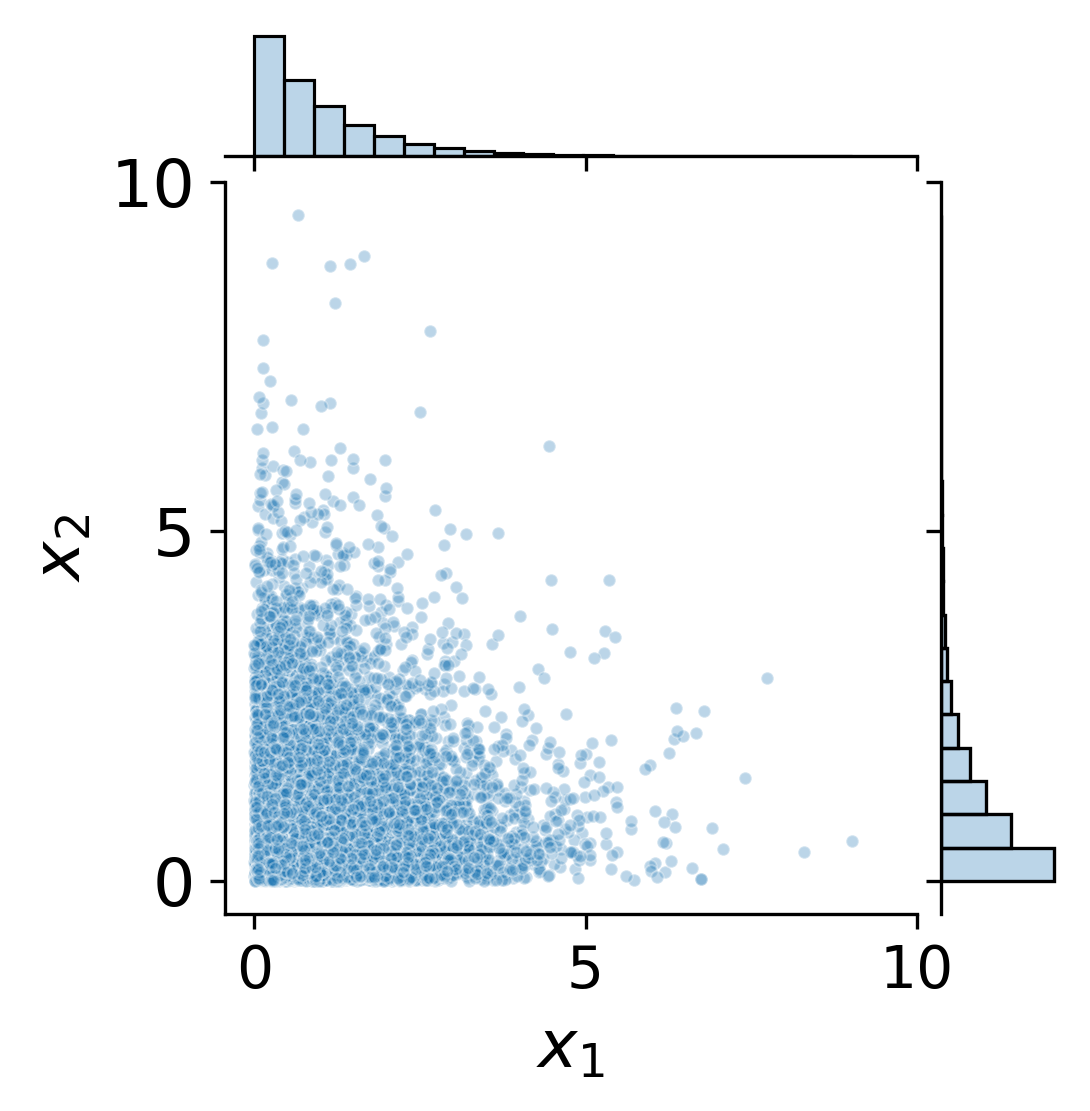
\includegraphics[width=\textwidth]{../numerical_experiments/chapter1/figures/independent_copula.png}
        \caption{Independent copula}
    \end{subfigure}
    \hfill
    \begin{subfigure}[b]{0.32\textwidth}
        \centering
        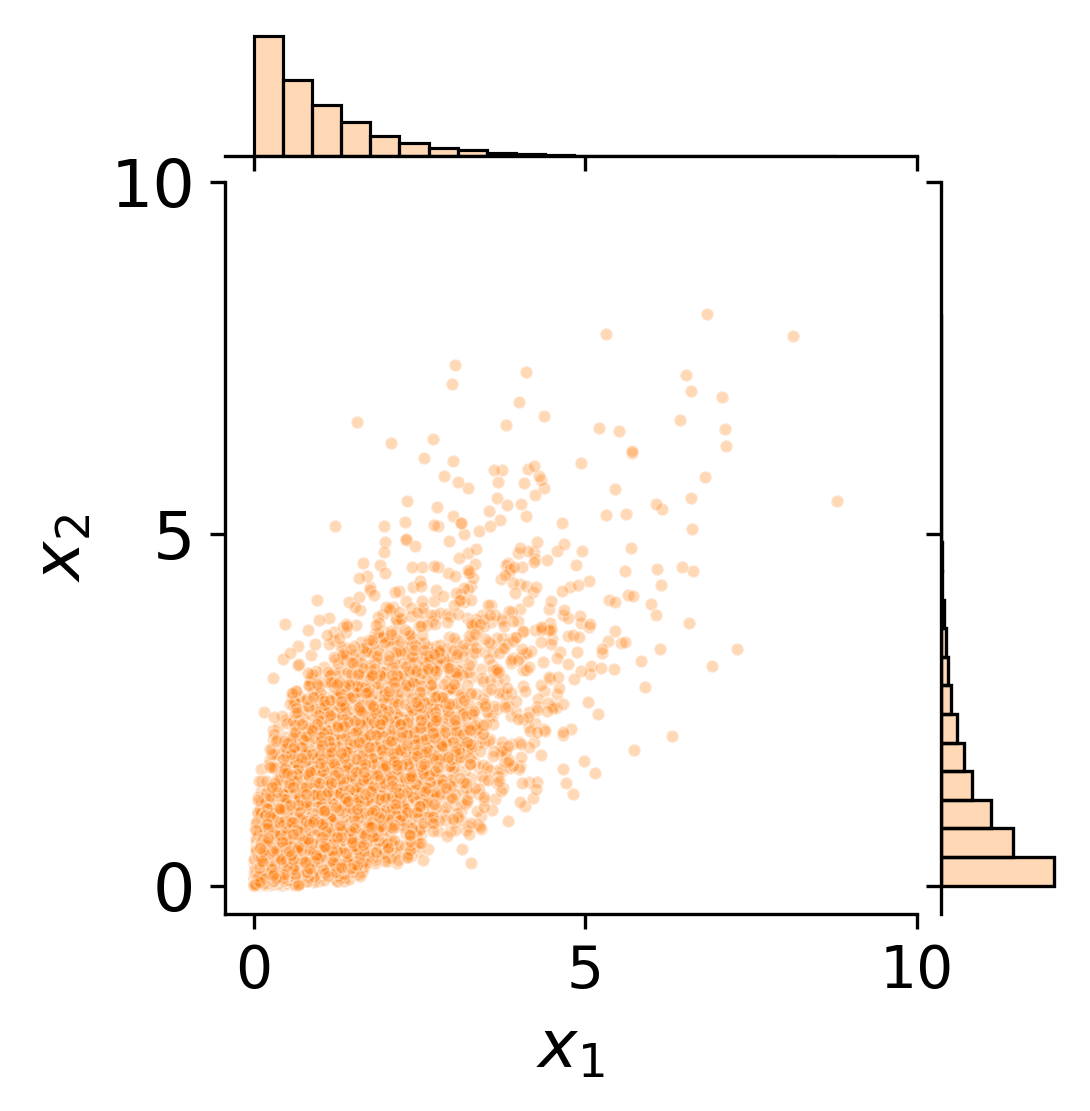
\includegraphics[width=\textwidth]{../numerical_experiments/chapter1/figures/normal_copula.png}
        \caption{Normal copula}
    \end{subfigure}
    \hfill
    \begin{subfigure}[b]{0.32\textwidth}
        \centering
        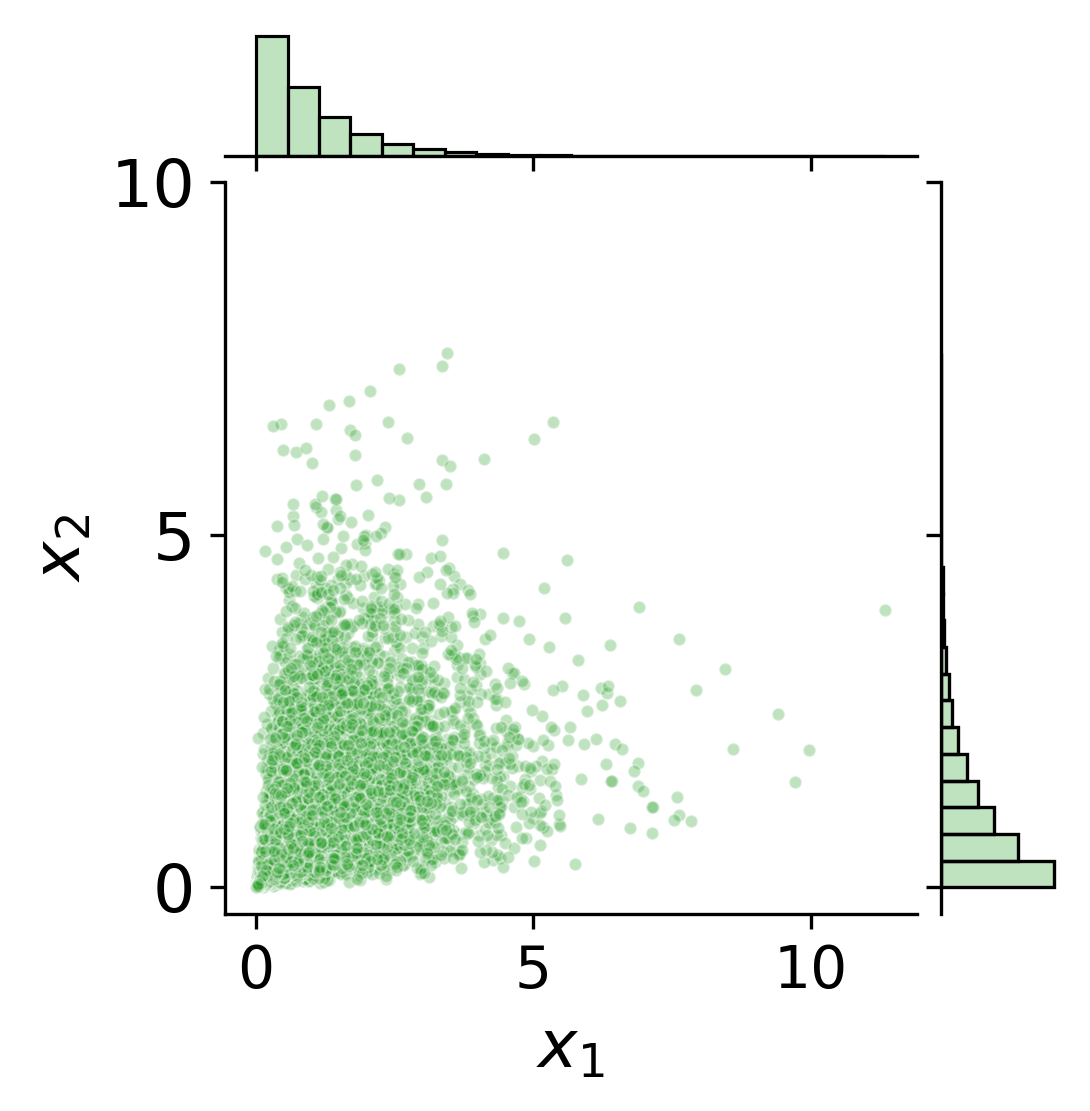
\includegraphics[width=\textwidth]{../numerical_experiments/chapter1/figures/clayton_copula.png}
        \caption{Clayton copula}
    \end{subfigure}
       \caption{Samples of three joint distributions with identical marginals and different dependence structures}
       \label{fig:joint_dist_samples}
\end{figure}

An empirical way of isolating the three dependence structures from this example is to transform the samples in the ranked space. 
Let us consider a $n$-sized sample $\bX_n = \left\{\bx^{(1)}, \dots, \bx^{(n)}\right\} \in \iD_{\bx}^{n}$. 
The corresponding ranked sample is defined as: $\bR_n = \left\{\br^{(1)}, \dots, \br^{(n)}\right\}$, 
where\footnote{The \textit{indicator function} is defined such that $\1_{\left\{\mathcal{A}\right\}}(x) = 1$ if $x \in \mathcal{A}$ and is equal to 0 otherwise.} 
$r^{(l)}_j = \sum_{i=1}^n \1_{\left\{x^{(i)}_j \leq x^{(l)}_j\right\}},$ $\forall j \in \{1, \dots d\}$.
Ranking a multivariate dataset allows us to isolate the dependence structure witnessed empirically. 
\fig{fig:ranked_joint_dist_samples} shows the same three samples from \fig{fig:joint_dist_samples} in the ranked space.
One can first notice that the marginals are uniform since each rank is uniformly distributed. 
Then, the scatter plot from the distribution with independent copula (left plot) is uniform while the two others present different patterns. 
\begin{figure}[ht]
    \centering
    \begin{subfigure}[b]{0.32\textwidth}
        \centering
        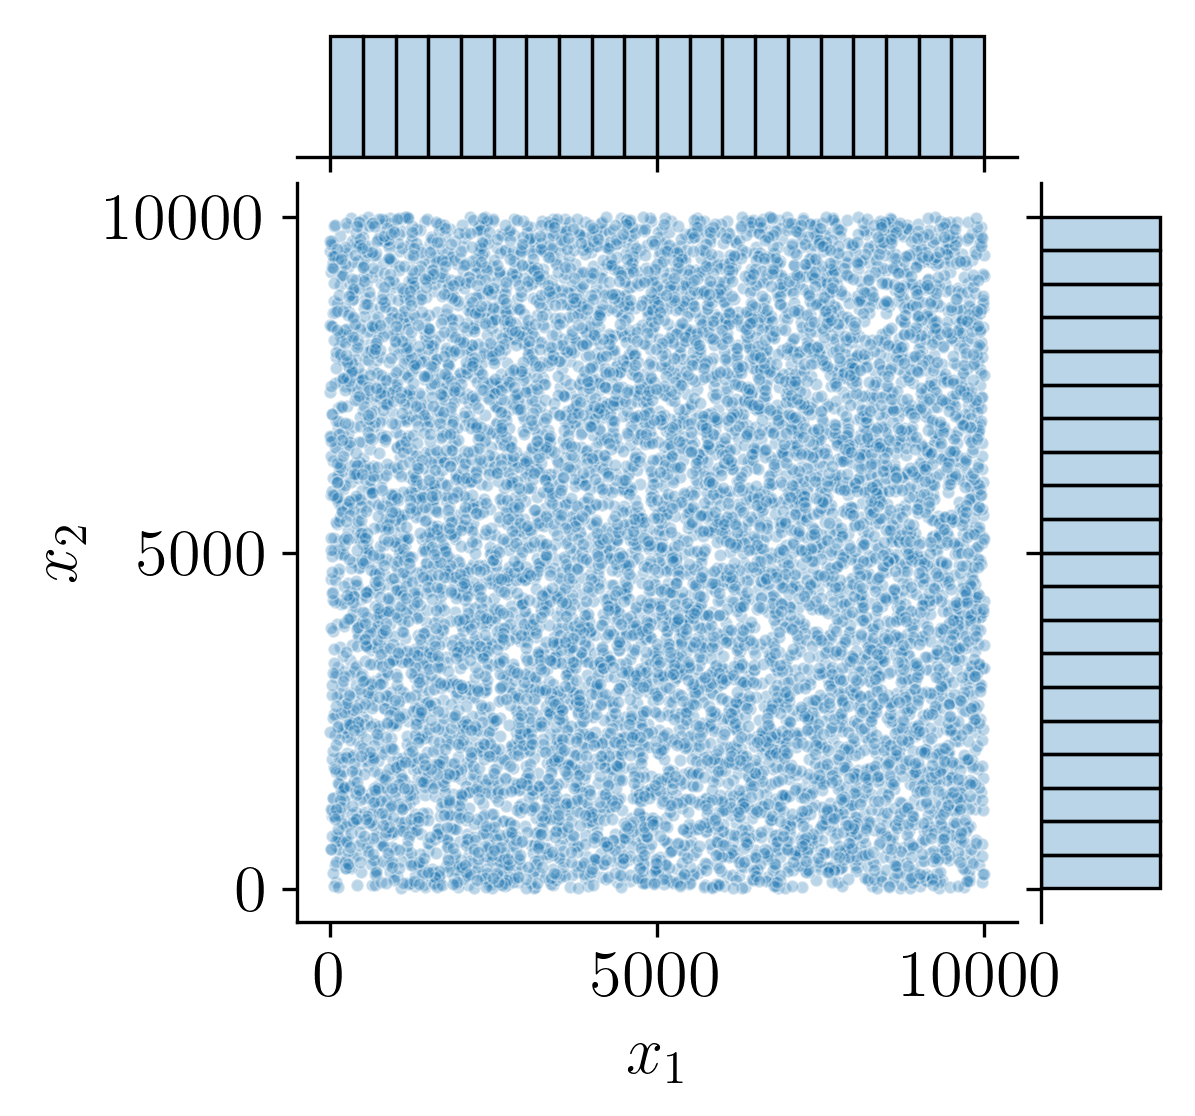
\includegraphics[width=\textwidth]{../numerical_experiments/chapter1/figures/independent_copula_ranked.png}
        \caption{Independent copula}
    \end{subfigure}
    \hfill
    \begin{subfigure}[b]{0.32\textwidth}
        \centering
        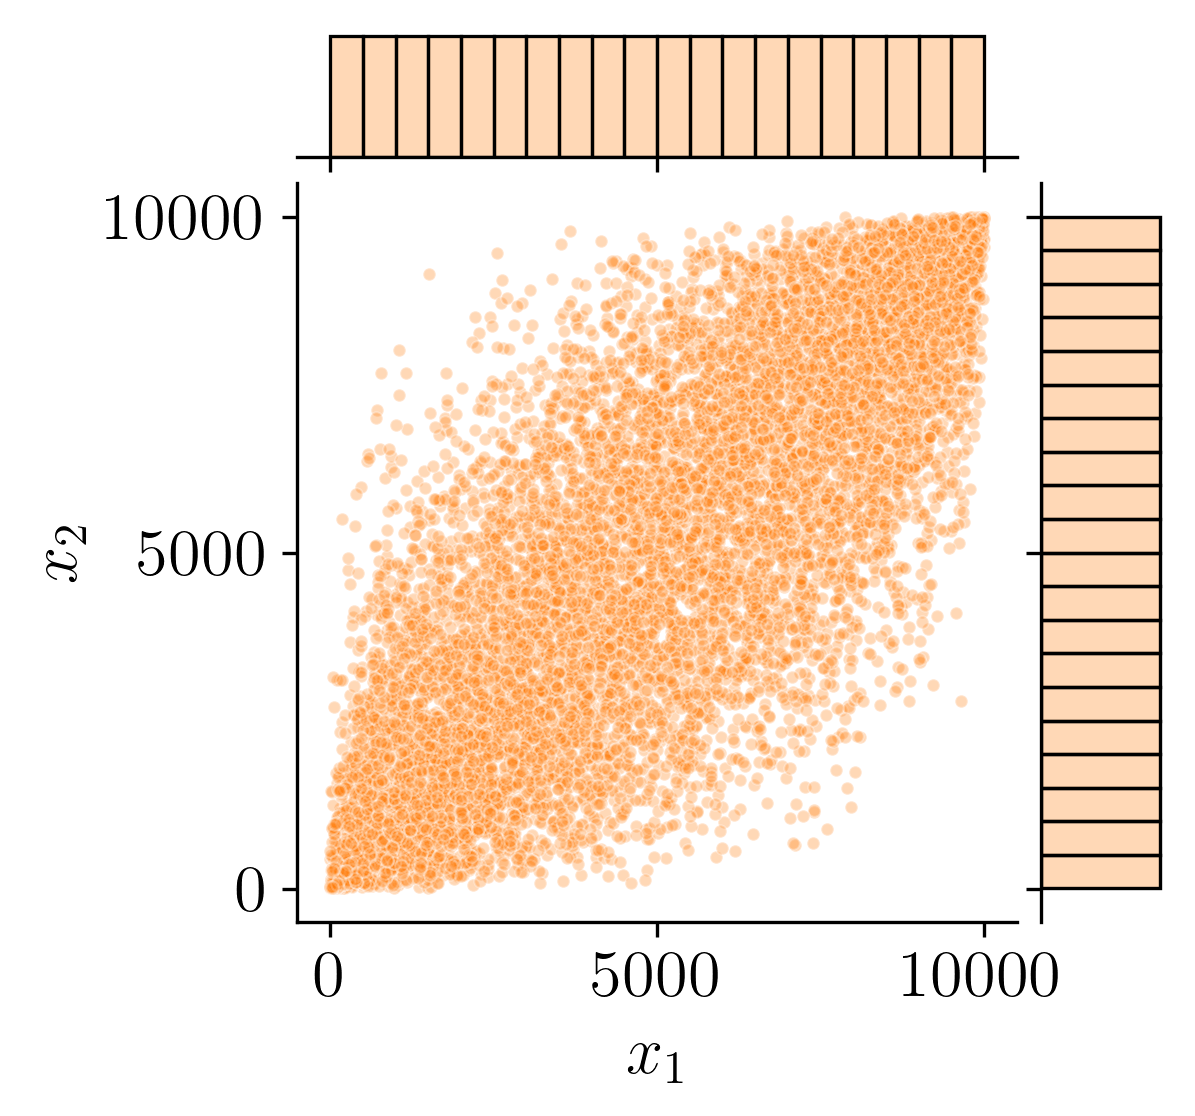
\includegraphics[width=\textwidth]{../numerical_experiments/chapter1/figures/normal_copula_ranked.png}
        \caption{Normal copula}
    \end{subfigure}
    \hfill
    \begin{subfigure}[b]{0.32\textwidth}
        \centering
        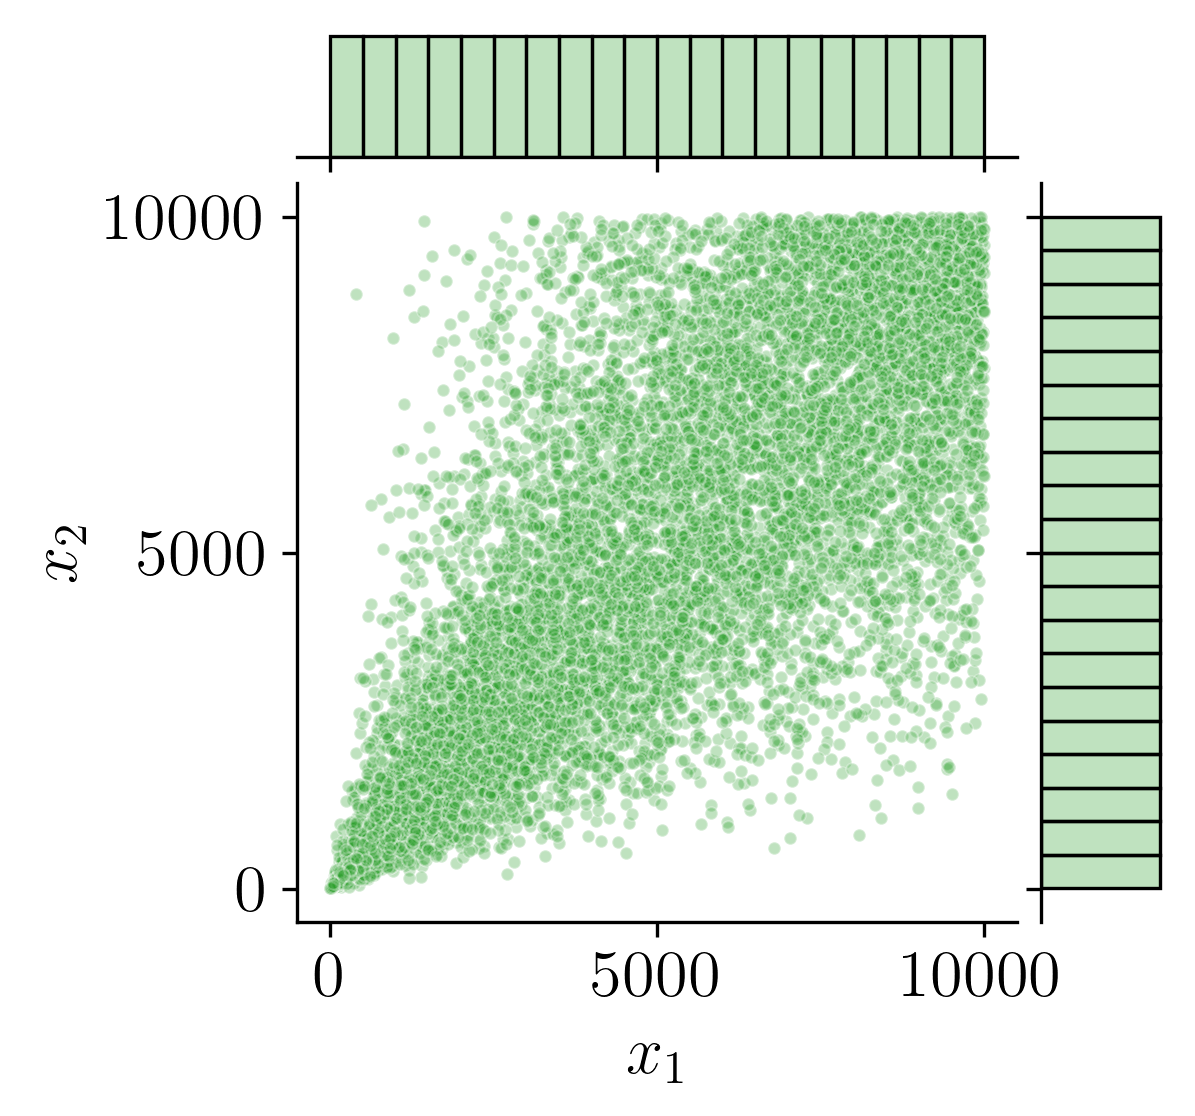
\includegraphics[width=\textwidth]{../numerical_experiments/chapter1/figures/clayton_copula_ranked.png}
        \caption{Clayton copula}
    \end{subfigure}
       \caption{Ranked samples represented in the \fig{fig:joint_dist_samples}}
       \label{fig:ranked_joint_dist_samples}
\end{figure}

A theorem states that the multivariate distribution of any random vector can be broken down into two objects \citep{joe_1997}. 
First, a set of univariate marginal distributions describing the behavior of the individual variables;
Second, a function describing the dependence structure between all variables: a copula. 

\begin{theorem}[Sklar's theorem]
    Let $\mathbf{X} \in \R^d$ be a random vector and its joint CDF $F_{\bX}$ with marginals $\{F_{X_j}\}_{j=1}^d$, there exists a copula $C: [0, 1]^d \rightarrow [0, 1]$, such that:
    \begin{equation}
        F_{\bX}(x_1, \dots, x_d) = C\left(F_{X_1}(x_1), \dots, F_{X_d}(x_d)\right). 
    \end{equation}
    If the marginals $F_{X_i}$ are continuous, then this copula is unique.
    \label{thm:sklar}
\end{theorem}

Theorem \ref{thm:sklar} expresses the joint CDF by combining marginal CDFs and a copula, which is practical for sampling joint distributions. 
Conversely, the copula can be defined by using the joint CDF and the marginal CDFs: 
\begin{equation}
    C(u_1, \dots, u_d) = F_{\bX}(F^{-1}_{X_1}(u_1), \dots, F^{-1}_{X_d}(u_d))
\end{equation}
This equation allows us to extract a copula from a joint distribution by knowing its marginals.
Additionally, copulas are invariant under creasing transformations. 
This property is important to understand the use of rank transformation to display the copula without the marginal effects.     

\elias{define the copula density and address the warning on the confusion.}

Identically to the univariate continuous distributions, a large catalog of families of copulas exists (e.g., independent, Normal, Clayton, Frank, Gumbel copula, etc.).

\elias{define the independent copula, also called a product of marginals.}

To infer a joint distribution, this theorem divides the fitting problem into two independent problems: fitting the marginals and fitting the copula
Provided a dataset, this framework allows the combination of a parametric (or nonparametric) fit of marginals with a parametric (or nonparametric) fit of the copula. 

Appendix \ref{apx:A} details the main techniques to estimate marginal distributions. 
Then, Appendix \ref{apx:B} introduces different nonparametric methods to infer a copula, including the empirical Bernstein copula and the Beta copula. 
The adequation between a fitted probabilistic model and a dataset should be validated, therefore, appendices \ref{apx:A} and \ref{apx:B} respectively present visual and quantitative tools for goodness-if-fit evaluation.

To infer a joint distribution over a dataset, the analyst should determine a fitting strategy.
Smart data visualization helps to choose the fitting methods susceptible to be relevant to the problem. 
The following points can be checked at this early stage: 
\begin{itemize}
    \item Is the distribution unimodal? If not, mixtures methods or nonparametric models might be required;
    \item Is the validity domain restrictive? If so, specific families of parametric distributions can be chosen or truncations can be applied;
    \item Is the dimension high? If the dimension is too high: tensorize the distribution as much as possible.
    \item Is the dependence structure complex? Graphically, the dataset in the ranked space gives an empirical description but some independence tests exist as well. 
\end{itemize} 



%============================================================%
%============================================================%
\section{Central tendency uncertainty propagation}
%============================================================%
%============================================================%

The previous section aimed at building a probabilistic model of the uncertainties considering the knowledge available.
This one will introduce diverse forward propagation of uncertainty through a numerical model. 
This step is hereafter qualified as ``global'' because the analysis of the resulting output random variable will particularly focus on its central tendency (i.e., expected value and variance).
This approach contrasts with the uncertainty propagation dedicated to rare event estimation, which will be introduced in the next section (e.g., for a reliability or certification problem).

The difficulties related to any uncertainty propagation mostly arise from the practical properties of the numerical model. 
Its potential high dimension, low regularity and nonlinearities each represent a challenge. 
These studies rely on a finite number of observations which depends on the computational budget the analyst can afford.   
This forward propagation might be a finality of the uncertainty quantification, but keep in mind that it fully stands on an accurate uncertainty modeling.
Uncertainty propagation should be perceived as a standardized process with modular bricks, on which the ``garbage in, garbage out'' concept fully applies.

This section introduces the main methods of global uncertainty propagation. 
Outlining the strong links between numerical integration (i.e., Lebesgue integration or central tendency estimation) and numerical design of experiments. 


%============================================================%
\subsection{Numerical integration}
%============================================================%

Forward uncertainty propagation aims at integrating a measurable function $g: \iD_{\bX} \rightarrow \R$ with respect to a probability measure $\mu$.
Numerical integration brings algorithmic tools to help the resolution of this probabilistic integration (i.e., Lebesgue integration). 

In practice, this integral is approximated by summing a finite $n$-sized set of realizations $\by_n = \left\{g(\bx^{(1)}), \dots, g(\bx^{(n)})\right\}$ from a set of input samples $\bX_n = \left\{\bx^{(1)}, \dots, \bx^{(n)}\right\}$. 
A \textit{quadrature} establishes a rule to select the input samples $\bX_n$ (also called nodes), and an associated set of weights $\bw_n = \{w_1, \dots, w_n\} \in \R^n$. 
The approximation given by a quadrature rule is defined as a weighted arithmetic mean of the realizations:
\begin{equation}
    I_{\mu}(g) := \int_{\iD_\bX} g(\bx) \dd\mu(\bx) \approx \sum_{i=1}^n w_i g\left(\bx^{(i)}\right).
    \label{eq:quadrature_rule}
\end{equation}
For a given sample size $n$, our goal is to find a set of tuples $\left\{\bx^{(i)}, w_i \right\}_{i=1}^n$ (i.e., quadrature rule), giving the best approximation of our quantity. 
Ideally, the approximation quality should be fulfilled for a wide class of integrands. 
Most quadrature rules only depend on the measure space $(\Omega, \iA, \mu)$, regardless of the integrand values.
In the context of a costly numerical model, this property allows the analyst to massively distribute the calls to the numerical model. 

This section aims at presenting the main multivariate numerical integration techniques. 
These methods have very different properties: 
some are deterministic and some are aleatory; 
some are sequential (or nested) some are not; 
some are victims of the curse of dimensionality and some are not. 
\elias{A summary table of the different methods and their respective properties is proposed ADD REF TO TABLE}.

%\item Some quadratures define negative weights, which can introduce numerical instabilities when $n$ gets large.
%\item The nature of the probability measure (i.e., presence of dependence) might restrict the use of methods

%------------------------------------------------------------%
\subsubsection{Classical multivariate deterministic quadrature}
%------------------------------------------------------------%

Historically, quadrature methods have been developed for univariate integrals. 
The Gaussian rule and the Fejér-Clenshaw-Curtis rule are two univariate deterministic quadratures that will be briefly introduced. 

%Let us first mention the Newton-Cotes quadratures, generalizing multiple rules (e.g., the trapezoidal rule, Simpson's rule, etc.).
Gaussian quadrature is a powerful univariate quadrature building together a set of irregular nodes and a set of weights. 
The computed weights are positive, which ensures a numerically stable rule even for large sample sizes.

Different variants of rules exist, the most famous being the Gauss-Legendre quadrature. 
In this case, the function $g$ to be integrated with respect to the uniform measure on $[-1, 1]$ is approximated by Legendre polynomials.
Considering the Legendre polynomial of order $n$, denoted $l_n$, the quadrature nodes ${x^{(i)}}_{i=1}^n$ are given by the polymonial roots.
The respective weights are given by the following formula: 
\begin{equation}
    w_{i}={\frac {2}{\left(1-\left(x^{(i)}\right)^{2}\right)\left(l'_{n}(x^{(i)})\right)^{2}}}.
\end{equation}
This rule guarantees a very precise approximation provided that the integrand is well-approximated by a polynomial of degree $2n-1$ or less on $[-1, 1]$.
This rule is deterministic but not sequential, meaning that two rules with sizes $n_1$ and $n_2$, $n_1 < n_2$ will not be nested. 
However, a sequential extension is proposed by the Gauss-Kronrod rule \citep{laurie_1997}, offering lower accuracy. 

To overcome this practical drawback, Fejér then Clenshaw with Curtis proposed a nested rule with mostly equivalent accuracy as Gaussian quadrature.
This method is usually presented to integrate a function with respect to the uniform measure on $[-1, 1]$ and starts with a change of variables:
\begin{equation}
    \int_{-1}^{1} g(x) \, \dd x = \int_{0}^{\pi} g(\cos(\theta)) \sin(\theta) \, \dd \theta 
\end{equation}
This expression can be written as an expansion of the integrand using cosine series. 
Moreover, cosine series are closely related to the Chebyshev polynomials of the first kind. 
Fejér's ``first rule'' \citep{trefethen_2008} relies on the Chebyshev polynomials roots as nodes $x^{(i)} = \cos(\theta^{(i+1/2)})$, and the following weights:
\begin{equation}
    w_i=\frac{2}{n}\left(1-2\sum_{j=1}^{\lfloor n/2 \rfloor}\frac{1}{4j^2-1}\cos\left(j\theta^{(2i+1)}\right)\right)    
\end{equation}
These two univariate integration schemes are both very efficient on a wide panel of functions. 
Yet, Fejér-Clenshaw-Curtis is sequential and offers easy implementations, benefitting from powerful algorithms such as the \textit{fast Fourier transform}. 

\begin{figure}[ht]
    \centering
    \begin{subfigure}[b]{0.32\textwidth}
        \centering
        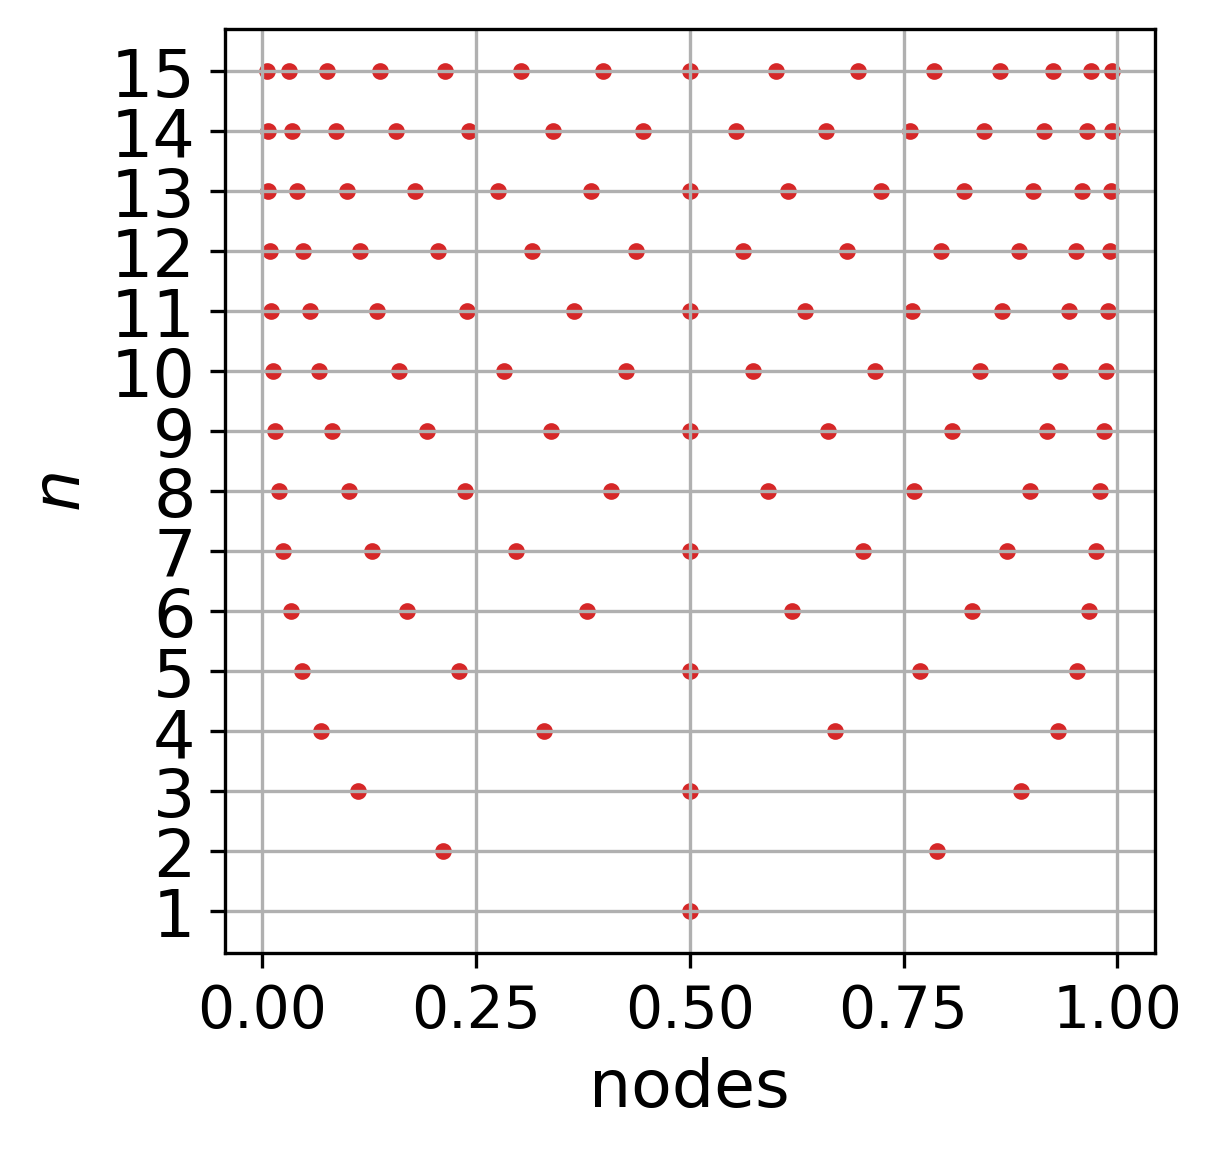
\includegraphics[width=\textwidth]{../numerical_experiments/chapter1/figures/univariate_gauss_legendre.png}
        \caption{Gauss-Legendre}
    \end{subfigure}
    \quad
    \begin{subfigure}[b]{0.32\textwidth}
        \centering
        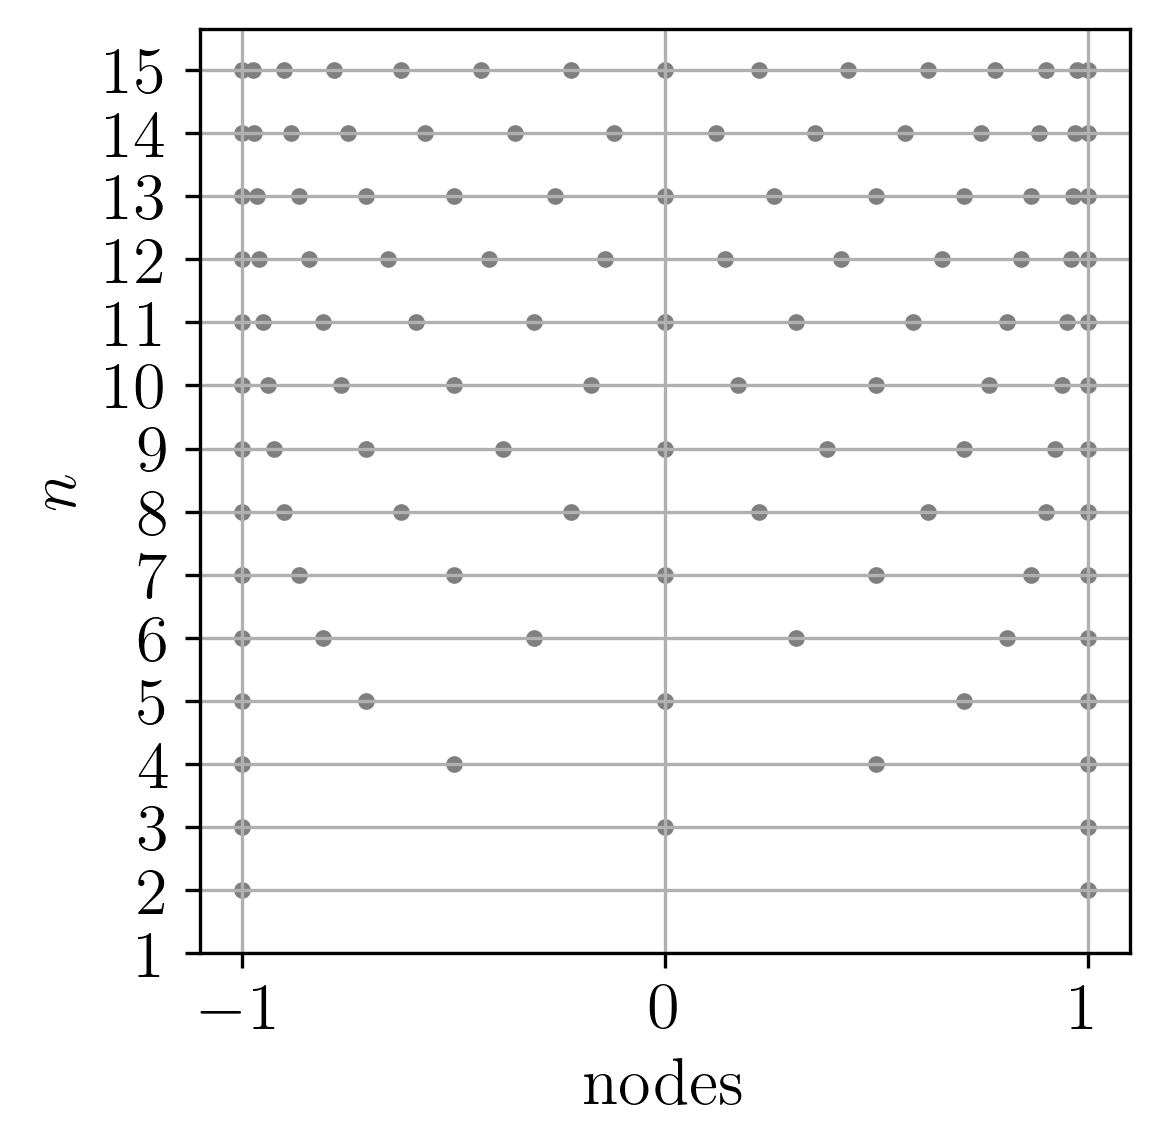
\includegraphics[width=\textwidth]{../numerical_experiments/chapter1/figures/univariate_clenshaw_curtis.png}
        \caption{Clenshaw-Curtis}
    \end{subfigure}
    \caption{Univariate quadratures nodes ($1 \leq n \leq 15$)}
    \label{fig:univariate_quads}
\end{figure}


Uncertainty quantification problems are rarely unidimensional, but one can build a multivariate quadrature rule by defining the tensor product (also called full grids) of univariate rules. 
This exhaustive approach quickly shows its practical limits as the problem's dimension increases. 
Alternatively, sparse multivariate quadratures (i.e., Smolyak sparse grid) explore the joint domain more efficiently. 



%------------------------------------------------------------%
\subsubsection{Monte Carlo methods}
%------------------------------------------------------------%
Monte Carlo methods were initially developed in the 1940s to solve problems in neutronics.  
Ever since this frequentist techniques have been applied to the resolution of the Lebesgue integral. 
To integrate a function $g$ against a measure $\mu$, it randomly generates points following the input measure. 
The integral is estimated by taking the uniform arithmetic mean of the images of these nodes obtained by this random process. 

This aleatory method requires to be able to generate points following a given distribution. 
To do so, the most common approach is to first generate a sequence of random points uniformly on $[0, 1]$. 
These sequences mimic actual uniform randomness but are in fact generated by deterministic algorithms (also called pseudorandom number generators).
Pseudorandom algorithms generate a sequence of numbers with a very large, but finite length. 
This sequence can be exactly repeated by fixing the same initial point, also called \textit{pseudorandom seed}.
Most programming languages use the Mersenne Twister pseudorandom generator \citep{matsumoto_1998}, offering a very long period (around $4.3\times10^{6001}$ iterations).

Formally, the ``Vanilla'' Monte Carlo (sometimes called ``crude'' Monte Carlo) method uses a set of i.i.d samples $\bX_n = \left\{\bx^{(1)}, \dots, \bx^{(n)}\right\}$ following the joint distribution of $\mu$. 
The Monte Carlo estimator of the integral is given by: 
\begin{equation}
    I_{\mu}(g) \approx \Bar{y}_n^{\textrm{MC}} = \frac1n \sum_{i=1}^{n} g(\bx^{(i)}).
\end{equation}
By construction, the law of large numbers makes this estimator unbiased, however, it converges relatively slowly. 
Considering the images of the sample $\bX_n$, one can also estimate the variance of the output random variable $\what{\sigma}^2_Y$.
The variance of the Monte Carlo estimator results from a manipulation of the central tendency theorem:
\begin{equation}
    \var\left(\Bar{y}_n^{\textrm{MC}}\right) = \frac{1}{\sqrt{n}} \var\left(g(\bX)\right). 
\end{equation}
This estimator also comes with theoretical confidence intervals at $\alpha \%$, regardless of the output distribution: 
\begin{equation}
    I_{\mu}(g) \in \left[\Bar{y}_n^{\textrm{MC}}  - q_\alpha \frac{\var\left(g(\bX)\right)}{\sqrt{n}}, \Bar{y}_n^{\textrm{MC}}  + q_\alpha \frac{\var\left(g(\bX)\right)}{\sqrt{n}} \right],
\end{equation}
where $q_\alpha$ is the $\alpha$-quantile of the standard normal distribution.
Monte Carlo presents the advantage of being a universal method, with no bias and strong convergence guarantees. 
Moreover, it is worth noting that its convergence properties do not depend on the dimension of the input domain. 
Unlike the previous multivariate deterministic quadrature, Monte Carlo doesn't suffer from the curse of dimensionality. 
The main limit of crude Monte Carlo is its convergence speed, making it untractable in most practical cases. 
More recent methods aim at keeping the interesting properties of this technique while making it more efficient.
Among the \textit{variance reduction} family of methods, let us mention importance sampling, stratified sampling (e.g., latin hypercube sampling), control variates and multi-level Monte Carlo (see Chapters 8, 9 and 10 from \citet{owen_2013} and \citep{giles_2008}).


%------------------------------------------------------------%
\subsubsection{Quasi-Monte Carlo and Koksma-Hlawka inequality}
%------------------------------------------------------------%

Among the methods presented so far, classical deterministic quadratures are subject to the curse of dim while Monte Carlo methods deliver contrasted performances. 
Quasi-Monte Carlo is a deterministic family of numerical integration schemes over $[0, 1]^d$ with respect to the uniform measure on $[0, 1]$. 
It offers powerful performances with strong guarantees by choosing nodes respecting \textit{low discrepancy} sequences. 

The discrepancy of a set of nodes (or a design) can be seen as a metric of its uniformity. 
The lowest the discrepancy of a design is, the ``closest'' it is to uniformity. 

The Koksma-Hlawka theorem \citep*{morokoff_1995,leobacher_2014} is a fundamental result for understanding the role of the discrepancy in numerical integration. 
\begin{theorem}[Koksma-Hlawka]
    If $g:[0, 1]^d\rightarrow\R$ has a bounded variation (i.e., its total variation is finite), then for any design $\bX_n = \left\{\bx^{(1)}, \dots, \bx^{(n)}\right\} \in [0, 1]^d$:
    \begin{equation}
        \left| \int_{[0, 1]^d} g(\bx) \ddx - \frac1n \sum_{i=1}^n g\left(\bx^{(i)}\right)\right| \leq  V(g) D^*(\bX_n).
        \label{eq:KH_inequality}
    \end{equation}

    Where $D^*(\bX_n)$ is the star discrepancy of the design $\bX_n$, while $V(g)$ quantifies the complexity of the integrand, which is related to its total variation. 
\end{theorem}

Where the function variation $V(g)$ in the \eq{eq:KH_inequality} can formally be defined as the Hardy-Klause variation: 
\begin{equation}
    V(g) = \sum_{\mathfrak{u}\subseteq\{1, \dots, p \}} \int_{[0, 1]^\mathfrak{u}} \left| \frac{\partial^{\mathfrak{u}}g}{\partial \bx_{\mathfrak{u}}}(\bx_{\mathfrak{u}}, 1)\right| \dd\bx.
\end{equation}

Where the \textit{$L_p$ star discrepancy} of a design $\bX_n$ defined as the $L_p$-norm of the difference between the empirical CDF of the design $\what{F}_{\bX_n}$ and the CDF of the uniform distribution $F_{\textbf{U}}$:  
\begin{equation}
    D^*_p(\bX_n) = \lVert \what{F}_{\bX_n} - F_{\textbf{U}}\rVert _p = \left(\int_{[0, 1]^d} \lvert\what{F}_{\bX_n}(\bx) - F_{\textbf{U}}(\bx)\rvert ^p \, \ddx \right)^{1/p}.
\end{equation}
Additionally, the $L_\infty$ star discrepancy can be defined from a geometric point of view. 
Let us consider the number of a design $\bX_n$, falling in a subdomain $[\mathbf{0}, \bx)$ as $\#(\bX_n \cap [\mathbf{0}, \bx))$. 
Then, this empirical quantification is compared with the volume of the rectangle $[\mathbf{0}, \bx)$, noted $\mathrm{vol}\left([\mathbf{0}, \bx)\right)$.  
Finally, this star discrepancy is written:   
\begin{equation}
    D^*(\bX_n) = \sup_{\bx \in [0, 1]^d} \left| \frac{\#(\bX_n \cap [\mathbf{0}, \bx))}{n} - \mathrm{vol}\left([\mathbf{0}, \bx)\right)\right|
\end{equation}
\elias{Figure xx empirically represents discrepancy concept}
Let us point out that this star discrepancy is equivalent to the Kolmogorov-Smirnov test verifying whether the design follows a uniform distribution. 

\noindent
One can notice how the Koksma-Hlawka inequality dissociates the quadrature performance into a contribution from the function complexity and one from the repartition of the quadrature nodes. 
Knowing that the complexity of the studied integrand is fixed, this property explains the motivation to generate low-discrepancy quadratures in numerical integration.  

Note that the design can also be considered as a discrete distribution (uniform sum of Dirac distributions).
The discrepancy can then be expressed as a probabilistic distance between this discrete distribution and the uniform distribution. 
A generalized discrepancy between distributions will be presented in the \elias{Part 2}.

Some famous low-discrepancy sequences (e.g., van der Corput, Halton, Sobol', Faure, etc.) can offer a bounded star discrepancy $D^*(\bX_n) \leq \frac{C \log(n)^d}{n}$, with $C$ a constant depending on the sequence.
Therefore, using these sequences as a quadrature rule with uniform weights provides the following absolute error upper bound: 
\begin{equation}
    \left| \int_{[0, 1]^d} g(\bx) \ddx - \frac1n \sum_{i=1}^n g\left(\bx^{(i)}\right)\right| \leq  \frac{V(g) \log(n)^d}{n}
\end{equation}

%This bound is qualified as sharp since for any design $\bX_n$, and every $\epsilon > 0$, a function $g$ with variation $V(g)=1$ exists such that:
%\begin{equation}
%    \left| \int_{[0, 1]^d} g(\bx) \ddx - \frac1n \sum_{i=1}^n g\left(\bx^{(i)}\right)\right|  > D^*(\bX_n) - \epsilon.
%\end{equation} 

The generation of these sequences doesn't necessarily require more effort than pseudo-random sampling.
Chapter 15 in \citet{owen_2013} offers an extended presentation of the ways to generate different low-discrepancy sequences. 
For example, the van der Corput and Halton sequences rely on congruential generators. 
%Then, scrambling procedures are sometimes implemented to correct pathologies famously observed on Halton sequences. 
To overcome the limits of Halton sequences, digital nets such as the famous Sobol' or Faure sequences have been developed.  
Sobol' sequences are in base two and have the advantage of being extensible in dimension. 
Note that by construction, these sequences offer significantly lower discrepancies for specific values. 
Typically designs with sizes equal to powers of two or power of prime numbers will be favorable. 
To illustrate the different patterns and properties of different methods, \fig{fig:quasi_monte_carlo_designs} represents the three designs of 256 points. 
Each is split into the first 128 points (in red) and the following 128 points (in black) to show to nested properties of the QMC sequences.

\begin{figure}[ht]
    \centering
    \begin{subfigure}[b]{0.32\textwidth}
        \centering
        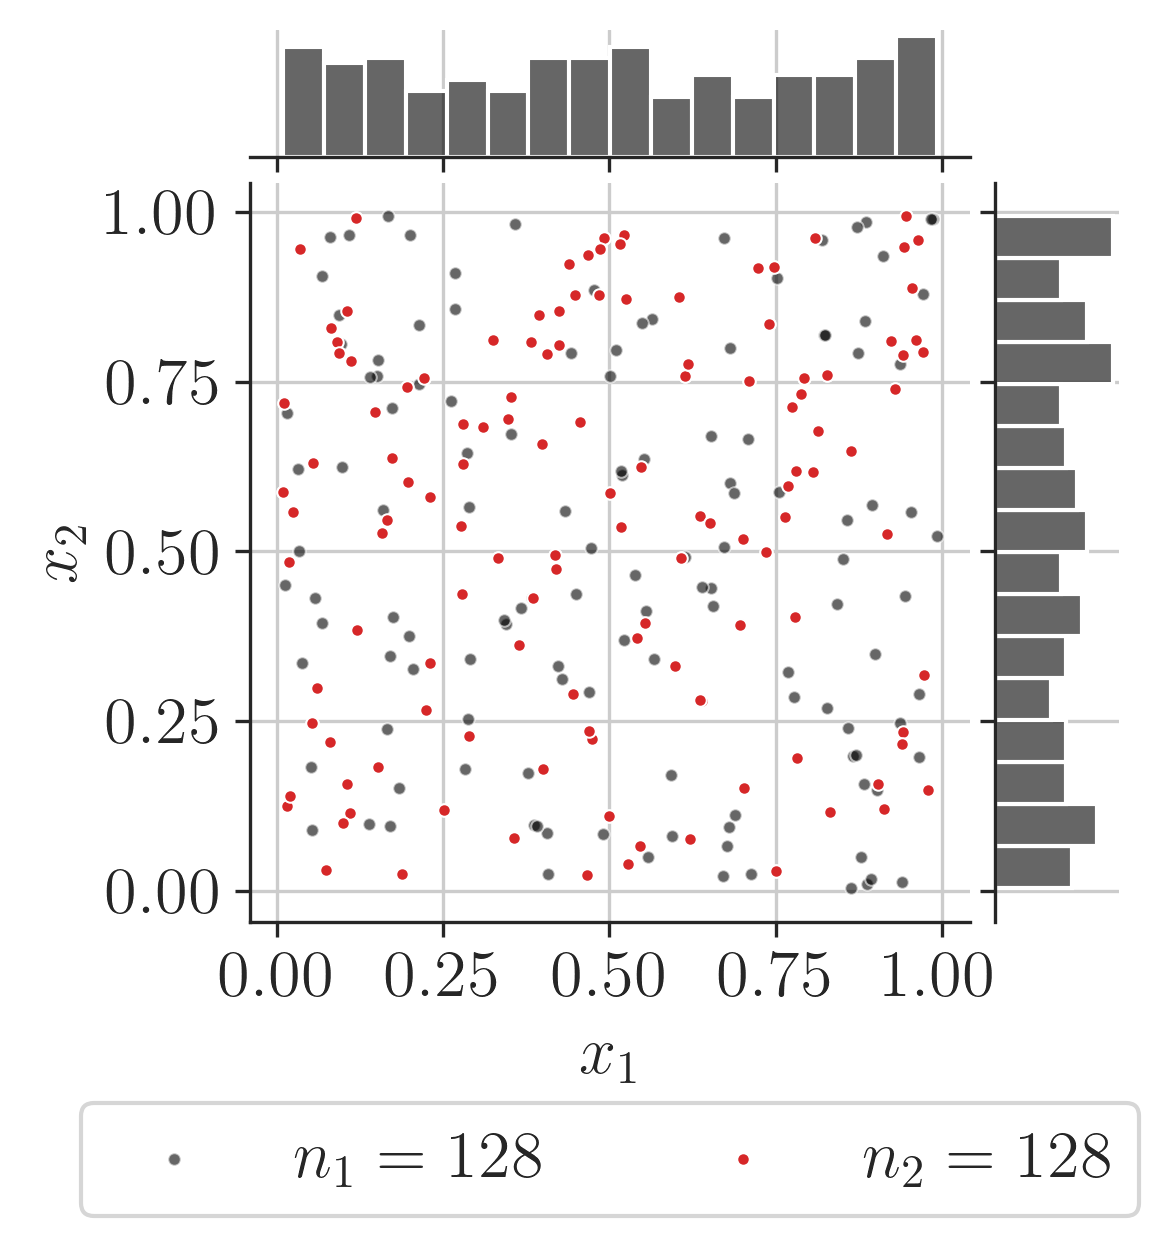
\includegraphics[width=\textwidth]{../numerical_experiments/chapter1/figures/MonteCarlo256.png}
        \caption{Monte Carlo}
    \end{subfigure}
    \hfill
    \begin{subfigure}[b]{0.32\textwidth}
        \centering
        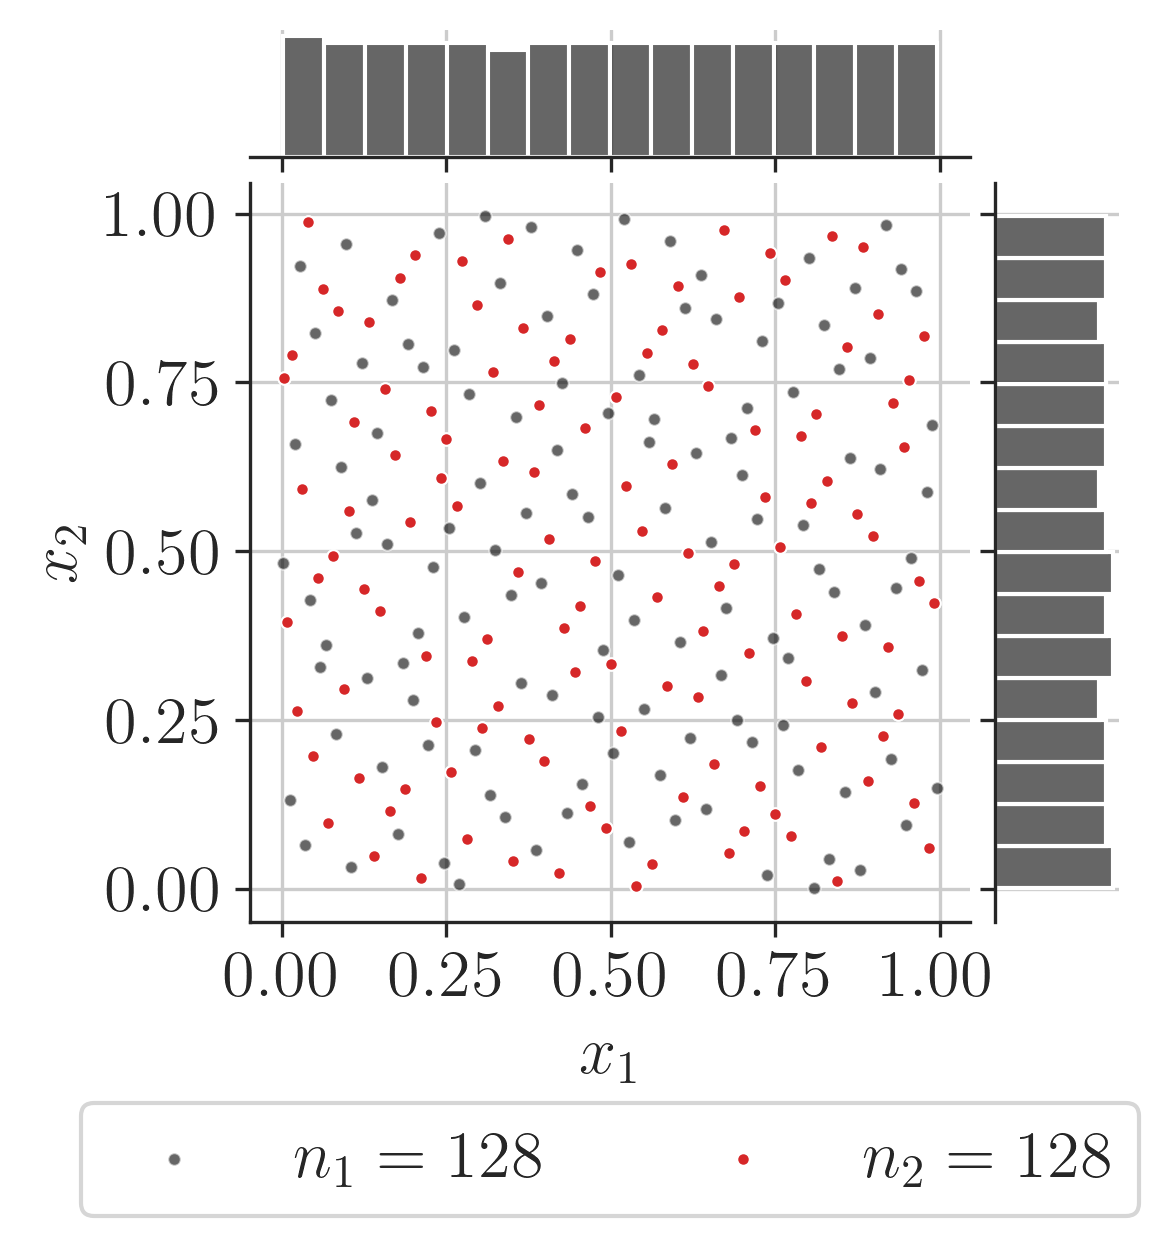
\includegraphics[width=\textwidth]{../numerical_experiments/chapter1/figures/quasi_MonteCarlo_Halton_256.png}
        \caption{Halton sequence}
    \end{subfigure}
    \hfill
    \begin{subfigure}[b]{0.32\textwidth}
        \centering
        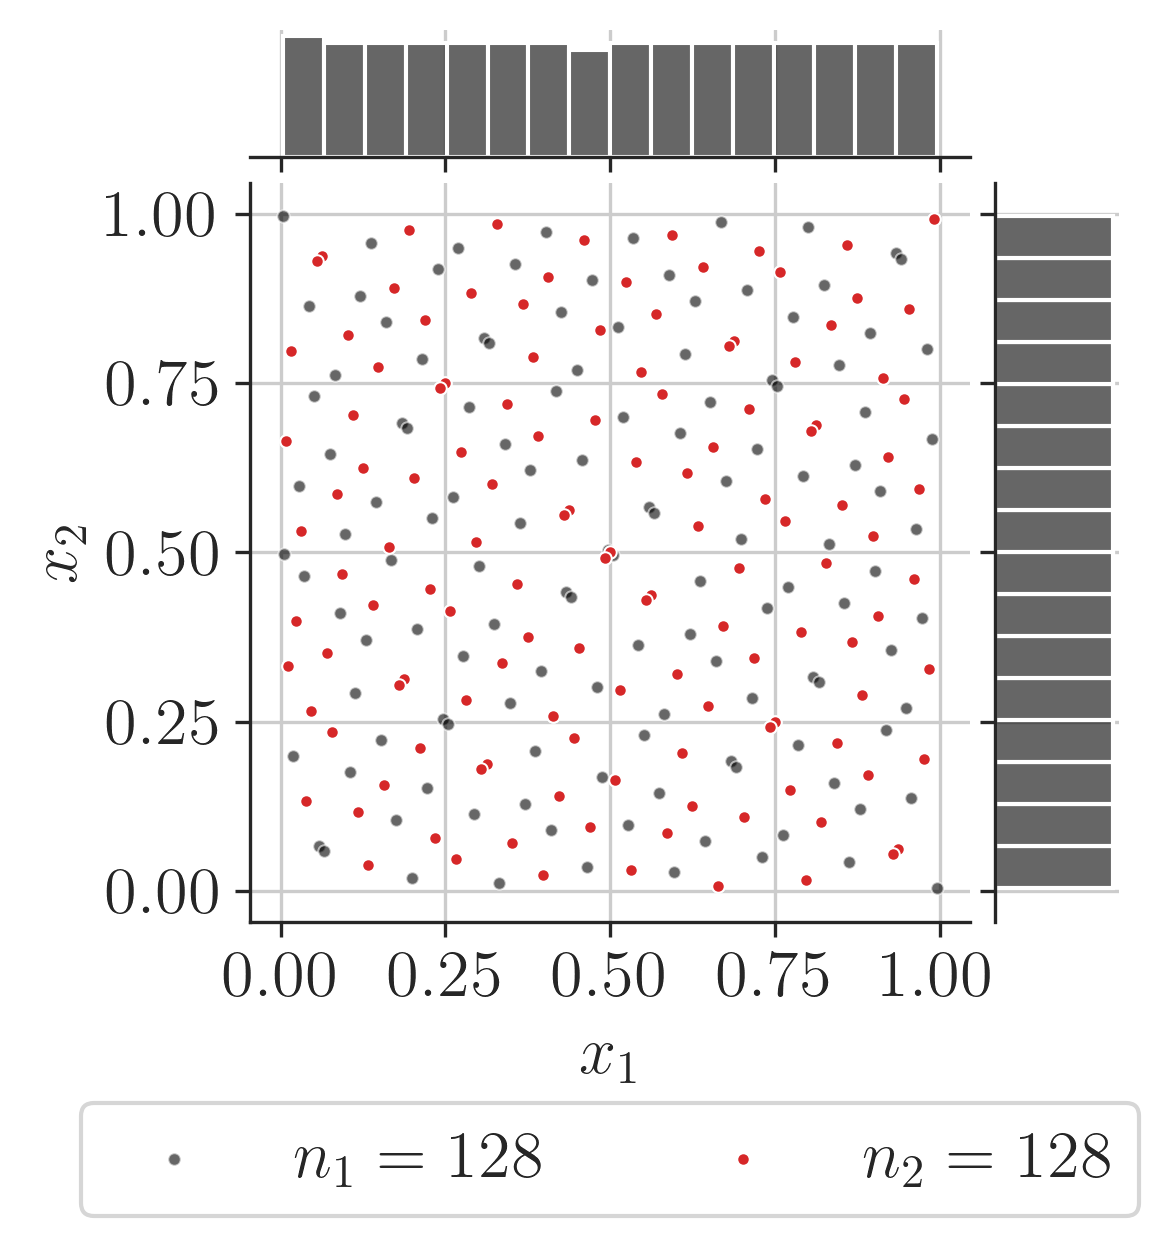
\includegraphics[width=\textwidth]{../numerical_experiments/chapter1/figures/quasi_MonteCarlo_256.png}
        \caption{Sobol' sequence}
    \end{subfigure}
       \caption{Nested Monte Carlo and quasi-Monte Carlo designs ($n=256$)}
       \label{fig:quasi_monte_carlo_designs}
\end{figure}

A quantity estimated by crude MC comes with some associated confidence. 
This complementary information is essential to deliver an end-to-end uncertainty quantification and misses in QMC methods.  
\textit{Randomized quasi-Monte Carlo} (RQMC) is a method adding some randomness in QMC in order to compute confidence intervals while benefiting from a low variance.
A specific review of the randomized (also called ``scrambled'') QMC is proposed by \citet{lecuyer_2018}. Various authors recommend the use of RQMC by default instead of QMC as a good practice. 
Recent works aim at exploring the use of these methods to estimate different quantities of interest (such as an expected value \citep{gobet_2022} or a quantile \citep{tuffin_2019})

Quasi-Monte Carlo methods easily generate powerful integration schemes. 
The KH inequality associates an upper bound and a convergence rate to most integrals. 
A randomization overlay fades the deterministic property of these designs to allow confidence interval computation.
In the following, sampling techniques are presented from the numerical \textit{design of experiments} point of view. 
Even if the finality might look different from the previous numerical integration, it shares many methods and concepts. 



%============================================================%
\subsection{Numerical design of experiments}
%============================================================%
The numerical design of experiments aims at exploring uniformly the input domain, e.g., to build the learning set of a regression model, or to initialize a multi-start optimization strategy. 
A design of experience (also simply called design) is then qualified as \textit{space-filling} when it properly covers a domain. 
As well as in integration, a design of experiments allows propagating uncertainties through a numerical model (or an actual experiment from a laboratory test bench). 
However, a difference comes from the fact that this community often works with designs of very limited sizes. 
Users of designs of experiments might also need to build designs with various properties. 
\begin{itemize}
    \item Some might be interested in the sequentiality of a sampling method, to eventually add new points as they get a computational budget extension.
    \item Some might request a sampling method conserving its properties in any sub-domains. 
    This second property can be useful to reduce the problem's dimension by dropping a few unimportant marginals.
\end{itemize}

Different metrics are commonly used to quantify how space-filling a design of experiments is. 
The previously introduced different types of discrepancies are space-filling metrics.
Other types of space-filling metrics rely on purely geometrical considerations.  

This section will first define some space-filling metrics.
Secondly, the \textit{latin hypercube sampling} (LHS) will be introduced as a variance-reduction that became popular in this community. 
Finally, a general discussion on uncertainty propagation with respect to non-uniform measures will be presented.

%------------------------------------------------------------%
\subsubsection{Space-filling metrics and properties}
%------------------------------------------------------------%
Space-filling criteria are key to evaluating designs and are often used in their construction to optimize their performances. 
In the previous section, the star discrepancy was introduced as a distance of a finite design to uniformity.
However, the $L_\infty$ star discrepancy is hard to estimate, fortunately, \citet{warnock_1972} elaborated an explicit expression specific to the $L_2$ star discrepancy: 
\begin{equation}
    \left[D^*_2(\bX_n)\right]^2 = \frac19 - \frac2n \sum_{i=1}^{n} \prod_{l=1}^{d} \frac{(1-x_l^{(i)})}{2} + \frac{1}{n^2}\sum_{i,j=1}^{n} \prod_{l=1}^{d} \left[1 - \max(x_l^{(i)}, x_l^{(j)})\right].
\end{equation}
One can notice that this expression is similar to the Cramér-von Mises test statistic. 
Even if this expression is tractable, \citet{fang_liu_2018} detailed its limits. 
First, the star $L_2$ discrepancy generates designs that are not robust to projections in sub-spaces. 
Then, this metric is not invariant in rotation and reflection. 
Finally, by construction, $L_p$ discrepancies give a special role to the point $\mathbf{0}$ by anchoring the box $[\mathbf{0}, \bx)$.

Two improved criteria were proposed by \citet{hickernell_1998} with the \textit{centered $L_2$ discrepancy} and the \textit{wrap-around $L_2$ discrepancy}.
Those are widely used in practice since they solve the previous limits while satisfying the Koksma-Hlawka inequality with a modification of the total variation.
Let us introduce the formula of the centered $L_2$ discrepancy:
\begin{multline} CD^*_2(\bX_n)  = \left(\frac{13}{12}\right)^{d} - \frac{2}{n} \sum_{i=1}^{n} \prod_{l=1}^{d} \left( 1 + \frac{1}{2} |x_l^{(i)} - 0.5| - \frac{1}{2} |x_l^{(i)} - 0.5|^2 \right)\\
    + \frac{1}{n^2} \sum_{i,j=1}^{n} \prod_{l=1}^{d} \left( 1 + \frac{1}{2} |x_l^{(i)} - 0.5| + \frac{1}{2} |x_l^{(j)} - 0.5| - \frac{1}{2} |x_l^{(i)} - x_l^{(j)}| \right).
\end{multline}

As an alternative to discrepancies, many geometrical criteria exist to assess a space-filling design.
The most common way to do so is to maximize the minimal distance among the pairs of Euclidian distances between the points of a design.  
The criterion to maximize is then simply called the \textit{minimal distance} of a design (denoted $\phi_{min}$). 
For numerical reasons, the $\phi_p$ criterion is often used instead of the minimal distance. 
The following $\phi_p$ criterion converges towards the minimum distance as $p\geq1$ tends to infinity:
\begin{equation} 
    \phi_{\min}(\bX_n) = \min_{i \neq j} ||\bx^{(i)} - \bx^{(j)}||_2\, , \qquad
    \phi_p(\bX_n) = \sum_{i=1}^{j} \sum_{j=1}^{n} \left( |x^{(i)} - x^{(j)}|^{-p} \right)^{\frac{1}{p}}.
\end{equation}
More space-filling criteria are reviewed in \citet{abtini_2018}. 
These space-filling metrics are widely used to optimize a different sampling technique.


%------------------------------------------------------------%
\subsubsection{Latin hypercube sampling}
%------------------------------------------------------------%
The LHS is a method introduced in 1979 \citep{mckay_beckman_1979}, initially for numerical integration.
This stratified sampling technique forces the distribution of each sub-projection of a bounded domain to be as uniform as possible
To do so, for a $n$-sized design, each marginal's domain is divided into $n$ identical segments.
This creates a regular grid of $n^{d}$ squared cells over the domain. 

An LHS design does not allow more than one point within a segment. 
That way, a new LHS can be built as a permutation of the marginals of an existing LHS.
Inside each selected cell from the grid, the point can be placed in the center or randomly.

Various contributions provided first a variance, then a central limit theorem to the LHS \citep{owen_1996}.
Identically to the Monte Carlo variance\elias{add pointer}, LHS variance can be expressed as:
\begin{equation}
    \var\left(\Bar{y}_n^{\textrm{LHS}}\right) = \frac{1}{\sqrt{n}} \var\left(g(\bX)\right) - \frac{C}{n} + o\left( \frac1n \right). 
\end{equation}
Where $C$ is a positive constant, showing that the LHS usually reduces the variance for numerical integration. 
Because of its stratified structure, LHS can generate poor designs from a space-filling point of view (see e.g., Figure \elias{add diagonal design}). 
The following section presents various methods aiming at optimizing these designs.


%------------------------------------------------------------%
\subsubsection{Optimized Latin hypercube sampling}
%------------------------------------------------------------%
To improve the space-filling property of LHD, it is common to add an optimization step. 
The goal of this optimization is to improve a space-filling criterion by generating LHD from permutations of an initial LHD.
\citet{damblin_couplet_2013} reviews LHS optimization using different discrepancy criteria and subprojection properties.
This optimization can be performed by different algorithms, such as the stochastic evolutionary algorithm or simulated annealing.
The results from this work show that LHD optimized by $L_2$ centered or wrap-around discrepancies offer strong robustness to two-dimensional projections.
It also shows that these designs keep this property for dimensions larger than 10, while scrambled Sobol' sequences lose it. 

More recent work developed different ways to get optimized LHD. 
Let us mention the maximum projection designs from \citet{joseph_gul_2015} and the uniform projection designs from \citet{sun_2019}.
\elias{Add a sentence to explain the concept}

\begin{figure}[ht]
    \centering
    \begin{subfigure}[b]{0.32\textwidth}
        \centering
        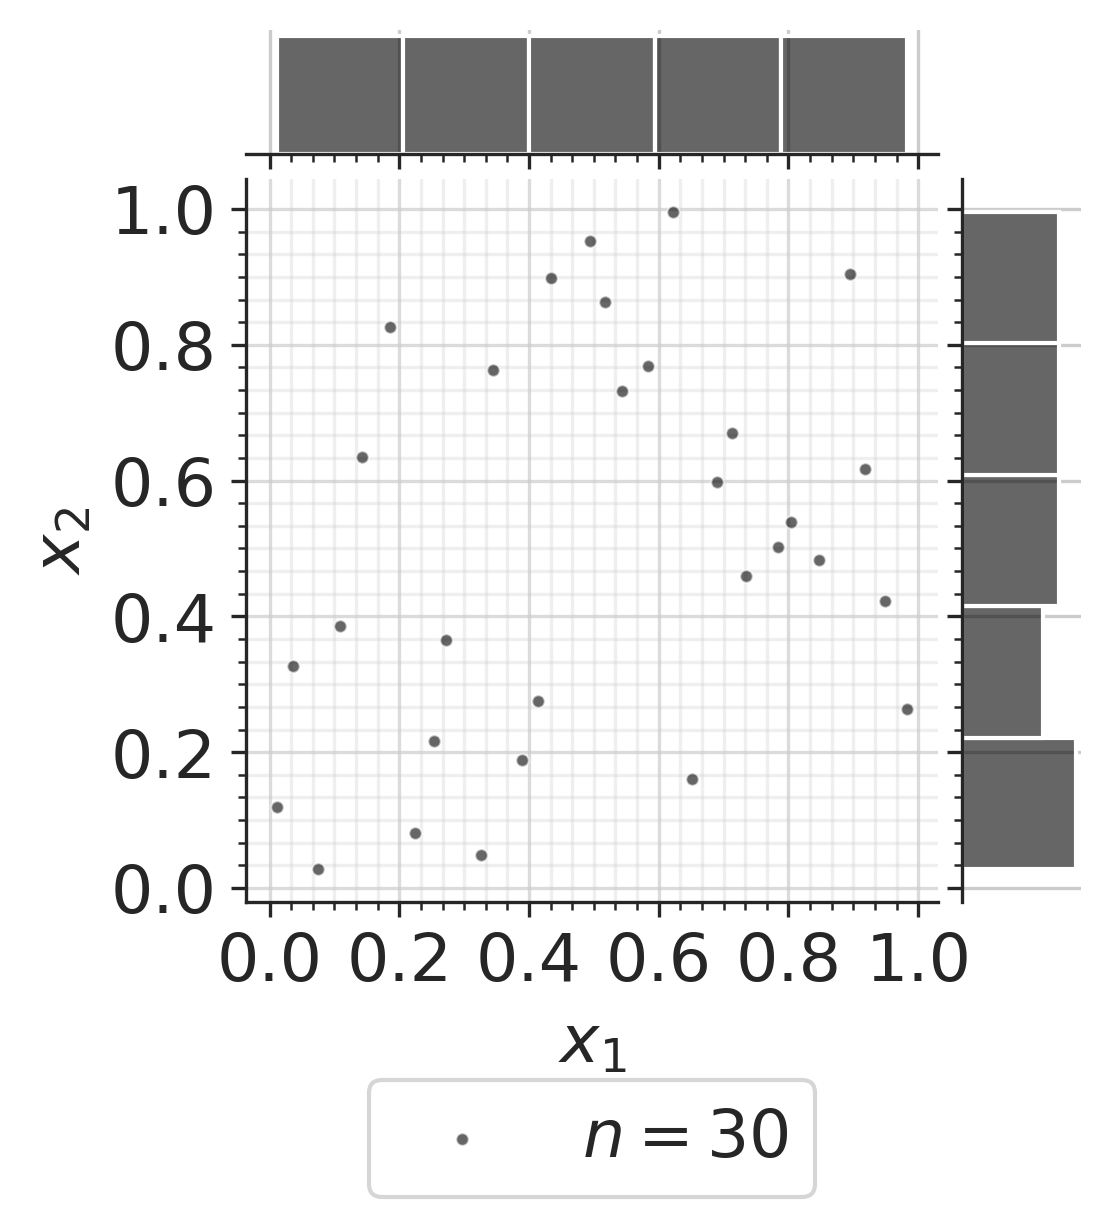
\includegraphics[width=\textwidth]{../numerical_experiments/chapter1/figures/poor_LHS.png}
        \caption{Poorly space-filling LHS}
    \end{subfigure}
    \hfill
    \begin{subfigure}[b]{0.32\textwidth}
        \centering
        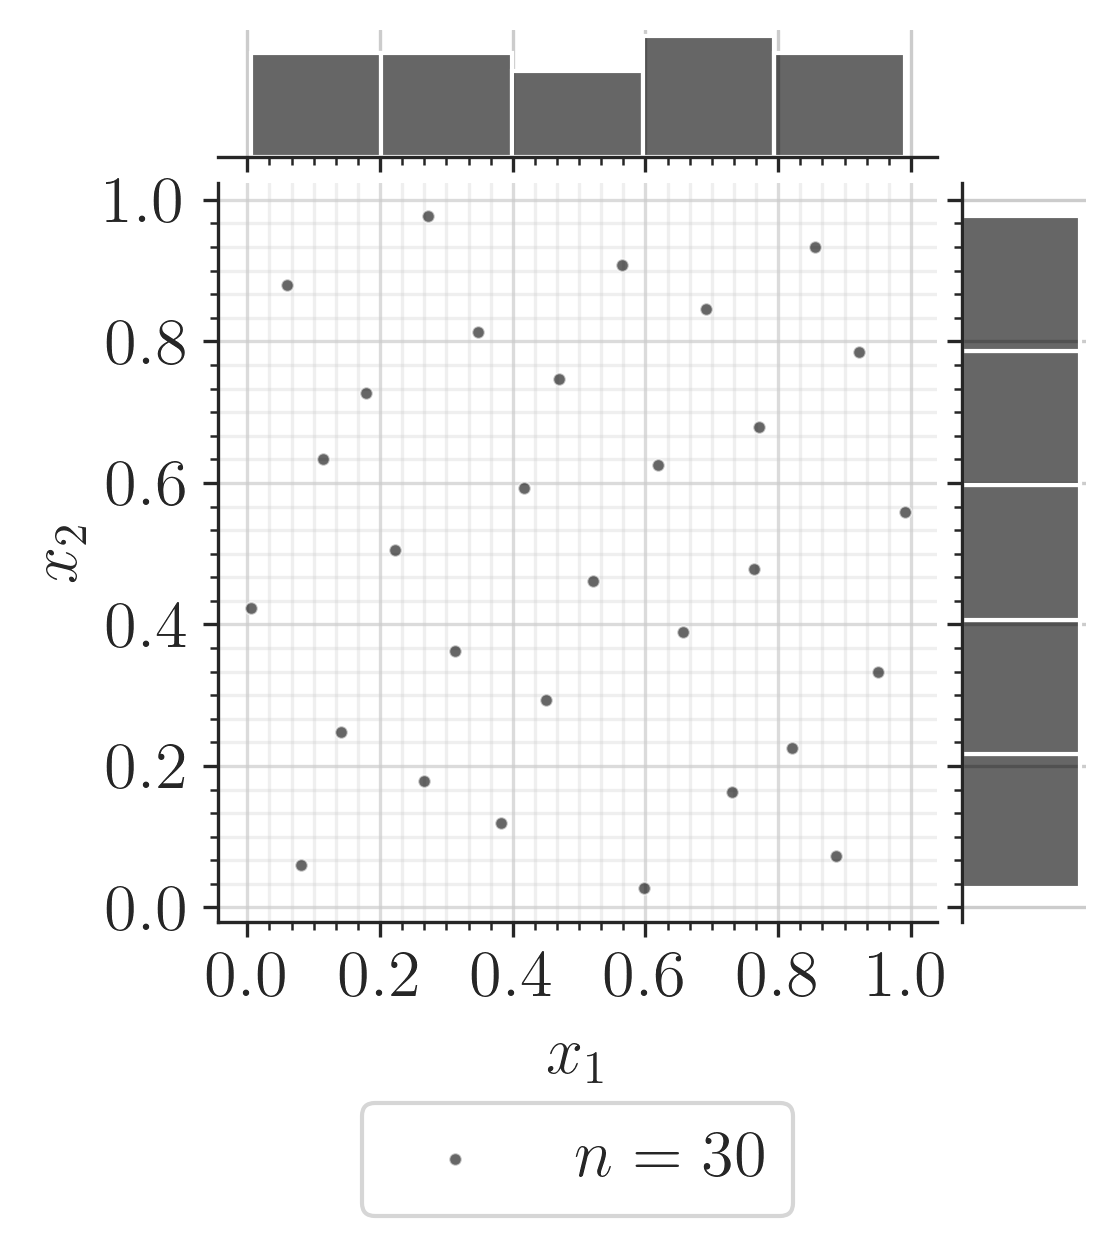
\includegraphics[width=\textwidth]{../numerical_experiments/chapter1/figures/optimized_C2_LHS.png}
        \caption{$L_2$ centered optimized LHS}
    \end{subfigure}
    \hfill
    \begin{subfigure}[b]{0.32\textwidth}
        \centering
        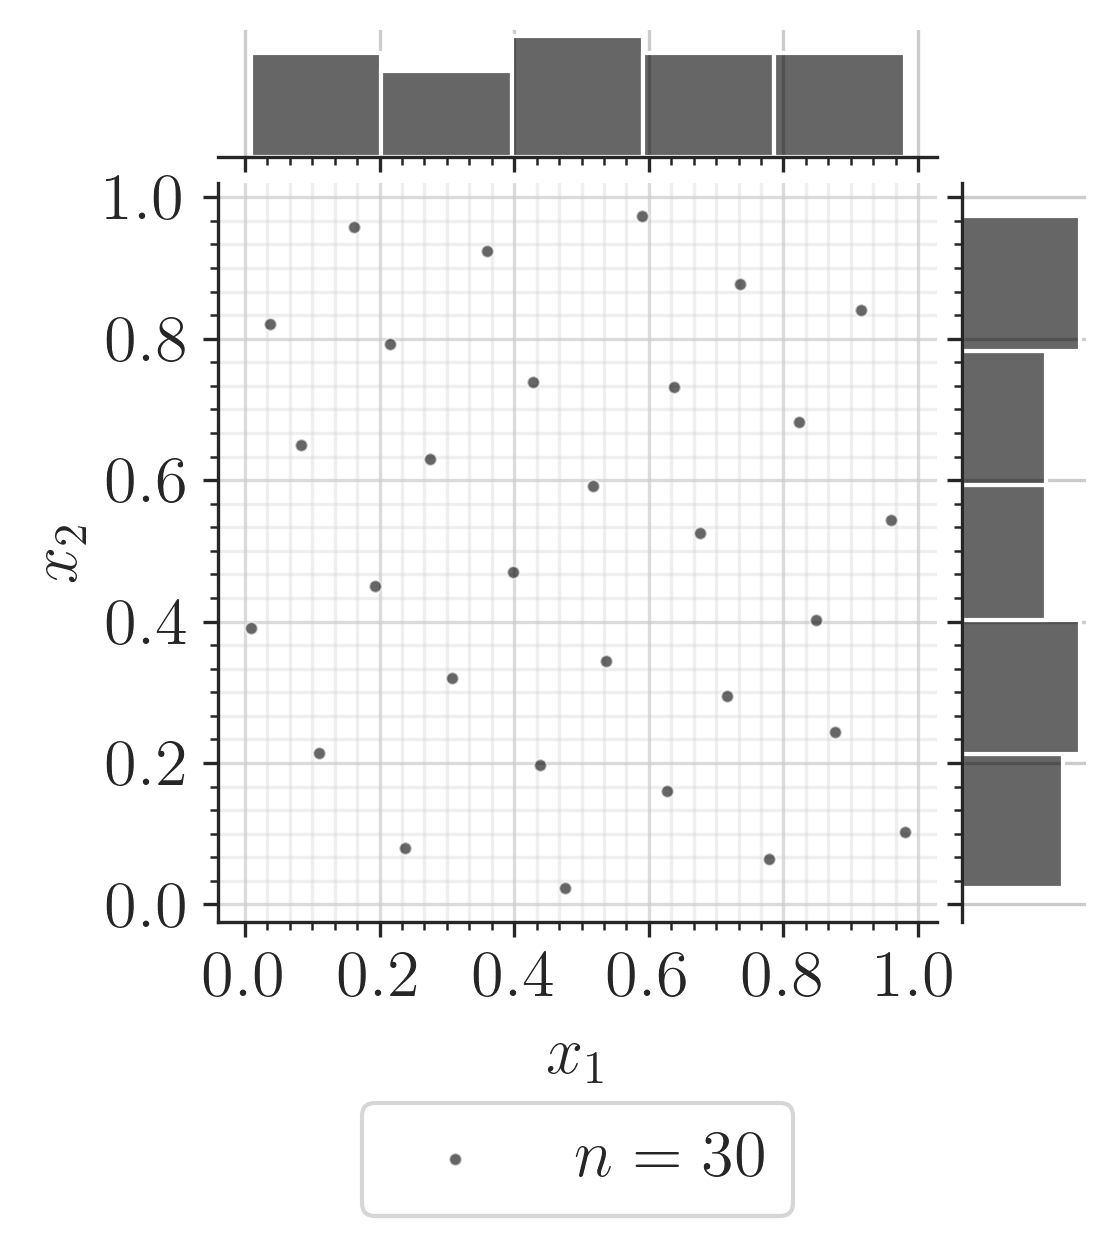
\includegraphics[width=\textwidth]{../numerical_experiments/chapter1/figures/optimized_phip_LHS.png}
        \caption{$\phi_p$ optimized LHS}
    \end{subfigure}
       \caption{Latin hypercube designs with poor and optimized space-filling properties ($n=8$)}
       \label{fig:LHS_designs}
\end{figure}

%============================================================%
\subsection{Summary and discussion}
%============================================================%


A wide panel of sampling techniques exists for numerical integration or design of experiments purposes. 
In both cases, the studied domain was bounded and the targeted measure was uniform. 
However, uncertainty propagation is often performed on complex input distributions, with possibly unbounded domains. 
In uncertainty quantification, this step might be referred to as the estimation of the output random variable's central tendency (i.e., its mean and variance).
Central tendency estimation is a numerical integration with respect to any input distribution, also named \textit{probabilistic integration} by \citet{briol_oates_2019}.  

To generate i.i.d samples following any distribution (i.e., non-uniform), one may use \textit{inverse transform} sampling.
This method first generates a sample in the unit hypercube, then, the inverse CDF function (i.e., quantile function) is applied on marginals. 
Finally, possible dependence effects can be added using the Sklar theorem \eq{thm:sklar}.

One may wonder if the properties from the uniform design are conserved after this nonlinear transformation. 
\citet{hickernell_2020} explores this question from a discrepancy point of view. 
The authors find correspondences between discrepancies with respect to uniformity and discrepancy with respect to the target distribution. 
However this result show practical limits, sometimes making the interpretation of the last discrepancy easier. 
This question will be further discussed using a more general framework in the \elias{Chapter xx}.

Let us also remark that, depending on the distribution, defining the inverse CDF is not always possible.
For example, samples following truncated distributions or mixture distributions might sometime be generated with a different technique. 
The \textit{acceptance-rejection} method offers a versatile generation only based on the PDF $f_{\bx}$.
Assuming that a well-known proposal PDF $f^*_{\bx}$ exists such that $f_{\bx} \leq c \times f^*_{\bx}, c \in [1, +\infty]$. 
Then, one may generate a sample according to $c \times f^*_{\bx}$ and only retain from this sample the points under the PDF $f_{\bx}$.
\elias{add illustration with truncated normal and triangular.}
Note that QMC sampling is not well suited with acceptance-rejection since its structure gets perturbed. 

\begin{itemize}
    \item \elias{Markov Chain Monte Carlo: when it is hard to sample from the distribution.}
    \item \elias{Add the summary table with the properties of each methods?}
\end{itemize}

In this section, many methods were presented to propagate input uncertainties against a deterministic function.
The propagation with the three following goals and contexts were introduced: 
\begin{itemize}
    \item building a quadrature rule for numerical integration against a uniform distribution,
    \item creating a space-filling design of experiments to uniformly explore the space, often in a small data context (e.g., to build the learning set of a surrogate model),
    \item generating a design for central-tendency estimation, which is simply a numerical integration against a non uniform density.
\end{itemize} 
%Note that some of these methods can also find a use in the context of data compression or quantization.
These three objectives have been explored in different communities but actually mostly share similar methods. 
They all have in common the general analysis (i.e., global behavior) of the output random variable. 
However, some studies require to shift the focus on specific areas of the output random variables.
When using uncertainty propagation to perform a risk analysis, the events studied are often contained in the tails of the output distribution. 
In this case, dedicated uncertainty propagation methods will significantly improve the estimation of the associated statistical quantities.


%============================================================%
%============================================================%
\section{Reliability-oriented uncertainty propagation}
%============================================================%
%============================================================%

This section aims at presenting another type of uncertainty propagation. 
In the context of a risk analysis applied to the engineering field, the reliability of a system needs to be assessed. 
Most often, a risk measure associated with a failure mode of the studied system is estimated. 

Since most systems studied in risk analysis should be highly reliable, the occurrence of such event is qualified as rare. 
Only an unlikely small amount of extreme input conditions or an unlikely unfavorable combinations of inputs lead to the failure of the system. 
Hence the usage of the equivalent terms \textit{reliability analysis} and \textit{rare event estimation}. 
The notion of risk associated with an event is often decomposed as a product of likelihood and impact. 
The failure of a system might be very rare but its consequences can be severe (e.g., civil engineering structures, nuclear infrastructure, telecommunication networks, electrical grid, railway signalling, etc.).

Different risk measures (i.e., quantities of interest) can be studied depending on the type of risk analysis. 
Quantiles are a first conservative measure, widely used for risk analysis. 
The $\alpha$-quantile $q_\alpha$ of the output random variable $Y$ is defined as:
\begin{equation}
    q_\alpha = \inf_{y\in\R}{\left\{F_Y(y) \geq \alpha\right\}}, \quad \alpha \in [0, 1].    
\end{equation}
\elias{define superquantiles in text?}
As an alternative, one can define a scalar safety threshold $\yth$ that should not be exceeded to keep the system safe. 
Then, a second risk measure is probability of exceeding this safety threshold, also called \textit{failure probability}: 
\begin{equation}
    \pf = \P\left(Y \geq \yth\right), \quad \yth\in\R.
\end{equation}
To illustrate this quantity, \fig{fig:1D_reliability} shows the one-dimensional propagation of a normal distribution (represented by the PDF on the left), throught a function $g(\cdot)$.
The probability of exceeding a given threshold $\yth$ is represented by the area in red under the output PDF on top.
An interesting reflection on the use and the interpretation of risk measures
\footnote{Including measures from the finance domain such as the \textit{conditional value-at-risk} (also called superquantile).} 
is presented in \citet{rockafellar_2015}. 

\begin{figure}
    \centering
    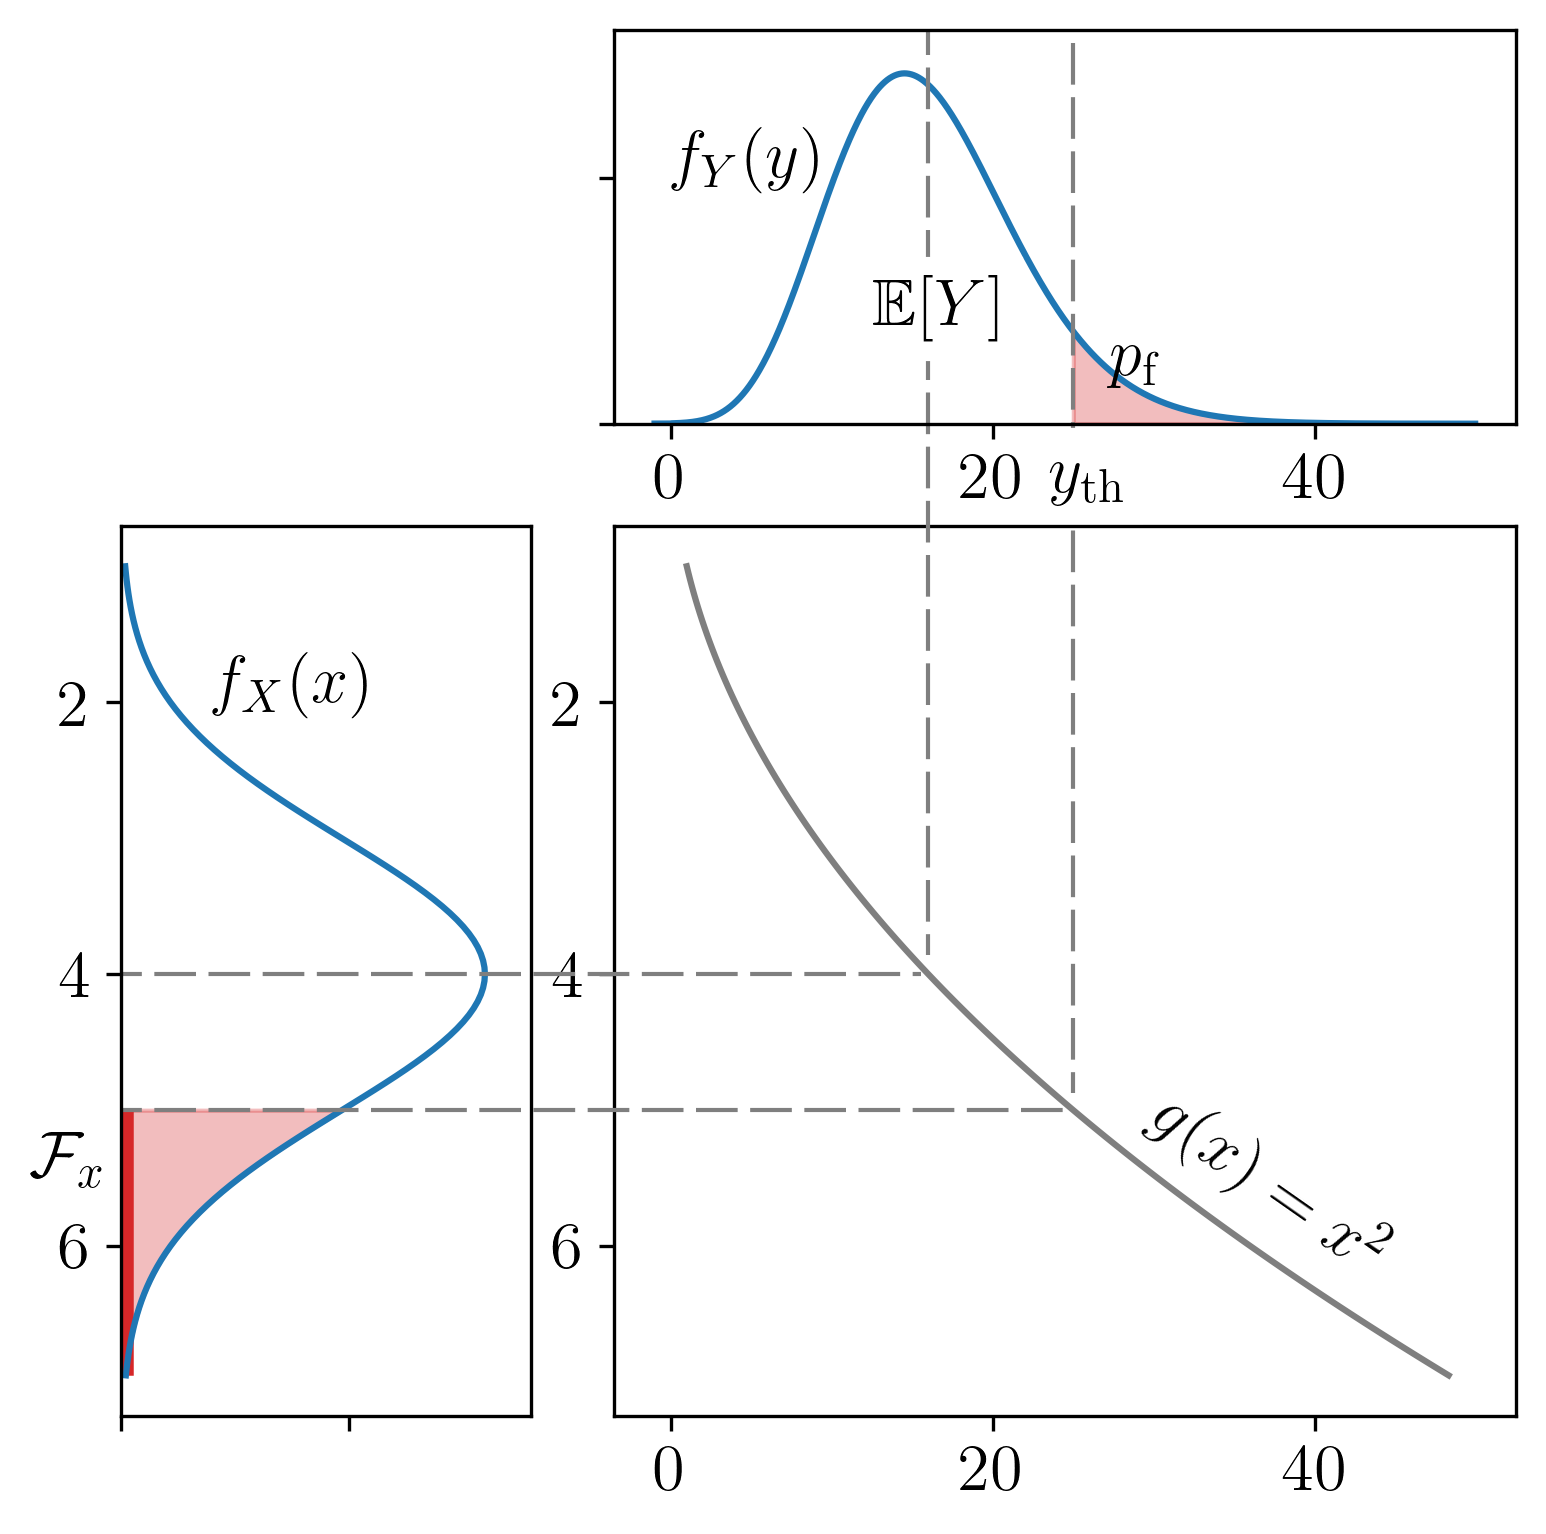
\includegraphics[width=0.5\textwidth]{../numerical_experiments/chapter1/figures/1D_reliability.png}
    \caption{One-dimensional reliability analysis example}
    \label{fig:1D_reliability}
\end{figure}

In the following, the formalism for reliability analysis problems will be first presented, 
then the main methods solving this specific problem will be introduced.
Note that the present work will not address the problems of time-dependent reliability analysis tackled in \citet{hawchar_2017}. 

%============================================================%
\subsection{Problem formalization}
%============================================================%

Following to the UQ methodology, the behavior of the system is modeled by $\iM(\cdot)$. 
Considering the problem of exceeding a safety threshold in \elias{add ref}, the system's performance is commonly defined as the difference between the model's output and a safety threshold $\yth\in\R$. 
Formally, the \textit{limit-state function} (LSF) is a deterministic function $g:\R\rightarrow\R$ quantifying this performance: 
\begin{equation}
    g(\bx) = \yth - \iM(\bx).
\end{equation}
Depending on the sign of its images, this function splits the inputs space into two disjoint and complementary domains called  
the \textit{failure domain} $\iF_{\bx}$, and the \textit{safe domain} $\mathcal{S}_\bx$ which are defined as:
\begin{equation}
    \iF_{\bx} = \{\bx \in \iD_\bx \, | \,  g(\bx) \leq \yth\}, \qquad 
    \mathcal{S}_\bx := \{\bx \in \iD_\bx \, | \, g(\bx) > \yth\}. 
    %\iD_\bx = \iF_{\bx} \cup \mathcal{S}_\bx 
\end{equation}
The border between these two domains is a hypersurface called \textit{limit-state surface} (LLS), defined by $\iF_{\bx}^0 := \{\bx \in \iD_\bx | g(\bx) = 0\}$.
Similarly to any UQ study around a numerical model, this problem ca require to be resolved using a limited numbers of calls to a black-box simulator.
The difficulties of a reliability problem might come from the properties of the LSF: nonlinear, costly to evaluate or with a multimodal failure domain. 
Additionally, note that the reliability problem can be the composition of multiple reliability problems, often modeled as system of problems in series and parallel.

A rare event estimation results from a particular uncertainty propagation through the LSF. 
Considering the resulting output variable of interest $g(\bX)$, its probability of being negative (i.e., in the failure domain) is a common risk measure \elias{add pointer}.
The commonly named \textit{failure probability}, denoted $\pf$, will be our quantity of interest in reliability analysis.
This quantity is formally written\footnote{Note that this probabilistic integration is usually written using the PDF $f_\bX(\cdot)$ 
but it could identically be expressed in terms of probability measure by taking $f_\bX(\bx) \, \dd\bx = \dd \mu(\bx), \, \forall \bx \in \iD_\bx$.}: 
\begin{equation}
    \begin{split}
        \pf := \P(Y \geq \yth) &= \P(g(\bX) \leq 0)\\
        &= \int_{\iF_\bx} f_\bX(\bx) \, \dd\bx
        = \int_{\iD_\bx} \1_{\iF_\bx}(\bx) f_\bX(\bx) \, \dd\bx,
    \end{split}
\end{equation}
were the indicator function applied to the failure domain returns $\1_{\left\{\iF_{\bX}\right\}}(x) = 1$ if $x \in \iF_{\bX}$ and $\1_{\left\{\iF_{\bX}\right\}}(x) = 0$ otherwise.
Rare event estimation implies both contour finding (i.e., characterizing the LSF) and an estimation strategy targeting the failure domain (often with a limited number of simulations).
Note that failure event are qualified as rare when its failure probability has an order of magnitude between $10^{-2} \leq \pf \leq 10^{-9}$ \elias{lemaire 2009}.

Instead of directly performing a reliability analysis in the physical space (i.e., $\bx$-space), these problems are usually solved in the \emph{standard normal space} (i.e., $\bu$-space).
Worsting in the standard space reduces numerical issues potentially caused by unscaled or asymmetric marginals. 
Moreover, a larger panel of methods can be applied in the standard space since the random inputs are independent.   
The bijective mapping between these two spaces is called an ``iso-probabilistic transformation'', 
denoted $T: \iD_{\bx} \subseteq \R^d \rightarrow \R^d, \bx \mapsto T(\bX) = \bu = \left(u_1, \dots, u_d\right)\TT$. 
When considering any random vector $\bX = \left(X_1, \dots, X_d\right)\TT$ and the independent standard Gaussian vector $\bU = \left(U_1, \dots, u_d\right)\TT$, the following equalities hold:
\begin{equation}
    \bU = T(\bX) \Leftrightarrow \bX = T^{-1}(\bU).
\end{equation} 

A reliability problem can be expressed in the standard normal space. 
Let us first consider the transformed limit-state function $\check{g}$ defined as: 
\begin{equation}
    \cg : \bigg|
    \begin{array}{rcl}
        \R^d & \longrightarrow & \R\\
        \bu & \longmapsto & \check{g}(\bu) = \left(g \circ T^{-1}\right)(\bu).
    \end{array}
\end{equation}

Since this transformation is a diffeomorphism\footnote{Considering two manifolds $A$ and $B$, a transformation $T: A \rightarrow B$ is called a diffeomorphism if it is a differentiable bijection with a differentiable inverse $T^{-1} : B \rightarrow A$.}, 
one can apply the change of variable $\bx = T(\bu)$ to express the realibility problem from \elias{add pointer} in the standard space: 
\begin{equation}
    \pf = \P(\cg(\bU) \leq 0) 
        = \int_{\iF_\bu} \varphi_d(\bu) \, \dd\bu 
        = \int_{\R^d} \1_{\iF_\bu}(\bu) \varphi_d(\bu) \, \dd\bu,
\end{equation}
with the transformed failure domain noted $\iF_\bu = \{\bu \in \R^d \, | \, \cg(\bu) \leq 0\}$, 
and the $d$-dimensional standard Gaussian PDF $\varphi_d(\bu) = \frac{1}{(2\pi)^{d/2}} \exp\left(-\frac{\lVert\bu\rVert^2_2}{2}\right)$. 
The fact that the failure probability is invariant by this transformation allows the analyst to estimate this quantity in both spaces.  

Different types of transformations exist, such as the Rosenblatt or the generalized Nataf transformation \citep{Lebrun_PHD_2013}
In practice, the transformation choice depends on the properties of the input distribution studied. 
\elias{When should we use what? In this case the distribution is not elliptical so the default method is the Rosenblatt transform.}



%============================================================%
\subsection{Rare event estimation methods}
%============================================================%
%\elias{Why are the previous sampling methods not suited for rare events?}
%\elias{Surrogate based methods can help the contour finding step.}

The main risk measure chosen for rare event estimation in this work is the previously introduced failure probability.
Therefore, let us recall that the goal is to build an efficient estimation (or approximation) of the following $d$-dimensional integral: 
\begin{equation}
    \pf = \int_{\iD_\bx} \1_{\iF_\bx}(\bx) f_\bX(\bx) \, \dd\bx
\end{equation}

In the context of rare event estimation using costly to evaluate numerical models, the simulation budget is often limited to $n$ runs with $\pf \ll \frac1n$. 
Which explains the need for specific methods offering approximations or simulations targeting the unknown failure domain. 
Two types of rare event estimation methods are classically presented: first, using approximation approaches, second, using sampling techniques. 
This section introduced the commonly used rare event methods, see \cite{MorioBalesdent2015} for a more exhaustive review.


%------------------------------------------------------------%
\subsubsection{First and second order reliability methods (FORM/SORM)}
%------------------------------------------------------------%

The so-called First and second order reliability methods (FORM and SORM) both rely on a geometric approximation to estimate a failure probability.
They extrapolate a local approximation of the LSF built in the vicinity of a \textit{most-probable-failure-point} (MPFP), also called \textit{design point}.
\elias{add some refs}


Working in the standard space, the methods first look for this MPFP, denoted $P^*$, with coordonates $\bu^*$, 
To find it, one can solve the following quadratic optimization problem: 
\begin{equation}
    \bu^* = \argmax_{\bu \in \R^d} \left(\1_{\iF_\bu}(\bu) \varphi_d(\bu)\right).
\end{equation}
Using the properties of the standard space allows us to rewrite it as: 
\begin{align}
    \bu^* &= \argmax_{\bu \in \R^d} \, \frac{1}{(2\pi)^{d/2}} \exp\left(-\frac{\bu\TT \bu }{2} \right) \qquad \mathrm{s.t.} \quad \bu \in \iF_{\bu}\\
          &= \argmin_{\bu \in \R^d} \, \bu\TT \bu \qquad \mathrm{s.t.} \quad \cg(\bu) \leq 0.
\end{align}
This problem becomes a quadratic optimization under nonlinear constraint. 
It is classically solved by gradient decent algorithms (e.g., AbdoRackwitz algorithm \elias{add ref}) but can also use gradient-free techniques (e.g., Cobyla algorithm \elias{add ref}).
This point (assuming that it is unique) defines the smallest Euclidian distance between the LSS and the origin of the standard space.
To understand its role in the reliability problem, let us recall that the density of the standard normal present an exponential decay in its radial and tangential direction.
Then, $P^*$ is the point with the biggest contribution to the failure probability \elias{pointer}. 

This distance between the origin and $P^*$ is a different risk measure, introduced as the \textit{Hasofer-Lind reliability index} \elias{add ref}, $\beta \in \R$ such that:
\begin{equation}
    \beta = \Vert \bu^* \Vert_2 = \balpha \TT \bu^*, \qquad \mathrm{s.t.} \quad
        \balpha = \frac{\nabla_{\bu} \,  \cg(\bu)}{\Vert \nabla_{\bu} \,  \cg(\bu) \Vert_2}.      
    %= \min_{\cg(\bu)=0} \left(sqrt{\bu\TT\bu}\right)
\end{equation}
The vector $\balpha$ is the unit vector pointing at $P^*$ from the origin point. 

Then, FORM aims at approximating the limit-state function $\cg(\cdot)$ by its first-order Taylor expansion around the MPFP, denoted $\cg_1(\bu^*)$: 
\begin{equation}
    \begin{split}
        \cg(\bu) &= \cg_1(\bu^*) + o\left(\Vert \bu - \bu^* \Vert_2^2\right)\\
                 &= \cancel{\cg(\bu^*)} + \nabla_{\bu} \,  \cg(\bu^*)\TT \left(\bu -\bu^* \right) + o\left(\Vert \bu - \bu^* \Vert_2^2\right)\\
                 &= \Vert \nabla_{\bu} \, \cg(\bu) \Vert_2 \left(\balpha\TT \bu^* - \balpha\TT \bu \right) + o\left(\Vert \bu - \bu^* \Vert_2^2\right)
    \end{split}    
\end{equation}
 
Using $\cg_1(\cdot)$ as approximation of the LSF, the failure probability can be approximated as: 
\begin{equation}
    \pf \approx \pf^{\mathrm{FORM}} = \P\left(- \balpha\TT \bu \leq -\beta\right) = \Phi(-\beta),
\end{equation} 
with $\Phi(\cdot)$ the CDF of the standard Gaussian. 
Depending on the properties of the LFS, this approximation will be more or less accurate. 
Note that for a linear LFS, $\pf = \pf^{\mathrm{FORM}}$. 
When the function is nonlinear, adding a quadratic term to the Taylor expansion can help the approximation. 
The approximation method is then called SORM for \textit{second order reliability method}. 
However, this added complexity implies the computation of Hessian matrices, which can be complicated (see \elias{Bourinet Chap. 1 for their estimation}).


\begin{figure}[ht]
    \centering
    \begin{subfigure}[b]{0.32\textwidth}
        \centering
        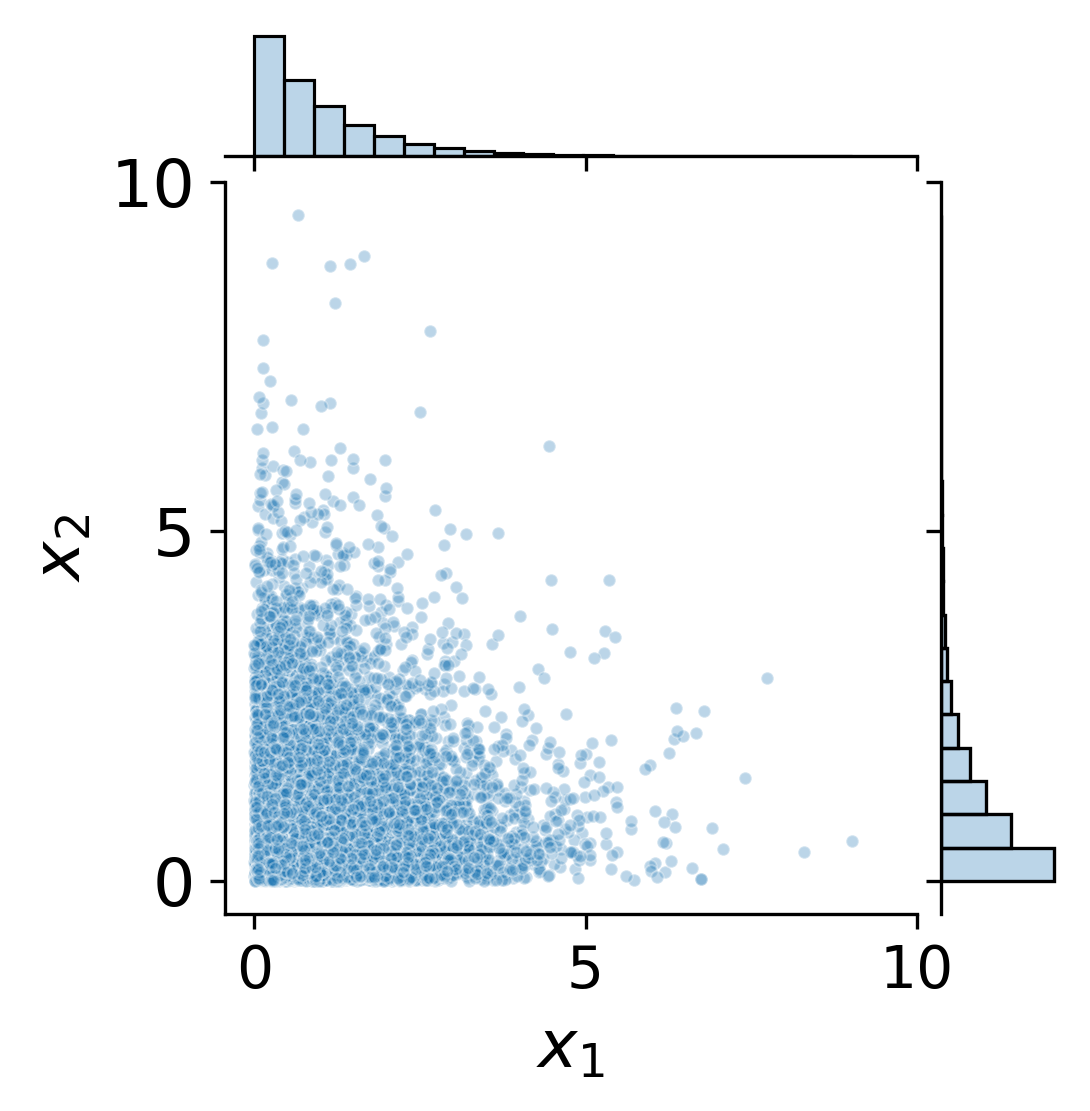
\includegraphics[width=\textwidth, draft]{../numerical_experiments/chapter1/figures/independent_copula.png}
        \caption{FORM approximation}
    \end{subfigure}
    \quad
    \begin{subfigure}[b]{0.32\textwidth}
        \centering
        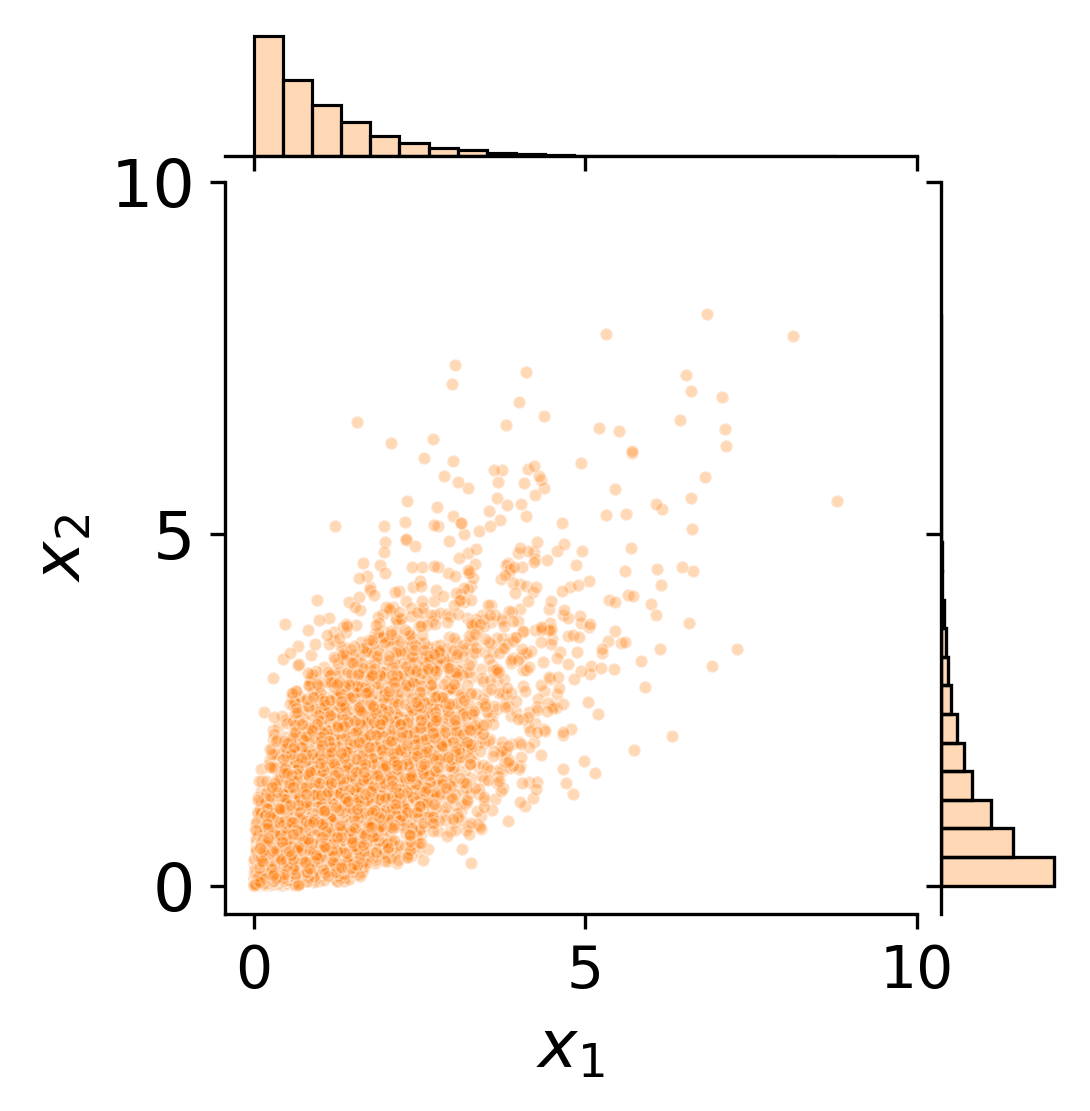
\includegraphics[width=\textwidth, draft]{../numerical_experiments/chapter1/figures/normal_copula.png}
        \caption{SORM approximation}
    \end{subfigure}
       \caption{FORM and SORM approximation on a two-dimensional example}
       \label{fig:FORM_SORM_approx}
\end{figure}


When the MPFP is not unique, the application of these methods might lead to important errors.
From a geometrical point of view, having more than one MPFP means that more than one failure zones are at the same euclidean distance of the origin.
Applying a FORM or SORM resolution in this particular case leads to the estimation of only one of the failure zones.
The \textit{muti-FORM} algorithm developed by \elias{add ref} prevents this situation by applying successive FORM. 
Once the first MPFP $P^{*^{(1)}}$ found, the LSS is modified by removing a nudge to find to following MPFP $P^{*^{(2)}}$. 

\begin{figure}[ht]
    \centering
    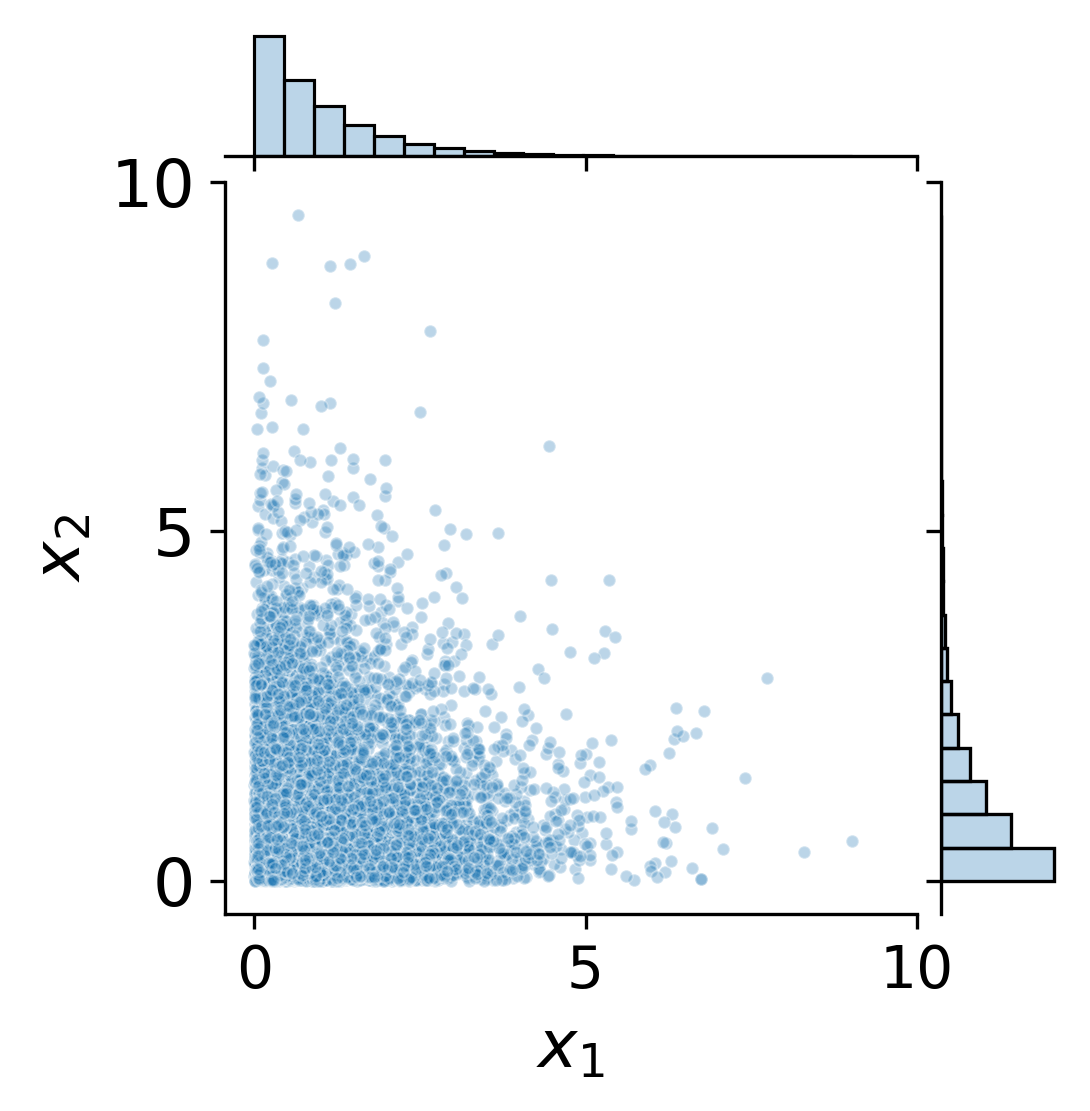
\includegraphics[width=0.32\textwidth, draft]{../numerical_experiments/chapter1/figures/independent_copula.png}
    \caption{Multi-FORM approximation on an example with two MPFPs}
    \label{fig:multi_FORM}
\end{figure}

%FORM/SORM first looks for an appropriate approximation of the limit state surface by a simple hypersurface. 
%Then, working in the standard space allows direct calculation of the failure probability considering the approximated limit state function.

Overall, FORM and SORM methods deliver a very efficient approximation of small probabilities for relatively simple problems (in terms of linearity and dimension). 
For this reason, they have been widely used in the practical context of limited simulation budget. 
However, these methods present serious limits as the dimension increases (see the discussion in \elias{Chabridon} Chapt. 1). 
Additionally, their main drawback is the lack of complementary information concerning the confidence of the results. 
The example from the \elias{Fig xx} has shown that the method might miss some important areas of the failure domain, leading to poor estimations. 
As an alternative to approximation methods, simulation-based methods often provide to the analyst an assessment of the estimation's confidence. 



%------------------------------------------------------------%
\subsubsection{Monte Carlo}
%------------------------------------------------------------%
Crude Monte Carlo sampling is a universal and empirical method for uncertainty propagation. 
As introduced earlier, it relies on the pseudo-random generation of a i.i.d. sample $\left\{\bx^{(i)}\right\}_{i=1}^n \simiid f_\bX$.   
Only the estimator is written using the indicator function with the LSF: 
\begin{equation}
    \pf \approx \what{\pf}^{\textrm{MC}} = \frac1n \sum_{i=1}^{n} \1_{\iF_\bx}(\bx^{(i)})
\end{equation} 

Provided that the failure probability is bounded, this estimator converges towards it almost surely according to the LLN. 
Once again, Monte Carlo offers a nonbaised estimator, regardless of the problem's dimension or regularity of the function $g(\cdot)$  
Additionally, the variance of this estimator is fully known:
\begin{equation}
    \var\left(\what{\pf}^{\textrm{MC}}\right) = \frac1n \pf (1 - pf)
\end{equation} 
The variance of this estimator can be used to build its confidence interval according to the TCL \elias{pointer to the previous IC}. 
Because of the small scale of the quantities manipulated in rare event estimation, the estimator's coefficient of variation is also widely used: 
\begin{equation}
    \delta_{\what{\pf}^{\textrm{MC}}} = \frac{\sqrt{\var\left(\what{\pf}^{\textrm{MC}}\right)}}{\E[\what{\pf}^{\textrm{MC}}]}
                                      = \sqrt{\frac{1 - \pf}{n \pf}}.
\end{equation}

On paper, Monte Carlo estimator presents multiple advantages for rare event estimation.
First, this method can be applied directly in the physical space, without transformation (which is practical for complex input distributions).
Second, it does not suffer from the curse of dimensionality. 
Thrid, it is qualified as embarrassingly parallel method since each numerical simulations are independent.
Finally, it offers strong convergence guaranties and complementary information on the estimation confidence.
\elias{These properties make it the reference method.}


However, these advantages of this estimator are shadowed by its slow convergence. 
To estimate a target failure probability $\pf=10^{-\alpha}$, 
a Monte Carlo estimation with a convergence level $\delta_{\what{\pf}^{\textrm{MC}}} = 0.1$ famously requires $n=10^{\alpha + 2}$ simulations. 

In the context of rare event estimation, Monte Carlo needs a number of simulation that is often prohibitive in practice. 
This excessive simulation budget comes from the fact that the vast majority of the samples drawn from the input distribution are not in the failure domain.


\newpage
%------------------------------------------------------------%
\subsubsection{Importance sampling}
%------------------------------------------------------------%

Importance sampling (IS) is a variance reduction method, aiming at improving the performances of crude Monte Carlo sampling. 
In the context of rare event estimation, the main idea is to deliberately introduce a bias in the sampled density, shifting it towards the failure domain. 
If this shift actually goes towards the failure domain, it allows to draw more points in it, leading to a better estimate of our quantity.

The challenge in importance sampling is to pick a relevant \textit{instrumental} distribution $h_\bX$ (also called \textit{auxiliary} distribution) to replace the distribution $f_\bX$. 
Then, by introducing the fully known likelihood ratio $w_\bX(\bx) = \frac{f_\bX(\bx)}{h_\bX(\bx)}$, one can rewrite $f_\bX(\bx) = w_\bX(\bx) h_\bX(\bx)$ and inject it in the failure probability expression: 
\begin{equation}
    \pf = \int_{\iD_\bx} \1_{\iF_\bx}(\bx) f_\bX(\bx) \, \dd\bx
        = \int_{\iD_\bx} \1_{\iF_\bx}(\bx) w_\bX(\bx) h_\bX(\bx) \, \dd\bx
\end{equation}
This simple writing trick allows us to integrate against the auxiliary distribution. 
With a Monte Carlo method, this task should be easier than integrating directly against the initial distribution.

The importance sampling estimator of the failure probability is defined for a sample drawn on the auxiliary distribution $\left\{\bx^{(i)}\right\}_{i=1}^n \simiid h_\bX$: 
\begin{equation}
    \what{\pf}^{\mathrm{IS}} = \frac1n \sum_{i=1}^{n} \1_{\iF_\bx}(\bx^{(i)}) w_\bX(\bx^{(i)}).
\end{equation}
This estimator is unbiased and its variance is defined as: 
\begin{equation}
    \var\left( \what{\pf}^{\mathrm{IS}}\right) = \frac1n \left( \E_{h_\bX}\left[\left(\1_{\iF_\bx}(\bX) w_\bX(\bX)\right)^2\right] - \pf^2\right).
\end{equation}
The quality of the variance reduction in this method fully depends on the choice of the instrumental distribution. 
An optimal instrumental distribution $h_{\bX}^*$ theoretically gives the smallest variance by setting it equal to zero in \elias{pointer}: 
\begin{equation}
    h_{\bX}^*(\bx) = \frac{\1_{\iF_\bx}(\bx) f_\bX(\bx)}{\pf}. 
\end{equation}
This optimal results presented in \elias{add ref} is unfortunately not usable in practice since it uses the targeted quantity $\pf$. 
Knowing this framework, various techniques try to define instrumental distributions as close as possible to this theoretical result. 
Three main importance sampling techniques are used in this work. 

\elias{First, FORM-iS}

\elias{Second AIS-CE} 

\elias{Finally, NAIS}
 
Appendix \ref{apx:C} develops an algorithmic presentation of the two last techiniques: NAIS and AIS-CE.

\elias{Discussion on commun advantages and drawback of the IS methods.}

%------------------------------------------------------------%
\subsubsection{Subset sampling}
%------------------------------------------------------------%

Subset sampling splits the failure event $\iF_{\bx}$ into an intersection of $k_\#$ intermediary events $\iF_{\bx} = \cap_{k=1}^{k_\#} \iF_{[k]}$.
Each are nested such that $\iF_{[1]} \supset \dots \supset \iF_{[k_\#]} = \iF_{\bx}$.
The failure probability is then expressed as a product of conditional probabilities:
\begin{equation}
    \pf = \P(\iF_{\bx}) = \P(\cap_{k=1}^{k_\#} \iF_{[k]}) = \prod_{k=1}^{k_\#} \P(\iF_{[k]} | \iF_{[k-1]}).
\end{equation}
From a practical point of view, the analyst tunes the algorithm by setting the intermediary probabilities $\P(\iF_{[k]} | \iF_{[k-1]}) = p_0, \forall k \in \{1, \dots, k_\# \}$. 
Then, the corresponding quantiles $q_{[1]}^{p_0} > \dots > q_{[k_\#]}^{p_0}$ are estimated for each conditional subset samples $\bX_{[k], N}$ of size $N$. 
Note that the initial quantile is estimated by crude Monte Carlo sampling on the input PDF $f_{\bX}$. 
Following conditional subset samples are generated by MCMC sampling of $f_{\bX}(\bx |\iF_{[k-1]})$, using as seeds initialisation points the $n= N p_0$ samples given by $\mathbf{A}_{[k], n}=\{\bX_{[k-1]}^{(j)} \subset \bX_{[k-1], N}| g(\bX_{[k-1]}^{(j)}) > \widehat{q}_{[k-1]}^\alpha \}_{j=1}^n$. 
This process is repeated until an intermediary quantile exceeds the threshold: $\widehat{q}_{[k_\#]}^{p_0} < \yth$. 
Finally, the failure probability is estimated by:
\begin{equation}
    \pf \approx \widehat{\pf}^{\mathrm{SS}} = p_0^{k_\# -1} \frac1N \sum_{j=1}^N \1_{\{g(\bx) \leq \yth\}} (\bX_{[k_\#],N}^{(j)}).
\end{equation}

In practice, the subset sample size should be large enough to properly estimate intermediary quantiles, which leads \cite{AuBeck2001} to recommend setting $p_0=0.1$. 
SS efficiency depends on the proper choice and tuning of the MCMC algorithm \citep{Papaioannou_PEM_2015}. 
%Our work uses the SS implementation from \texttt{OpenTURNS}\footnote{\href{https://openturns.github.io/www/index.html}{https://openturns.github.io/www/index.html}} \citep{baudin_dutfoy_2017} which integrates a component-wise Metropolis-Hastings algorithm. 
%As an alternative to generating samples on a conditional distribution by MCMC, one could try to fit this conditional distribution.





\elias{Mention the appendix Appendix \ref{apx:C} presenting the algorithms of SS}


\elias{Discussion: Which strategy to solve these problems?}



%============================================================%
%============================================================%
\section{Sensitivity analysis}
%============================================================%
%============================================================%

%============================================================%
\subsection{Global sensitivity analysis}
%============================================================%

%============================================================%
\subsection{Reliability-oriented sensitivity analysis}
%============================================================%





%============================================================%
%============================================================%
\section{Metamodeling}
%============================================================%
%============================================================%
Note that the calibration error is often larger than the metamodeling error.

%============================================================%
\subsection{Global metamodel}
%============================================================%

%============================================================%
\subsection{Contour finding for rare-event estimation}
%============================================================%






%============================================================%
%============================================================%
\section{Conclusion}
%============================================================%
%============================================================%

%!TEX root = ../thesis.tex
%*******************************************************************************
%*********************************** Second Chapter *****************************
%*******************************************************************************
\cleardoublepage
\chapter{Introduction to wind turbine modeling and design}
\label{chpt:2}
%*******************************************************************************
\hfill
\localtableofcontents
\newpage



%https://eolienne.f4jr.org/eolienne_etude_theorique

%https://www.geotechnique-journal.org/articles/geotech/pdf/2018/04/geotech190004s.pdf

%https://en.wikipedia.org/wiki/Wind-turbine_aerodynamics

%@book{hansen2015aerodynamics,
%  title={Aerodynamics of wind turbines},
%  author={Hansen, Martin OL},
%  year={2015},
%  publisher={Routledge}
%}

%============================================================%
%============================================================%
\section{Introduction}
%============================================================%
%============================================================%

Wind energy is a highly competitive industry with increasing regulations regarding its impact on ecosystems, land and sea-use, landscapes, or air traffic management \citep{eolien_en_mer_2022}. 
During the long process to win calls for tenders, obtain construction permits, or through the wind farm exploitation, an advanced technical understanding of such systems might offer a competitive advantage. 

The operation of offshore wind turbines (OWTs) is driven by multiple physics coupled. 
This behavior results from different external solicitations which are highly turbulent and uncertain. 
Among them, the \textit{metocean} (abbreviation of ``meteorology'' and ``oceanography'') environmental conditions play a primary role. 
Yet, many other types of solicitations affect the exploitation of offshore wind turbines e.g.: the corrosion of the structure, global scour, marine growth, stress concentration factor induced by the manufacturing quality, etc. 

In this context, numerical models have been developed to certify the structural integrity of OWTs with respect to their solicitations. 
A wind farm project planned at given location should pass different validation procedures established by international standards such as the International Electrotechnical Commission \citep{iec_2019}. 
As wind turbine structures face a large amount of stress cycles in their lifetime (up to $10^8$ for 20 years of operation), this chapter will particularly focus on fatigue damage assessment.

The present thesis studied different steps of uncertainty quantification on two wind farm projects. 
First the Teesside wind farm, operating since 2014 in the North Sea, second the theoretical wind farm of south Brittany, currently at the stage of calls for tenders.

Considering the standard uncertainty quantification diagram presented in \fig{fig:UQ_methodo}, the material of this chapter is related to the step A (problem specification) and the step B (uncertainty quantification). 
It briefly introduces wind turbine modeling and design, in the following layout: 
Section \ref{sec:metocean_simulation} presents the methods used for wind and wave generation and wake simulation at a farm scale; 
Section \ref{sec:owt_modeling} recalls elements of theory associated with wind turbine modeling; 
Section \ref{sec:owt_design} introduces recommended practices regarding design and operation; 
finally, Section \ref{sec:owt_uncertainties} gives a description of the various sources of uncertainties considered in this thesis. 
%To go further this general introduction, the reader might refer to the following sources on the different topics 



%============================================================%
%============================================================%
\section{Metocean conditions simulation} \label{sec:metocean_simulation}
%============================================================%
%============================================================%

In the atmosphere, the wind represents the air movements caused by the heterogeneous solar heating of Earth's surface. 
Winds usually move from high-pressure to low-pressure regions. 
Earth's rotation also impacts large-scale climate patterns, including winds by the intermediate of the well-known Coriolis effect. 
The wind is a highly variable resource, making its exploitation for energy production uncertain. 
This variability is both expressed in space and time with different behaviors depending on the scales studied. 

Regarding large timescales, yearly seasonal fluctuations of wind conditions are well-defined using probability distributions (typically Weibull distributions). 
However, predictions at a shorter timescale are usually unreliable beyond a few days ahead. 
Under a few days, the spectral wind energy distribution per time unit is represented by its power spectral density (PSD). 
Historically, the spectral study of horizontal wind by \citet{van_1957_wind_psd} for timescales between a few seconds and ten days revealed distinct ranges of behaviors. 
The PSD, such as the one illustrated in \fig{fig:wind_psd}, presents three main separated peaks, explaining how the wind energy is split. 
The two first peaks are named ``synoptic'' and ``diurnal'' peak, which respectively correspond to return periods around four days and one day. 
While these two peaks are relatively close together, the third peak is completely separated. 
This third peak describes the energy related to wind turbulence, which evolves in a range below ten minutes. 
Considering this typical energy distribution, wind behaviors are often referred to as ``short-term'' (for turbulent wind) and ``long-term'' (otherwise). 
In wind turbine simulation, ten minutes simulations became a common practice to fully consider turbulent winds. 

Remark that the spectrum presented in the research paper of \citet{van_1957_wind_psd} (represented in \fig{fig:wind_psd}) was build from wind measures near New York, USA. 
The same pattern between the three peaks is rather constant between sites, however, the geography (including the surface roughness, the topology, the proximity to the coast, etc.) may affect this distribution. 

At a larger timescale than one year, assessing trends becomes more complicated. 
Additionally, wind resource assessment over decades is made more uncertain by climate change \cite{nagababu_2023_climate_change}, disrupting large weather trends and increasing the occurrence of extreme events. 

\begin{figure}
    \centering
    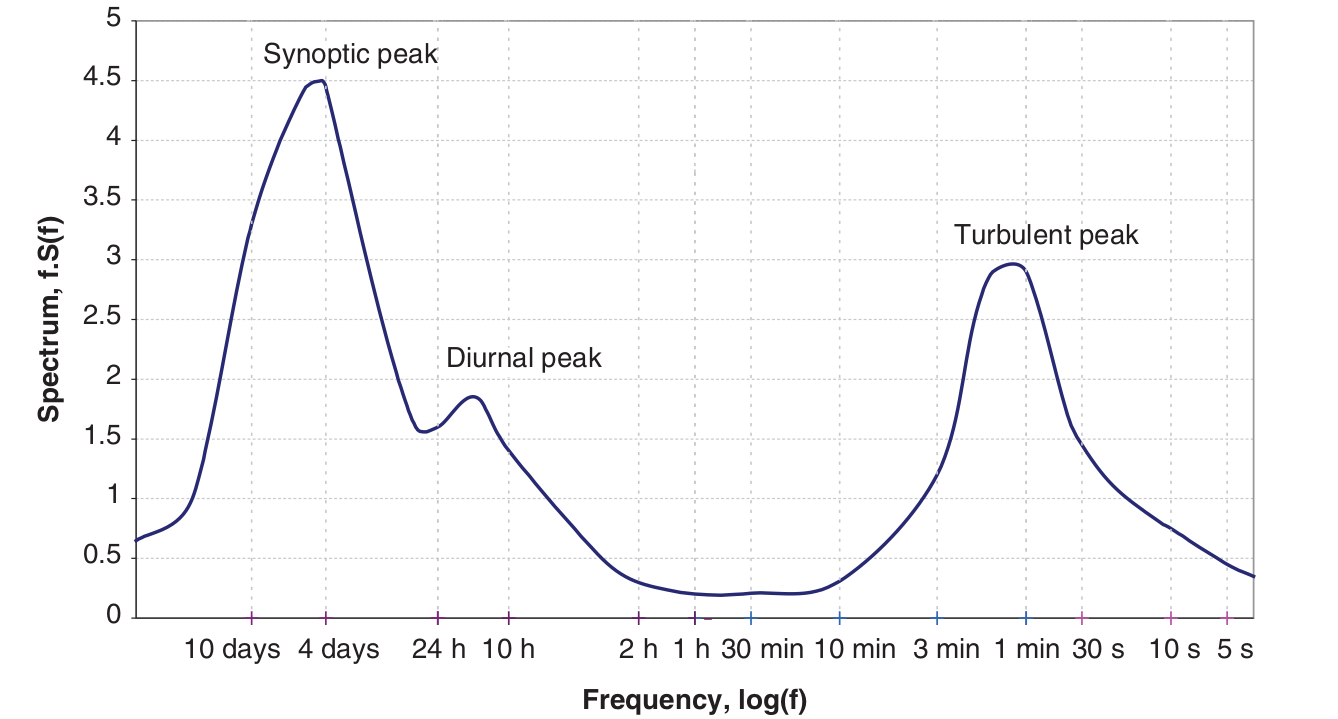
\includegraphics[width=0.7\textwidth]{./part1/figures/wind_spectrum.png}
    \caption{Wind spectrum from Brookhaven, USA (source: \citealt{burton_2021_wind_handbook})}
    \label{fig:wind_psd}
\end{figure}

%\elias{Add something general regrading wave modeling?}



%============================================================%
\subsection{Turbulent wind generation}\label{sec:221}
%============================================================%

Wind turbulence is a complex and aleatory process, often described as chaotic, since a small perturbation of its initial conditions might have an important impact on the response. 
However, the wind over short-term periods (i.e., ten minutes periods) is usually assumed to be a Gaussian process with constant mean $\overline{U}$ and standard deviation $\sigma_U$ \citep{burton_2021_wind_handbook}. 
Its mean is modeled by the long-term wind conditions (i.e., mean wind speed), often described by a probabilistic model such as a Weibull distribution. 
\elias{This short-term / long-term modeling hypothesis is represented in \fig{fig:wind_long_short_term}.} 
Note that this assumption is based on the bimodal wind energy distribution observed in \fig{fig:wind_psd}, which might vary at some specific locations. 

The \textit{turbulence intensity} is a commonly used normalized statistic of the wind variability: 
\begin{equation}
    I = \frac{\sigma_U}{\overline{U}}.
\end{equation}

\begin{figure}
    \centering
    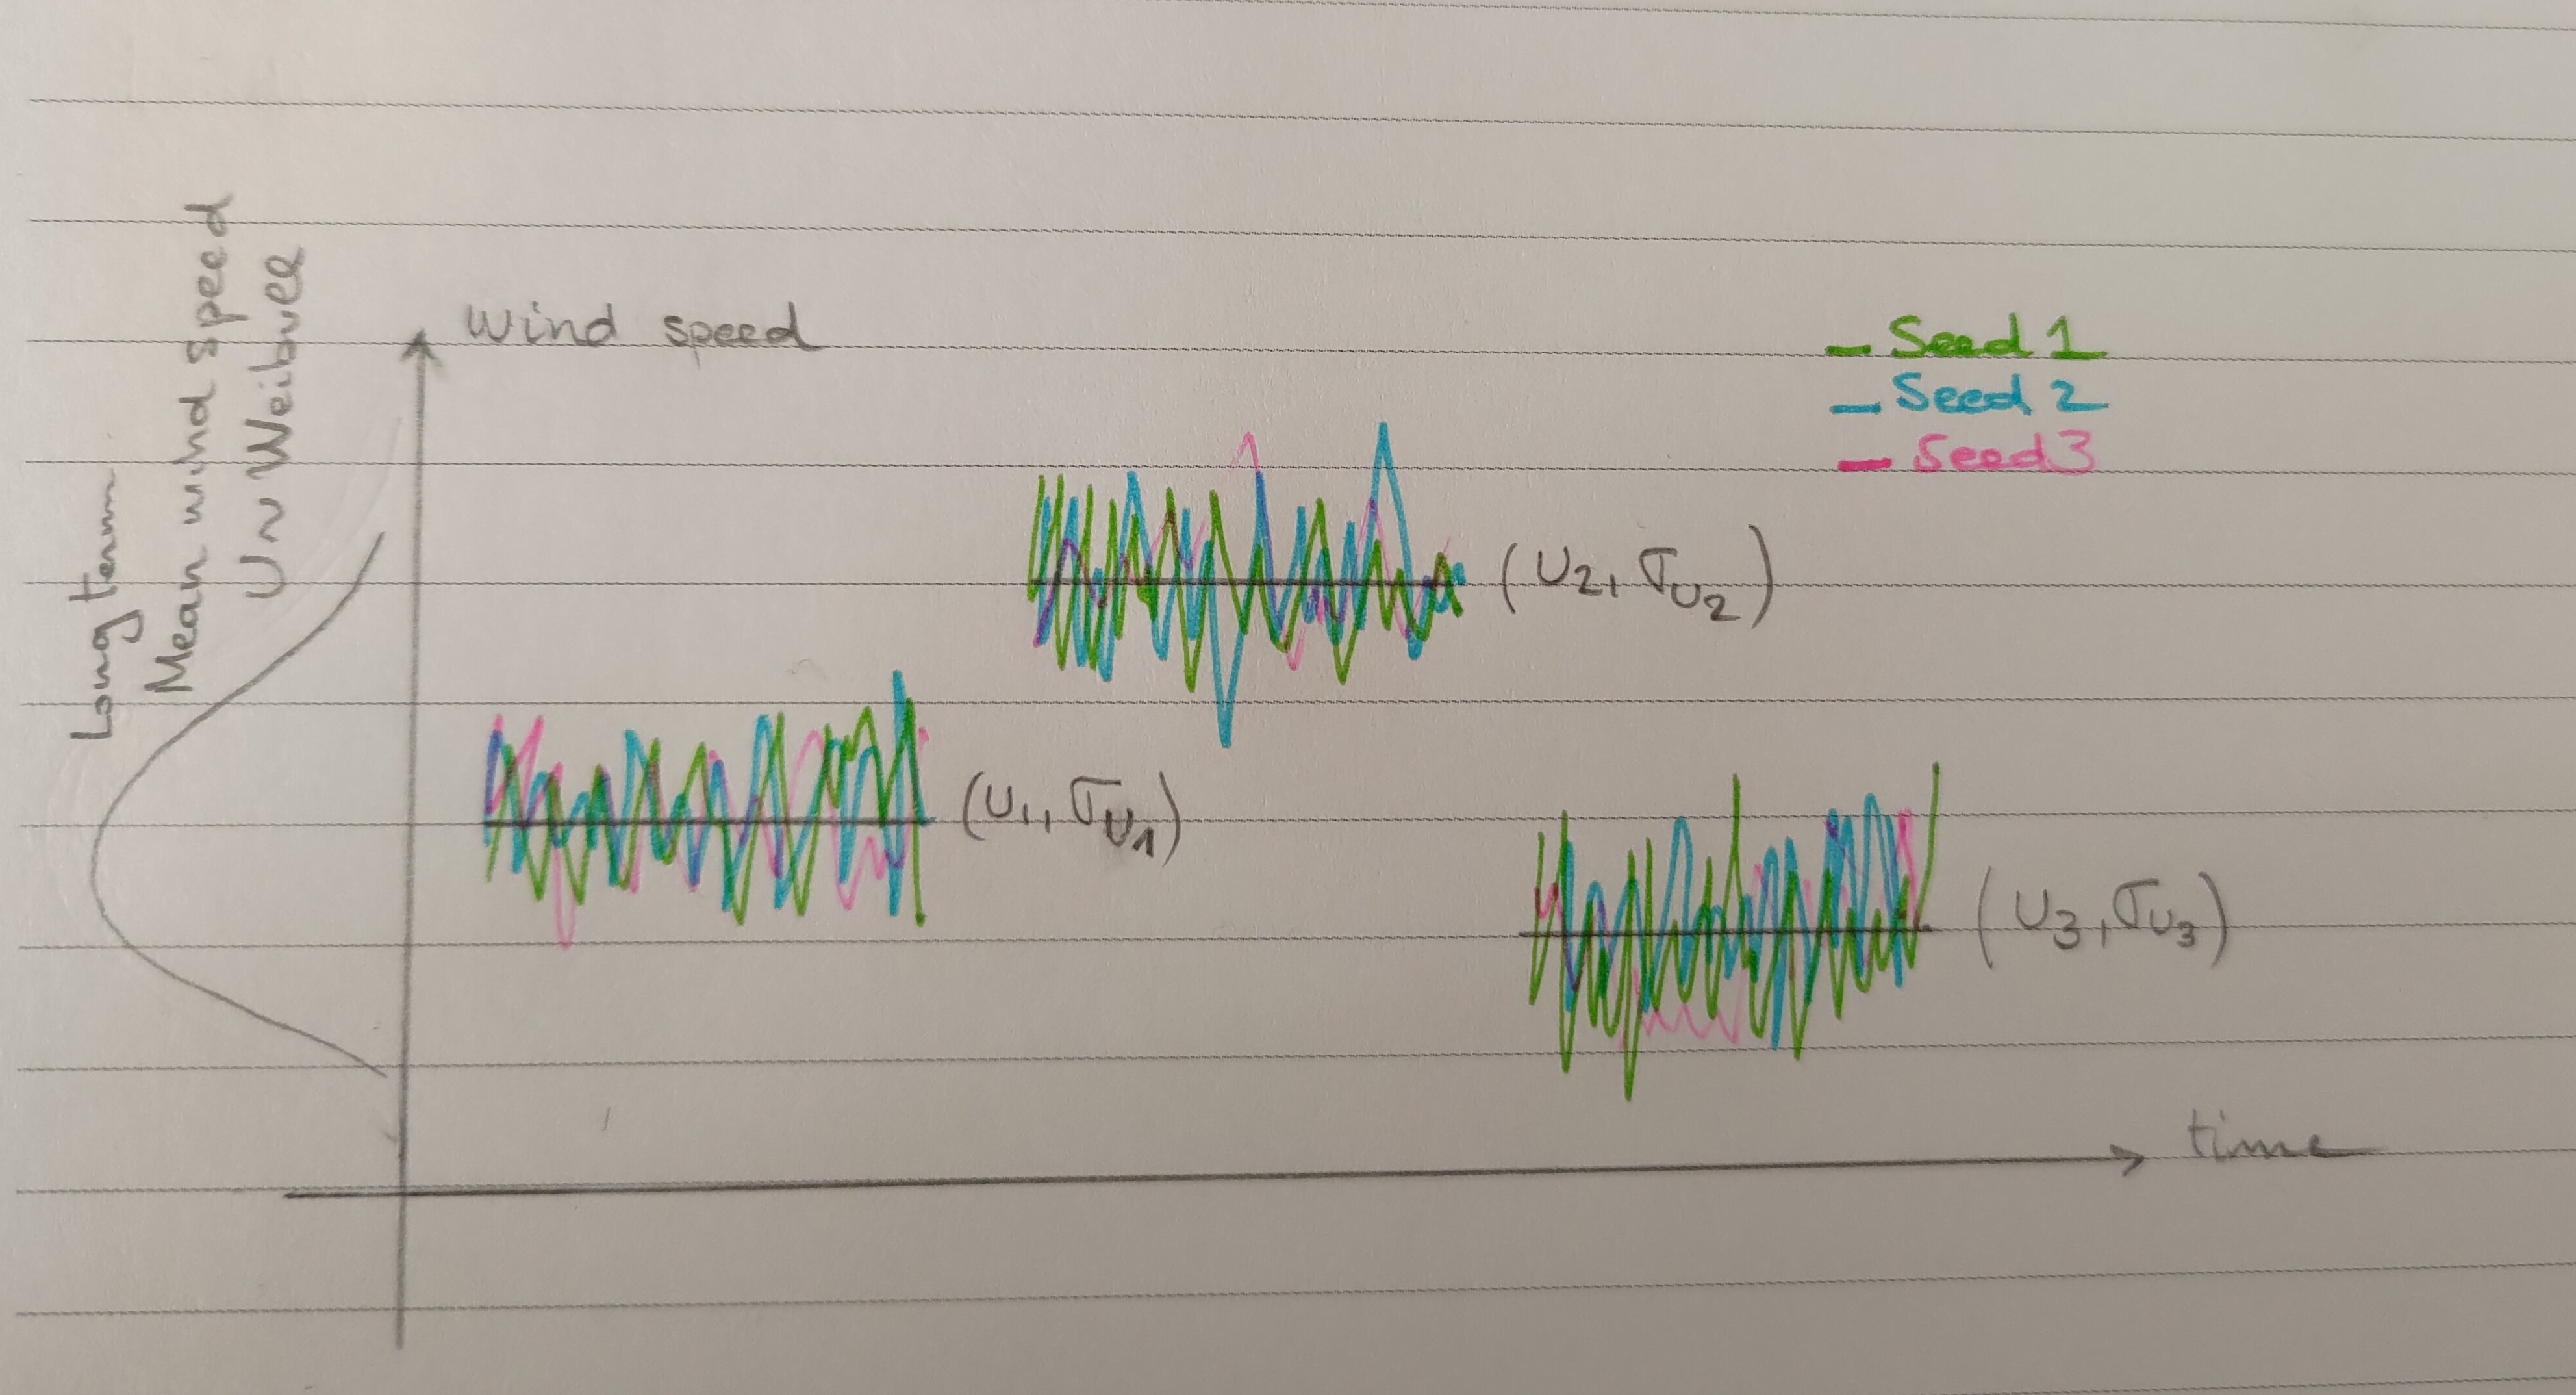
\includegraphics[width=0.7\textwidth]{./part1/figures/wind_long_short_term.jpg}
    \label{fig:wind_long_short_term}
    \caption{\elias{Should we keep this representation? If so, it will be done properly.}}
\end{figure}

As the wind depends on differences between pressure, humidity, air density, different models exist to represent vertical wind profiles. 
The vertical change in wind conditions is referred to as \textit{vertical wind shear}. 
Assuming a constant standard deviation over the altitude, the power law is a widely used model to approximate vertical shear \citep{iec_2019}:
\begin{equation}
    \overline{U}(z) = \overline{U}_0 \left(\frac{z}{z_{\mathrm{0}}}\right)^\alpha,
\end{equation}
with $\overline{U}_0$ a well-defined mean wind speed at the height $z_{\mathrm{0}}$ (typically corresponding to a measurement height), 
$z$ the studied height (e.g., the turbine's hub-height), and $\alpha$ the vertical shear coefficient (defined according to measures or standards' recommendations). 

To generate a turbulent wind field on a mesh around the turbine, the general mechanism is to apply inverse Fourier transforms on a turbulent wind spectrum.  
Two types of parametric spectrums are commonly used in wind energy: the \textit{Kaimal model} \citep{kaimal_1972} and the \textit{Mann model} \citep{mann_1998}. 
In this thesis, the Kaimal spectrum as defined in \cite{iec_2019} is used for turbulent wind generation over the Cartesian component $k \in \{u, v, w\}$:
\begin{equation}
    S_k(f) = \frac{4 \sigma_k^2 \frac{L_k}{\overline{U}}}{\left(1 + 6 f \frac{L_k}{\overline{U}}\right)^{5/3}},
    \label{eq:kaimal}
\end{equation} 
such that $f$ is the frequency, $\overline{U}$ is the longitudinal mean speed at hub-height, $L_k$ are the Kaimal length scales, and $\sigma_k$ standard deviations. 
Along with the Kaimal wind speed spectrum, a spacial coherence model is usually defined in the frequency domain. 
Each couples of nodes in the mesh are correlated, for example, using an exponential coherence model (see the complete definition in Annex C of \citealt{iec_2019}).

In this thesis, the full-field turbulent wind fields (i.e., over a regular mesh) are generated using TurbSim, a software developed by the National Renewable Energy Laboratory (NREL) \citep{turbsim_2009}. 
TurbSim generates time realizations by adapting the spectral method proposed in \citet{veers_1988_sandia} (relying on the inverse Fourier transforms of each axial component).   
Considering a wind spectrum (e.g., Kaimal model) and a vertical shear model (e.g., power law), TurbSim takes as inputs a mean wind speed, a turbulence standard deviation and a mean wind orientation. 
\fig{fig:turbsim_simu} illustrates the corresponding wind field generated by a ten-minutes TurbSim simulation, considering a set of input long-term conditions. 

\begin{figure}
    \centering
    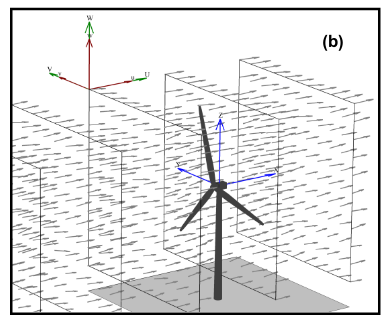
\includegraphics[width=0.5\textwidth]{./part1/figures/turbsim.png}
    \caption{Example of a turbulent wind field generated by TurbSim (source: \citealt{turbsim_2009})}
    \label{fig:turbsim_simu}
\end{figure}

In their recent review of the challenges in wind energy, \citep{veers_2019_review} list some limits of the two spectral turbulence models recommended by the standards. 
First, their parameters were fitted using a restricted amount of data \citep{dimitrov_2017_turbulence_models_on_loads}. 
Second, the spacial coherence models associated with Kaimal models showed differences with turbulence measured on site \citep{saranyasoontorn_2004}.  
Finally, recent studies showed that the choice of spectral model impacts the resulting wind turbines loads \citep{doubrawa_2019}. 
These approximations generally tend to overestimate wind flows, leading to conservative designs. 

To ensure more realistic turbulent wind field generation, two research perspectives are actively explored. 
Authors recently developed hybrid methods, including measurement data to enhance spectral models \citep{dimitrov_2017_constrained_turbulence}. 
Alternatively, higher fidelity models were studied in this domain, see for example the use of vortex methods \citep{branlard_2017_book} and large eddy simulations (LES) \citep{doubrawa_2019,bui_2022_mesoscale_LES}.  
Such complex models allow the simulation of mesoscale conditions (e.g., at the farm scale), and extreme transient events (e.g., gusts and storms). 
However, their computational cost is often prohibitive for uncertainty quantification studies. 
When studying the wind resources at a wind farm scale, modeling wind energy losses induced by the turbines' wake becomes essential. 



%============================================================%
\subsection{Wake modeling}
%============================================================%

The wake is caused by the extraction of the wind kinetic energy, reducing the wind speed and increasing the turbulence downstream of the turbines (see the illustration in \fig{fig:wake_illustration}). 
In a wind farm, this effect depends on the spacing between turbines, as well as the ambient wind speed and turbulence intensity. 
The turbines positioned at the center of the farm are indeed the most impacted by the wake. 
As a wind farm owner, the consequence of the wake is twofold: a loss of energy production (in the range of 10 to 20 percents depending on the farm), and an increase of fatigue loads (due to the asymmetric loading from the created turbulences).

\begin{figure}%[h!]
    \centering
    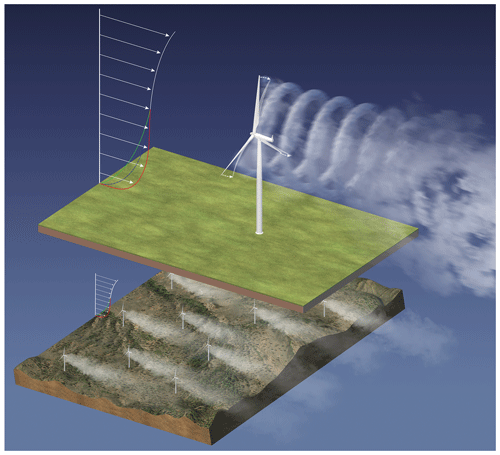
\includegraphics[width=0.5\textwidth]{./part1/figures/wake.png}
    \caption{Illustration of the wake created downstream a wind farm (source: \citealt{veers_2019_review})} 
    \label{fig:wake_illustration}
\end{figure}

The initiation of the wake is a complex physical mechanism, however, the wake almost becomes axisymmetric after two turbine diameters downstream. 
At this stage, the wind speed deficit often presents a Gaussian profile centered on the hub \citep{burton_2021_wind_handbook}. 
Numerical models of different fidelities aim at simulating the wake. 
For example, computational fluid dynamics (CFD) models give a detailed description of the wake (including near the turbine) but require high computational efforts. 
In practice, simple analytical models (often called ``engineering models'') are widely used and recommended by standards (see e.g., Annex E in \citealt{iec_2019}). 
These models mostly rely on the equivalence between the thrust load and the turbine wind energy deficit. 
Since the seminal engineering model proposed by \citet{jensen_1983_wake}, multiple enhancements were proposed. 
A wide benchmark of the wake modeling solutions for different fidelities was performed in \citet{doubrawa_2020_benchmark} and \citet{hiperwind_2023_wp3}. 
The optimal tuning of these engineering models was studied using measurements from a Doppler wind lidar in \citet{zhan_2020_optimal_wake}. 
Different software programs propose wake engineering models, such as: FLORIS (developed by the NREL \citet{fleming_2020_FLORIS}), FarmShadow (developed by IFPEN). 

To take into account the wake effect, control strategies increasingly move from the turbine scale to the farm scale. 
This concept, called ``active wake control'', introduces small yaw misalignments (making the control of turbines individually suboptimal) to optimize the global wake inside the farm \citep{rott_2018_active_control,simley_2020_active_control,meyers_2022_active_control}. 


%============================================================%
\subsection{Irregular wave generation}
%============================================================%

The propagation of wind generated waves has long been studied in hydrodynamics under the prism of different theories such as Airy's, and Stokes'. 
Airy's wave theory (also referred to as the linear wave theory) models sea states under the hypothesis of small waves relatively to the water depth.  
This spectral approach superposes many regular waves, following the same wave spectrum, to model irregular waves. 
Two standard statistics are used in oceanography to represent sea states and their corresponding wave spectra: 
the wave period $T_p$ (with the corresponding frequency $f_p$), and the significant wave height $H_s$ (average over the highest third of the waves measured). 

The most commonly used parametric wave spectrum is named JONSWAP, after the ``Joint North Sea Wave Project'' \citep{jonswap_1973}: 
\begin{equation}
    S(f) = \delta \frac{H_s^2}{f} \left(\frac{f_p}{f}\right)^4 \exp\left[-\frac54 \left(\frac{f_p}{f}\right)^4 \right] \gamma^\alpha.
    \label{eq:jonswap}
\end{equation}
The JONSWAP spectrum is a corrected version of the Pierson-Moskowitz spectrum (developed in 1964), adding a peak enhancement factor $\gamma^\alpha$. 
Further details regarding the numerical values to choose in \eq{eq:jonswap} are given in \citet{burton_2021_wind_handbook}. 
An illustration of the two spectra is presented in \fig{fig:jonswap}, revealing the enhancement factor proposed in the JONSWAP model to better fit sea states measurements. 

\begin{figure}%[h!]
    \centering
    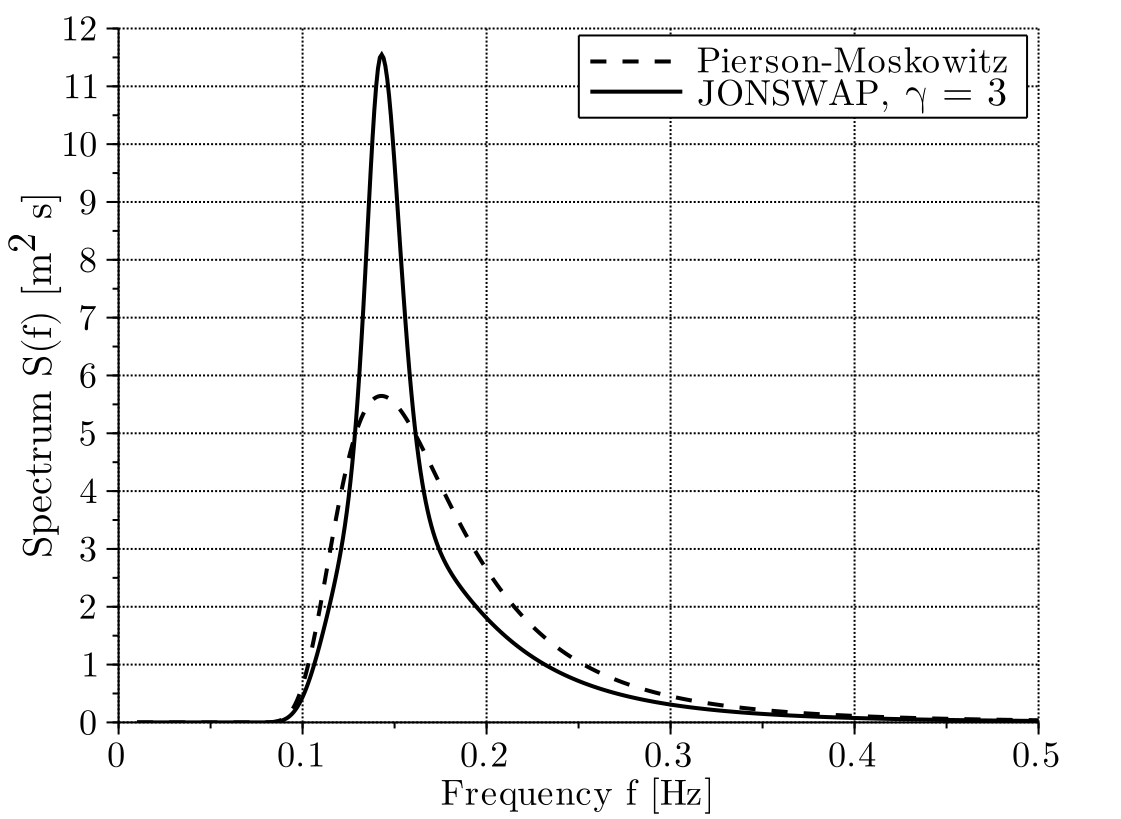
\includegraphics[width=0.45\textwidth]{./part1/figures/jonswap.png}
    \caption{Peirson-Moskowitz and JONSWAP spectra at significant wave height $H_s = 3$
    m and peak period $T_p = 7$ s (source: \citealt{milano_thesis_2021})}
    \label{fig:jonswap}
\end{figure}

Swell waves are the result of weather conditions occurring far away from the location studied. 
Such waves usually present long wavelength, allowing them to propagate over long distances with little dissipation. 
To take them into account, the unimodal wave spectra introduced in \eq{eq:jonswap} was improved. 
Different methods allow to build a parametric bimodal distribution, with a mode in the low frequencies corresponding to the swell. 
\citet{guedes_2005_bimodal_jonswap} reviews different bimodal wave spectra, and compares their adequacy with measured sea states. 



%============================================================%
%============================================================%
\section{Wind turbine multi-physics modeling} \label{sec:owt_modeling}
%============================================================%
%============================================================%

Offshore wind turbine models are coupling multiple physics such as aerodynamics, hydrodynamics, mechanical elasticity, control and mooring dynamics for floating OWT. 
Similarly to the usual practices from the offshore oil \& gas industry, OWT have been first modeled in the frequency domain. 
At an early design stage, a study in the frequency domain gives a rough idea of the system's feasibility by computing its natural frequencies. 
An OWT should not have its natural frequencies in the same range as the main frequencies of the wave energy spectra. 
Otherwise, such systems can be subject to critical dynamic resonance, leading to their failure.

Beyond this preliminary check, frequency-domain approaches present limits for OWT modeling. 
As they rely on linear assumptions, they are unable to model the nonlinearities and transient loading phases \citep{matha_2011_ISOPE}. 
These aspects happen to be essential in the design of OWTs \citep{jonkman_2011_ISOPE}. 
As an alternative, the behavior of OWT systems are also simulated in the time domain. 

In the time domain, such systems may be models for different fidelities. 
The diagram in \fig{fig:owt_modeling_fidelities} illustrates the increasing complexities for two physics involved in OWT modeling (aerodynamics and structural dynamics). 
Generally, the computational cost increases with the model fidelity, making uncertainty quantification intractable at some point. 
In the present work, the numerical model of an OWT studied is actually a chain of three models executed sequentially (as illustrated in \fig{fig:owt_chained_model}): 
\begin{itemize}
    \item \textbf{TurbSim}: a turbulent wind generator (see Section \ref{sec:221});
    \item \textbf{DIEGO}: a multiphysics wind turbine model in the time domain (see Section \ref{sec:owt_modeling}); 
    \item \textbf{Fatigue assessment}: a post-precessing computing fatigue damage (see Section \ref{sec:235}). 
\end{itemize}
DIEGO is a numerical model developed by EDF R\&D to simulate the aero-hydro-servo-elastic behavior of OWTs in the time domain. 
Different extensive code-to-code comparisons between DIEGO and other aero-hydro-servo-elastic models showed close results. 
Considering bottom-fixed OWT \citep{popko_2021_DIEGO_benchmark} or floating OWT \citep{robertson_2020_diego_benchmark,kim_natarajan_2022}, DIEGO was compared to ``FAST'' (developed by NREL), ``HAWC2'' (developed by DTU), ``BLADED'' (developed by DNV), and ``DeepLines Wind'' (developed by IFPEN). 

% Note that the wake should also be considered at the wind farm scale, as described earlier. 
\begin{figure}[h]
    \centering
    %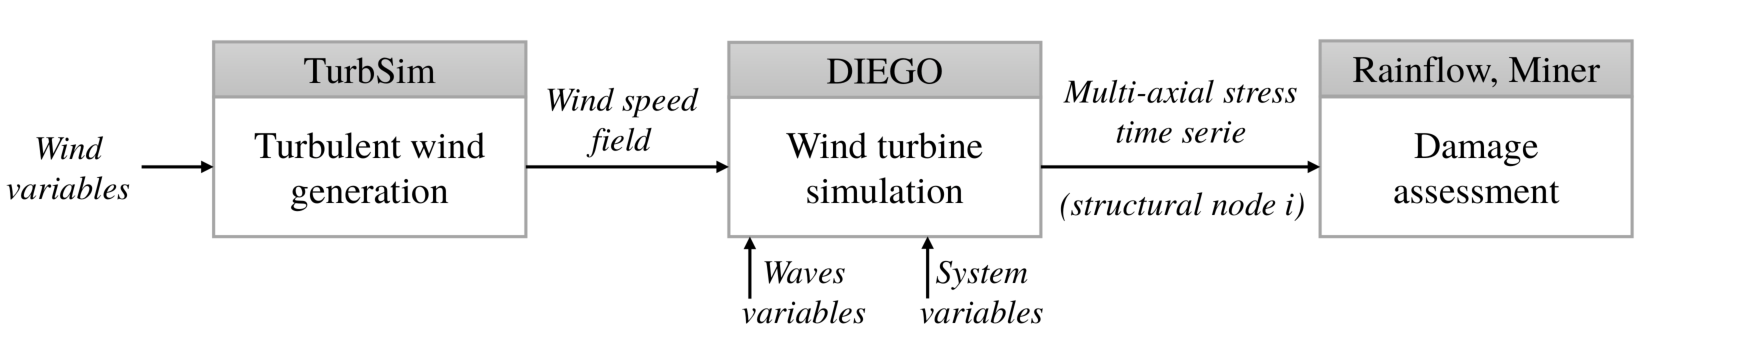
\includegraphics[width=0.8\textwidth]{./part1/figures/chained_model.pdf}
    \begin{tikzpicture}
    \node [style={grey_rect}] (0) at (0.5, 0) {Turbulent wind generation};
    \node [style={grey_rect}] (1) at (5, 0) {Wind turbine simulation};
    \node [style={grey_rect}] (2) at (9.5, 0) {Damage \\assessment};
    \node [style={grey_full_rect}] (3) at (0.5, 0.55) {TurbSim};
    \node [style={grey_full_rect}] (4) at (5, 0.55) {DIEGO};
    \node [style={grey_full_rect}] (5) at (9.5, 0.55) {Rainflow, Miner};

    \node [style=texte] (8) at (2.75, 0.3) {Wind speed\\field};
    \node [style=texte] (6) at (7.25, 0.1) {Multi-axial stress\\time series\\[3pt](structural node $i$)};
    \node [style=texte] (9) at (4.6, -1) {Wave\\variables};
    \node [style=texte] (10) at (6.2, -1) {System\\variables};
    \node (11) at (4.2, -1) {};
    \node (12) at (4.2, -0.4) {};
    \node (13) at (5.7, -1.) {};
    \node (14) at (5.7, -0.4) {};
    \draw [style=arrow] (13.center) to (14.center);
    \draw [style=arrow] (11.center) to (12.center);
    \draw [style=arrow] (1) to (2);
    \draw [style=arrow] (0) to (1);
\end{tikzpicture}
    \caption{Chained numerical model of offshore wind turbine.}
    \label{fig:owt_chained_model}
\end{figure}


\begin{figure}
    \centering
    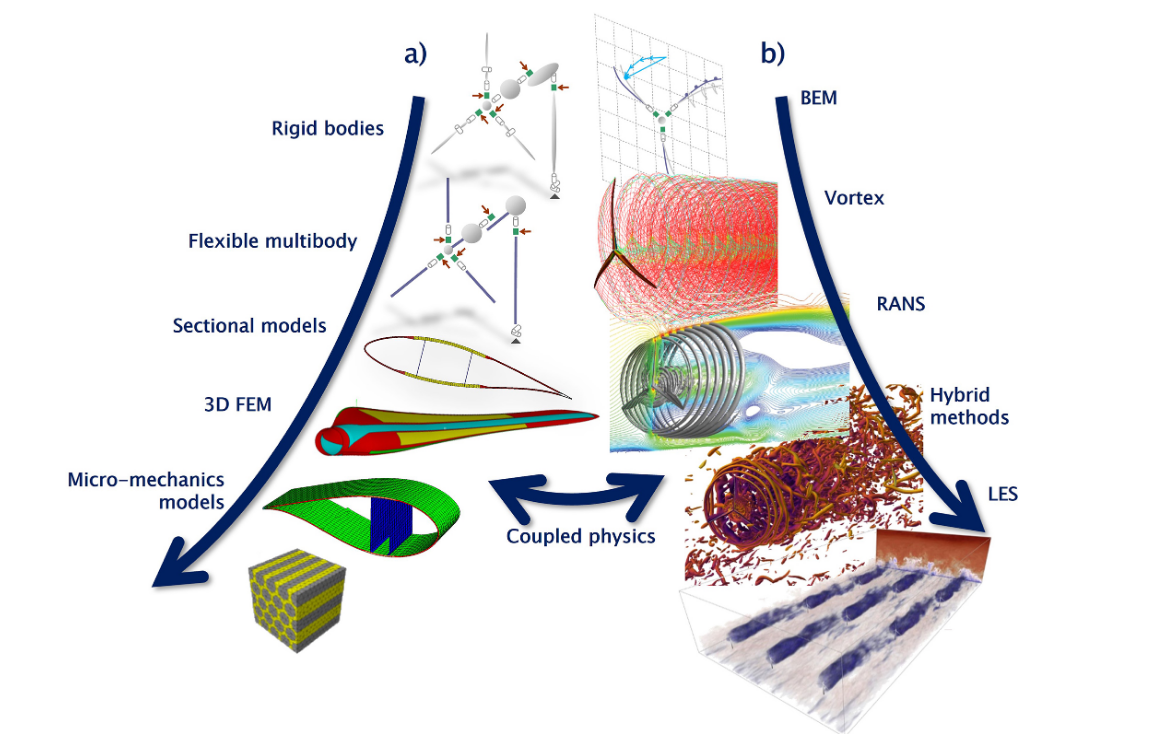
\includegraphics[width=0.7\textwidth]{./part1/figures/OWT_modeling_fidelities.png}
    \caption{Hierarchy of structural (a) and aerodynamic (b) wind energy systems models (source: \citealt{veers_2019_review})}
    \label{fig:owt_modeling_fidelities}
\end{figure}



%============================================================%
\subsection{Aerodynamics of horizontal axis wind turbines}
%============================================================%

The blade element momentum theory mixes different concepts to compute the aerodynamic forces on the rotating blades of the wind turbine. 
In this coupled physics models, the aerodynamics affects the structural response and vise-versa. 
To solve this problem, algorithms used in DIEGO first assess displacement of elementary blades, to recover the lift and drag coefficients. 
The elementary loads are then integrated over each blade and communicated to the structural model.


\paragraph{Momentum theory.}
%------------------------------------------------------------%
At the core of wind turbine's aerodynamics, the concept of \textit{momentum theory}, also called \textit{actuator disk theory} assumes that the air stream passing thought the rotor disk is bounded by a stream tube of circular surface (not mixing with the ambient air). 
\fig{fig:actuator_disk} is a longitudinal representation of the actuator disk and the way it affects the air upstream and downstream the rotor. 
The associated momentum theory assumes the conservation of airflow at any cross-section (of area $A$) during a time period. 
Passing through the actuator disk, the wind speed slows down and a drop in static pressure is at the origin of the wake. 
This pressure drop generates an axial force (called \textit{axial thrust force}) and a torque on the actuator disk.

\begin{figure}[!h]
    \centering
    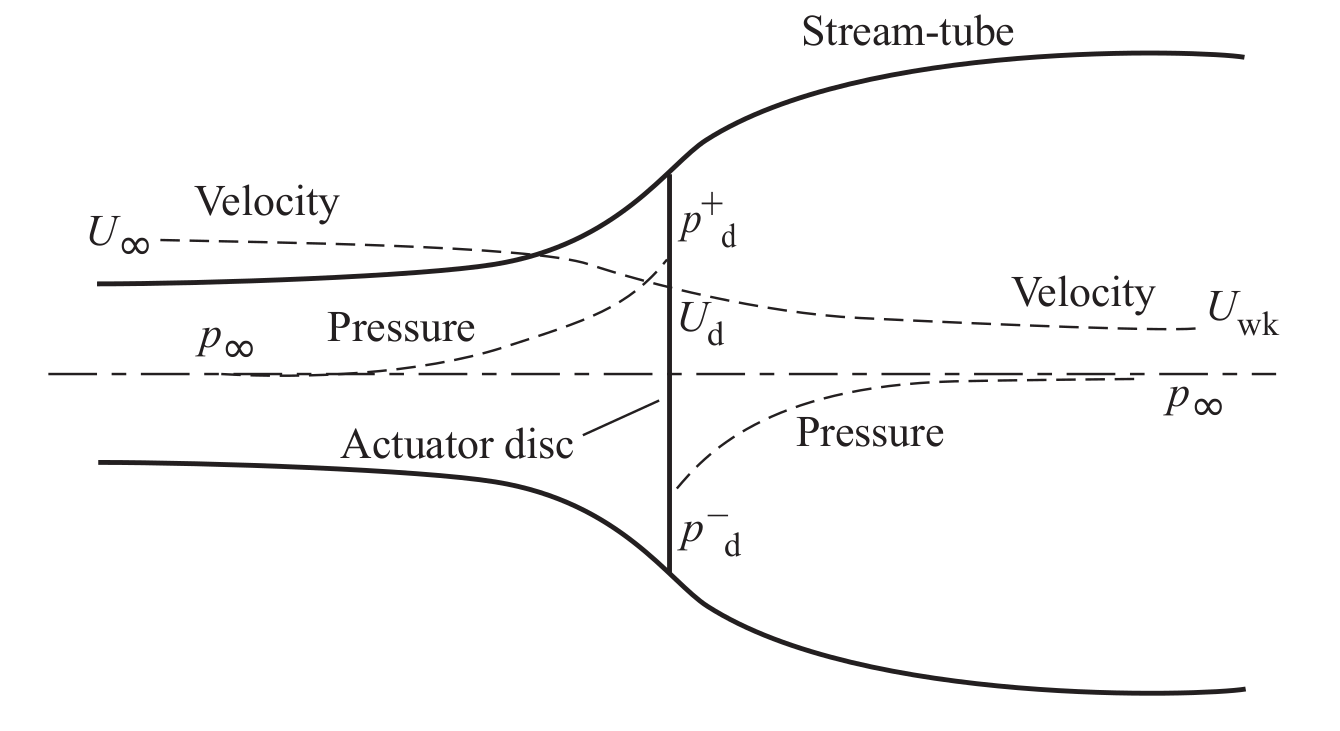
\includegraphics[width=0.6\textwidth]{./part1/figures/actuator_disk.png}
    \caption{Actuator disk model of the energy extraction (source: \citealt{burton_2021_wind_handbook}). Longitudinal evolution of the air pressure and wind speed along the wind stream.}
    \label{fig:actuator_disk}
\end{figure}
Considering the upstream flow, the flow at the rotor disk and the airflow in the wake, respectively denoted by the subscripts $\{\infty, d, \mathrm{wake}\}$, the following equality comes:  
\begin{equation}
    \rho A_\infty U_\infty = \rho A_d U_d = \rho A_{\mathrm{wake}} U_{\mathrm{wake}},
\end{equation}
where $U$ is the wind speed, $A$ the stream-tube area, and $\rho$ the air density. 
The wind speed in at the rotor disk can be expressed using the induction factor $a$ in the following expression: 
\begin{equation}
    U_d = U_\infty (1 - a), \, 0\leq a \leq 1.
\end{equation}
Using the momentum theory and Bernoulli's incompressible flow equation, one can express the aerodynamic thrust $T$ and power $P$ (see \citealt{milano_thesis_2021}): 
\begin{subequations}
    \begin{align}
        T&=(p_d^+ - p_d^-) A_d = 2 \rho A_d U_\infty^2 a (1- a)\\
        P&= T U_d = 2 \rho A_d U_\infty^3 a (1- a)^2
    \end{align}
    \label{eq:momentum_theory}
\end{subequations}
The widely used power coefficient (respectively thrust coefficient) is the ratio of the power captured by the turbine against to the total kinetic wind power available in the stream tube: 
\begin{subequations}
    \begin{align}
        C_P &= \frac{P}{\frac12 \rho A_d U_\infty^3} = 4a (1-a)^2,\\
        C_T &= \frac{T}{\frac12 \rho A_d U_\infty^2} = 4a (1-a). 
    \end{align}
\end{subequations} 
Betz's law is a theoretical limit value of the power coefficient, obtained by cancelling the power coefficient gradient. 
To this day, no wind turbine has exceeded this limit value: $C_P^{\mathrm{Betz}} = 0.593$ \citep{burton_2021_wind_handbook}.  



\paragraph{Blade element theory.}
%------------------------------------------------------------%
Assuming a purely two-dimensional flow (meaning that the forces are only determined by the lift and drag coefficients), the blade element theory expresses the thrust $\dd T$ and torque $\dd Q$ applied on a blade element.

Let us consider a wind turbine with $B$ blades, a pic length R and a pitch angle $\beta$. 
Assuming the blade element represented in \fig{fig:blade_theory} at the blade length $r$, with airfoil chord $c$, angle of attack $\alpha$,  lift $C_L$ and drag $C_D$ coefficients, lift $L$ and drag $D$ forces, and the axial and tangential induction factors $a$ and $a'$. 
Under these assumptions, the axial thrust and torque exerted on a blade element are:
\begin{subequations}
    \begin{align}
        \dd T &= \frac12 \rho W^2 B\, c \left(C_L \cos(\varphi) + C_D \cos(\varphi)\right) \dd r,\\
        \dd Q &= \frac12 \rho W^2 B\, c \left(C_L \sin(\varphi) + C_D \sin(\varphi)\right) \dd r.
    \end{align}
    \label{eq:blade_element}    
\end{subequations}

\begin{figure}[h!]
    \begin{subfigure}[b]{0.5\textwidth}
        \centering
        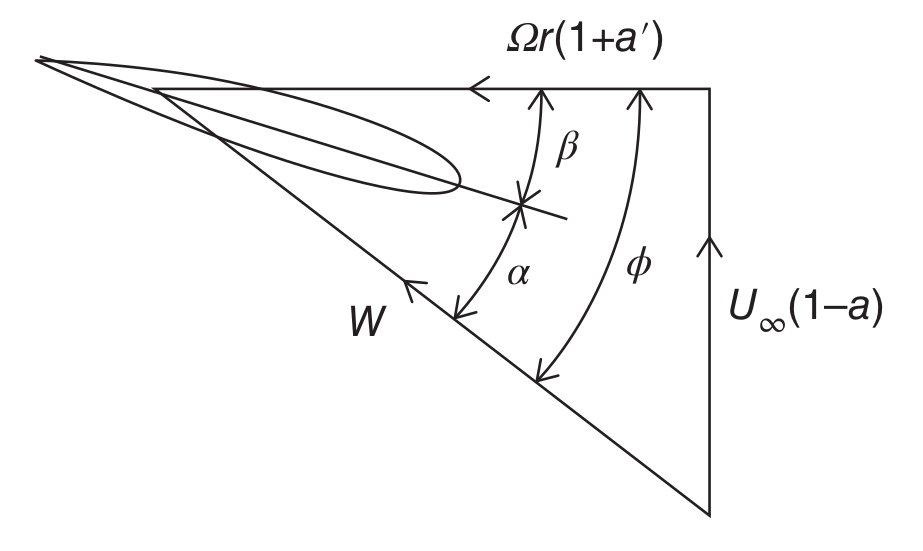
\includegraphics[width=0.9\linewidth]{./part1/figures/speed_triangle.png}
        \caption{Speed triangle}
    \end{subfigure}
    \begin{subfigure}[b]{0.5\textwidth}
        \centering
        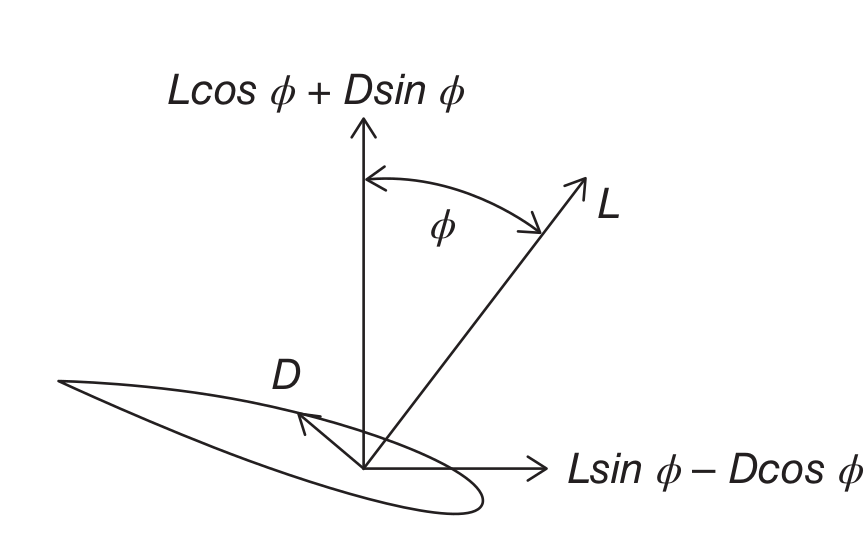
\includegraphics[width=0.9\linewidth]{./part1/figures/aerodyn_blade.png}
        \caption{Aerodynamic forces}
    \end{subfigure}
    \caption{Blade element forces. With the lift and drag forces $L$ and $D$, the flow angle $\phi$, the pitch angle $\beta$ and the angle of attack $\alpha$ (source: \citealt{burton_2021_wind_handbook}).}
    \label{fig:blade_theory}
\end{figure}
\textit{Blade element momentum theory} (BEMT) combines the results from blade element theory in \eq{eq:blade_element} with the results from momentum theory in \eq{eq:momentum_theory} to obtain the induction factors $a$ and $a'$. 
The resolution of this sytem of equations is often solved by iterative approaches (e.g., \citealt{dai_2011_BEMT}). 
Global axial thrust over the blade are then computed by integrating the elementary loads over all the elements. 
Note that various corrections are applied to the BEMT model, for example to take into account the non-homogeneous loss of momentum over the rotor disk. 
The BEMT also fails to model non-linear aerodynamic effects, occurring with sudden change of angle of attack. 
Such effects are sometimes called ``dynamic stall'' and are represented in DIEGO by the Beddoes-Leishman model (see \citealt{burton_2021_wind_handbook} for further details).  

%\elias{\paragraph{Aerodynamic damping?}}
%------------------------------------------------------------%
% See Petrovska p.51 


%============================================================%
\subsection{Hydrodynamics}
%============================================================%

Morison's equations are a widely-used semi-empirical model to assess the hydrodynamic forces on thin fixed structures such as offshore oil platforms and wind turbines. 
Considering a slender cylindrical structure of diameter $D$, a flow velocity $u(t)$, the drag and inertial coefficients $C_m$ and $C_D$, the axial force (parallel to the flow direction) is given by:   
\begin{equation}
    F\,=\,C_{m}\,\rho \,{\frac {\pi }{4}}D^{2}\,{\frac{\dd u}{\dd t}}\,+\,C_{d}\,{\frac 12}\,\rho \,D\,u\,|u|.
\end{equation}
Standard values for the drag and inertial coefficients are often considered \citep{dnv_2013_offshore_design}. 
DIEGO uses Morison’s equation together with first order potential solution to perform hydrodynamical simulations in the time domain.
An extended introduction to hydrodynamics of fixed slender structures, as well as large floating structures is given in the Chapter 1 from \citep{milano_thesis_2021}.  

To design floating structures, more complex wave loading modeling should be considered. 
For this purpose, \citet{ronge_2023_hydrodynamics_fowt} reviews nonlinear theories applied to the fluid-structure interactions of FOWT and compares them to CFD results. 


%============================================================%
\subsection{Control}
%============================================================%

To maximize their energy production under turbulent wind conditions, wind turbines rely on their control systems. 
This aspect of wind turbines is usually kept confidential by manufacturers, as it gives them a competitive advantage.  
Nevertheless, the general control mode of a wind turbine depends on the wind speed. 
Two main ranges of operation are usually defined: first between the cut-in and rated wind speed, second between the rated and cut-off wind speed. 
These characteristic wind speed values are given by the turbine manufacturer, for example a turbine may present a cut-in at $4~\si{m.s^{-1}}$, a rated at $13~\si{m.s^{-1}}$ and a cut-off at $25~\si{m.s^{-1}}$. 
Let us then recall the wind turbine power derived from the momentum theory: 
\begin{equation}
    P = \frac12 \rho \, A_d \, U_\infty^3 \, C_p(\lambda, \beta), 
    \label{eq:power_wt}
\end{equation}
with the power coefficient $C_p$, function of the pitch angle $\beta$ and the blade tip speed ratio $\lambda$, defined between the tangential speed on top of the blade and the wind speed: $\lambda = \frac{\Omega \, R}{U_\infty}$, for the rotation speed $\Omega$ and a rotor radius $R$. 

\paragraph{Below the rated wind speed.}
The goal of the control system is to extract as much power as available. 
A control strategy among the family of the \textit{maximum power point tracking} can be deployed \citep{abdullah_2012_control_review}.   
For example, the ``power signal feedback'' uses the electromagnetic torque to control the power. 
This method first computes the maxima of the extracted power as a function of the rotation speed (using \eq{eq:power_wt}), for different speed values. 
Then, for a measured wind rotation speed, the system can determine the reference maximal power. 
Considering this reference power, a controller (such as a proportional integral controller) intends to match the generated power with the reference by acting on the electromagnetic torque. 


\paragraph{Above the rated wind speed.}
The control system switches to a \textit{power limiting} mode by increasing the blades' pitch angles. 
By operating on the pitch, the rotation speed and the power produced are kept at their nominal values. 
This control is also often realized by a proportional integral system \citep{bossanyi_2003_pitch_control}. 

A more exhaustive description of wind turbines control systems is available in Chapter 8 from \citet{burton_2021_wind_handbook}. 
More recent strategies often consider the control at the farm scale. 
As explained earlier, the operation of one turbine affects the others via the effect of its wake. 
Moreover, since the wind energy production becomes important in the electric mix, its production might be constrained to respect the stability of the grid (e.g., quality of the utility frequency).  
The work of \citet{gionfra_2018_control} studied the optimal control of wind farms considering the effects of the wake and the grid restrictions. 

%============================================================%
\subsection{Structural dynamics}
%============================================================%

The structural elements of modern wind turbines, such as the tower and the blades, compose a dynamic system subject to important elastic deformations. 
Modeling an operating wind turbine therefore requires rigid body dynamics and nonlinear elastic deformations. 
All together, various approaches were developed to model the structural dynamics of wind turbines: modal analysis, multibody methods and finite element methods (FEM). 
At the stage of preliminary designs, modal approaches can be used to represent the dynamics under linear assumptions \citep{hegseth_2019_modal_FOWT}. 
Then, the tower's natural frequencies assessed by a modal analysis can be compared with the wind, waves, and the rotor's frequencies. 
As illustrated in \fig{fig:modal_analysis}, the structure's natural frequency (denoted by $f_0$) should not coincide with the main excitation frequencies to avoid critical dynamic resonance.
In the case of a wind turbine, the rotor imbalance creates a first dynamic load of frequency $f_{1P}$, while the blades passing in front of the tower generate a second excitation of frequency $f_{3P}$.  
The \textit{soft-stiff} design strategy places the structure's natural frequency between the two rotor frequencies (i.e., $f_{1P} < f_0 < f_{3P}$ as described in \fig{fig:modal_analysis}) and avoids main frequencies of the wind and waves. 
%\elias{Note that the wave spectrum is represented with a multimodal distribution}
\begin{figure}
    \centering
    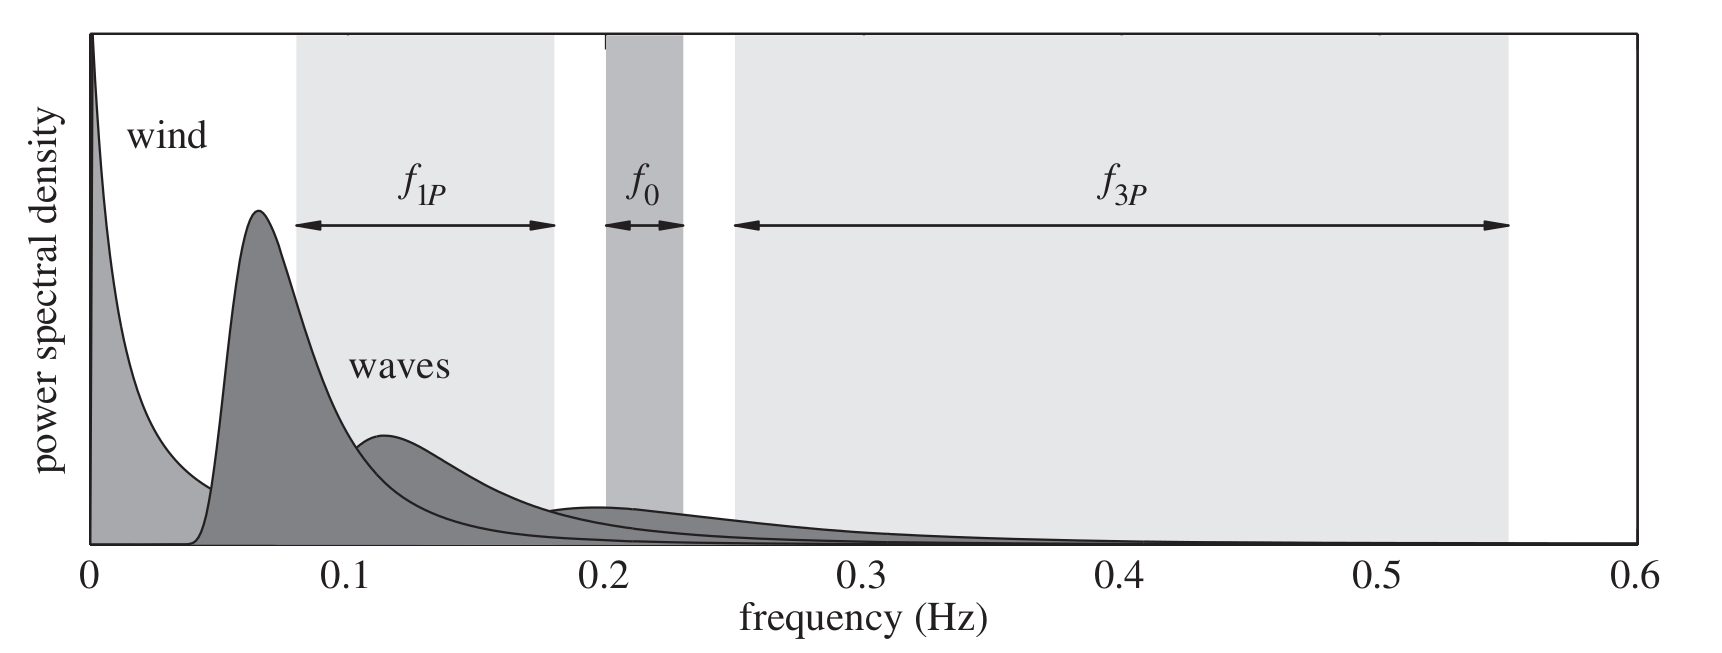
\includegraphics[width=0.75\textwidth]{./part1/figures/modal_analysis.png}
    \caption{Illustration of a soft-stiff design strategy, placing the structure's natural frequency $f_0$ away from the wind and wave power spectra, and the rotor excitation frequencies $f_{1P}$ and $f_{3P}$ (source: \citealt{kallehave_2015_modal}).}
    \label{fig:modal_analysis}
\end{figure}

However, modal analysis does not model transient loading phases and their corresponding non-linearities, which is crucial beyond early design. 
For a higher fidelity, simulations in the time domain using flexible multibody approaches are commonly used to describe the nonlinear dynamics \citep{holm_2009_multibody,alsolihat_2018_flexible_multibody}. 
DIEGO implements such an approach by combining rigid multibody dynamics with a deflection model based on Lagrangian equations \citep{milano_thesis_2021}. 
Note that for floating wind turbines modeling, a preliminary step of rigid body dynamics is added to define the coordinate system of the floater. 
\citet{otter_2022_owt_modeling_review} reviews the state-of-the-art of numerical and experimental modelling techniques for multi-physics OWT systems. 


%============================================================%
\subsection{Fatigue damage}\label{sec:235}
%============================================================%

Mechanical fatigue damage is an important phenomenon to consider when designing wind turbines. 
It refers to the progressive weakening of a material when subjected to cyclic or repeated loading, which may be significantly lower than the material's ultimate strength. 
Understanding the mechanisms behind mechanical fatigue damage is essential for designing durable and reliable structures. 
To quantify the fatigue damage on offshore wind turbine structures, standards \citep{dnv_fatigue_2016} recommend simulating the stresses in the time domain and identifying a series of stress cycles. 
Then, the \textit{stress-number of cycles curve} of a specific material (S-N curve) gives the number of cycles before failure at a given constant stress amplitude. 
As the stress cycles identified on the results of the OWT simulation are not constant, a linear aggregation method called \textit{Miner's rule} gathers the elementary damages over the stress time series studied. 


\paragraph{Stress cycles identification.}
%------------------------------------------------------------%
Offshore wind turbine simulators as DIEGO, deliver a time-dependent stress tensor. 
To ease the manipulation of this tensor, the equivalent Von Mises stress is computed, turning a multiaxial stress into an equivalent uniaxial stress. 
One can also consider a ``plane strain'' hypothesis on the Cauchy stress tensor $\underline{\underline{\sigma}}$, which is expressed as:
\begin{equation}
    \underline{\underline{\sigma}} = \begin{pmatrix}
                            \sigma_{11} & \sigma_{12} & 0\\
                            \sigma_{21} & \sigma_{22} & 0\\
                            0 & 0 & \sigma_{33}
                            \end{pmatrix}.
\end{equation}
This assumption simplifies the expression of the equivalent Von Mises stress: 
\begin{equation}
    \sigma _{\mathrm{VM}}=\sqrt{{\frac {1}{2}}\left[(\sigma _{11}-\sigma _{22})^{2}+(\sigma _{22}-\sigma _{33})^{2}+(\sigma _{33}-\sigma _{11})^{2}\right] + 3 \sigma _{12}^{2}}.
\end{equation}

Stress cycles can now be identified on the equivalent Von Mises stress time series. 
The usual method to identify fatigue stress cycles is called \textit{rainflow counting} \citep{dowling_1972}. 
In this approach, fatigue stress cycles are only defined by their amplitude (also called ``range'') and mean value, regardless of their chronology. 
Rainflow counting returns a list of stress ranges identified denoted by $s$ in the following. 


\paragraph{S-N curve.}
%------------------------------------------------------------%
The S-N curve is also called the ``W\"oler curve'' after the pioneer work of August W\"ohler, who demonstrated that fatigue damage was at the origin of railway accidents in the mid-19\textsuperscript{th} century \citep{schutz_1996_history_fatigue}. 
As a result of repeated fatigue experiments, this tool determines the number of similar stress cycles necessary to reach a fatigue ruin for a defined stress cycle amplitude. 
Its values depend on the material studied and on external conditions (i.e., in the offshore industry, the S-N curves distinguish the fatigue in the air vs. underwater). 

A well admitted simplification of the S-N curve is to consider it as log-linear\footnotemark on two segments:
\begin{equation}
\log(N_{\mathrm{c}}(s)) = \left\{
    \begin{array}{ll}
        \log(a_1) - m_1 \log(s), & \mbox{for}~ s \in [s_{\mathrm{min}}, s_{\mathrm{e}}] \\
        \log(a_2) - m_2 \log(s), & \mbox{for}~ s \in [s_{\mathrm{e}}, s_{\mathrm{max}}]
    \end{array}
\right.
\end{equation}
Where $N_{\mathrm{c}}$ is the predicted number of cycles to failure for stress range $s$, $m$ is the negative inverse slope of the S-N curve, 
$\log(a)$ is the intercept of log N-axis by the S-N curve, $s_{\mathrm{min}}$ is the minimal (resp. maximal) stress range identified by the rainflow counting, 
and $s_{\mathrm{e}}$ is the stress range axis of the intersection of the two log-lines formed by the S-N curve. 

\footnotetext{The logarithms related to the S-N curves in this document are logarithms in base 10.}

The expression of this curve in two linear segments arise from the concept of endurance limit of a material, $s_{\mathrm{e}}$, under which the effect of fatigue on a material should be considerably smaller. 
According to \cite{dnv_fatigue_2016}, the S-N curve is altered for welded tubular joints by taking into account the tube's thickness:
\begin{equation}
N_{\mathrm{c}}(s) = \left\{
    \begin{array}{ll}
        a_{1} \left(s (\frac{t}{t_{\mathrm{ref}}})^h\right) ^{-m_1}, & \mbox{for}~ s \in [s_{\mathrm{min}}, s_{\mathrm{e}}]\\
        a_{2} \left(s (\frac{t}{t_{\mathrm{ref}}})^h\right)^{-m_2}, & \mbox{for}~ s \in [s_{\mathrm{e}}, s_{\mathrm{max}}]
    \end{array}
\right.
\end{equation}
With $t_{\mathrm{ref}}$ the reference thickness (for tubular welded joints $t_{\mathrm{ref}}$ = 25 mm); $t$ the plate thickness, and $h$ the thickness exponent. 
The numerical values considered in the present work derive from the Section 2.4.6 of \citet{dnv_fatigue_2016}, reproduced in Table \ref*{tab:sn_table}. 

\begin{table*}[h]
    \centering
    \caption{S-N curve numerical values of welded tubular joints in different environmental conditions (source: \citealt{dnv_fatigue_2016})}
    \begin{tabular}{l|l|l|l|l|l}
     \hline
     \textit{Environment} & $m_1$ & $log(a_1)$ & $m_2$ & $log(a_2)$ & $h$\\
     \hline
     Air & $3.0$ & $12.48$ & $5.0$ & $16.13$ & $0.25$\\
     Seawater with cathodic protection & $3.0$ & $12.18$ & $5.0$ & $16.13$ & $0.25$\\ Seawater free corrosion & $3.0$ & $12.03$ & $3.0$ & $12.03$ & $0.25$\\ 
    \end{tabular}
    \label{tab:sn_table}
\end{table*}

\paragraph{Non-zero mean correction.}
%------------------------------------------------------------%
Most S-N curves are built over zero mean stress cycles, however, different empirical models were developed to consider different stress mean $s_m$ \citep{suresh_1998_fatigue_book}. 
The S-N curve becomes a three-dimensional envelope depending on the number of cycles $N_c$, the stress amplitude $s$, and the mean stress $s_m$. 
The ``Goodman line'' and the ``Gerber parabola'' are two models relating the stress amplitude $s$ to the mean stress $s_m$:  
\begin{align}
    \mathrm{Goodman} &:\quad \frac{s}{s_e} + \frac{s_m}{R_m} = 1\\
    \mathrm{Gerber} &:\quad \frac{s}{s_e} + \left(\frac{s_m}{R_m}\right)^2 = 1
\end{align}
Where the material's yield stress is denoted by $R_m$ and the endurance limit by $s_e$. 
The Haigh diagram represented in the \fig{fig:haigh_diagram} is a slice of the three-dimensional envelope for fixed values of fatigue endurance (i.e., number of cycles). 
By comparing the two models visually, the Goodman line is more conservative and is mostly used in the literature. 
Further discussion in the field of wind turbines was proposed in the early 2000s with a focus on the fatigue endurance of glass fiber materials \citep{sutherland_2000_fatigueWT}. 
In the present work, the non-zero correction presented above are not considered as the values of mean stress were found to be negligible compared to the yield stress of the steel material studied. 

\begin{figure}
    \centering
    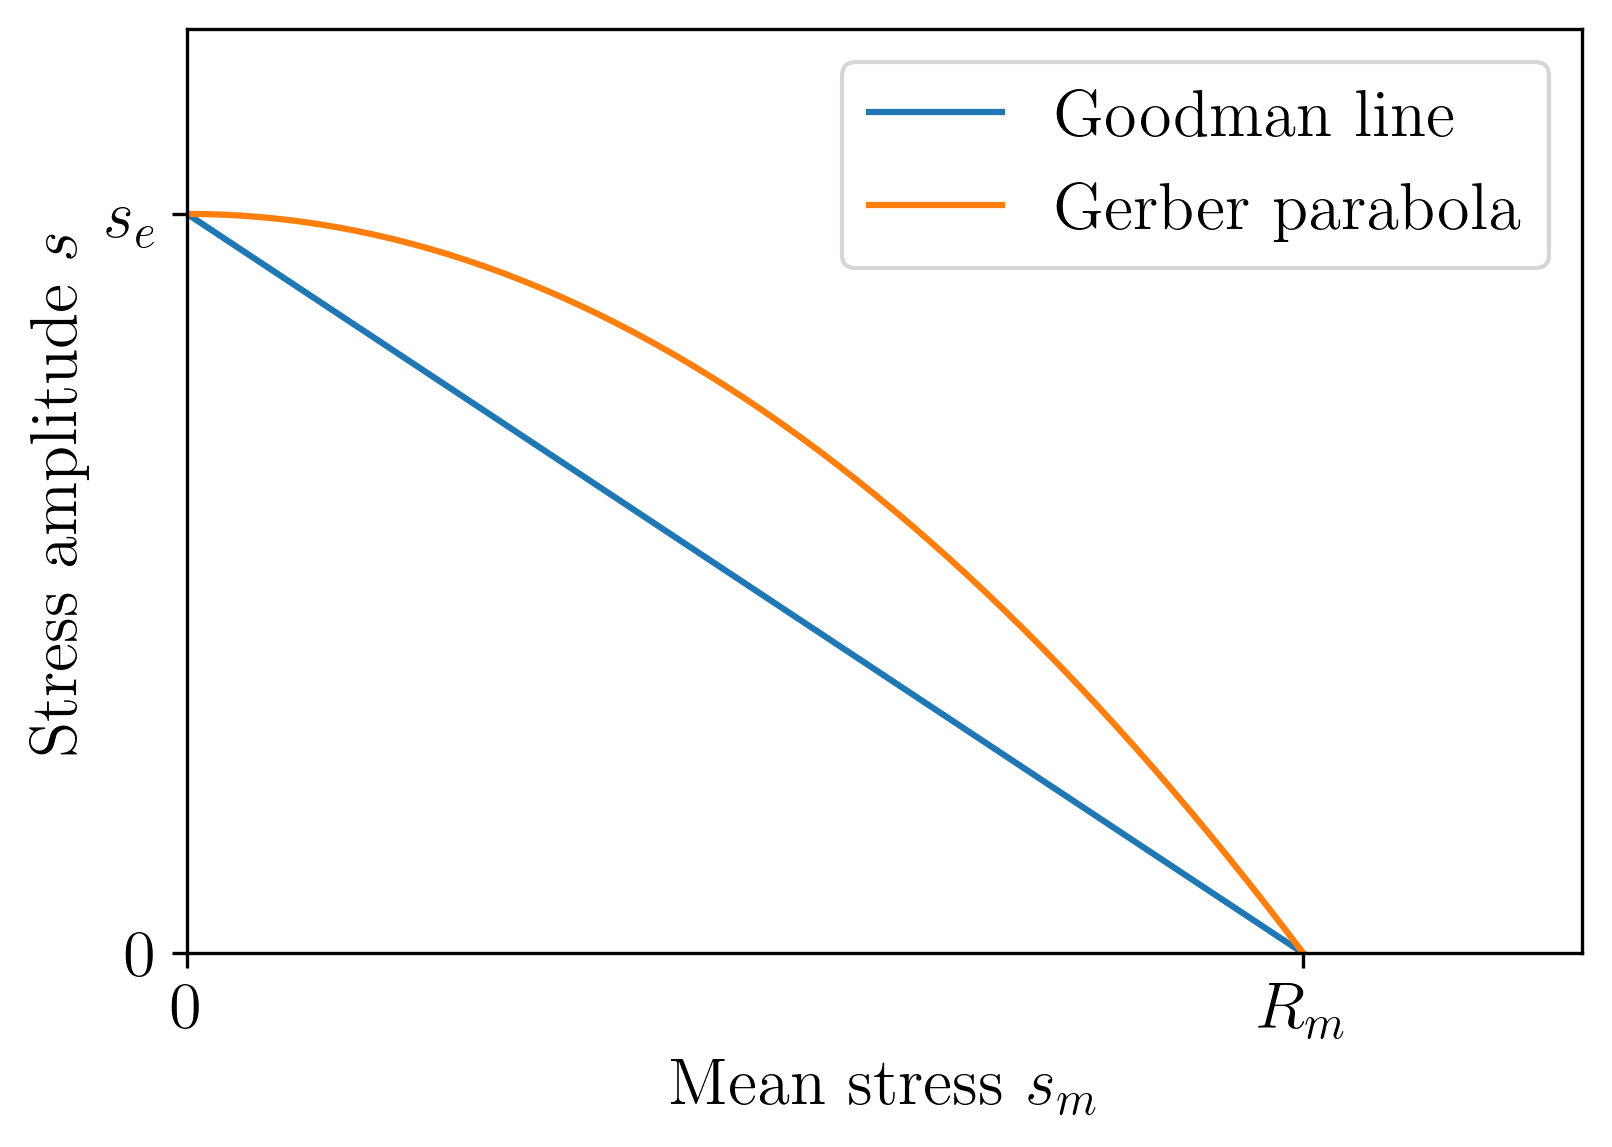
\includegraphics[width=0.5\textwidth]{../numerical_experiments/chapter2/figures/haigh_diagram.png}
    \caption{Illustration of the Haigh diagram representing the combination of stress mean and amplitude leading to the same fatigue endurance.}
    \label{fig:haigh_diagram}
\end{figure}



\paragraph{Cumulative damage theory.}
%------------------------------------------------------------%
A popular approach to assess the damage cumulated on a stress time series is to consider the fatigue contribution of each stress cycle according to the S-N curve. 
Palmgren-Miner's rule defines the \textit{cumulative damage} $d_c$ by summing the fatigue contributions of each stress cycle $k$, regardless of their order of appearance:
\begin{equation}
    d_c = \sum_{j=1}^{k} \frac{1}{N_{\mathrm{c}}\left(s^{(j)}\right)}.
    \label{eq:miner}
\end{equation}
In this theory, the material reaches fatigue ruin when the cumulative damage exceeds one.  
A common practice when using Palmgren-Miner's rule is to gather the stress cycles in a set of bins. 
This practice induces an integration error, which becomes significant as the number of bins is reduced. 
In the following, the cumulative damage is computed without binning, as defined in \eq{eq:miner}.


Spectral methods were also introduced to quantify fatigue damage in the late 80s. 
The main idea is to infer a PDF over the amplitudes of the stress cycles identified by rainflow counting, typically using a mixture of parametric distributions. 
From this PDF, one can derive the fatigue endurance and therefore a cumulated damage (see further details in the review of \citealt{dirlik_2021}). 
In the context of wind turbine fatigue assessment, spectral approaches showed to be unsuited in some cases (e.g., for blades' fatigue \citealt{ragan_2007_dirlik_vs_miner}).  
Overall, fatigue estimation in the time-domain does not represent important computational effort compared to the simulation of the wind turbine's physics. 

Nonlinear fatigue models were developed in the 90s \citep{fatemi_1998} to take into account the order in which the loading cycles were applied to the structure. 
For offshore wind turbine applications, the recent work of \citet{rocher_2020_nonlinear_fatigue} studied a probabilistic version of a nonlinear fatigue models. 
Unfortunately, this refined approach requires a larger computational effort and the calibration over experimental tests of various parameters \citep{freyssinet_2023_nonlinear_fatigue}.  


%============================================================%
%============================================================%
\section{Design and operation practices} \label{sec:owt_design}
%============================================================%
%============================================================%

The design and operation of offshore wind turbines is at the intersection of various engineering, environmental and social considerations. 
Regardless of the different bottom-fixed or floating technologies, OWTs are dynamically excited structures evolving in a harsh offshore environment.   
To operate such assets over up to 25 years of lifespan, multiple aspects should be assessed, from soil modeling, studies of environmental impact, grid integration, manufacturing quality, port logistics, to marine growth management, and maintenance. 
This section resumes the main types of OWT technologies, as well as the main design and operation practices.   

%============================================================%
\subsection{Types of technologies and preliminary design}
%============================================================%
The multiple OWTs technologies developed over the last two decades can be gathered into two groups: bottom-fixed or floating technologies. 
\fig{fig:FOWT_bottomfixed} and \ref{fig:FOWT_floating} respectively illustrates the different types of bottom-fixed or floating technologies. 
At this stage, the bottom-fixed solutions present more maturity while floating technologies are still transitioning from the phase of large demonstrators to industrial wind farms. 
In France, the current development of offshore wind energy lead to the construction of the two first industrial projects (both managed by EDF Renewables). 
On the coast of Saint-Nazaire, 80 bottom-fixed wind turbines were built on monopile foundations, altogether producing up to 480 MW. 
On the Mediterranean coast, the first French industrial floating project was recently installed 20 km offshore the coast of Marseille. 
This pilot project, called ``\textit{Provence grand large}'', is composed of three turbines operating on so called ``tension-leg platforms'', delivering 25 MW of nominal power.     

In order to lift water depth limitations associated with bottom fixed technologies (technical limit around 60 meters), floating pilot projects emerge across the world. 
However, the wind energy industry still tests different floating technologies in terms of cost efficiency and durability (as listed in \citealt{mackinnon_2022_FOWT_table}). 
An example of some farm projects with different types of technologies is described hereafter: 
\begin{itemize}
    \item \textbf{Semi-submersible}: a pilot project of three 10MW turbines called ``\textit{les éoliennes du Golfe du Lion}'' in the south of France relies on a semi-submersible technology developped by the company Principle Power \citep{cermelli_2018_windfloat}.   
    \item \textbf{Tension-leg}: a pilot project of three 8MW turbines called ``\textit{Provence grand large}'' exploits tension-leg platforms co-developped between the IFPEN national laboratory and the company SBM \citep{caille_2017_TPL_IFPEN}. 
    \item \textbf{Barge}: a pilot project of three 10MW turbines called ``EOLMED'' uses the floater developped by the company Ideol \citep{guignier_2016_ideol}. 
    \item \textbf{Spar}: the Norwegian oil and gas company Equinor chose the spar technology \citep{driscoll_2016_hywind} to equip its floating wind farm of 88MW, named ``Hywind Tampen''. 
\end{itemize}

\begin{figure}
    \begin{subfigure}[b]{0.48\textwidth}
        \centering
        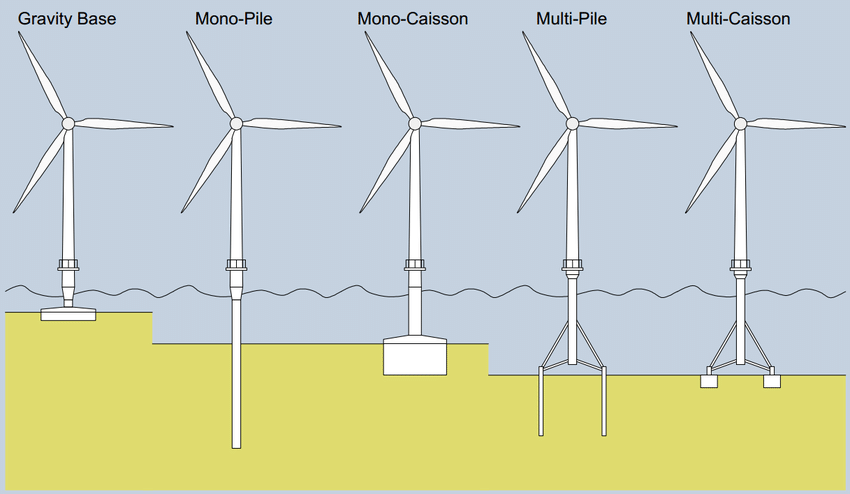
\includegraphics[width=\linewidth]{./part1/figures/bottom_fixed_techno.png}
        \caption{Bottom-fixed}
        \label{fig:FOWT_bottomfixed}
    \end{subfigure}
    \begin{subfigure}[b]{0.48\textwidth}
        \centering
        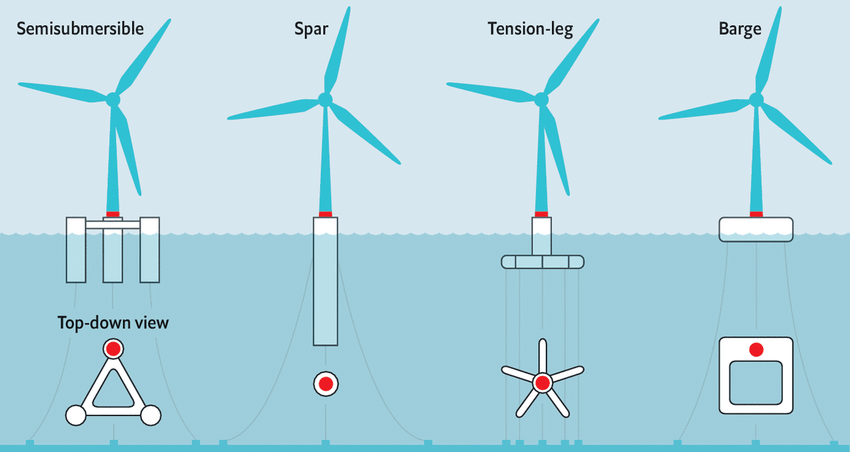
\includegraphics[width=\linewidth]{./part1/figures/Floating-wind-platform-categories.png}
        \caption{Floating}
        \label{fig:FOWT_floating}
    \end{subfigure}
    \caption{Main offshore wind turbine technologies (sources: \citealt{ahmed_2015_bottomfixed_image,mei_2021_FOWT_illustration}).}
\end{figure}



The turbines installed offshore over bottom-fixed foundations or floating structures present the same properties and components. 
As described in \fig{fig:owt_diagram}, the structure of a wind turbine is composed of blades made in composite materials, while the tower, the transition peace and foundation (e.g., monopile) are made out of steel. 
The steels used for the foundation and the tower are typical structural steels (i.e., steels with low carbon concentration such as the S355). 

Inside the nacelle, the gearbox adapts the rotation speed to suit the energy conversion system (i.e., generator). 
To improve the reliability of the components, manufacturers offer without gearboxes, called ``direct-drive''. 
This technology is relevant offshore, as the maintenance constraints are higher. 
However, the corresponding generators used in this situation operate at lower rotation speed. 
Adapting the generators significantly increase their weight and requires the use of larger permanent magnets increasing their price.   

The construction of an offshore wind farm requires several years of project planning, administrative procedures, consultation of the public opinion, and design. 
Internationals standards define the recommended practices and requirements related to the design and operation of OWTs. 
Among them, the IEC 61400 is subdivided in many parts, including the general one \citep{iec_2019} and other parts detailing specific topics.       
To validate the structural integrity of a wind turbine design, the standards recommend simulating the behavior of the OWT (using the methods described in Section \ref{sec:owt_modeling}) for many environmental conditions, called ``design load cases'' (DLC). 
As the environmental conditions depend on the site studied, the standards provide generic DLCs depending on a rough classification of the environmental conditions. 
Following the terminology in civil engineering, the structure is designed for ``fatigue limit states'' (FLS) and ``ultimate limit states'' (ULS) with respect to the environmental conditions. 
For fatigue, advanced sampling methods relying on environmental data measured on site will be introduced in Chapter 4. 
Beyond the main solicitations resulting from environmental loading, various aspects should be considered around offshore wind turbines. 

\begin{figure}
    \centering
    \begin{subfigure}[b]{0.3\textwidth}
        \centering
        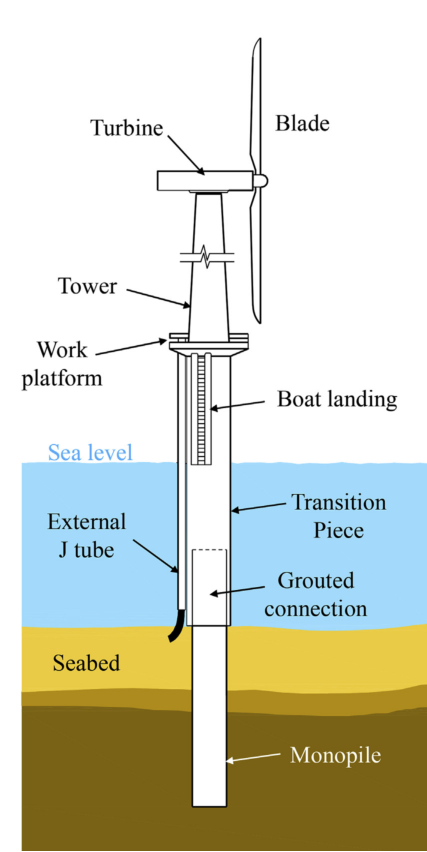
\includegraphics[width=0.7\linewidth]{./part1/figures/owt_diagram.pdf}
        \label{fig:struc_components}
        \caption{Monopile structure diagram}
    \end{subfigure}
    \begin{subfigure}[b]{0.48\textwidth}
        \centering
        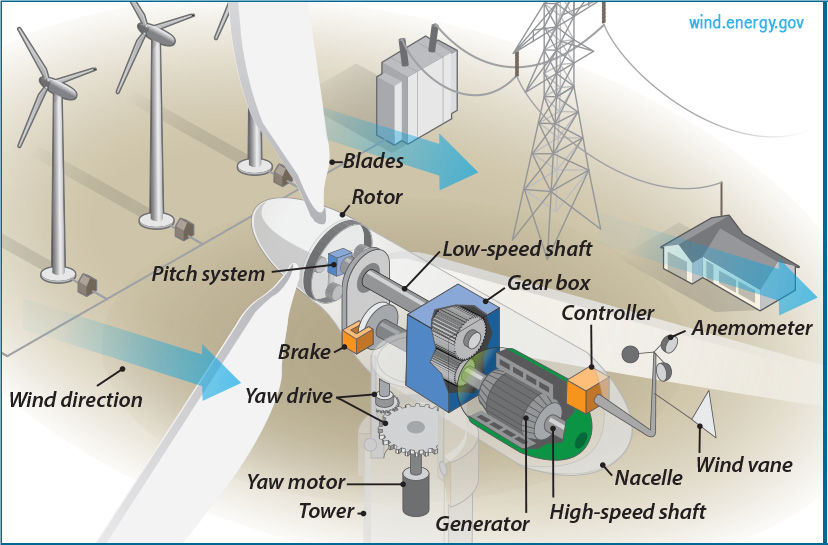
\includegraphics[width=\linewidth]{./part1/figures/nacelle_components.png}
        \caption{Major components in the nacelle}
        \label{fig:nacelle_components}
    \end{subfigure}
    \caption{Diagrams of an offshore wind turbine structure (source: \citep{chen_2018_owt_diagram}) and nacelle (source: US ODE).}
    \label{fig:owt_diagram}
\end{figure}

%============================================================%
\subsection{Further design considerations}
%============================================================%
The present section focuses on different topics to be addressed ahead of, or during the design and operation of offshore wind turbines.

\paragraph{Soil modeling.}
%------------------------------------------------------------%
The accurate geotechnical description of an offshore site plays an important role in the design and stability of bottom-fixed offshore wind turbines. 
The seabed soil properties are far from uniform in a wind farm, forcing the designer to adapt the foundations within a farm. 
Prior to the installation, geotechnical surveys and soil testing are conducted to assess parameters such as soil composition, density, strength, and seabed stability. 

To model the dynamic behavior of foundations, certification companies adapted their the methods from the oil \& gas industry to the offshore wind energy \citep{dnv_2018_soil}. 
For monopile foundations, the ``$p-y$'' method is often used to model soil-structure interactions. 
Assuming that these interactions are purely lateral, this method defines a set of non-linear lateral springs along the foundation's height.  
Together, the springs model the relation between the soil resistance ``$p$'' and the lateral displacement ``$y$''. 
Generally speaking, monopile foundations for OWT tend to be more rigid than for oil \& gas platforms, as the cyclic loading on wind turbines induces more fatigue (see the case-study presented in \citet{le_2014_geotech_casestudy}).  
However, various contributions in wind energy extended the use of $p-y$ curves to the case of multidirectional and irreversible displacements \citep{lovera_2019_thesis}. 
In summary, geotechnical considerations are essential for offshore wind turbine design, and the variability of soil properties within a wind farm necessitates a tailored approach to foundation design. 
Finally, the consideration of uncertainties in this field is still an open research topic \citep{reale_2021_OWT_soil_uncertainties}.

%\elias{Describe the modeling method in DIEGO called the ``apparent fixity'', and the defined soil stiffness matrix. See Petrovska p.52.}


\paragraph{Marine growth.}
%------------------------------------------------------------%
The bio-colonization of offshore structures and submarine cables is a significant concern in the maintenance and operation of OWTs. 
Elements exposed to the colonization of marine organisms, such as mussels, can cause several adverse effects. 
Firstly, the added weight increases the mass of the turbine and its foundation, potentially changing the dynamics of the systems and its structural integrity \citep{ameryoun_2019_marine_growth,schoefs_2022_reliability_marine_growth}. 
Secondly, marine growth changes the surface's roughness of the submerged components, which can create fluctuating hydrodynamic loads and vibrations \citep{marty_2021_cable_marine_growth}. 
To limit its impact on the reliability of OWTs, this phenomenon is addressed with regular preventive cleaning measures as part of the maintenance planning. 


\paragraph{Global scour.}
%------------------------------------------------------------%
The large-scale erosion of seabed sediment around bottom-fixed offshore wind turbine foundations, also called ``global scour'', poses different problems. 
The stability of the foundation is first reduced, potentially leading to tilting. 
Moreover, the load distributions changes, causing uneven stresses and increased fatigue. 
Finally, submarine cable exposure increases the risk of damage and electrical faults. 
As global scour is a critical element of the long-term OWT reliability, various mitigation measures are reviewed in \citet{fazeres_2021_scour}, including scour protection, and scour-robust foundation design.


\paragraph{Port logistics.}
%------------------------------------------------------------%
In the installation and maintenance of such large scale systems, port logistics plays an important role considering the international supply chain involved. 
The coordination, transportation and assembly of massive wind turbine components, foundations, and supporting infrastructure requires meticulous planning and execution. 
In accordance, the costs of handling operations and maintenance represent an important share of the \textit{levelized cost of energy} (LCOE) \citep{shields_2021_owt_lcoe}.  

In his review of OWT installation techniques, \citet{jiang_2021_owt_installation_review} describes the foundations' and components' installation processes depending on the OWT technology. 
Because of their large scale, most structural assembly (e.g., blades, or floater) are done on dedicated port docks, making the port choice critical.  
The assembled turbines are then transferred offshore with specialized vessels, such as installation jack-ups. 
Timing and synchronization are critical, as weather windows for handling operations can be limited.


\paragraph{Grid integration.}
%------------------------------------------------------------%
Unlike traditional centralized energy productions plants (i.e., nuclear and fossil), wind energy has considerable impact on the grid management. 
The intermittency of offshore wind generation is driven by variable wind conditions, which disrupts the electricity supply \citep{heier_2014_grid_integration}. 
Then, grid balancing becomes more complex as variable and distributed production sources are introduced.  
Wind turbine integration often require more flexibility from the grid, resulting in grid infrastructure upgrades (e.g., energy storage) and advanced grid management. 


\paragraph{Environmental impact and social acceptance.} 
%------------------------------------------------------------%
The fast development of offshore wind turbines in Europe raises questions regarding environmental and social impact. 
In their review, \citet{galparsoro_2022_owt_ecological_impact} showed that the installation and operation was shown to disrupt marine ecosystems.  
Further studies should be realized to better understand the reliance of the ecosystems to this change. 
This industry also affects other marine activities (e.g., fishing or tourism), and costal landscapes, which need to be discussed during the regional marine spacial planning. 
Finally, social acceptance of offshore wind projects varies across Europe, often split between local disturbances and the regional economic activity generated.  


\paragraph{Manufacturing quality.}
%------------------------------------------------------------%
The manufacturing of structural wind turbine components is subject to several uncertainties that can affect the overall quality and performance of OWTs. 
For example, the manufacturing process of composite blades can lead to inconsistencies in the final product. 
Imperfections in the composite material, like air pockets or delamination, can weaken the blades and reduce their lifespan. 
Additionally, variations in manufacturing processes can result in differences in blade weight, which impacts the turbine's performance. 
Regarding steel components, OWTs are mostly assembled by bolted and soldered joint. 
Inconsistent soldering, variations in material properties, and potential flaws in the joints can compromise the structural integrity of OWTs \citep{veers_2019_review}. 
These uncertainties in manufacturing quality can pose significant challenges in ensuring the reliability and longevity of the structures. 
Note that at the design phase, \textit{stress concentration factors} are defined by standards to take into account the local change in material properties created by soldering. 
Rigorous quality control, material testing, and manufacturing standards are essential to maintain the safety and efficiency of wind energy installations. 


\paragraph{Maintenance and end-of-life management.}
%------------------------------------------------------------%

To ensure the continued performance and availability of wind turbines, advanced maintenance planning is essential. 
Maintenance activities involve inspections, repairs, component replacements, and addressing issues as corrosion, or electrical faults. 
Preventive maintenance strategies (reviewed by \citet{ren_2021_owt_maintenance}) minimize the asset's unavailability and extends its lifespan. 

Once the wind farms reach their planned lifetime (typically between 20--25 years), the operator has the choice between decommissioning, ``repowering'', or ``revamping'' the assets. 
Usually, revamping implies an intermediate renovation of the WT. 
In most cases, the underperforming major components are replaced while the structural components are kept. 
Alternatively, repowering is a strategy reusing the foundations of a wind farm to install brand new furbines. 
This approach is often an opportunity to increase the scale and performances of the old turbines. 

As the first generation of wind farms currently reach their end-of-life, an important problematic raises from recycling large amounts of blades made out of composite materials. 
Different processes for recycling composite material are reviewed in \citet{jensen_2018_blade_recycling}, including mechanical, pyrolysis and chemical techniques. 
However, recycling composites is a complex and energy-consuming operation, that needs to be further studied. 
The recent lifecycle study of floating OWT in the Mediterranean region by \citet{pulselli_2022_FOWT_lifecycle} showed that effective maintenance and 
proper decommissioning planning are essential for ensuring cost-effective yet durable lifecycle management.  




%============================================================%
%============================================================%
\section{Uncertain inputs} \label{sec:owt_uncertainties}
%============================================================%
%============================================================%

Following the general diagram of uncertainty quantification in \fig{fig:UQ_methodo}, this section focuses on the definition of the uncertain inputs and their corresponding probabilistic model (step B). 
In our case, the generic term of ``inputs'' refers to the inputs to the wind turbine numerical model illustrated in \fig{fig:owt_chained_model}, which will be considered as random afterwards. 

The random variables studied in this work are split into two groups (assumed independent) which are respectively called \textit{environmental variables} and \textit{system variables}. 
First, the environmental variables are a collection of variables characterizing the long-term metocean conditions near a wind farm.
Even if the associated random vector presents a complex dependence structure, this source of variability is well-defined after the wind potential measurement campaigns. 

The second group of uncertain inputs is related to the wind turbine system. 
A wide range of uncertainties can be taken into account in such systems, such as material properties, manufacturing quality, soil conditions, control error, corrosion, marine growth, aerodynamic damping, etc.  
Among them, a restricted list of four variables are kept according to sensitivity analysis results from the literature and expert knowledge. 
%The present section defines the two groups of random variables, including a focus on the definition of probabilistic S-N curves. 


%============================================================%
\subsection{Environmental inputs}
%============================================================%

During the planning and operation of a wind farm project, the metocean conditions are studied using different sources of information. 
At the early stage, datasets generated by fine mesoscale numerical simulation can be used to assess the wind potential. 
This was typically the case during the call for tenders\footnote{\url{https://eolbretsud.debatpublic.fr/}} issued by the French government regarding the construction of two floating offshore wind farm in the south coast of Brittany (of respectively 250 and 500 MW of nominal power). 
Open-access environmental data of the sea-states in this reagion were available, as a result of mesoscale simulations \citep{raoult_2018_anemoc3} realized by EDF R\&D.    
In a second time, the local conditions are measured using a meteorological mast with wind speed cup anemometers at different heights and wave boys are generally installed in the vincity of the future farm. 
As a cheaper alternative to met masts, new measurement technologies such as floating LIDARs (standing for ``light detection and ranging'') were studied by \citet{gottschall_2017_floating_LIDAR}. 
Then, different adequation methods between the local measures and the data obtained by mesoscale simulations were reviewed in \citet{sempreviva_2008_wind_assessment_review}.  
Finally, after the installation of the turbines, the acquisition system (usually called SCADA, for ``supervisory control and data acquisition'') measures wind conditions with a sampling period of ten minutes. 

In the present work, two wind farms projects are partially studied: the Teesside wind farm, operating in the North Sea, and the south Brittany floating project, at the stage of tenders call. 
Table \ref{tab:envi_variables} summarizes the variables considered as random hereafter. 
The inference of such data will be discussed in Chapter \ref{chpt:3} of this manuscript. 
Note that the environmental data resulting from the SCADA system of the Teesside wind farm is confidential, and will be represented as anonymized data in the following. 

\begin{table}[h!]
    \centering
    \begin{tabular}{ l l l}
        \hline
        {\it Name} & {\it Notation} & {\it Description}\\
        \hline
        Mean wind speed & $U$ & 10-min. average horizontal at 10m\\
        Turbulence & $\sigma_s $ & 10-min.  standard deviation \\
        Wind direction & $\theta_{wind} $ & Wind directions\\
        Significant wave height & $H_s $  & Significant wave height per hour\\
        Peak wave period & $T_p $ & Peak 1-hour spectral wave period \\
        Wave direction & $\theta_{wave} $ & Wave directions\\
        %Mean shear & $\alpha$ & Normal & 10-min mean shear exponent \\
        %Air density & $\delta$ & - & -\\
        \hline
    \end{tabular}
    \caption{Marginal distributions of the environmental random variables}
    \label{tab:envi_variables}
\end{table}

%============================================================%
\subsection{System inputs}
%============================================================%
As mentioned earlier, multiple parameters in a wind turbine system can be considered as uncertain. 
Our study focuses on the effects of uncertainties on the fatigue damage over the structure. 
Therefore, the literature review of the sensitivity analysis on offshore wind turbine fatigue helped us narrow down a few system variables. 
\citet{petrovska_2022} explored the sensitivity analysis of many variables on the fatigue of a wind turbine in Teesside. 
Even if the use of the Morris method is questionable, the results allowed to screen out some variables. 
For example, the uncertainties related to the corrosion, the wind shear exponent, or the nacelle mass showed a limited impact on the fatigue.     
By crossing the conclusions of various research with the expert knowledge among partners from the HIPERWIND European project, the system variables considered uncertain in the following are summarized in Table \ref{tab:sys_variables}. 
Each of them is assumed independent, with a marginal probabilistic model arising from the literature. 


\begin{table}[h!]
    \centering
    \begin{tabular}{ l l l l}
        \hline
        {\it Name} & {\it Notation} & {\it Marginal model} & {\it Description}\\
        \hline
        Soil coefficient & $S$ & Normal ($\mu=1., \sigma=0.3$) & Applied to the soil stiffness matrix\\
        Yaw misalignment & $\theta_{\mathrm{m}}$ & Normal ($\mu=0., \sigma=0.3$) & Error in wind alignment\\
        SN curve coefficient & $a$ & Log-normal ($\mu=1, \sigma=0.3$) & See \cite{guede_2007}\\
        Critical damage & $D_{\mathrm{cr}}$ & Log-normal ($\mu=1, \sigma=0.3$) & See \cite{drexler_musculus_2021}\\\hline
    \end{tabular}
    \caption{Marginal distributions of the system random variables}
    \label{tab:sys_variables}
\end{table}



\subsection{Probabilistic fatigue assessment}
%------------------------------------------------------------%
The definition of a fatigue endurance model has a main impact on fatigue damage assessment. 
However, the S-N curves usually describing the endurance of a material are built on repeated laboratory experiments. 
Even if the need for random S-N curves has long been expressed in the field of fatigue experiments \citep{lieurade_1982_essais_fatigue}, their probabilistic description was better formalized in \citep{guede_2007,sudret_2013_fatigue}. 

The models proposed in \citet{guede_2007} are based on the experimental procedure used to build the S-N curves. 
For identical steel specimens, a cyclic loading with fixed amplitude is repeated until fatigue ruin. 
Because of variations in the material's microstructure, the fatigue endurance for the same cyclic solicitation is random. 
This variation is commonly assumed to follow a log-normal distribution in the literature. 
A probabilistic model of the S-N curve naturally comes: 
\begin{subequations}
    \begin{align}
        \log(N_c(s, \omega)) &= \log(a) - m \log(s) + \log(\varepsilon(\omega))\\
        \Rightarrow N_c(s, \omega) &= a \, s^{-m} \, \varepsilon(\omega),
    \end{align}
\end{subequations}
where $\log(\varepsilon(\omega)) \sim \mathcal{N}(0, \sigma_{N_c}=0.2)$ is assumed when no measurement is available (according to Appendix F.5 from \citealt{dnv_fatigue_2016}). 

This uncertainty can be injected in the Miner-Palmgren rule defined in \eq{eq:miner}: 
\begin{equation}
    d_c(\omega) = \sum_{j=1}^k \frac{1}{N_c(s^{(j)}, \omega)}
            = \sum_{j=1}^k \frac{1}{a \, \left(s^{(j)}\right)^{-m} \, \varepsilon(\omega)}
            = \frac{1}{\varepsilon(\omega)} \sum_{j=1}^k \frac{1}{a \, \left(s^{(j)}\right)^{-m}}
\end{equation}
Then, this uncertainty can be assessed as a pure post-processing of fatigue damage results computed with a single deterministic S-N curve. 

In wind energy standards, S-N curves for design are actually a conservative envelope of the measured fatigue endurance. 
Annex F.7 from \citet{dnv_fatigue_2016} describes how to define a design S-N curve from fatigue measures. 
Assuming that the fatigue endurance follows a Gaussian distribution (on logarithmic scale), the design S-N curve $N_c^{\mathrm{design}}(s)$ is the curve at two standard deviations $\sigma_{N_c}$ below the median curve. 

Using the design S-N curve given in Section 2.4.6 \citet{dnv_fatigue_2016} and the normality assumption, one can reconstruct the median S-N curve by taking: 
\begin{equation}
    q_{50\%}[\log(N_c(s, \omega))]= \log(N_c^{\mathrm{design}}(s)) + 2 \, \sigma_{N_c}. 
\end{equation}

\fig{fig:probabilistic_SN} illustrates the design curve defined by DNV for tubular joints (in Section 2.4.6) and the reconstructed probabilistic model according to the previous assumptions. 

\begin{figure}
    \centering
    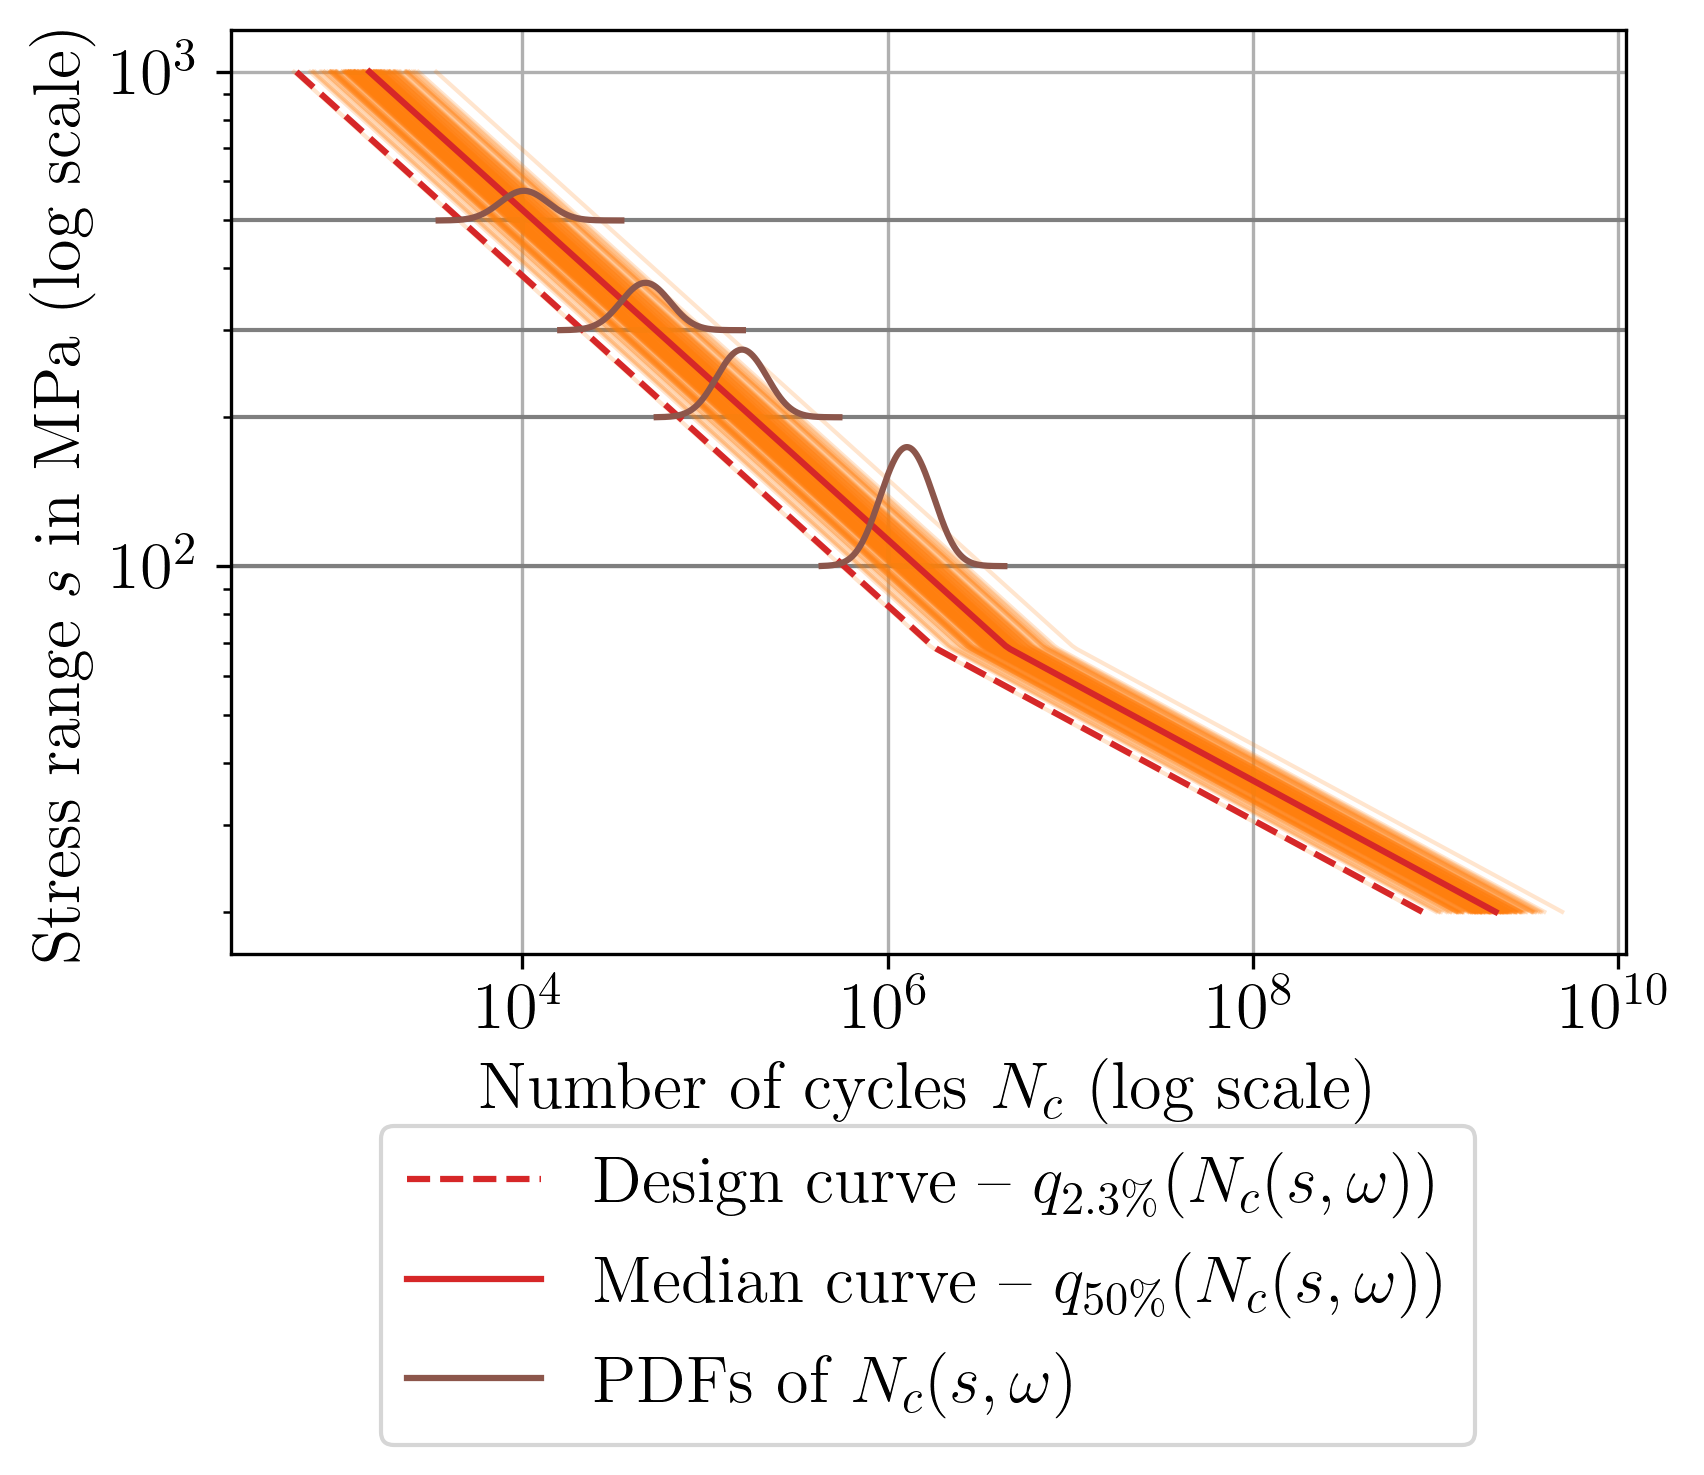
\includegraphics[width=0.6\textwidth]{../numerical_experiments/chapter2/figures/probabilistic_fatigue.png}
    \caption{Illustration of a probabilistic S-N curve according to the model defined in \citet{guede_2007}.}
    \label{fig:probabilistic_SN}
\end{figure}


%============================================================%
%============================================================%
\section{Conclusion}
%============================================================%
%============================================================%

This chapter proposed an overview on offshore wind turbine modeling and design. 
It introduced concepts related to the description and simulation of metocean conditions. 
The impact of the wake on the performance and on unsymmetrical fatigue loading was also explained.  
Then, the different theories considered in OWT modeling were introduced such as aerodynamics, hydrodynamics, structural dynamics and control. 
A variety of softwares implementations exist for this purpose, but a special attention was brought on DIEGO a numerical model developed by EDF R\&D. 
As a perspective, uncertainty quantification could benefit from the different fidelities proposed to model OWT systems presenting very nonlinear transient phases. 

To understand the design of OWTs, the most common technologies of bottom-fixed and floating turbines were presented. 
Then, a focus on a few critical topics to be considered during design and exploitation was proposed. 
In the light of the previous elements, the variables considered as random in this work were listed with a particular focus on probabilistic fatigue.   

This growing industry faces various challenges, for example related to the important use of primary commodities, the cohabitation of offshore dynamic structures with an ecosystem, composite materials recycling, etc. 
Uncertainty quantification is a tool to understanding some of these problematics, however, many uncertainties are hard to characterize and quantify. 
For example, manufacturing quality issues were revealed by Siemens Gamesa\footnotemark regarding wrinkles on the surface of some blades. 


\footnotetext{L. Pitel and R.Millard. (August 7 2023). Siemens Energy warns of €4.5bn loss from ailing wind turbine division. \textit{Finacial Times}. \url{https://www.ft.com/content/df8947cd-4bab-46ff-804e-b28de4b5a0f0}}




\setlength\epigraphwidth{.37\textwidth}
\epigraphhead[550]{
    \epigraph{\textit{Le doute est un état mental désagréable, mais la certitude est ridicule.}}{\textsc{Voltaire}}
}
\part{Contributions to uncertainty quantification and propagation}
%!TEX root = ../thesis.tex
%*******************************************************************************
%*********************************** Third Chapter *****************************
%*******************************************************************************
\cleardoublepage
\chapter{Kernel-based uncertainty quantification}
\label{chpt:3}
%*******************************************************************************
\hfill
\localtableofcontents
\newpage


\begin{tcolorbox}[colback=gray!5!white, colframe=gray!5!white, coltitle=gray!70!white, coltext=gray!60!white, title=\textbf{Parts of this chapter are adapted from the following references:}]
    A. Lovera, E. Fekhari, B. Jézéquel, M. Dupoiron, M. Guiton and E. Ardillon (2023). ``Quantifying and clustering the wake-induced perturbations within a wind farm for load analysis". In: \textit{Journal of Physics: Conference Series (WAKE 2023)}.\\

    E. Vanem, E. Fekhari, N. Dimitrov, M. Kelly, A. Cousin and M. Guiton (2023). ``A joint probability distribution model for multivariate wind and wave conditions''. In: \textit{Proceedings of the ASME 2023 42th International Conference on Ocean, Offshore and Arctic Engineering (OMAE 2023)}.
\end{tcolorbox}

%============================================================%
%============================================================%
\section{Introduction}
%============================================================%
%============================================================%
The main sources of solicitation in offshore design reside in the metocean conditions. 
To accurately verify a structural design against the joint wind and wave conditions, these random excitations must be carefully modelled. 
Offshore structures are usually certified against ultimate limit states (related to the occurrence of extreme metocean conditions) and fatigue limit states (related the average fatigue over the metocean conditions). 
In this context, the probabilistic framework is typically used to model the joint distribution of random variables describing the metocean conditions (listed in Section~\ref{sec:owt_uncertainties}). 

Note that a given probabilistic model might describe well the central behavior of the environmental distribution but not its tail behavior (and vice-versa).   
Extreme value theory develops specific methods to model the far tails of distributions \citep{beirlant_2006_extreme_values}. 
Modeling the tails is not the priority in the present work since the focus is on mean fatigue estimation.   

The environmental random variables studied present different particularities. 
First, an offshore wind turbine project leads to the collection of an important amount of metocean data (possibly merged with data from mesoscale simulations). 
Second, their dependence structure is complex, making the probabilistic modeling more complicated. 

This chapter explores different aspects of the environmental conditions' uncertainty quantification. 
The theory of some nonparametric copulas is introduced before their use in metocean conditions inference. 
A semiparametric approach is applied on the South Brittany data, mixing parametric modeling of the marginals with nonparametric modeling of the copula. 
To visually analyze multivariate distributions, the \textit{copulogram} is a new tool that decomposes the marginal effects and the dependence structure of a joint distribution. 

At the scale of a wind farm, each turbine perceives different metocean conditions as the wake of other turbines creates wind perturbations. 
To study this perturbation, an engineering wake model (see Section~\ref{sec:222}) was used to obtain one perturbed environmental distribution per turbine. 
This work applies a kernel-based discrepancy (the maximum mean discrepancy) to compare wake induced perturbations. 
In a second time, this discrepancy is used to gather wind turbines perceiving similar perturbations. 
This clustering can be used to perform uncertainty propagation at the farm scale by considering a few turbines with are representative of a cluster. 


%============================================================%
%============================================================%
\section{Dependence modeling with nonparametric copula}\label{sec:nonparametric_copula}
%============================================================%
%============================================================%

In uncertainty quantification, the lack of knowledge can lead to rough assumptions regarding the dependence modeling. 
However, an accurate representation of the uncertain inputs is of prime importance. 
For example, the work of \citet{torre_2019_copula_reliability} demonstrates the influence of the dependence model on the estimation of rare event probabilities by studying the same problem with different copula models. 

When inferring a probabilistic model over a multivariate dataset, one can decompose the problem into the fit of a set of marginals and the fit of a copula (see the Sklar Theorem \ref{thm:sklar}). 
In the case of metocean conditions, the fit of the marginals is not problematic considering the amounts of data available. 
However, the complex dependence structure appears to be more challenging. 
Different strategies to model the dependence for multivariate distributions are shortly summarized hereafter: 
\begin{itemize}
    \item \textbf{Vine copulas} (also known as pair copula) decompose the joint distribution as a product of conditioned bivariate copulas organized in a tree-like structure called a vine. 
    This approach proved to be very efficient, but it requires the definition of the vine and the bivariate parametric copulas \citep{joe2011dependence}. 
    \item \textbf{Conditional modeling} defines the joint distribution as a product of univariate conditional distributions. 
    In practice, the parameter of a marginal are defined as a function of other marginals (see e.g., \citealt{vanem_fekhari_2023}). 
    %This approach is widely used to model metocean conditions, but its implementation is not always straightforward. 
    \item \textbf{Multivariate KDE} is another way to capture the dependence together with marginal effects. As the dimension and the size of the dataset increase, this method become less tractable \citep{wand_jones_1994_kde}.  
    \item \textbf{Nonparametric copulas} are methods uniformly approximating an empirical copula without any assumption on a dependence structure. They will be further described and used for metocean conditions inference in the present chapter.    
\end{itemize}

\begin{remark}
    The strategy referred as ``conditional modeling'' can in fact be expressed as a copula \citep{vanem_2016} for continuous variables. For example, in the bivariate case of a continuous random vector $\bX = (X_1, X_2)$ with PDF $f_\bX(\bx)$, CDF $F_\bX(\bx)$ and density copula $c$: 
    \begin{subequations}
        \begin{align}
            f_\bX(\bx) &= f_{X_1}(x_1) \, f_{X_2|X_1}(x_2|x_1) = f_{X_1}(x_1) \, f_{X_2}(x_2) \, c\left(F_{X_1}(x_1), F_{X_2}(x_2)\right)\\
            \Leftrightarrow & c\left(F_{X_1}(x_1), F_{X_2}(x_2)\right) = \frac{f_{X_1}(x_1) \, f_{X_2|X_1}(x_2|x_1)}{f_{X_1}(x_1) \, f_{X_2}(x_2)}
        \end{align}  
    \end{subequations}
\end{remark}

The notions related to the copula theory are further introduced in the monographs of \citet{nelsen_2006_copulas,joe_2014,durante_2015_copula} while the key properties are introduced hereafter.


%============================================================%
\subsection{Preliminary definitions and properties}\label{sec:copula_prelims}
%============================================================%
%Soit X = (X 1 , . . . , X n ) T un vecteur aléatoire de dimension n défini sur l’espace
%n
%probabilisé (Ω, A, P) et soit x = (x 1 , . . . , x n ) T ∈ R une réalisation de X. La définition
%de copule est facilitée en introduisant les notions de face inférieure et bord supérieur
%de I n :
Let us consider a random vector $\bX \in \iD_{\bx}\subseteq\R^d$ defined on a probability space $(\Omega, \iA, \P)$. 
Its probability distribution $\P_\bX$ can be represented by a CDF $F_\bX$ and PDF $f_\bX$. 
The functional definition of a \textit{d-dimensional copula} (or simply ``d-copula'') is a density function $C:[0, 1]^d \mapsto [0, 1]$ whose marginals are uniformly distributed on $[0, 1]$.
\begin{theorem}[Copula]
    A function $C:[0, 1]^d \mapsto [0, 1]$ is a d-copula if, and only if, it presents the following properties:
    \begin{itemize}
        \item The function $C$ is ``grounded'' (also called ``anchored''): \\$C(u_1, \dots, u_d) = 0$ if $u_j=0, \, \forall j\in\{1, \dots, d\}$;
        \item The marginals of $C$ are uniform, then: $C(1, \dots, u_j, \dots, 1) = u_j,  \, \forall j\in\{1, \dots, d\}$;
        \item The function $C$ is ``d-increasing'', meaning that for any hyperrectangle $A \subset [0, 1]^d$, the corresponding volume induced by $C$ is positive (see \cite{durante_2015_copula} p.7). 
    \end{itemize}
    \label{thm:copula}
\end{theorem}

A copula is bounded by two functions according to the Fréchet-Hoeffding bounds. 
\begin{theorem}[Fréchet-Hoeffding bounds]
    If a function $C:[0, 1]^d \mapsto [0, 1]$ is a d-copula, then it respects the following bounds for all $\bu \in [0, 1]^d$: 
    \begin{equation}
        W(\bu) = \max (1 - d + u_1 + \dots + u_d, \, 0) \, \leq C(\bu) \, \leq \, M(\bu) = \min(u_1,\dots ,u_d).
    \end{equation} 
    Where the upper bound $M$ is still a copula while the lower bound $W$ is only one for $d=2$.
\end{theorem}

The rank transform plays an essential role to understand copulas. 
Considering a continuous random vector $\bX \in \iD_{\bx}$ and the sample $\bX_n = \left\{\bx^{(1)}, \dots, \bx^{(n)}\right\} \sim \bX$, its \textit{ranks} $\bR_n = \left\{\br^{(1)}, \dots, \br^{(n)}\right\} \in \N^{n}$ correspond to the indexes of its order statistics: 
\begin{equation}
    r^{(i)}_j = n \, \what{F}_{X_j}(x_j^{(i)}) = \sum_{l=1}^n \1_{\left\{x^{(l)}_j \leq x^{(i)}_j\right\}}, \quad \forall j \in \{1, \dots d\}, i \in \{1, \dots n\},
    \label{eq:ranks}  
\end{equation}
where $\what{F}_{X_j}$ stands for the marginal empirical CDF associated to the random variable $X_j$.


\begin{theorem}[Rank-invariance]
    Considering a random vector $\bX=(X_1, \dots, X_d)$, a set of mappings $\{r_j (\cdot)\}_{j=1}^d$, and the image random vector $\bR=(r_j \circ X_1, \dots, r_d \circ X_d)$. 
    If the mappings are strictly increasing (which is the case for the rank transform introduced in \eq{eq:ranks}), then, the copula associated to $\bR$ is invariant by transformation: $C_\bX = C_\bR$. 
    A proof is presented in \citet{durante_2015_copula} p. 57.
\end{theorem}

Transforming in the ranks generally reduces the effect of outliers and ensures more robust estimates. 
The invariance by rank transform of copulas allows the estimation of different \textit{dependence measures} in the ranked space. 


\paragraph{Spearman's rho.} Is a well-known dependence measure, also called the ``Spearman's rank correlation coefficient'', which is defined for two random variables $X_i, X_j$ as: 
\begin{equation}
    \rho^{\mathrm{S}}(X_i, X_j) = \frac{\cov(r_i(X_i), r_j(X_j))}{\sigma_{r_i(X_i)} \, \sigma_{r_j(X_j)}},
\end{equation}
an equivalent definition exists, using the copula $C$ between the joint distribution of $X_i$ and $X_j$ and the independent copula $\Pi(u_i, u_j) = u_i \, u_j$: 
\begin{equation}
    \rho^{\mathrm{S}}(X_i, X_j) = 12 \int_{[0, 1]^2} C(u_i, u_j) \, \dd u_i \dd u_j - 3 = 12 \int_{[0, 1]^2} (C(u_i, u_j) - \Pi(u_i, u_j)) \, \dd u_i \dd u_j. 
\end{equation}

\paragraph{Kendall's tau.} Also referred to as the ``Kendall's rank correlation coefficient'', is defined for a pair of random variables $(X_i, X_j)$ and their respective independent copies $(X_i', X_j')$ as: 
\begin{equation}
    \tau(X_i, X_j) = \P\left((X_i - X_i')(X_j - X_j') > 0 \right) - \P\left((X_i - X_i')(X_j - X_j') < 0 \right),
\end{equation}
and can also be defined using the copula $C$ between the joint distribution of the two random variables: 
\begin{equation}
    \tau(X_i, X_j) = 4 \int_{[0, 1]^2} C(u_i, u_j) \, \dd C(u_i, u_j) - 1 = 1 - 4 \int_{[0, 1]^2} \frac{\partial C(u_i, u_j)}{\partial u_i} \frac{\partial C(u_i, u_j)}{\partial u_j} \, \dd u_i \dd u_j 
\end{equation}
These dependence measures fully rely on the copula and are both bounded between -1 and 1. 
Further properties and estimators of Spearman's rho and Kendall's tau are presented in \citet{durante_2015_copula} Section 2.4. 


\paragraph{Upper/lower tail dependence.} Considering the random vector $\bX = (X_i, X_j)$ and the copula $C$ underlying their joint distribution. 
The \textit{upper/lower tail dependence} coefficients are defined as: 
\begin{subequations}
    \begin{align}
        \lambda_U(X_i, X_j) &= \lim_{\substack{u \rightarrow 1 \\ u<1}} \, \P\left(X_i > F_{X_i}^{-1}(u) | X_j > F_{X_j}^{-1}(u)\right) =       \lim_{\substack{u \rightarrow 1 \\ u<1}} \left(2 - \frac{1 - C(u, u)}{1 - u}\right)\\
        \lambda_L(X_i, X_j) &= \lim_{\substack{u \rightarrow 0 \\ u>0}} \, \P\left(X_i \leq F_{X_i}^{-1}(u) | X_j \leq F_{X_j}^{-1}(u)\right) = \lim_{\substack{u \rightarrow 0 \\ u>0}} \left(\frac{C(u, u)}{1 - u}\right) 
    \end{align}
\end{subequations}
\cite{joe_2014} further discusses asymptotic limit and outlines the particular case of the bivariate Gaussian copula, for which the tail dependence measures are null, $\lambda_U = \lambda_L = 0$.
Note that Kendall's tau and the tail dependence coefficients both have their associated plots, allowing to compare the dependence of two distributions \elias{add ref}.

%============================================================%
\subsection{Empirical and checkerboard copula}
%============================================================%

The \textit{empirical copula} was introduced by \citet{deheuvels_1979_empirical_copula}, as an estimator of the copula $C$ associated with the random vector $\bX$. 
Since the normalized ranks are a creasing mapping that present uniform marginals by construction, they are a natural empirical representation of the density copula. 
Considering a sample $\bX_n = \left\{\bx^{(1)}, \dots, \bx^{(n)}\right\} \sim \bX$ with the respective ranks $\bR_n = \left\{\br^{(1)}, \dots, \br^{(n)}\right\}$, a definition of the empirical copula is: 
\begin{equation}
    C_n(u_1, \dots, u_d) = \frac1n \sum_{i=1}^{n} \prod_{j=1}^{d} \1 \left\{ \frac{r_j^{(i)}}{n} \leq u_j \right\}, \quad  \bu = (u_1, \dots, u_d) \in [0, 1]^d
    \label{eq:empirical_copula}
\end{equation}
Even if this function converges uniformly towards the copula $C$ (according to the Glivenko-Cantelli theorem), it does not fulfill the conditions to be a copula (see e.g., \citealt{gonzalez_2021_checkerboard_copula}). 

In this context, different methods may be applied to smooth the empirical copula into a genuine copula. 
This problem can be perceived as a functional approximation of the underlying copula $C$, which is unique for continuous variables (according to Sklar's Theorem \ref{thm:sklar}). 
Let us consider a discretization of the unit hypercube as a grid: 
\begin{equation}
    G=\left\{\frac{0}{m_1}, \dots, \frac{m_1}{m_1}\right\} \times \dots \times \left\{\frac{0}{m_d}, \dots, \frac{m_d}{m_d}\right\}, \quad \bm = (m_1, \dots, m_d) \in \N^d. 
\end{equation}

The \textit{checkerboard copula} is a simple approximation of the empirical copula using the discretization $G$. 
This method is comparable to a multivariate histogram of the empirical density copula $c_n$ (see the formal multivariate definition proposed by \citealt{cottin_2014_bernstein}).
In the particular case for which $m_j=m, \, \forall j \in \{1, \dots, d\}$, the checkerboard copula is called the ``rook'' copula, and expressed by \citet{segers_2017} as: 
\begin{equation}
    C_n^{\#m}(u_1, \dots, u_d) = \frac1n \sum_{i=1}^{n} \prod_{j=1}^{d} \min\left(\max(n\, u_j - r_j^{(i)} +1, \, 0), \, 1\right).
\end{equation}

This empirical copula has a low complexity (see \citealt{rose_2015}) and efficient results for large samples \citep{gonzalez_2021_checkerboard_copula}, however, its variance is comparable to the empirical copula for small-sized samples \citep{segers_2017}. 
It is proven to be a genuine copula and its asymptotic behavior was studied by various authors such as \citet{li_1998_checkerboard,genest_2017_asymptotic_checkerboard}. 
In the following, an approximation of the empirical copula with Bernstein polynomials is presented. 



%============================================================%
\subsection{Empirical Bernstein and Beta copula}
%============================================================%

A few elements on Bernstein polynomials and their corresponding approximation is reminded before introducing the empirical Bernstein copula.

\subsubsection{Bernstein polynomials and approximation}
%------------------------------------------------------------%
Let us first define the \textit{Bernstein basis polynomial} of order $m \in \N$ as: 
\begin{equation}
    b_{m, t}(u)= \binom{m}{t}u^t(1-u)^{m-t}, \quad t \in \{0, \dots, m\}.
\end{equation}
These polynomials present various interesting properties, such as their nonnegativity over $[0, 1]$, being bounded by one, and offering a partition of unity on $[0, 1]$ \citep{lasserre_2023_bernstein}: 
\begin{equation}
    1 = \sum_{t=0}^{n} b_{m, t}(u)(x), \quad \forall x\in\R, \quad \forall n \in \N.
\end{equation} 

Bernstein's polynomials allow us to uniformly approximate any continuous and real-valued function defined on a compact set $f: [0, 1]^d \mapsto \R$ (as they were used to demonstrate the Weierstrass approximation theorem). 
In the multivariate case, the \textit{Bernstein approximation} of the function $f$ can be written on a grid over the unit hypercube $G=\left\{\frac{0}{m_1}, \dots, \frac{m_1}{m_1}\right\} \times \dots \times \left\{\frac{0}{m_d}, \dots, \frac{m_d}{m_d}\right\}, \bm = (m_1, \dots, m_d) \in \N^d$, as: 
\begin{equation}
    B_{\bm}(f)(\bu) = \sum_{t_1=0}^{m_1} \dots \sum_{t_d=0}^{m_d} f\left(\frac{t_1}{m_1}, \dots, \frac{t_d}{m_d}\right) \prod_{j=1}^d b_{m_j, t_j}(u_j) \, , \quad  \bu = (u_1, \dots, u_d) \in [0, 1]^d.
    \label{eq:bernstein_approx}
\end{equation}
The Bernstein polynomials approximate $f$ such that $\lim_{m\to\infty} B_{m}(f) = f$ uniformly on $\left[0,1\right]$. 


\subsubsection{Bernstein polynomials for copula approximation}
%------------------------------------------------------------%
Copulas are continuous and bounded functions defined on a compact set (the unit hypercube). 
Therefore, they are good candidates to be approximated by Bernstein polynomials. 
The Bernstein approximation applied on an empirical copula $C_n$ was introduced as \emph{empirical Bernstein copula} (EBC) by \cite{sancetta_satchell_2004} for applications in economics and risk management: 
\begin{equation}
    B_{\bm}(C_n)(\bu) = \sum_{t_1=0}^{m_1} \dots \sum_{t_d=0}^{m_d} C_n\left(\frac{t_1}{m_1}, \dots, \frac{t_d}{m_d}\right) \prod_{j=1}^d b_{m_j, t_j}(u_j) \, , \quad  \bu = (u_1, \dots, u_d) \in [0, 1]^d.
    \label{eq:ebc}
\end{equation}
In this expression, the evaluations of the empirical copula on the vertices of the grid are smoothed by the product of Bernstein polynomials. 
A respective approximation of the copula density can be directly expressed by deriving the previous formula. 
The EBC delivers a genuine copula, if and only if all the polynomial degrees $\{m_j\}_{j=1}^d$ are divisors of $n$ (see \citealt{segers_2017}, Proposition 2.5). 

In the particular case of regular grids, $\{m_j=m\}_{j=1}^d$, the EBC can be expressed as a mixture of beta distributions \citep{segers_2017}. 
Let us consider an $n$-sized rank sample, $\bR=(\br_1, \dots, \br_d) \in \N^{n}$, and the degree $m$ taken as divisor of $n$. 
Note that the r\textsuperscript{th} order statistic of an $n$-sized sample following a uniform $[0, 1]$ is distributed according to the beta distribution $\mathcal{B}(r, n-r+1)$. 
Considering these hypotheses, the EBC can be written as: 
\begin{equation}
    B_{m}(C_n)(\bu) = \frac 1n \sum_{i=1}^n \prod_{j=1}^{d} F_{m, r_j^{(i)}} \, , \quad  \bu = (u_1, \dots, u_d) \in [0, 1]^d, 
\end{equation}
where $F_{m, r}$ is the CDF of the beta distribution $\mathcal{B}(r, m-r+1)$ (also called the ``regularized incomplete beta function''): 
\begin{equation}
    F_{m, r} = \sum_{t=r}^{m} \binom{m}{t}u^t(1-u)^{m-t}, \quad u \in [0, 1], \quad r \in \{1, \dots, m\}. 
\end{equation}

Overall, the EBC is a very versatile tool which able to approximate complex dependence patterns. 
Moreover, Monte Carlo sampling on an EBC is straightforward and licit since it is a genuine copula. 
As a drawback, the estimation accuracy of this nonparametric method heavily relies on the polynomial order tuning.   


\subsubsection{Asymptotic behavior of the empirical Bernstein copula}
%------------------------------------------------------------%
In practice, the choice of polynomial degree for an EBC leads to a challenging bias-variance tradeoff. 
For example, the particular case of $\{m = n\}$, introduced as the \textit{empirical Beta copula} by \cite{segers_2017}, tends to reduce the bias while increasing the variance. 
In this paper, the beta copula presents interesting results compared to the Bernstein or the checkerboard copula for small sample sizes (i.e., $n<100$). 
Theoretically, the tuning of the degree was first optimized to minimize an ``Asymptotic Mean Integrated Squared Error'' (AMISE) of $B_{\bm}(C_n)$: 
\begin{equation}
    \mathrm{AMISE}(B_{\bm}(C_n)) = \E\!\left[ \lVert B_{\bm}(C_n) - C \rVert^2_2 \right] \!=\! \E\!\left[\!\int_{\R^d}\! \left(B_{\bm}(C_n)(\bu) \!-\! C(\bu) \dd \bu \right)^2 \!\right]\!\!.
    \label{eq:aimse}
\end{equation}
The seminal work of \citet{sancetta_satchell_2004} proves in Theorem 3 that: 
\begin{itemize}
    \item $B_{\bm}(C_n)(\bu) \rightarrow C(\bu)$ for any $u_j \in \left]0, 1\right[$ if $\frac{m^{d/2}}{n} \rightarrow 0$, when $m, n \rightarrow \infty$.
    \item The optimal polynomial order in terms of AMISE is\footnotemark: $m \lesssim m_{\mathrm{AIMSE}} = n^{2/(d+4)}, \forall u_j \in \left]0, 1\right[$.    
\end{itemize}
\footnotetext{The sign $\lesssim$ stands for ``less than or approximately''.}
To illustrate the previous theorem, \fig{fig:hmise} represents the evolution of the $m_{\mathrm{AMISE}}$ for different dimensions and sample sizes (adapted from \citealt{lasserre_2022}). 
In medium dimension, the values of $m_{\mathrm{IMSE}}$ tend towards one, which is equivalent to the independent copula. 
Therefore, high-dimensional problems should rather be divided into a product of smaller problems on which the EBC is tractable.

\begin{figure}
    \centering
    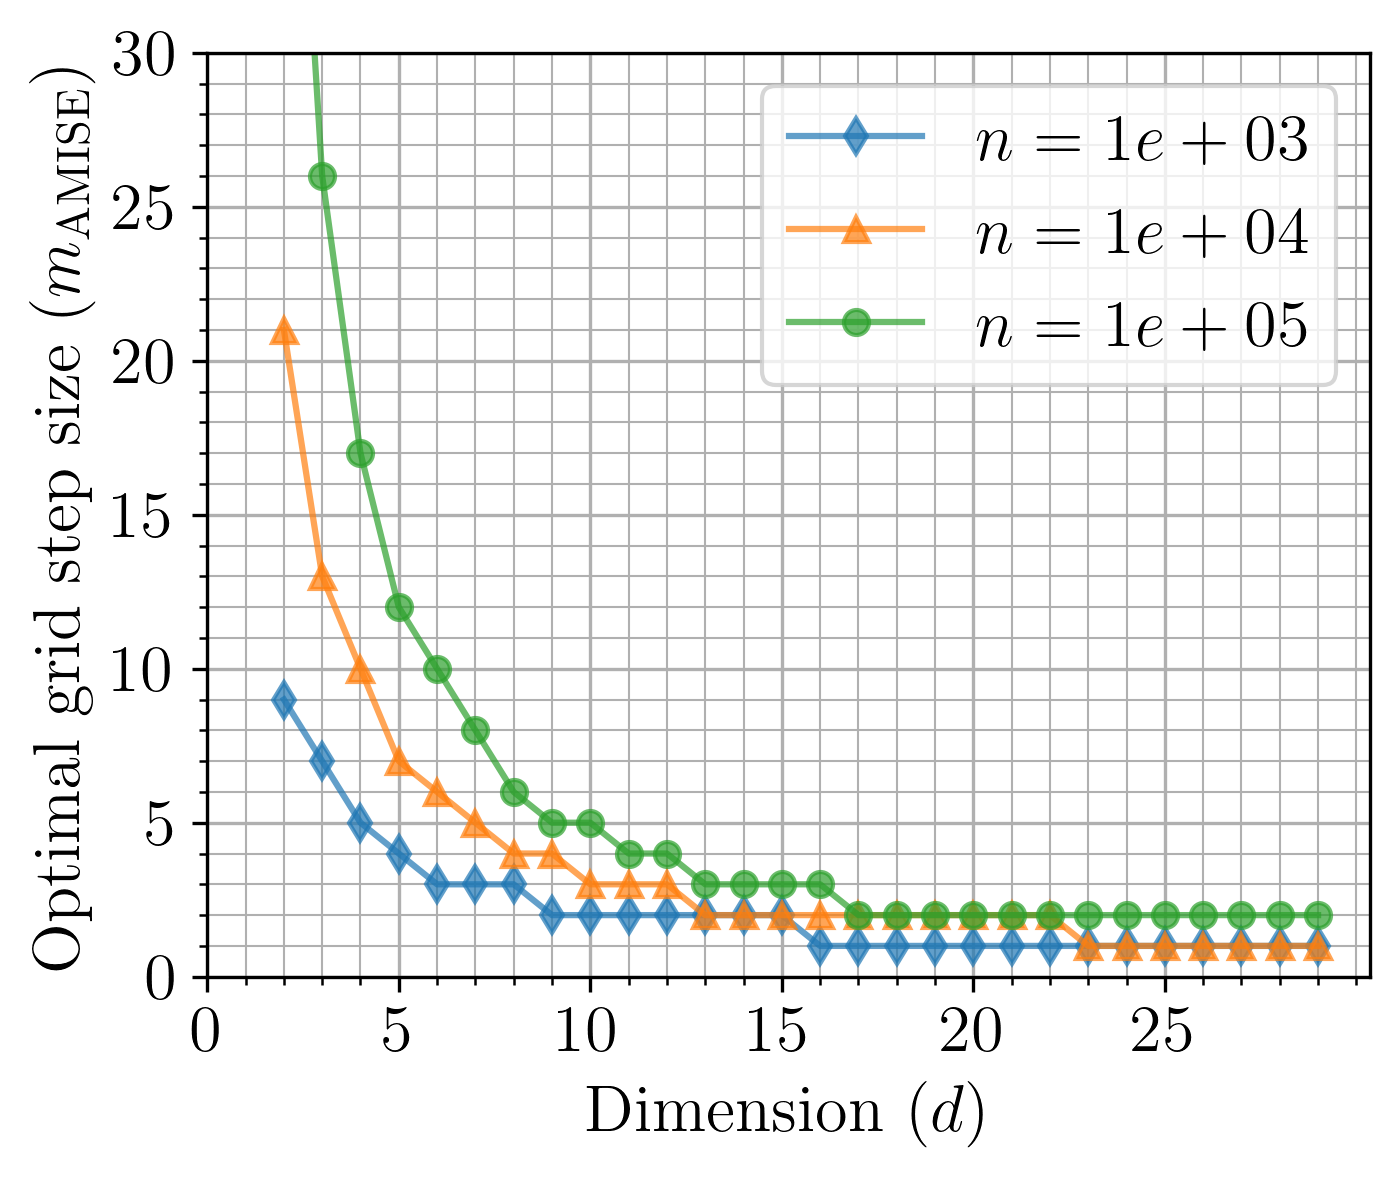
\includegraphics[width=0.5\linewidth]{../numerical_experiments/chapter3/figures/hAMISE.png}
    \caption{Evolution of $m_{\mathrm{IMSE}}$ for different dimensions and sample sizes.}
    \label{fig:hmise}
\end{figure}

The polynomial order for EBC estimation is still a bottleneck which was studied over the years by different authors (see e.g., \citealt{janssen_2012_ebc,bouezmarni_2013_EBC_convergence,rose_2015,segers_2017}).  
Meanwhile, other nonparametric approaches such as the ``penalized Bernstein'' and the ``penalized B-spline'' estimators were compared to the EBC and vine copulas in a benchmark realized by \citet{nagler_2017}. 
The results showed that the most performant methods vary depending on the problem studied (for different dimension, sample sizes, strength of dependence). 
Regarding tail dependence modeling, nonparametric approaches are generally limited, but recent contributions introduced Bootstrap procedures to better this aspect \citep{kiriliouk_2021_resampling}.


\subsubsection{Illustrative example on a Clayton copula}
%------------------------------------------------------------%
Let us consider a bivariate Clayton copula $C$ with parameter $\theta=2.5$ (see \citealt{nelsen_2006_copulas})
A Monte Carlo sample with size $n=10$ is generated on it, which is then used to build an empirical copula $C_n$ as defined in \eq{eq:empirical_copula}. 
\fig{fig:ebc_illustration} (a) illustrates the empirical copula corresponding to the sample, with the shade of grey matching the CDF values. 
Then, the Bernstein approximation of the empirical copula (i.e., the EBC)  is represented in \fig{fig:ebc_illustration} (b), (c), (d) according to the \eq{eq:ebc}. 
The three versions of the EBC correspond to different polynomial orders, assuming that $(m_1=m_2)$. 

As the order increases, the bias between the EBC and the copula $C$ tends to be reduced. 
Note that the second EBC in \fig{fig:ebc_illustration} (c) where $(m_1=m_2=n)$ is equivalent to the Beta copula. 
Moreover, increasing the order beyond the sample size definitely overfits of the copula. 

%\elias{possible alternative: 2D plots in two rows. Row 1: empirical copula/EBCn=5/EBCn=10. Row 2: empirical density copula/EBCn=5/EBCn=10.}

\begin{figure}
    \begin{subfigure}[b]{0.49\textwidth}
        \centering
        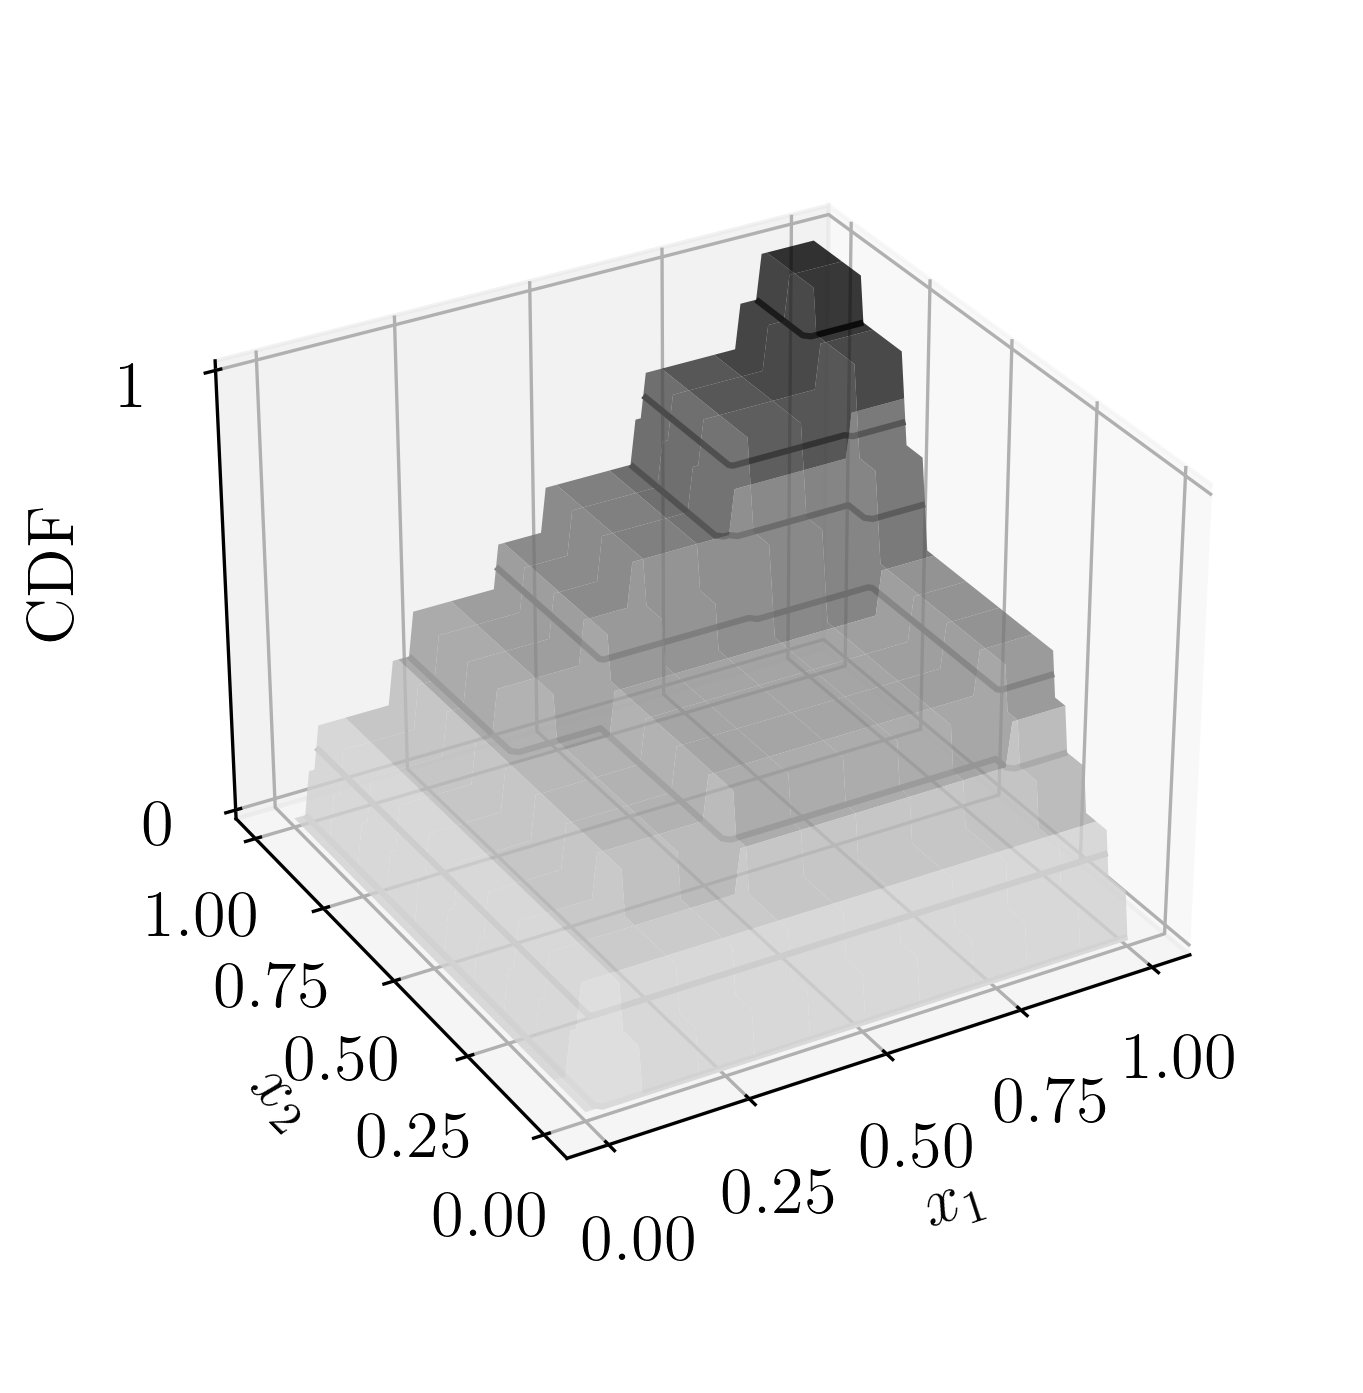
\includegraphics[width=\linewidth]{../numerical_experiments/chapter3/figures/empirical_copula.png}
        \caption{Empirical copula $C_n$ with ($n=10$).}
    \end{subfigure}
    \begin{subfigure}[b]{0.49\textwidth}
        \centering
        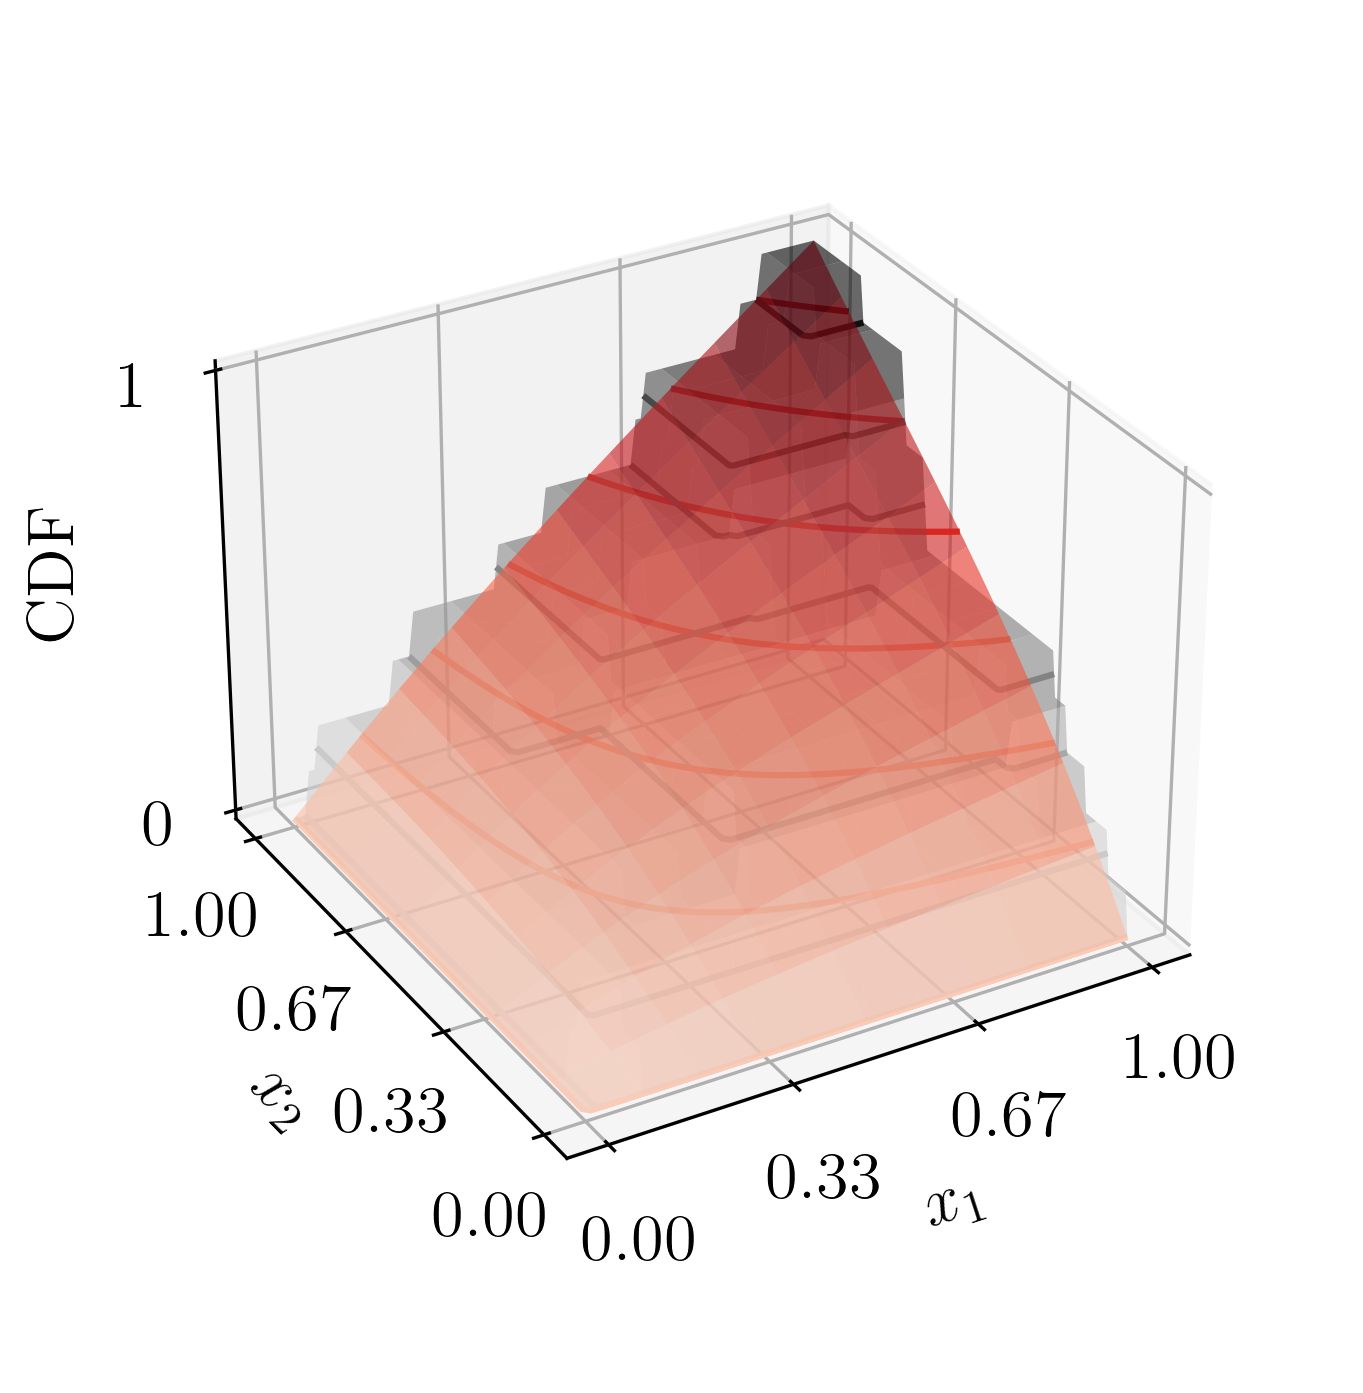
\includegraphics[width=\linewidth]{../numerical_experiments/chapter3/figures/ebc_m3.png}
        \caption{$B_{\bm}(C_n)$ with $(m_1=m_2=3)$.}
    \end{subfigure}
    \\
    \begin{subfigure}[b]{0.49\textwidth}
        \centering
        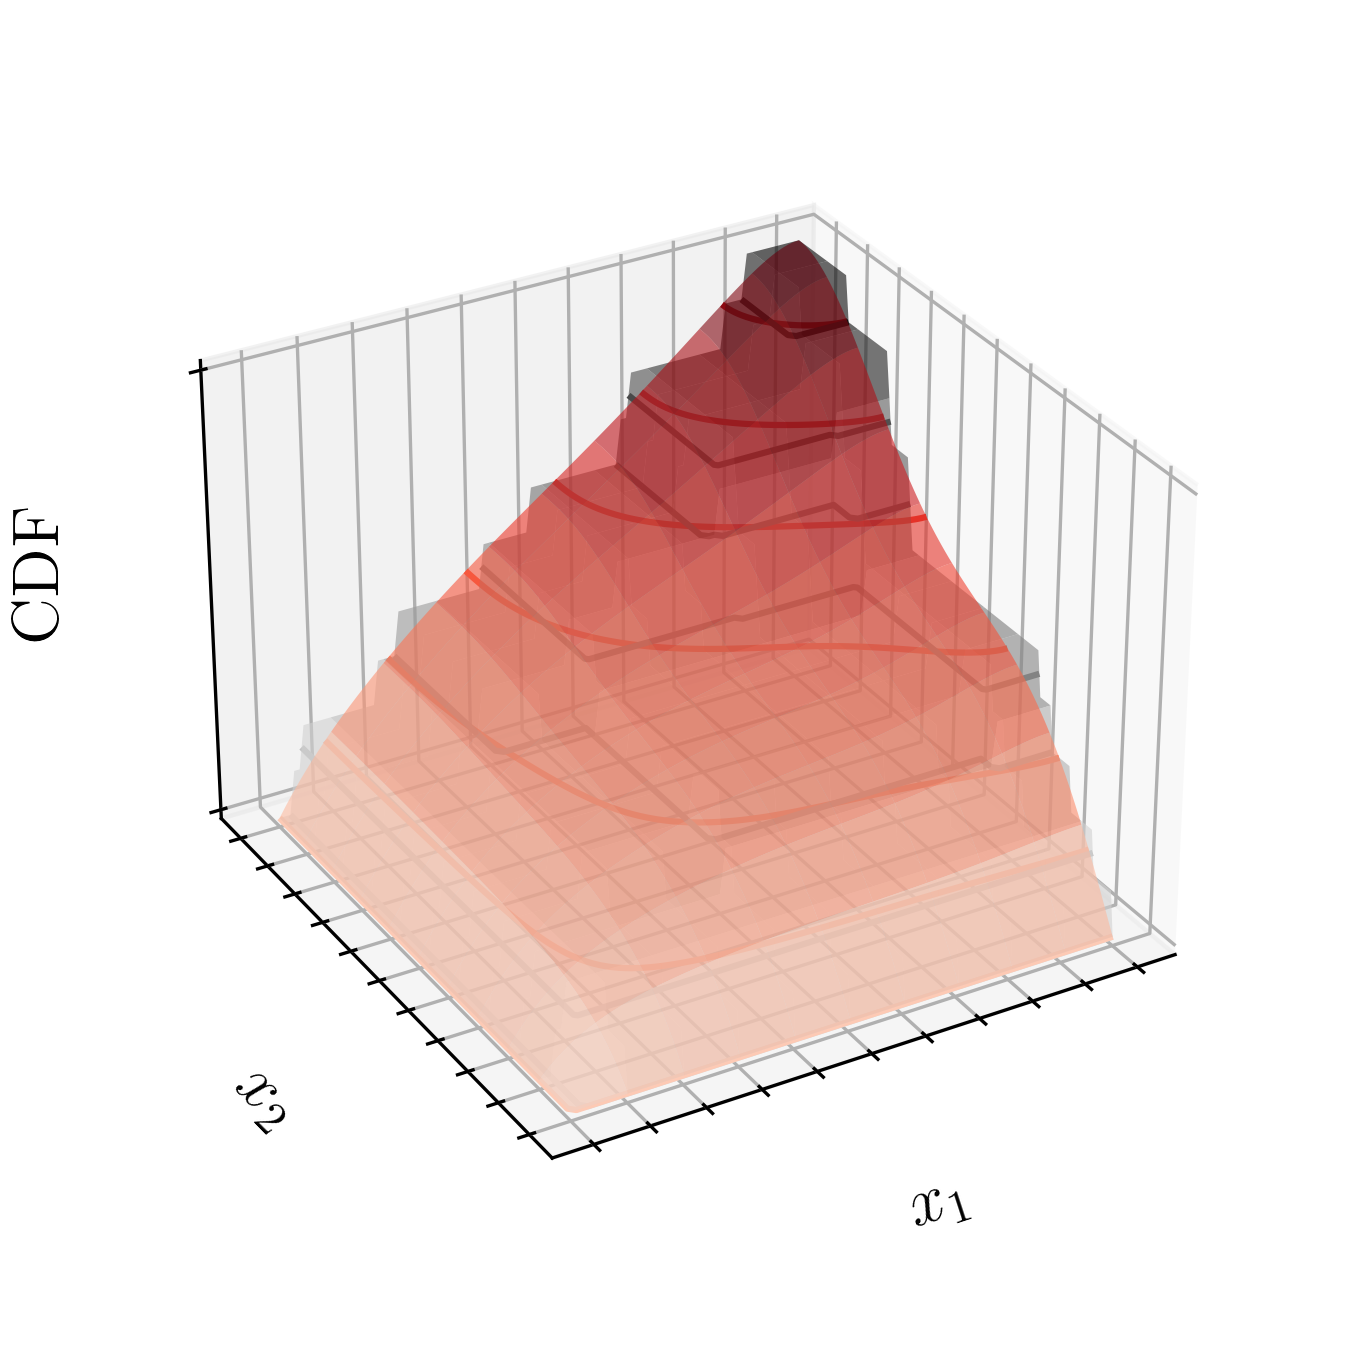
\includegraphics[width=\linewidth]{../numerical_experiments/chapter3/figures/ebc_m10.png}
        \caption{$B_{\bm}(C_n)$ with $(m_1=m_2=10)$.}
    \end{subfigure}
    \begin{subfigure}[b]{0.49\textwidth}
        \centering
        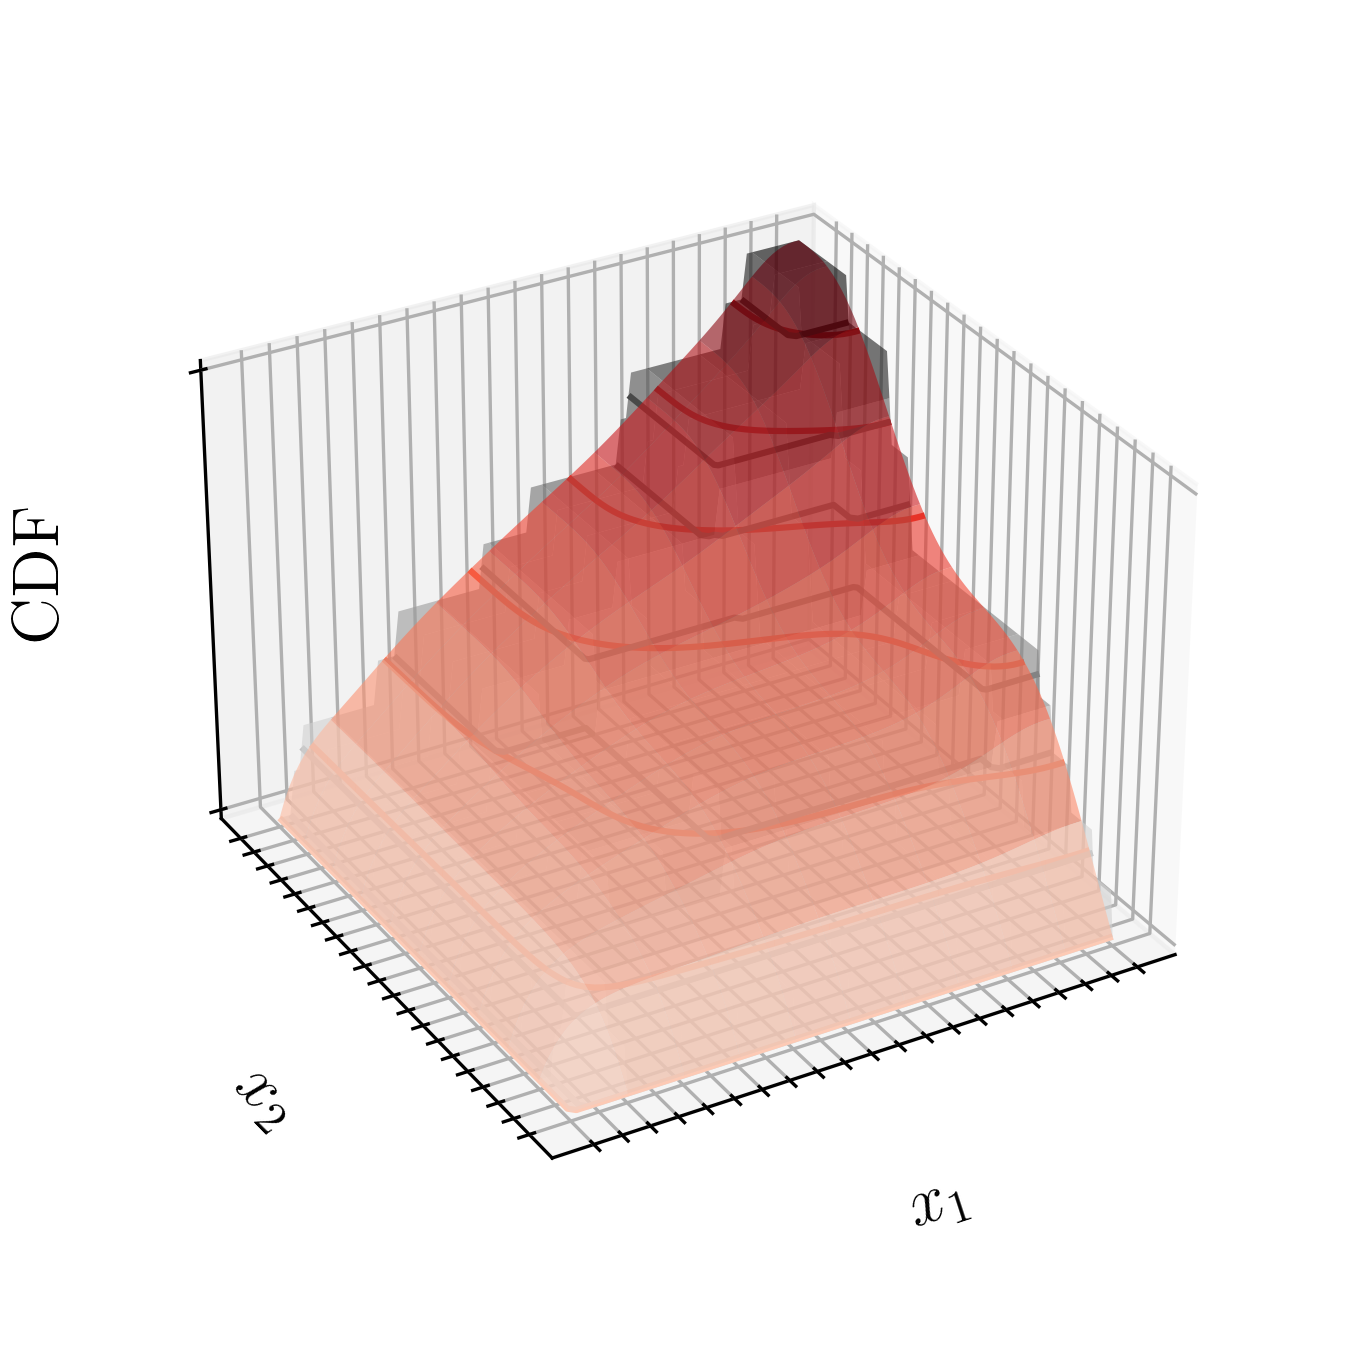
\includegraphics[width=\linewidth]{../numerical_experiments/chapter3/figures/ebc_m20.png}
        \caption{$B_{\bm}(C_n)$ with $(m_1=m_2=20)$.}
    \end{subfigure}
    \centering
    \caption{Bernstein approximations of the empirical copula $C_n$ (with size $n=10$) of a Clayton copula (with parameter $\theta=2.5$). The polynomial orders are assumed equal in the two dimensions $m_1=m_2\in\{3, 10, 20\}$.}
    \label{fig:ebc_illustration}
\end{figure}

\newpage
%============================================================%
%============================================================%
\section{\textit{Copulogram}: a tool for multivariate data visualization}\label{sec:copulogram}
%============================================================%
%============================================================%
In statistics, data visualization offers a wide set of tools to analyze data. 
Multivariate data visualization is of great help to apprehend problems with dimension higher than two. 
In the context of continuous variables, let us consider the $n$-sized sample $\bX_n = \left\{\bx^{(1)}, \dots, \bx^{(n)}\right\} \sim \bX \in \iD_{\bx}\subseteq\R^d$. 
The marginal samples of $\bX_n$ are denoted by $X_{n, j} = \{x_j^{(1)}, \dots, x_j^{(n)}\}, j\in \{1, \dots, d\}$.

Various techniques exist to represent multivariate data, such as the ``parallel coordinate plot'', also called ``cobweb plot'' (see e.g., \citealp{heinrich_2013_cobweb}). 
For each sample $\bx^{(i)} \in \bX_n$, this plot draws a line passing by the values of $\bx^{(i)} = [x_1^{(i)}, \dots, x_d^{(i)}]$. 
This representation was used in sensitivity analysis to illustrate the connections between a set of inputs and an output, however, it does not provide a good representation of the dependence structure between the inputs. 

%============================================================%
\subsection{From the pairwise plot to the copulogram}
%============================================================%
Alternatively, the ``pairwise plot'', also named ``generalized draftsman plot'', was initially introduced by \citet{hartigan_1975_splom} to draw a matrix of scatter-plots between all the pairs of marginal samples $\{X_{n, i}, X_{n, j}\}, i \ne j \in \{1, \dots, d\}^2$. 
Because of the symmetry, the pairwise plot is usually represented on the lower triangle of the matrix. 
Later on, statisticians improved the pairwise plot by adding a histogram (or KDE) of the marginal samples $X_{n, j} j \in \{1, \dots, d\}$ on the diagonal. 
Additionally, the upper triangle was completed with the values of linear correlation for each pairs of marginal sample $\{X_{n, i}, X_{n, j}\}, i \ne j$. 
This matrix of correlation coefficients is also know as ``correlogram''. 
Altogether, this matrix plot became known as the ``scatter plot of matrices'' (SPLOM). 

However, the linear correlation coefficient is known to give a poor description of the dependence in nonlinear cases. 
When analysis a continuous sample $\bX_n \sim \bX$, the Sklar theorem states that the dependence structure within the random vector $\bX$ has a unique expression with its $d$-copula $C$. 
As mentioned in Section~\ref{sec:copula_prelims}, the component wise normalized ranks of the original sample $\bX_n$ define the empirical copula density $c_n$ (converging towards $C$ as $n$ increases).

To the best of our knowledge, the \textit{copulogram} is a new multivariate data visualization tool improving the SPLOM by representing the empirical copula density $c_n$ on the upper triangle of the matrix plot. 
This plot is an empirical decomposition of a multivariate sample in the vein of the Sklar theorem between marginals on the diagonal and copula on the upper triangle.

%============================================================%
\subsection{Implementation in a Python package}
%============================================================%

An open-source implementation is proposed in the python package \href{https://github.com/efekhari27/copulogram}{\texttt{copulogram}}. 
This code mostly relies on the Python package for data visualization \href{https://seaborn.pydata.org/}{\texttt{seaborn}} \citep{waskom_2021_seaborn}. 
The developments are tracked and archived in a GitHub repository\footnotemark and the package can be installed from the package-management system ``PyPI''. 

Multiple visual options are offered by the \texttt{copulogram} package, as illustrated in the GitHub repository. 
For example, the user can represent the univariate samples on the diagonal, or the bivariate samples in the triangles with kernel density estimation.  
Categorical variables can be used to assign different colors depending on the data class. 
The colors can also vary depending on a continuous variable after defining a mapping between the values of this variable and a set of color (also called colorbar).


\footnotetext{GitHub repository: \url{https://github.com/efekhari27/copulogram}}




\subsubsection{Example \#1: Iris flower dataset}
%------------------------------------------------------------%

The first example illustrates the copulogram on a widely used dataset in the machine learning community. 
The iris flower dataset was first introduced by Fisher and became a reference dataset for classification techniques. 
In the following lines of Python code, the dataset is loaded and the copulogram package is used to draw the new plot. 
The resulting copulogram applied to the iris flower data is represented in \fig{fig:iris_copulogram}. 
\lstset{style=mystyle, language=python}
%
\begin{lstlisting}
    #!/usr/bin/python3        
    import seaborn as sns
    import copulogram as cp
    data = sns.load_dataset("iris")
    copulogram = cp.Copulogram(data)
    copulogram.draw(hue="species")
\end{lstlisting}
%
Since this data mostly presents linear dependencies, the copulogram is not very instructive. 
In other cases, the role of the dependence in the joint distribution is more important.



\subsubsection{Example \#2: Ishigami function}
%------------------------------------------------------------%

The Ishigami function is commonly used as a benchmark problem for global sensitivity analysis (GSA): 
\begin{equation}
    y = g(x_1, x_2, x_3) = \sin(x_1) + 7 \, \sin(x_2)^2 + \frac{x_3^4 \, \sin(x_1)}{10}.
\end{equation}
This uncertainty quantification problem considers an independent random input vector $\bX=\prod_{j=1}^{3} X_j$. 
While the marginals in GSA benchmarks are usually assumed to be uniform, they will be considered Gaussian hereafter to distinguish the different elements of the joint distribution. 
Therefore, let us define $X_j\sim \iN(0, 1) \forall j \in \{1, 2, 3\}$. 
In this setup, the random inputs are independent but they each present interesting dependencies with the random output $Y=g(\bX)$.

A Monte Carlo sample with size $n=10^3$ is generated, $\bX_n \simiid \bX$, and evaluated such that $Y_n=g(\bx_n)$.  
The copulogram of the input-output sample $(\bX_n, Y_n)$ is represented in \fig{fig:ishigami_copulogram}. 
As expected, the scatter-plots between the inputs in the upper triangle are uniform (representing an independent density copula). 

In GSA, the work of \citet{poczos_2012_copulaMMD} studied the discrepancy between the empirical density copula $c_n(X_j, Y), j \in \{1, \dots, d\}$ and the independent copula to qualitatively assess the importance of $X_j$.  
In the same vein, the paper of \citet{plischke_2019_copulaGSA} attempted to formalize a link between different GSA approaches based on copulas and to quantitative approaches as the Sobol' indices. 

\begin{figure}
    \centering
    \quad\qquad\qquad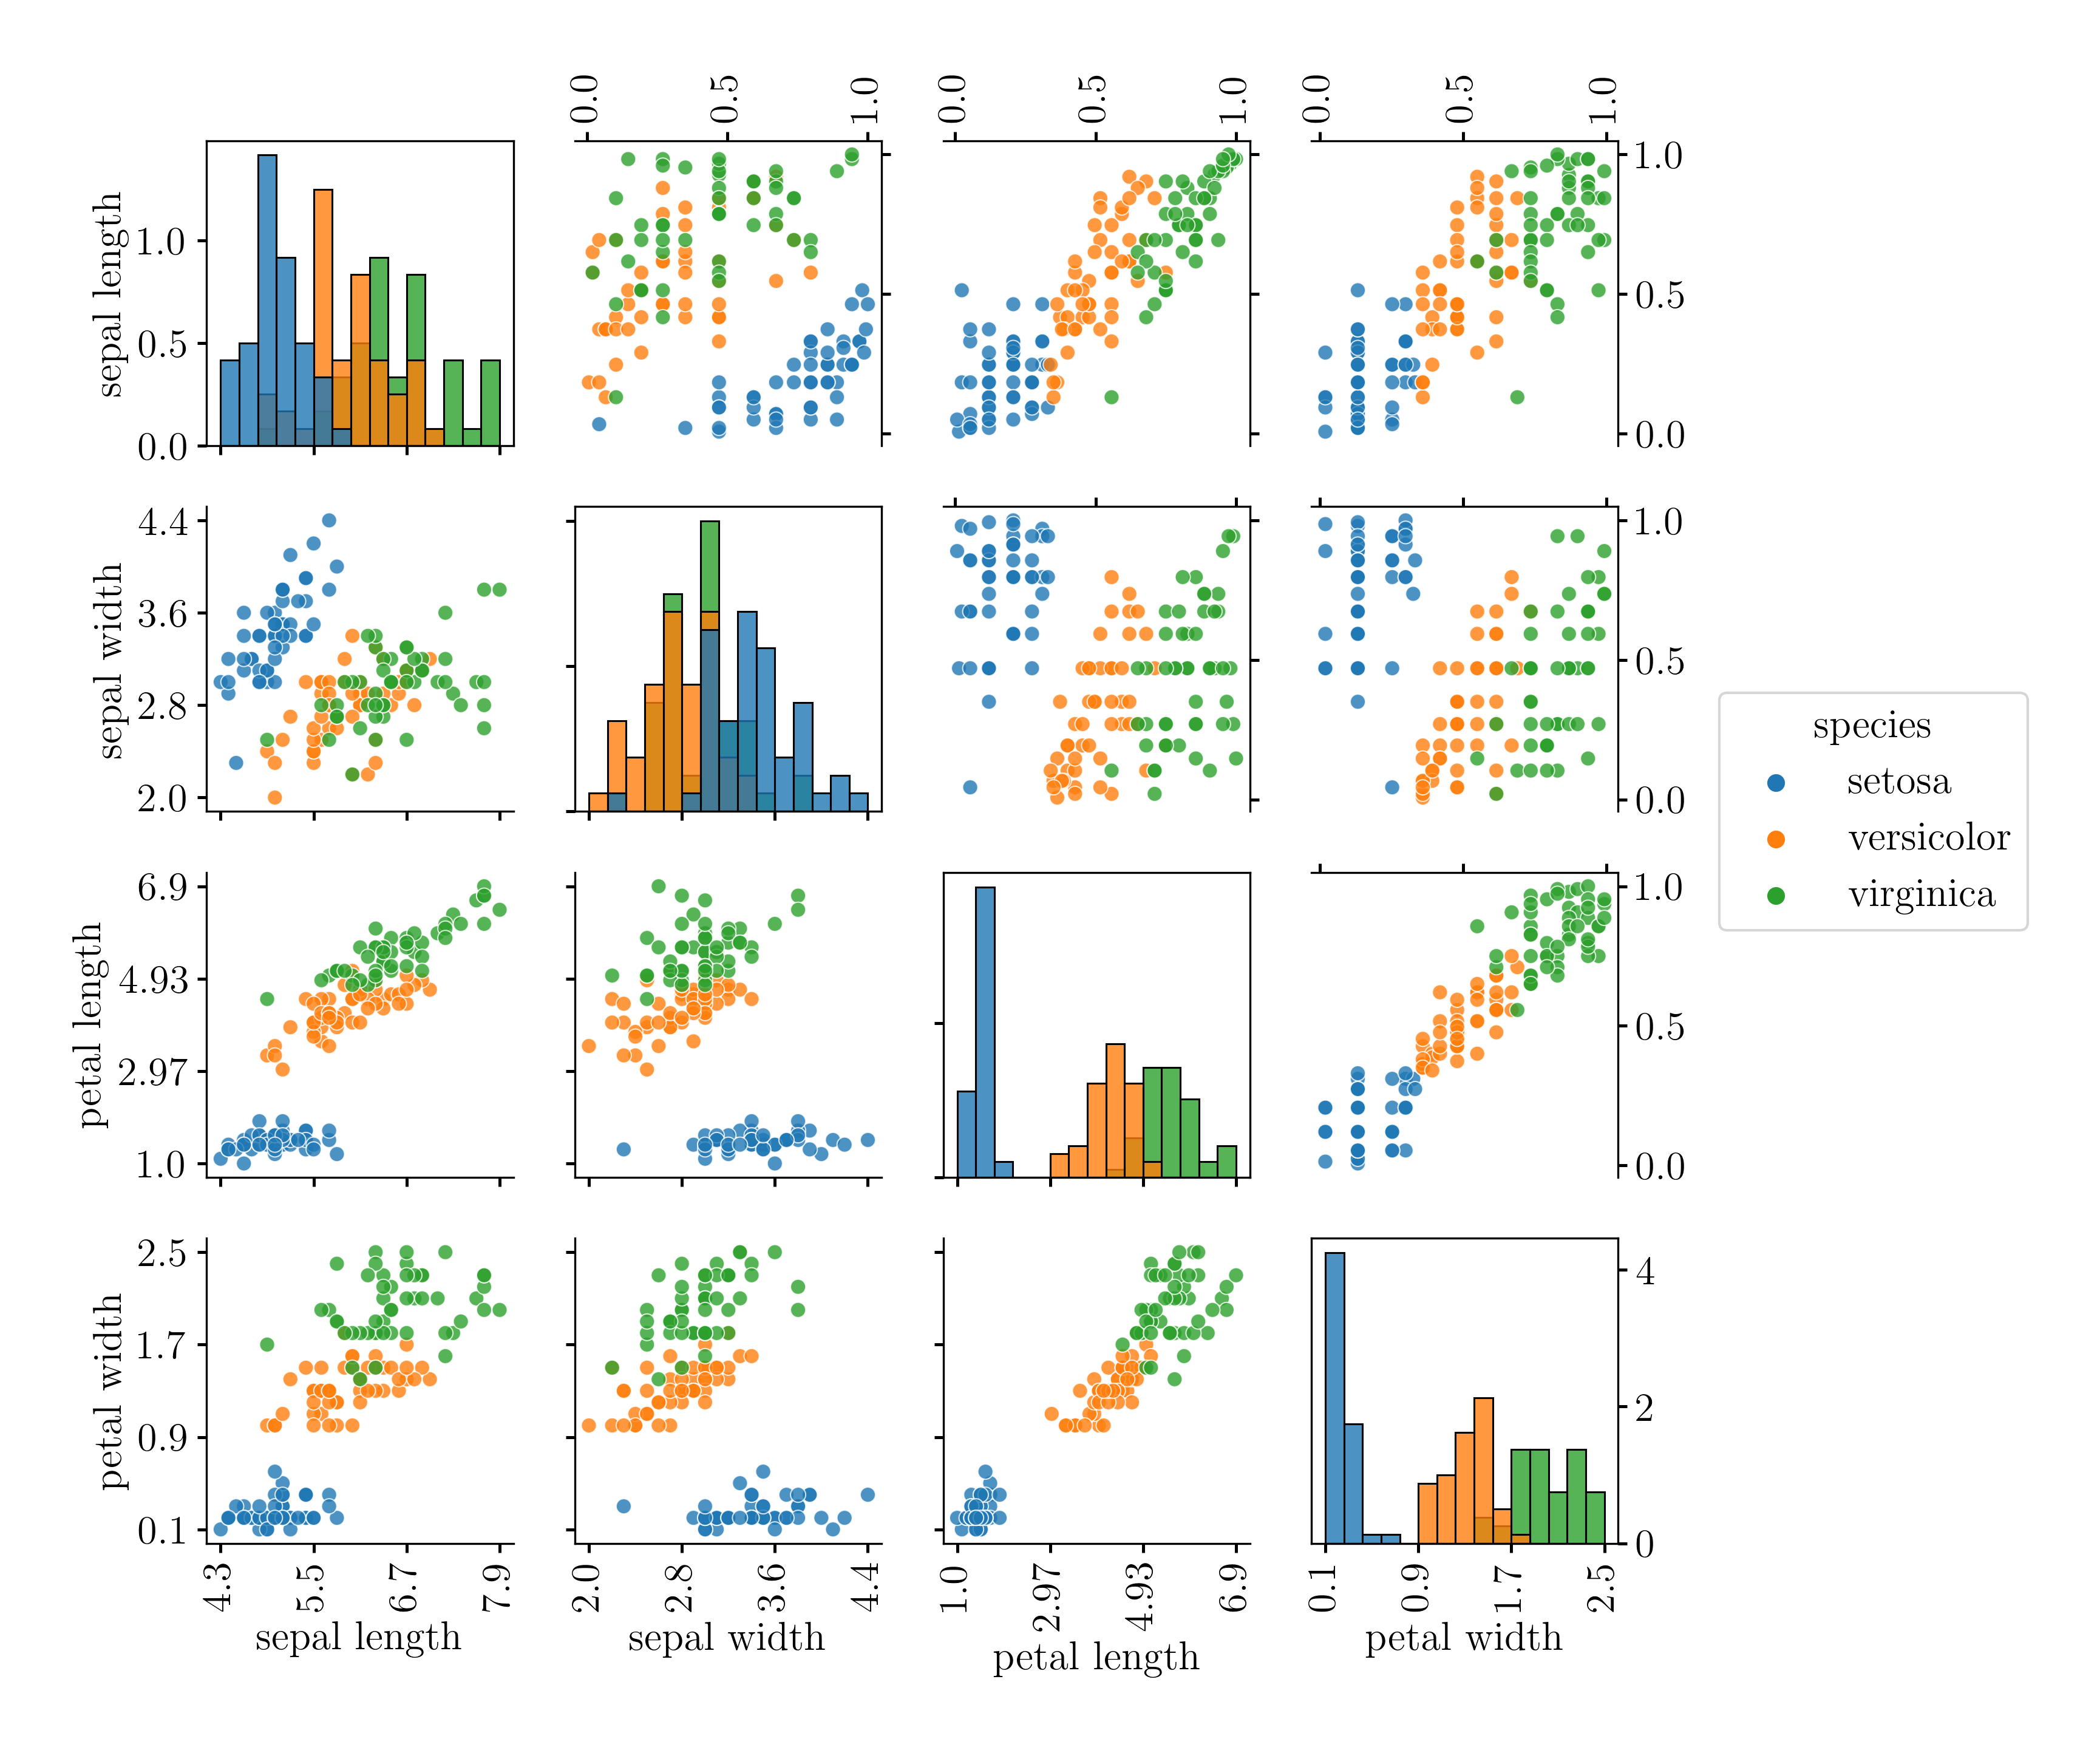
\includegraphics[width=0.82\textwidth]{../numerical_experiments/chapter3/figures/iris_copulogram.png}
    \caption{Copulogram of the iris flower dataset with colors assigned by the iris species.}
    \label{fig:iris_copulogram}
\end{figure}

\begin{figure}
    \centering
    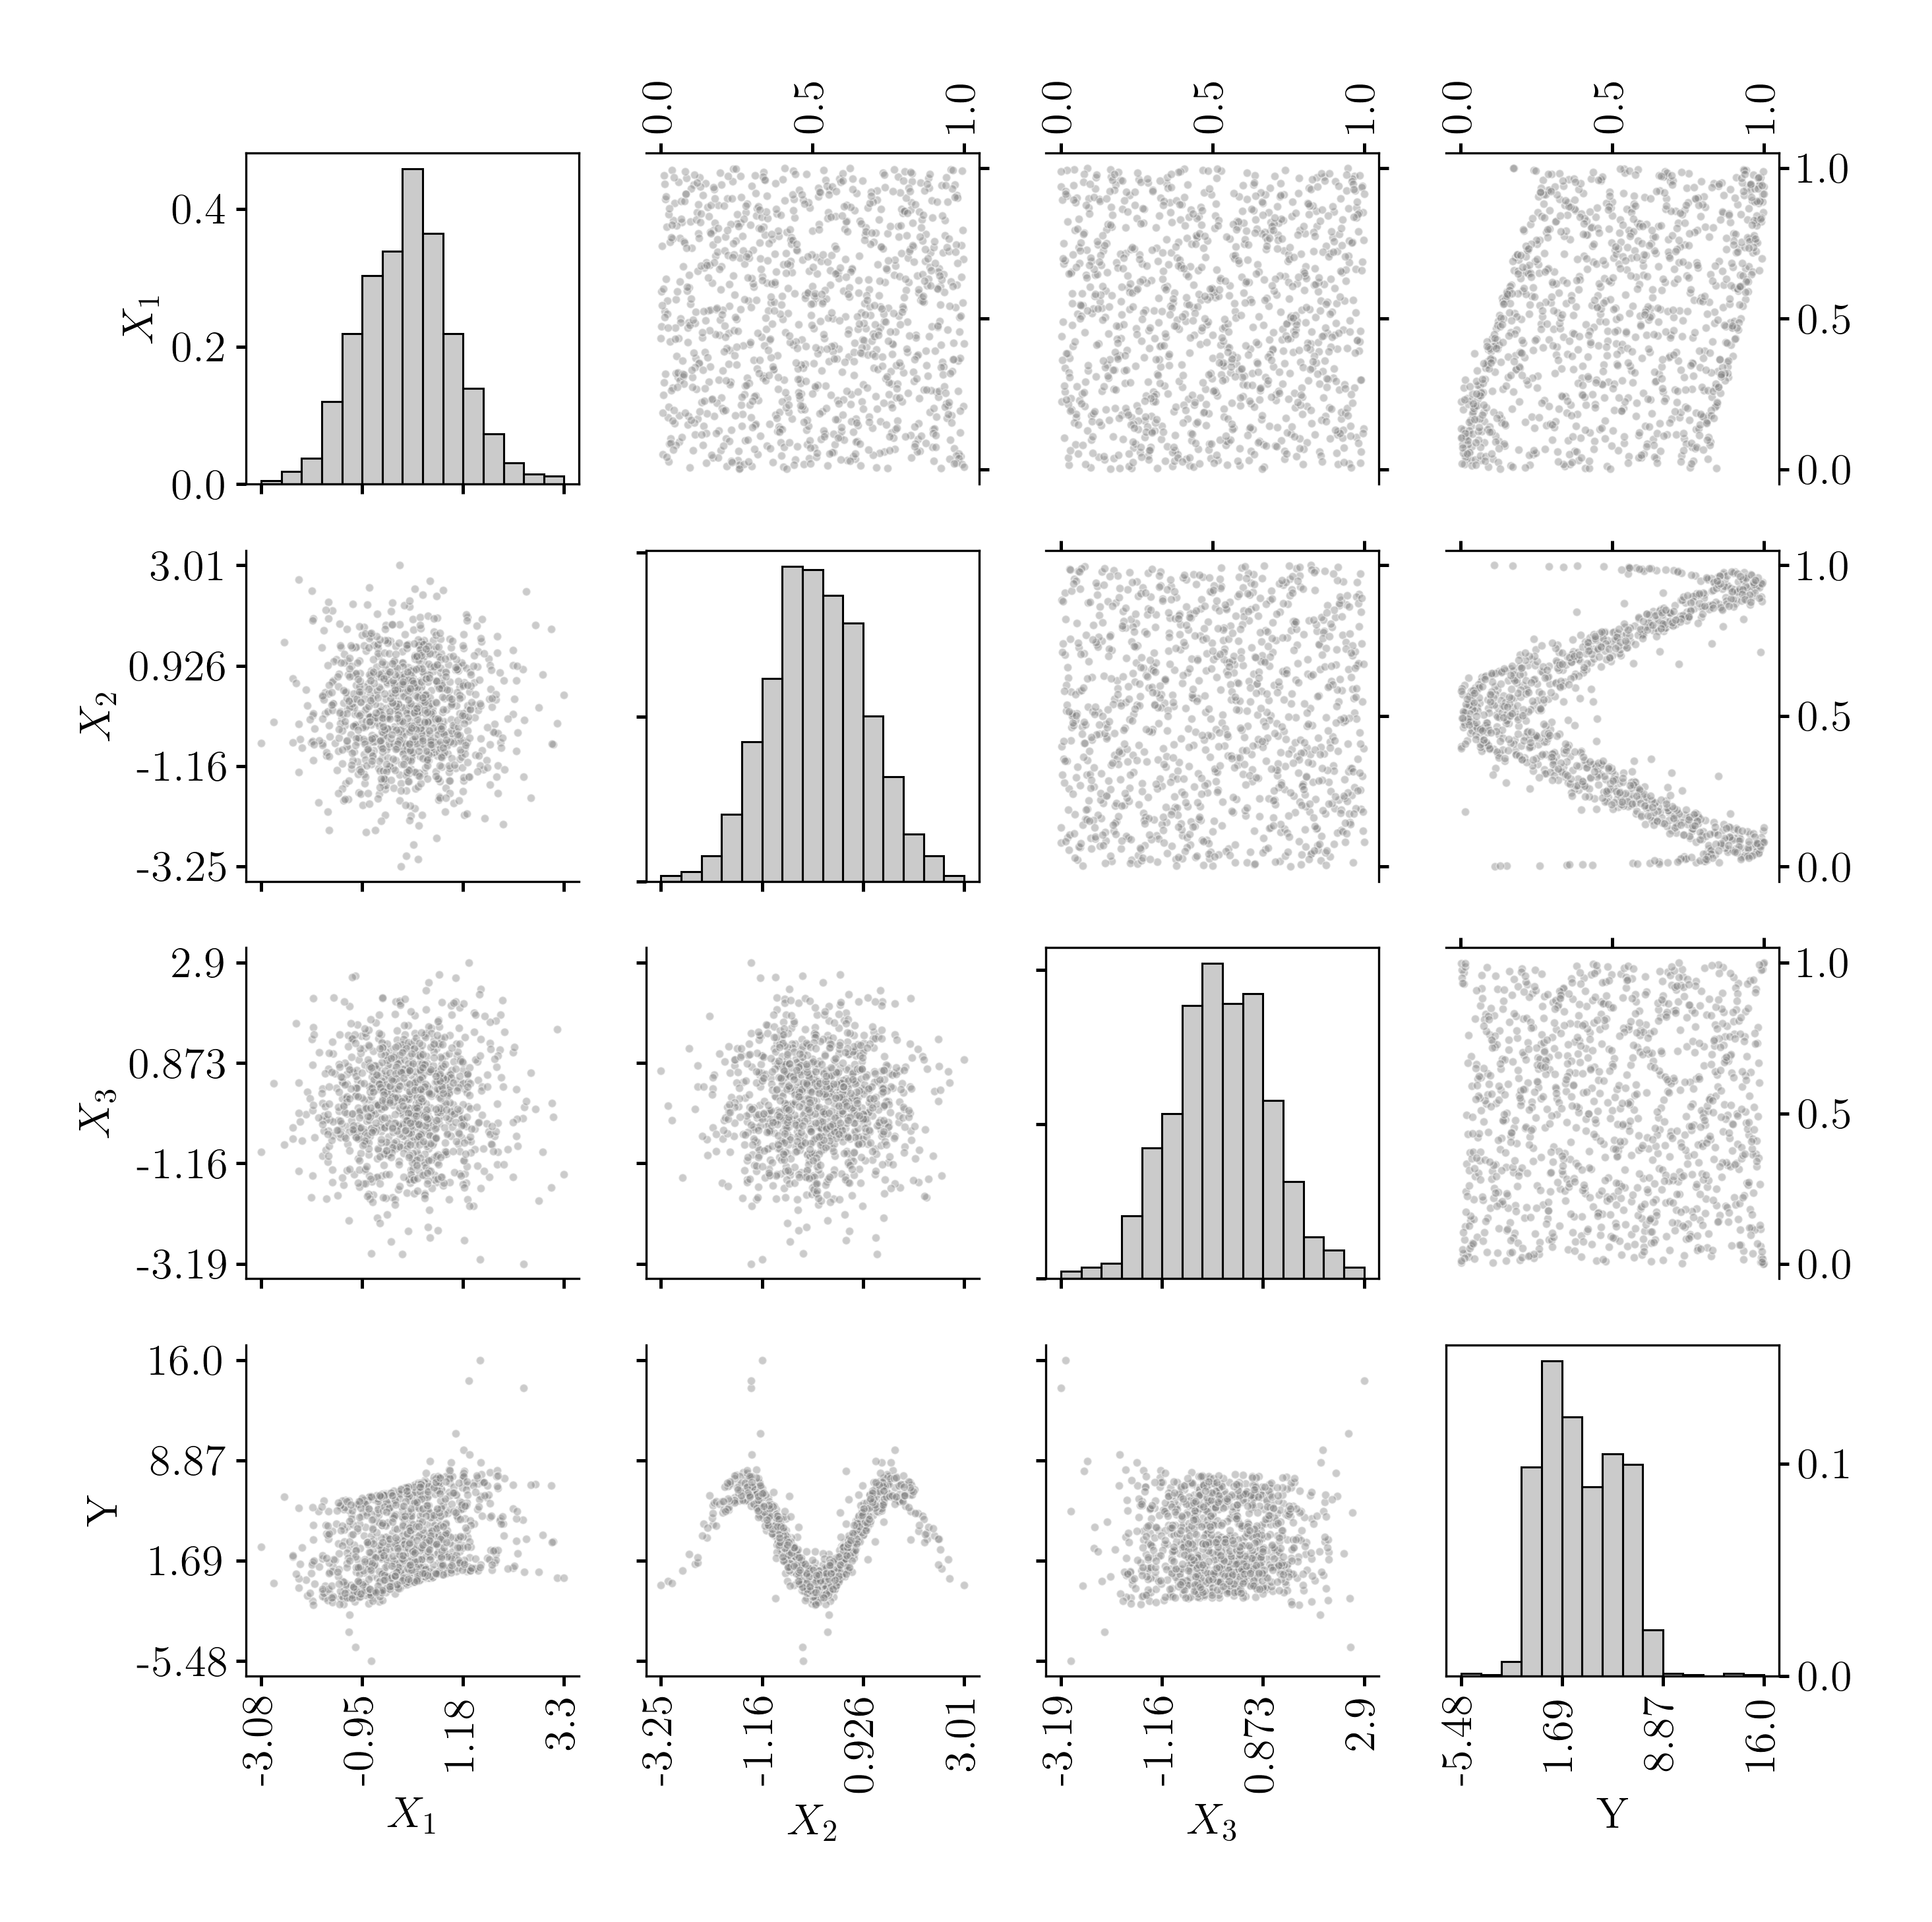
\includegraphics[width=0.7\textwidth]{../numerical_experiments/chapter3/figures/ishigami_copluogram.png}
    \caption{Copulogram of Monte Carlo sample (with size $n=10^3$) of the inputs and outputs of the modified Ishigami problem.}
    \label{fig:ishigami_copulogram}
\end{figure}



\newpage
%============================================================%
%============================================================%
\section{Semiparametric inference of the South Brittany metocean conditions} \label{sec:32_inference}
%============================================================%
%============================================================%
Metocean conditions have been long studied in costal and offshore engineering. 
Inferring multivariate probabilistic models on metocean data became essential in wind energy. 

Numerous approaches are proposed in the literature to fit a model on environmental data. 
Among them, let us mention the use of parametric methods as the conditional modeling (e.g., \citealt{bitner_2015_joint,vanem_fekhari_2023}), or the construction of vine copulas (e.g., \citealt{vanem_2016,montes_2016_cvines_metocean,lin_2019_cvines_waves}). 
Nonparametric methods as the KDE were also applied in this context (e.g., \citealt{han_2018_kde_metocean}). 
The nonparametric techniques generally struggle to model the distributions' tails, even if the tails are essential to qualify structures for ultimate events. 
However, they are highly flexible and often easier to implement than parametric methods.

In this section, a semiparamertic inference strategy is presented, composing some well-known parametric models for the marginals (e.g., Weibull distribution for the wind speed), with a highly flexible dependence modeling by the EBC. 
A metocean dataset is used to showcase the empirical Bernstein copula and its representation by the copulogram. 
This dataset from the ANEMOC (Digital Atlas of Ocean and Coastal Sea States atlas, \citealp{raoult_2018_anemoc3}) gathers 32 years of preprocessed data 
(at an hourly resolution) from a location off the coast of South Brittany, France. 
A subset of $10^4$ points is randomly selected among the ANEMOC data, which will be used to realize the semiparametric inference.

\elias{add the repo for the study}

%============================================================%
\subsection{Inference of the marginals}\label{sec:marginal_inference}
%============================================================%

The variables studied to describe the environmental conditions match the ones defined in Table~\ref{tab:envi_variables}. 
Unfortunately, the turbulence is provided by the ANEMOC database and is therefore not fitted. 
A straightforward inference is performed on the data, resulting in the models presented in Table~\ref{tab:sb_marginal_fit}.
The wind and wave directions are fitted by KDE to catch their multimodal behavior while the other variables by MLE on various parametric models. 
Note that some variations of KDE with kernels specific to circular data could be interesting to ensure the continuity of the model at the bounds \citep{bai_1989_directional_kde}. 

The results of the marginals' inferences, plotted in \fig{fig:marginals_sb} against histograms, are visually satisfying. 
Statistical testing is not necessary in our case since the actual topic of discussion is related to the inference of the dependence. 
Considering these marginals, a study of the copula inference can be developed. 


\begin{table}
    \centering
    \begin{tabular}{llll}
        \hline
        {\it Name}              & {\it Notation}            & {\it Fitted model}                            & \textit{KS p-value ($\alpha$= 5\%)} \\
        \hline
        Wind speed              & $U$                       & Weibull ($\beta=11.4, \alpha=2.2, \gamma=0$)  & 0.238     \\
        Wind direction          & $\theta_{\mathrm{wind}}$  & KDE                                           & --        \\ 
        Significant wave height & $H_s$                     & Inverse Normal ($\mu=2.3, \lambda=6.8$)       & 0.533     \\
        Wave period             & $T_p$                     & Weibull ($\beta=9.3, \alpha=3.3, \gamma=2$)  & 0.00021   \\
        Wave direction          & $\theta_{\mathrm{wave}}$  & KDE                                           & --        \\
        \hline
    \end{tabular}
    \caption{Marginal inference results of the South Brittany metocean data.}
    \label{tab:sb_marginal_fit}
\end{table}

\begin{figure}
    \centering
    \begin{subfigure}[b]{0.32\textwidth}
        \centering
        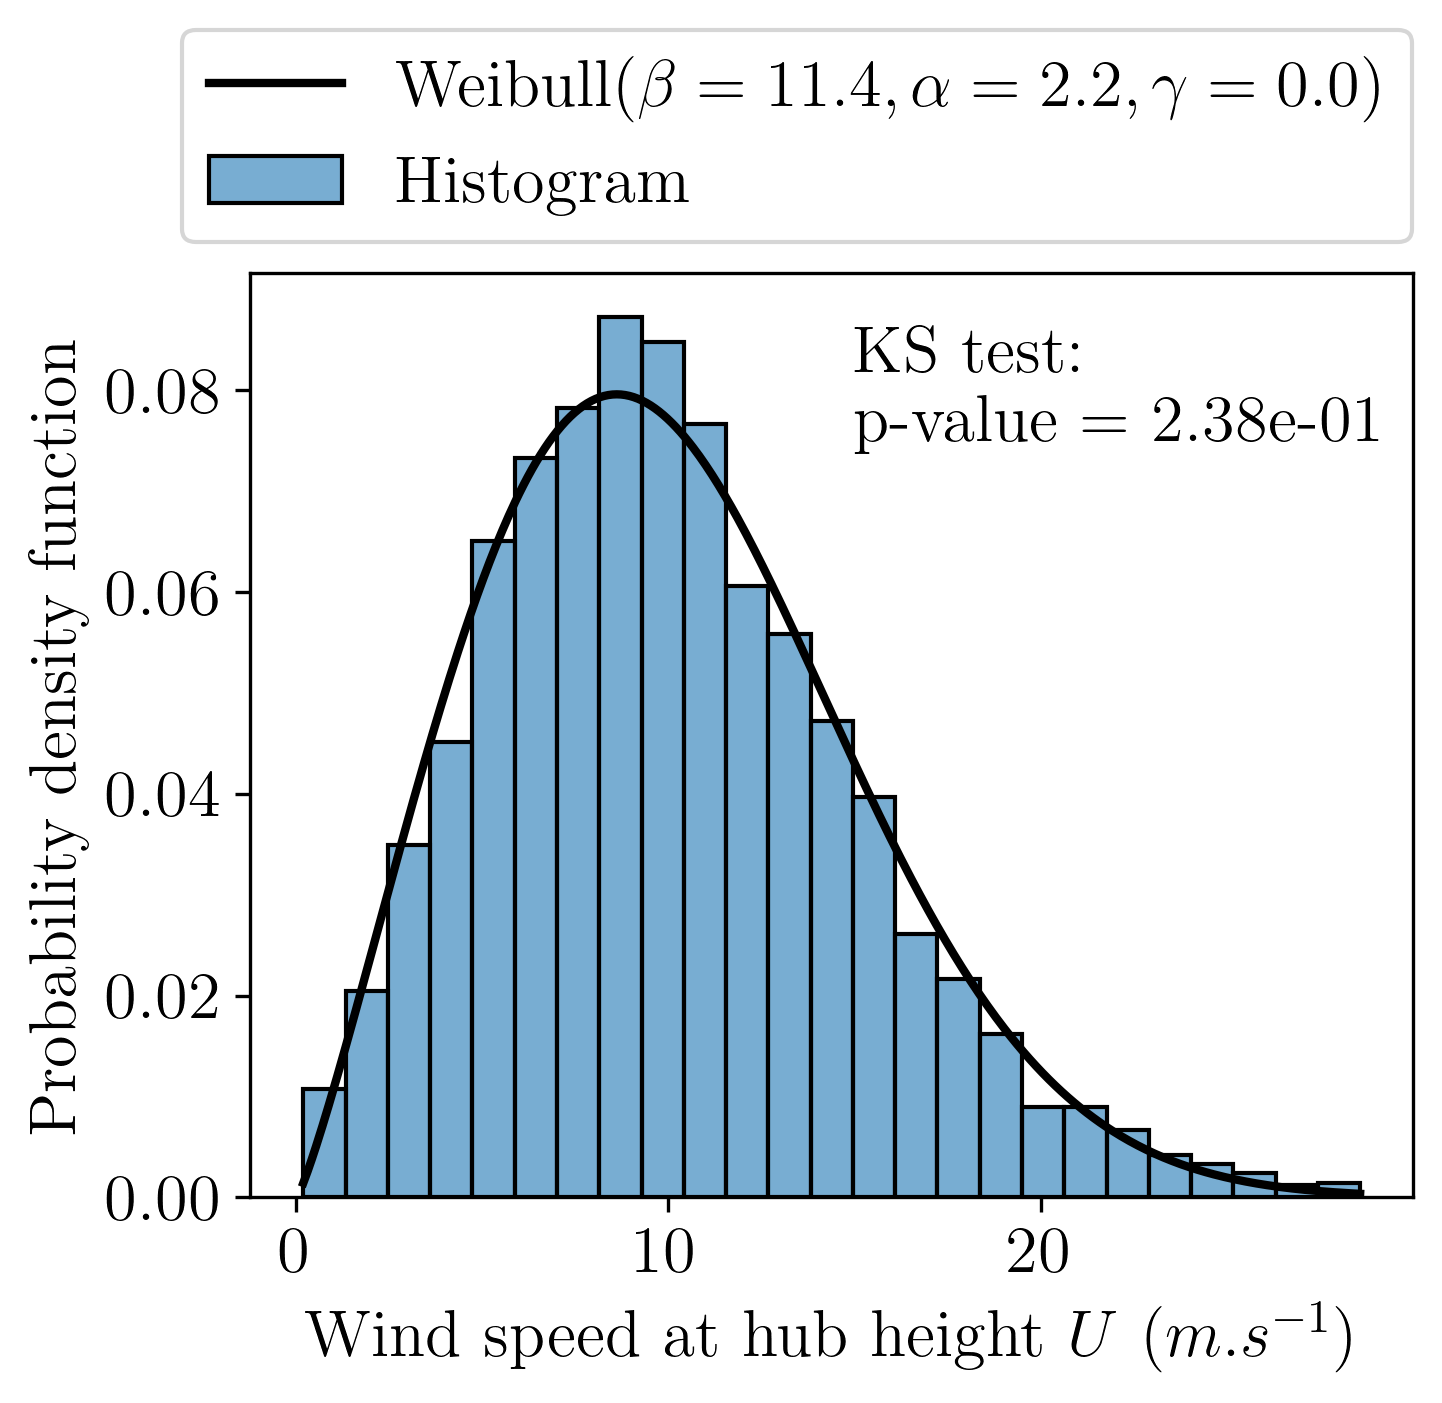
\includegraphics[width=\linewidth]{../numerical_experiments/chapter3/figures/free_wsp_distribution_SB.png}
        \caption{Wind speed $U$.}
    \end{subfigure}
    \begin{subfigure}[b]{0.32\textwidth}
        \centering
        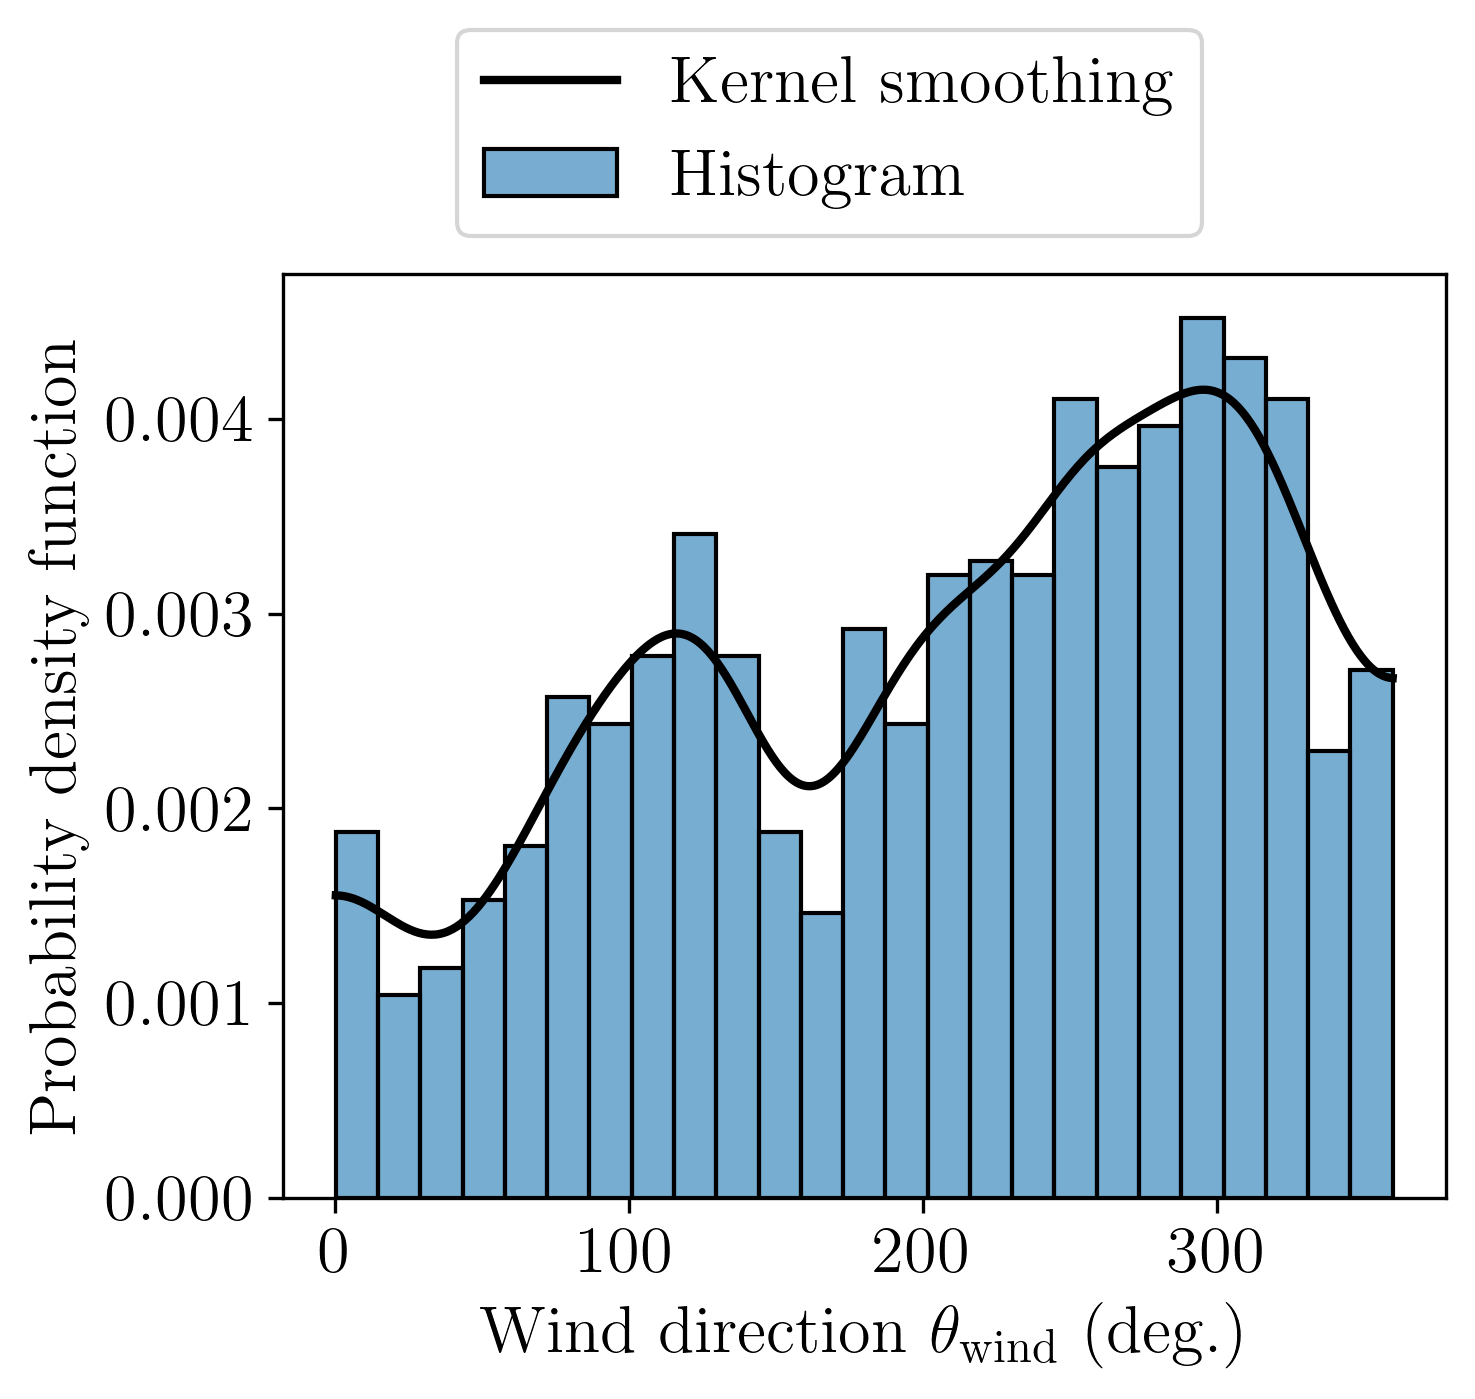
\includegraphics[width=\linewidth]{../numerical_experiments/chapter3/figures/wind_dir_distribution_SB.png}
        \caption{Wind direction $\theta_{\mathrm{wind}}$.}
    \end{subfigure}
    \\
    \begin{subfigure}[b]{0.32\textwidth}
        \centering
        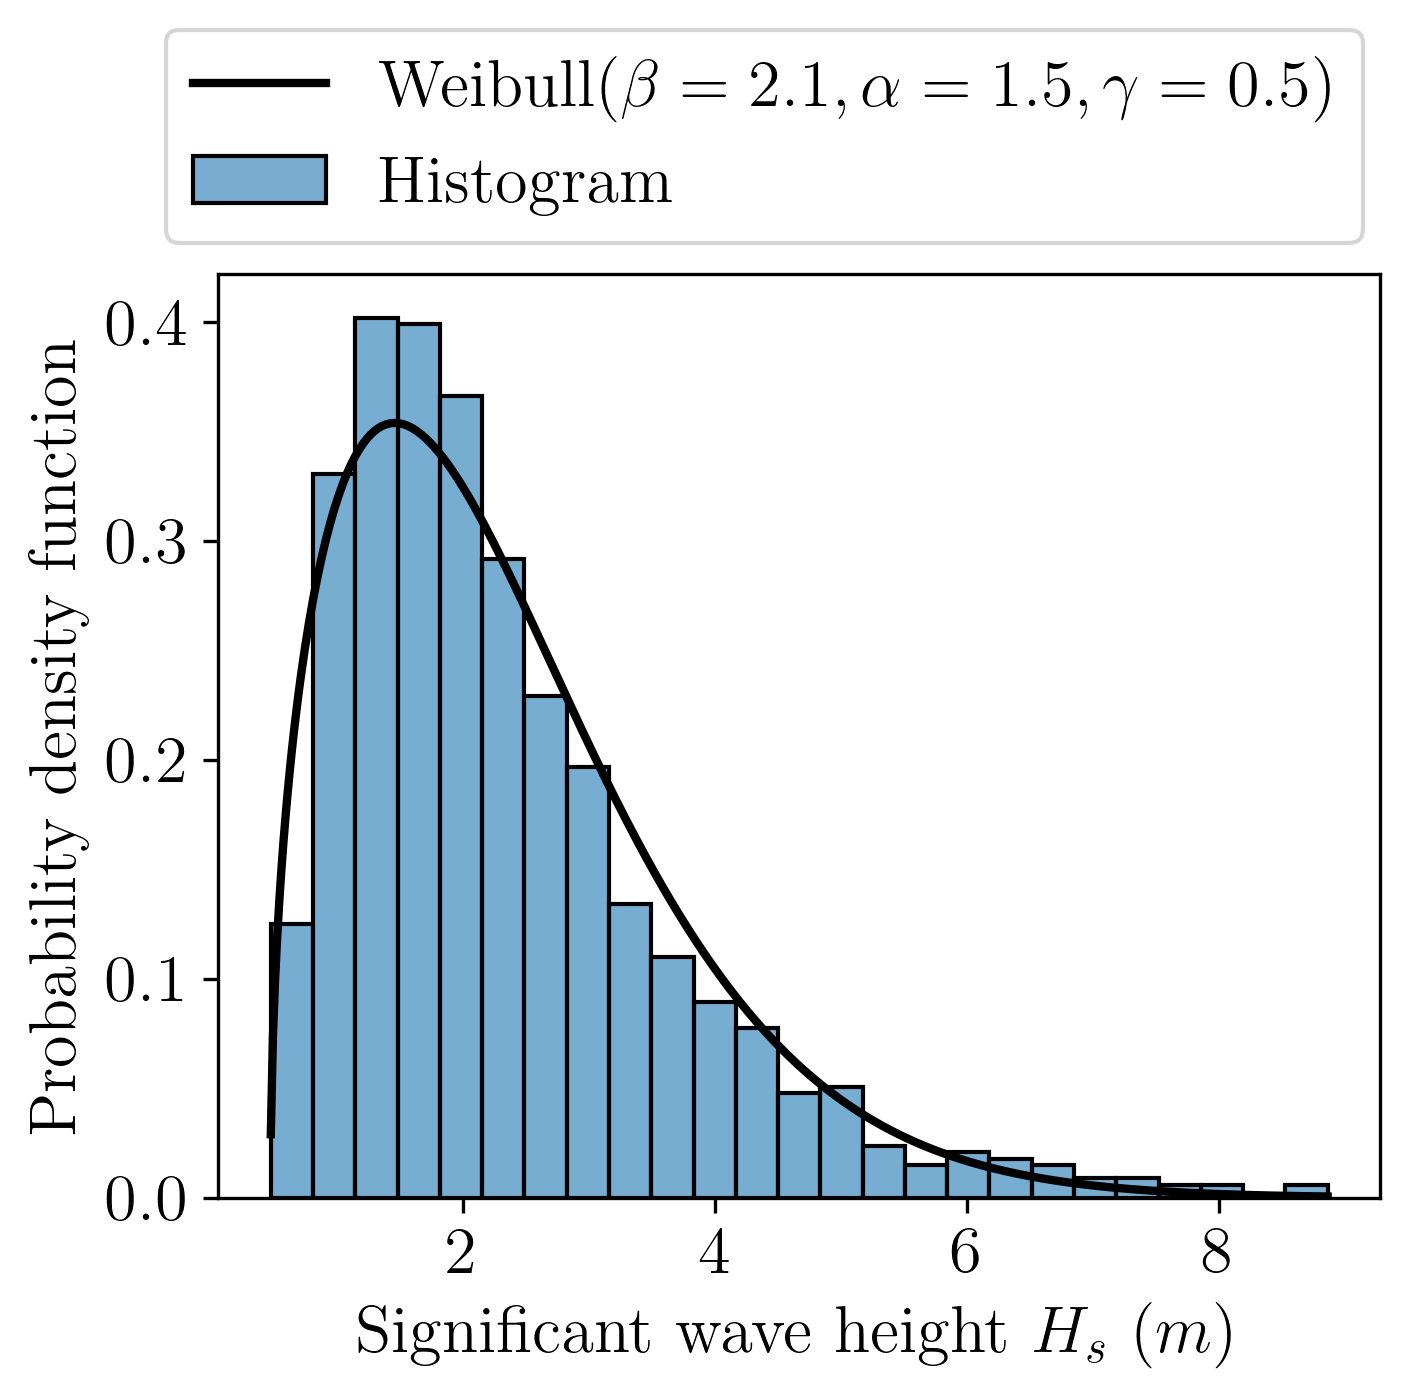
\includegraphics[width=\linewidth]{../numerical_experiments/chapter3/figures/Hs_distribution_SB.png}
        \caption{Significant wave height $H_s$.}
    \end{subfigure}
    \begin{subfigure}[b]{0.32\textwidth}
        \centering
        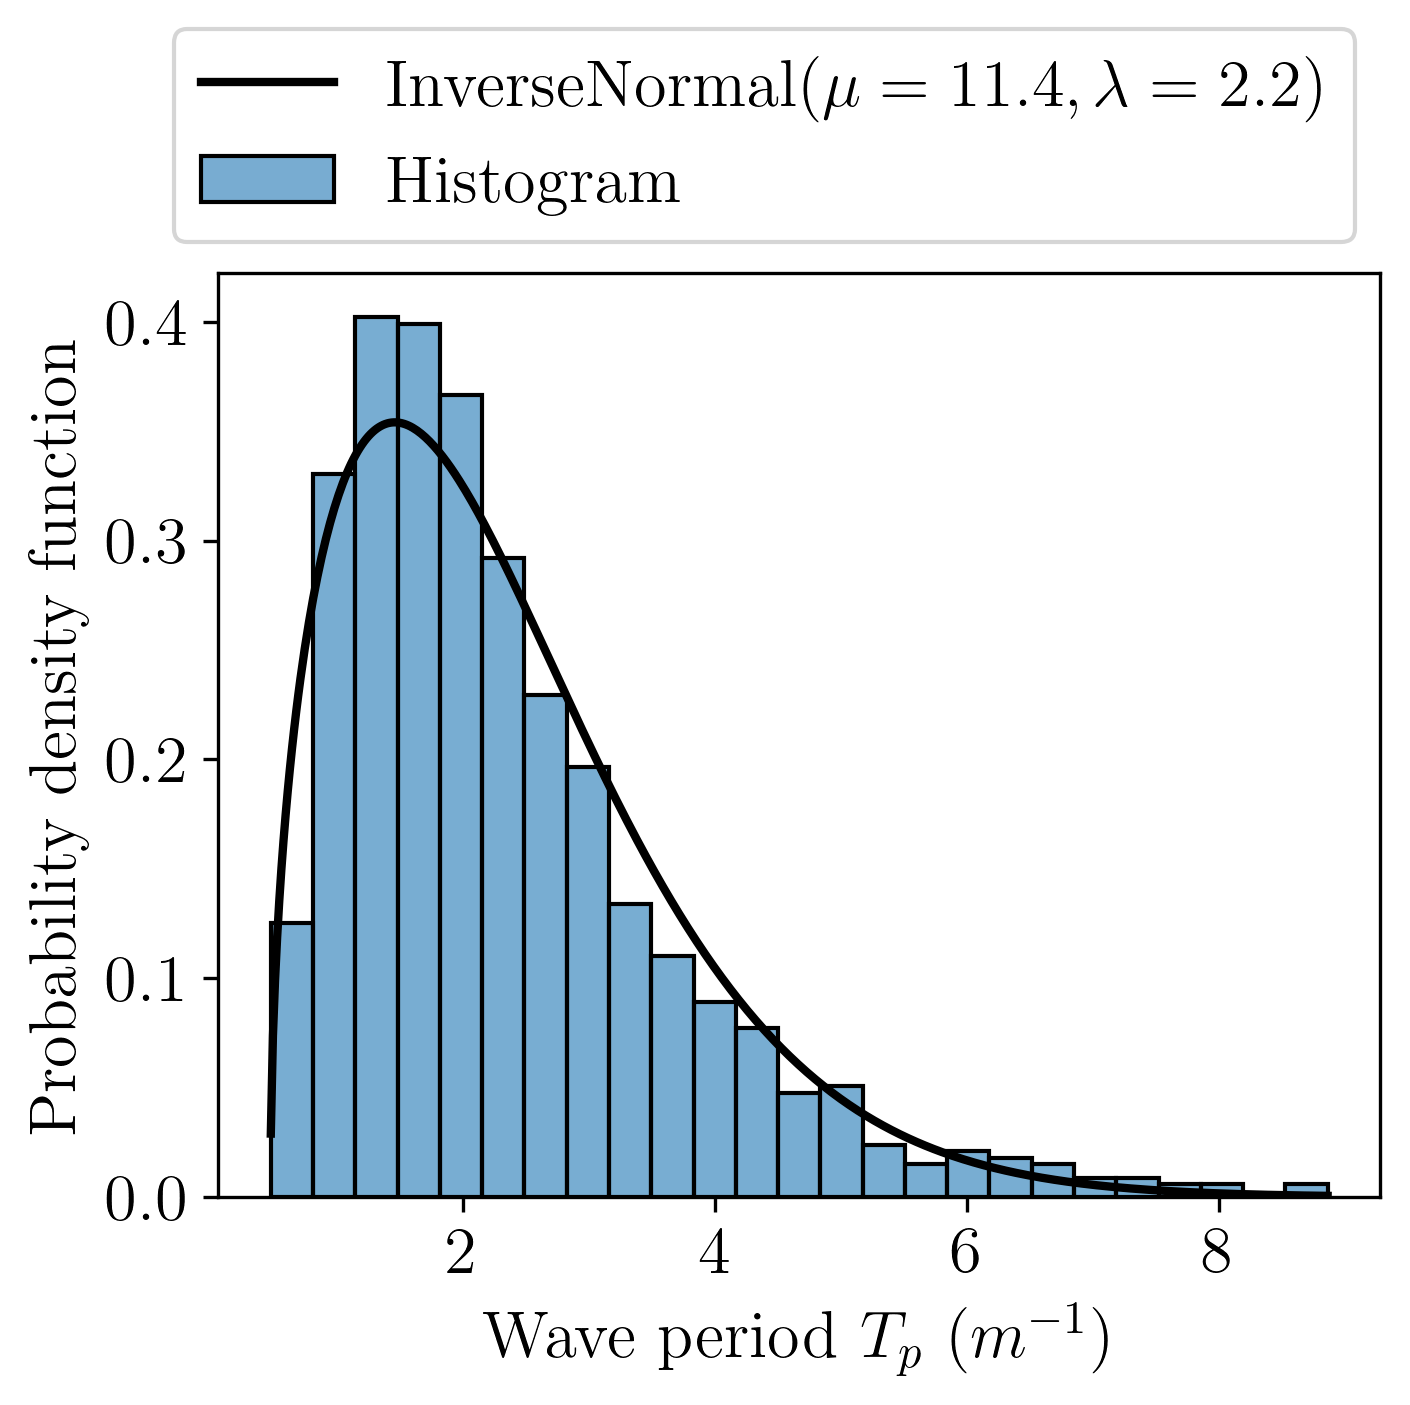
\includegraphics[width=\linewidth]{../numerical_experiments/chapter3/figures/Tp_distribution_SB.png}
        \caption{Wave period $T_p$.}
    \end{subfigure}
    \begin{subfigure}[b]{0.32\textwidth}
        \centering
        \includegraphics[width=\linewidth]{../numerical_experiments/chapter3/figures/wave_dir_distribution_SB.png}
        \caption{Wave direction $\theta_{\mathrm{wave}}$.}
    \end{subfigure}
    \caption{Marginal inference results of the South Brittany metocean data.}
    \label{fig:marginals_sb}
\end{figure}

\newpage
%============================================================%
\subsection{Nonparametric inference of the dependence}
%============================================================%

The aim of this section is to complete the set of marginals fitted previously by the inference of a copula. 
A nonparametric estimation using the empirical Bernstein copula is studied in this section. 
To validate the goodness-of-fit of the EBC, the ANEMOC dataset (with size $N=10^4$) is randomly split into two:
a learning set $\bX_n$ and a validation set $\bX_n'$. 
A joint distribution $\what{F_\bX}$ is then build using $\bX_n$, by combining the marginals fitted earlier with an empirical copula $B_{\bm}(C_n)$, such that: 
\begin{equation}
    \what{F_\bX}(\bx) = B_{\bm}(C_n)\left(\what{F_{X_1}}(x_1), \dots, \what{F_{X_d}}(x_d)\right).
\end{equation}
Where $\what{F_{X_j}}$ stand for the model of the marginal $j$, just inferred in Section~\ref{sec:marginal_inference}. 
While $C_n$ is the empirical copula associated with the sample $\bX_n$, and all the polynomial orders of the EBC are equal, $\bm = \{m, \dots, m\}, m\in\N$.

Then, one could compare a sample $\what{\bX_n}$, generated from the fitted joint distribution $\what{F_\bX}$, with the learning set $\bX_n$. 
However, to prevent an overfit from the semiparametric model, the comparison is rather done between $\bX_n$ and the independent validation set $\bX_n'$. 
The statistic used is the maximum mean discrepancy, $\MMD(\what{\bX_n}, \, \bX_n')$, initially introduced for multivariate two-sample testing (a specific presentation of the MMD and its estimation is developed in Appendix~\ref{apx:B}). 
For a given fitted joint distribution, this procedure is repeated 100 times to take into account the sampling variability. 

In \fig{fig:sb_ebc_mmd}, MMD distributions are represented for different values of the EBC polynomial order, with $m\in\{5, 10, 20, 50, 100, 1000\}$. 
The smallest the values of this dissimilarity measure, the closer the samples should be. 
Even if further developments could be implemented to improve the MMD estimation, these results are sufficient to set the EBC tuning at $m=100$. 
Considering this setup, \fig{fig:sb_copulograms} represents the copulogram of a sample $\what{\bX_n}$ (in red), side by side with the copulogram of the learning set $\bX_n$ (in blue).  
This semiparametric approach offers a lot of flexibility, which is essential when inferring such complete dependence structures. 
As any nonparametric method, it should be used with caution when inferring distributions' tails.  


\begin{figure}[h]
    \centering
    \includegraphics[width=0.7\textwidth]{../numerical_experiments/chapter3/figures/SB_MMD_goodness.png}
    \caption{Empirical distributions of the maximum mean discrepancy between the validation sample $\bX'$ and the sample $\what{\bX_n} \simiid \what{F_\bX}$ (repeated for 100 samples $\what{\bX_n}$).}
    \label{fig:sb_ebc_mmd}
\end{figure}


\begin{landscape}
    \begin{figure}
        \begin{subfigure}[b]{0.49\linewidth}
            \centering
            \includegraphics[width=\linewidth]{../numerical_experiments/chapter3/figures/SB_data_copulogram.png}
            \vspace*{2pt}
            \caption{South Brittany ANEMOC data (size $n=5000$).}
        \end{subfigure}
        \begin{subfigure}[b]{0.49\linewidth}
            \centering
            \includegraphics[width=\linewidth]{../numerical_experiments/chapter3/figures/SB_EBC_copulogram.png}
            \caption{Monte Carlo sample (size $n=5000$), generated from the semiparamertic model fitted on the ANEMOC data (EBC $B_{\bm}(C_n)$ with $ \{m_j=100\}_{j=1}^d$).}
        \end{subfigure}
        \vspace*{5pt} 
        \caption{Copulogram of the South Brittany metocean data.}
        \label{fig:sb_copulograms}
    \end{figure}
\end{landscape}




%============================================================%
\subsection{Summary and discussion}
%============================================================%

In this section, a semiparametric inference strategy was illustrated on a metocean dataset from a site off the coast of South Brittany, France. 
This approach is pragmatic and offers a lot of flexibility. 
In our case, the unimodal marginals are fitted by MLE while the multimodal ones are fitted by KDE. 
Considering the complexity of the dependence, the EBC showed interesting results for large size samples. 
It scapacity to extrapolate in the tails could be further studied \citep{heredia_2022_nonparam_copula} but this tool is an appropriate solution for general inference (for example needed for fatigue assessment). 

In the monograph of \citet{joe2011dependence}, the use of nonparametric methods is briefly discussed p.250. 
The author recommends using nonparametric copulas when the marginals are well-behaved, but the dependence structure is nonlinear. 


%============================================================%
%============================================================%
\section{Quantifying and clustering the wake-induced perturbations within a wind farm}
%============================================================%
%============================================================%
\elias{add ref: ``Difference in load predictions obtained with effective turbulence vs. a dynamic wake meandering modeling approach''}

After defining a probabilistic model based on ambient metocean data, the present section studies the impact of the wake on the wind conditions within a farm. 
The wake arises from extracting kinetic energy from the wind, leading to a decrease in wind speed and an increase in turbulence downstream of the turbines. 
Within a wind farm, the wake mostly depends on the turbines' layout, ambient wind speed, and ambient turbulence intensity. 
The resulting heterogeneous wind field in a wind farm can be simulated by numerical models with different fidelities (as discussed in Section~\ref{sec:222}). 

In our case, simplified wake models (sometimes called ``engineering'' models, see e.g., \citealp{doubrawa_2020_benchmark}) are used to simulate the wind speed deficit and the wake added turbulence at each turbine.
To recover a wake perturbed wind distribution at each turbine, the ambient wind distribution is propagated thought a wake model. 
Having different wind distributions naturally impacts the loading and should be considered during fatigue assessment at a farm scale. 
Such heterogeneity is currently not considered by the design load cases from internation standards, deriving from ambient environmental conditions. 

In practice, fatigue assessment on a turbine represents a computational effort. 
Considering a particular wind distribution per turbine (due to the wake) implies to repeat this assessment for every turbine. 
To make the wake consideration tractable at a farm scale, the present section aims at building clusters of turbines similarly affected by the wake. 
Then, fatigue assessment of the farm can be computed on a few turbines, each representing a cluster of turbines facing similar wake-modified wind loading. 
The maximum mean discrepancy (MMD) is used as a statistical dissimilarity measure to compare the perturbed distributions induced by the wake. 

This new approach is applied on a theoretical wind farm representing the recent call for tenders off the coast of South Brittany, France. 
The turbines considered are a modified version of the floating offshore wind turbine (FOWT) IEA-15MW (described in \citealp{kim_natarajan_2022}). 
Figure~\ref{fig:SB-farm} illustrates the layout of the 25 FOWTs modeled in the following, the coordinates are normalized by the rotor's diameter $D$. 
The spacing between turbines in this regular layout is equivalent to seven rotor diameters in the dominant wind direction and five rotor diameters in the orthogonal direction (i.e., crosswind). 


To xxxxx, the present section is structured as follows: 
first the wake model and the corresponding uncertainty propagation are presented, then the MMD is estimated between the resulting empirical distributions, and finally a simple clustering method defines the final clusters and their representative turbines. 
The main conclusion suggests four clusters among the 25 FOWT which can then be used for fatigue assessment of the farm.

\begin{figure}
    \centering
    \includegraphics[width=0.48\textwidth]{part2/figures/WAKE/SB1.png}
    \includegraphics[width=0.4\textwidth]{../numerical_experiments/chapter3/figures/SB_wind_rose.png}
    \caption{South Brittany wind farm layout \elias{redo in high res} (left). South Brittany wind rose from the ANEMOC data (right).}
    \label{fig:SB-farm}
\end{figure}


%============================================================%
\subsection{Uncertainty propagation on a wake model}\label{sec:UQ-wake}
%============================================================%

%------------------------------------------------------------%
\paragraph{Wake model definition}
%------------------------------------------------------------%
Based on the results of previous numerical studies, with either dynamic wake meandering \cite{Wise2020} or LES \cite{Johlas2021}, 
we retain the time-averaged floater position (translation and rotation) as the main effect of the floater motion on the far wake. 
It was shown that this effect is small, both on the wake-added turbulence and on the wind speed deficit. 
However, noticeable uplift of the wake may influence the fatigue design. 


%------------------------------------------------------------%
\paragraph{Monte Carlo uncertainty propagation}
%------------------------------------------------------------%
The wake model described in section~\ref{sec:farmshadow} takes as input a set of variables describing the ambient wind conditions $\bx \in \mathbb{R}^3$ and computes the perturbed wind conditions at each WT represented by the vector $\bx _l', l \in (1,..,n_{WT})$, where $n_{WT}$ is the total number of turbines in the farm:
\begin{align}
    g:\mathbb{R}^3 &\rightarrow \mathbb{R}^{3 n_{WT}} \\
    \bx &\longmapsto g(\bx) = (\bx_1',..,\bx_{n_{WT}}')
\end{align}
The uncertainties associated with the ambient wind conditions are represented by a random vector $\bX$ following the distribution $p_0$. 
Note that the index 0 is a reference to the fact that these conditions are not perturbed by the wake. 
A parametric model has been fitted in \cite{vanem_fekhari_2023} using conditional probability density functions to capture the dependence structure, with an approach similar to the one presented in~\cite{kelly_2022}. 
The random vector $\bX$ is described by the following input random variables:
\begin{itemize}
    \item Mean wind speed ($u$) is the 10-min average horizontal wind speed at hub height.
    \item Wind turbulence intensity ($TI$) is the 10-min wind speed turbulence intensity at hub height.
    \item Wind direction ($\theta$) is the 10-min average wind direction.
\end{itemize}
In the following, we assume the wind orientation variable $\theta$ to be unaffected by the wake. 
When perturbed by the wake of the wind farm, the WT~$l$ sees a wind flow represented by the random vector $\bX_l',l \in (1,..,n_{WT})$, following the distribution $p_l'$. 
Then, the two remaining parameters are $u_{rotor}$ and $TI_{rotor}$ to represent this modified wind flow on a vertical plane located at each WT. 
These two quantities of interest are averaged over the rotor while the input parameters are given at hub height. For the sake of simplicity, we will neglect this difference in what follows in order to consider the transformation $\bX'=g(\bX)$ as a simple perturbation of $\bX$. We will abusively denote $u$ and $TI$ both the input and output quantities. 
The output of the uncertainty propagation is a set of perturbed environmental distributions $p_l',l \in (1,..,n_{WT})$.
A Monte-Carlo sample $\bX_n={\bx^{(1)},..,\bx^{(n)}}$ of the three random input variables is generated. 
Then, considering the farm layout illustrated in Figure~\ref{fig:SB-farm} and a constant wind shear exponent of 0.1 like in section~\ref{sec:farmshadow}, a wake simulation is run for every wind condition of the Monte Carlo design of experiments. 
The code output consists in a multivariate joint distribution of modified $u$ and $TI$ for each WT. As the Monte Carlo procedure is known to converge slowly but surely, it was chosen to perform this uncertainty propagation with a number of simulations of size $n=6~000$ because of its simplicity and the low computational cost of the simulations.

 We can plot a preview of the wake perturbations on the joint distribution for given WT in the two dimensions $u$ and $TI$. 
 Figure~\ref{fig:FIGJointPerturbationSB} illustrates this perturbation for three WT differently affected by the wake depending on their position in the farm (cf. Figure~\ref{fig:SB-farm}). 
 One can notice that the WT~25 distribution (in orange) is very close to the ambient distribution (in black), as expected, this WT being located on the edge of the farm and facing the dominant wind direction. 
 Meanwhile, the WT~13 distribution (in red) seems more affected by the wake, by getting a higher wind turbulence with lower wind speed. 
 This analysis can be completed with the two marginals in Figure~\ref{FIGMarginalWSP} and Figure~\ref{FIGMarginalTI}, both describing the ambient marginal distributions (in black) and wake-disturbed distributions. 
 In general, a small wind speed deficit is noticed as indicated by the small shifts of the probability density functions to the left on Figure~\ref{FIGMarginalWSP}. 
 Also, a small added turbulence is indicated by the small shifts of the curves to the right on Figure~\ref{FIGMarginalTI}. 
 Ideally, a tool should allow us to quantify the perturbation between the ambient and perturbed distributions.

\begin{figure}
    \centering
    \begin{subfigure}[b]{0.3\textwidth}
        \includegraphics[width=\textwidth]{part2/figures/WAKE/joint_perturbation_SB_WT13.png}
    \end{subfigure}
    \begin{subfigure}[b]{0.3\textwidth}
        \includegraphics[width=\textwidth]{part2/figures/WAKE/joint_perturbation_SB_WT19.png}
    \end{subfigure}
    \begin{subfigure}[b]{0.3\textwidth}
        \includegraphics[width=\textwidth]{part2/figures/WAKE/joint_perturbation_SB_WT25.png}
    \end{subfigure}
    \caption{Joint perturbation at WT 13, 19, and 25}
\label{fig:FIGJointPerturbationSB}
\end{figure}

\begin{figure}
    \centering
    \includegraphics[width=0.7\textwidth]{part2/figures/WAKE/perturbed_wsp_distribution_SB.png}
    \caption{Ambient and wake-disturbed distributions of the wind speed}
\label{FIGMarginalWSP}
\end{figure}

\begin{figure}
    \centering
    \includegraphics[width=0.7\textwidth]{part2/figures/WAKE/perturbed_ti_distribution_SB.png}
    \caption{Ambient and wake-disturbed distributions of the turbulence intensity}
\label{FIGMarginalTI}
\end{figure}




%============================================================%
\subsection{Statistical metric of wake-induced perturbations}\label{sec:metric}
%============================================================%

%------------------------------------------------------------%
\paragraph{Maximum mean discrepancy: a distance between distributions}
%------------------------------------------------------------%
In the literature, the maximum mean discrepancy was introduced by \cite{gretton_2006} as a statistical test to discriminate two distinct distributions. 
After further work on this tool, authors such as \cite{sriperumbudur_2010} showed that the MMD is a distance between two distributions embedded in a specific function space. 
Therefore, this concept relies on the embedding of distributions in a convenient Hilbert space.
Considering a positive-definite kernel $k:\mathbb{R}^d \times \mathbb{R}^d \xrightarrow{} \mathbb{R},d \in \mathbb{N}$ 
generating a unique Hilbert space $\iH_k$ of functions equipped with inner products $ <\cdot,\cdot >_{\iH_k}$ and norms $\| \cdot \| _{\iH_k}$ (also called Reproducing Kernel Hilbert 
Space (RKHS) when the function $k(\bx,\cdot )$ satisfies the reproducing property). 
Then, let us define the kernel mean embedding of the distribution $P$ in the function space $\iH_k$:
\begin{equation}
\mu_P (\bx):=\int_{\mathbb{R}^d}{k(\bx, \by) \mathrm{d}P(\by) } \approx \frac{1}{n} \sum_{i=1}^{n}{k(\bx,\bx^{(i)})},\, \bx^{(i)} \in \bX_n.
\end{equation}
The kernel mean embedding is approximated on sample $\bX_n=(\bx^{(1)},..,\bx^{(n)})$ following the distribution $P$.
Figure \ref{fig:kernel_embedding} illustrates the kernel mean embedding of two distributions in the function space $\iH_k$ defined previously. 
Notice that this procedure allows us to embed continuous distributions (such as $P$) as well as discrete distributions (such as $Q$).

\begin{figure}[h]
    \centering
    \begin{tikzpicture}[thick, scale=0.7, every node/.style={transform shape}]
    % Axes
    \def\x{6}\def\y{3.5}
    \draw[-] (-0.5,0) -- (\x+0.5,0) node[right] {};
    \draw[-] (0,-0.5) -- (0,\y+0.5);

    \node (A) at (1.5, 3) {};
    \node (B) at (3.5, 1) {};
    \node (C) at ($(A)!0.5!(B)$) {};
    \draw[{|-|}, very thick] (A) -- (B);

    \fill [red!80] (A) circle (2pt) node[above, black] {$\mu_{P}$};
    \fill [red!80] (B) circle (2pt) node[below, black] {$\mu_{Q}$};
    \node (MMD) at (4.5, 3.5) {$\left\lVert \mu_{P} - \mu_{Q}\right\lVert_{\iH(k)}$};
    \draw[-stealth] (MMD) to [bend left] (C);

    \node [inner sep=0pt] (disc) at (-2,0.9) {\includegraphics[width=.2\textwidth]{part2/figures/WAKE/discrete.pdf}};
    \node [inner sep=0pt] (cont) at (-2,3.1) {\includegraphics[width=.2\textwidth]{part2/figures/WAKE/continuous.pdf}};
    \draw[-stealth] (cont) to [bend left] (A);
    \draw[-stealth] (disc.east) to [bend right] (B);
    % Text
    \node at (5, 0.25) {$\mathcal{H}_k$};
    \node at (-3, 3) {$P$};
    \node at (-3, 1) {$Q$};
\end{tikzpicture}
    \caption{Kernel mean embedding of two probability distributions $P$ and $Q$ mapped in the $RKHS$  $H_k$}
    \label{fig:kernel_embedding}
\end{figure}

The distance between the two kernel mean embeddings $\mu_P$  and $\mu_Q$ is called the maximum mean discrepancy (MMD). 
This distance between two distributions $P$ and $Q$ is initially defined by the worst-case error for any function within a unit ball of a Hilbert space $\iH_k$, generated by the kernel $k$:

\begin{equation}
\mathrm{MMD}_k(P,Q):=\underset{\| g \|_{\iH_k} \leq 1}{\mathrm{sup}} 
\left\lvert \int_{\mathbb{R}^d}{g(\bx) \mathrm{d}P(\bx)}
- \int_{\mathbb{R}^d}{g(\bx) \mathrm{d}Q(\bx)} \right\rvert
= \|\mu_P(\bx) - \mu_Q(\bx) \| _ {\iH_k}.
\end{equation}
The MMD fully relies on the difference of kernel mean embeddings. 
Moreover, according to \cite{sriperumbudur_2010}, a kernel is called “characteristic kernel” when the following equivalence is true, $MMD_k (P,Q)=0 \iff P=Q$, making the MMD a metric on $\mathbb{R}^d$. 
For its good convergence behavior, the squared MMD has been used for multiple other purposes than numerical integration: statistical testing \cite{gretton_2006}, sensitivity analysis \cite{daveiga_2015}. 
When elevated to the square, it can be estimated using one $n$-sized representative sample of $P$ denoted $\left\{ \bx^{(i)} \right\}_{i \in (1,..,n)}$
(and respectively one $m$-sized sample of $Q$ denoted $\left\{ \by^{(i)} \right\} _{i \in (1,..,m)}$:

\begin{equation}
\widehat{\mathrm{MMD}_k}(P,Q) ^ 2 = \frac{1}{n^2} 
\sum_{i,j=1}^{n}{k(\bx^{(i)}, \bx^{(j)})} - \frac{2}{n m} \sum_{i=1}^{n}{ } \sum_{j=1}^{m}{k(\bx^{(i)},\by^{(j)})} + \frac{1}{m^2}  \sum_{i,j=1}^{m}{k(\by^{(i)},\by^{(j)})}.
\end{equation}
In the following, the idea is to compare the ambient wind distribution $p_0$ to the wake-perturbed wind conditions $p_l'$ at the WT~$l$ using the previously defined squared MMD.

%------------------------------------------------------------%
\paragraph{Application to the South Brittany wind farm project}
\label{SecApplicationSB}
%------------------------------------------------------------%
Once the joint perturbed distributions of each WT are estimated by a large Monte Carlo sample (cf. section~\ref{sec:UQ-wake}), the MMD with the ambient wind conditions can be computed. 
Figure~\ref{FIGWakeEffect} illustrates for each WT the squared MMD value computed to measure the wake-induced perturbation. 
Let us remind that MMD is a distance between the joint perturbed distribution at a WT computed for all wind orientations with the ambient wind distribution. 
Despite the wake obviously depend on the wind direction, our final goal is to define a small number of WT for RBD thus independently of the wind orientation. 
The lower this metric gets, the closer to the ambient wind distribution. 
Quite logically, the WT in the center of the farm are more affected by the wake since they are subject to the wake regardless of the wind direction.

The values of squared MMD given in the previous figure are estimated between two samples:
\begin{itemize}
    \item the Monte Carlo sample of the free environmental distribution: $\bX_n$,
    \item the wake-perturbed Monte Carlo sample at the WT $l: \bX'_{n,l}$ (output of the steady-state wake numerical model).
\end{itemize}

To ensure that the Monte-Carlo estimation converged, Figure~\ref{FIGConvergenceMMD} plots the squared MMD between the sample $\bX_n$ and the increasing samples $\bX'_{i,l},i \in {400,..,6000}$. 
After a few thousands of simulations, the MMD of each WT tends to converge towards a stable value, as expected. 
The design of experiment with $n=6~000$ is thus considered as sufficient. 

\begin{figure}
    \centering
    \includegraphics[width=0.6\textwidth]{part2/figures/WAKE/wake_perturbation_SB.png}
    \caption{South Brittany layout and wake effects measured by the squared MMD on wind conditions. 
    Note that the vertical direction on this plot does not represent the north direction.}
\label{FIGWakeEffect}
\end{figure}

\begin{figure}
    \centering
    \includegraphics[width=0.7\textwidth]{part2/figures/WAKE/convergence_MC_SB.png}
    \caption{Convergence of the squared MMD estimation}
\label{FIGConvergenceMMD}
\end{figure}

%============================================================%
\subsection{Summary and discussion}
%============================================================%
A steady-state engineering wake model is coupled with a hydrostatic solver to take into account the effect of the floaters position in the wake computation of a floating offshore wind farm
The main impact of the floater's position is the increased rotor tilt, which leads to a larger vertical deflection of the wake. 
In the South-Brittany farm, the elevation of wake center is significant and could modify the fatigue loads on the downstream WT. 
This low-fidelity, or engineering model is very fast (about 3 minutes on a regular computer), while higher fidelity models can simulate the wake in a wind farm more accurately, but with much higher computational cost (several days for LES Meso-NH solver, with intensive parallelisation). 
In this paper, we consider that the modelling error made by the engineering wake model as reasonable. 
Further investigations should be done on the integration of the different fidelity levels in the uncertainty propagation. 
In this work, the uncertainty propagation is performed for to random inputs: the wind speed and the turbulence intensity, leading to a wake perturbed distribution per WT. 
A metric was then defined to measure the distance between distributions in order to build clusters of WT seeing similar wind conditions. 
After applying the metric to the South Brittany case, a clustering approach is used to determine a limited number of WTs representing the farm for RBD. 
Several clustering methods are compared and provide similar results for the current case study. In this case, a solution with 4 clusters is a good compromise between low relative error with clusters and low number of clusters. 
Getting a low number of clusters allows us to reduce the number of representative WT on which a RBD study can be done to assess the RBD over the whole farm. 
The differences among a cluster and between clusters have to be studied when looking directly to the output of interest for ultimate or fatigue reliability. 
However the difference on load output quantities may be reduced when compared to that on wake output quantities thanks to the damping of the WT. 
Depending on the definition of a wind farm failure (series system: one WT fails or parallel system: all WT fail or intermediate system), the probability of failure can be estimated from the probability of failure of the representative WT. 
These considerations need to be further explored to improve RBD at the farm scale. 


%============================================================%
%============================================================%
\section{Conclusion}
%============================================================%
%============================================================%
%%!TEX root = ../thesis.tex
%*******************************************************************************
%*********************************** Fourth Chapter ****************************
%*******************************************************************************
%*******************************************************************************
\cleardoublepage
\chapter{Kernel-based central tendency estimation}
\label{chpt:4}
%*******************************************************************************
\hfill
\localtableofcontents
\newpage

\begin{tcolorbox}[colback=gray!5!white, colframe=gray!5!white, coltitle=gray, coltext=gray, fontupper=\footnotesize, fontlower=\footnotesize, title=\textbf{Parts of this chapter are adapted from the following publication:}]
    \begin{itemize}
        \item[\ding{125}] E. Fekhari, V. Chabridon, J. Muré and B. Iooss (2023). ``Given-data probabilistic fatigue assessment for offshore wind turbines using Bayesian quadrature''. In: \textit{Data-Centric Engineering}, In press.
    \end{itemize}
\end{tcolorbox}

%============================================================%
\section{Introduction}
%============================================================%
As a sustainable and renewable energy source, offshore wind turbines (OWT) are likely to take a growing share of the global electric mix. 
However, to be more cost-effective, wind farm projects tend to move further from the coast, exploiting stronger and steadier wind resources. 
Going further offshore, wind turbines are subject to more severe and uncertain environmental conditions (i.e., wind and waves). 
In such conditions, their structural integrity should be certified. 
To do so, numerical simulation and probabilistic tools have to be used. 
In fact, according to \citet{graf_2016}, for new environmental conditions or new turbine models, international standards such as \citet{iec_2019} from the International Electrotechnical Commission and \citet{dnv_loads_2016} from Det Norske Veritas recommend performing over $2 \times 10^5$ simulations distributed over a grid. 
However, numerical simulations are computed by a costly hydro-servo-aero-elastic wind turbine model, making the design process time-consuming. 
In the following, the simulated output cyclic loads studied are aggregated over the simulation period to assess the mechanical fatigue damage at hot spots of the structure. 
To compute the risks associated with wind turbines throughout their lifespan, one can follow the steps of the universal framework for the treatment of uncertainties presented in the introduction of this manuscript \fig{fig:UQ_methodo}. 
After specifying the problem (Step A), one can quantify the uncertainties related to site-specific environmental conditions represented by the random vector $\bX \in \iD_{\bX} \subset \R^d, d\in \N^{*}$ (Step B). 
Then, one can propagate them through the OWT simulation model (Step C) denoted by $g: \iD_{\bX}\rightarrow \R, \bX \mapsto Y = g(\bX)$, and estimate a relevant quantity of interest $\psi(Y) = \psi(g(\bX))$ (e.g., a mean, a quantile, a failure probability). 
An accurate estimation of the quantity of interest $\psi(Y)$ relies on both a relevant quantification of the input uncertainty and an efficient sampling method.

Regarding Step B, when dealing with uncertain environmental conditions, a specific difficulty 
often arises from the complex dependence structure such variables may exhibit. 
Here, two cases may occur: either measured data are directly available (i.e., the ``given-data'' context) or a theoretical parametric form for the joint input probability distribution can be postulated.
Such existing parametric joint distributions often rely on prior data fitting combined with expert knowledge. 
For example, several parametric approaches have been proposed in the literature to derive such formulations, ranging from fitting conditional distributions \citealp{vanem_fekhari_2023}) to using vine copulas \citep{li_zhan_2020}. 
When a considerable amount of environmental data is available, nonparametric approaches such as the empirical Bernstein copula were studied in Chapter~\ref{chpt:3} to capture complex dependence structures. 
Alternatively, an idea is to directly use the data as an empirical representation of input uncertainties in order to avoid an additional inference error. 

Step C usually focuses on propagating the input uncertainties in order to estimate the quantity of interest. 
Depending on the nature of $\psi(Y)$, one often distinguishes between two types of uncertainty propagation: a central tendency estimation (e.g., focusing on the output mean value or the variance) and a tail estimation (e.g., focusing on a high-order quantile or a failure probability). 
When uncertainty propagation aims at central tendency estimation, the usual methods can be split into two groups. 
First, those relying on sampling, i.e., mainly Monte Carlo sampling \citep{graf_2016}, quasi-Monte Carlo sampling \citep{muller_cheng_2018}, geometrical subsampling \citep{kanner_2018_OMAE}, or deterministic quadrature rules \citep{bos_2020}. 
All these methods estimate the quantity directly on the numerical simulator's outputs. 
Second, those that rely on the use of surrogate models (or metamodels, see \fig{fig:UQ_methodo}) to emulate the costly numerical model by a statistical model. 
Among a large panel of surrogates, one can mention, regarding wind energy applications, the use of polynomial chaos expansions \citep{dimitrov_kelly_2018, murcia_dimitrov_2018}, Gaussian process regression \citep{huchet_2019,teixeira_gp_2019,slot_sorensen_2020,wilkie_galasso_2021}, or artificial neural networks \citep{aoues_2023}. 
When uncertainty propagation aims at studying the tail of the output distribution such as in risk or reliability assessment, one usually desires to estimate a quantile or a failure probability. 
In the wind energy literature, failure probability estimation has been largely studied, e.g., in time-independent reliability assessment \citep{zwick_muskulus_2015,slot_sorensen_2020,wilkie_galasso_2021} or regarding time-dependent problems \citep{abdallah_lataniotis_2019,lataniotis_2019}.

During the overall process described in \fig{fig:UQ_methodo}, modelers and analysts often need to determine whether inputs are influential or not in order to prioritize their effort (in terms of experimental data collecting, simulation budget, or expert elicitation). 
Sometimes, they want to get a better understanding of the OWT numerical models' behavior or to enhance the input uncertainty modeling. 
All these questions are intimately related to the topic of sensitivity analysis \citep{saltelli_2008,daveiga_iooss_2021} and can be seen as an ``inverse analysis'' denoted by Step C' in \fig{fig:UQ_methodo}. 
In the wind energy literature, one can mention, among others, some works related to Spearman's rank correlation analysis and the use of the Morris method in \cite{verlade_kramhoft_2019,petrovska_2022}. 
Going to variance-based analysis, the direct calculation of Sobol' indices after fitting a polynomial chaos surrogate model has been proposed in many works (e.g., in \citealp{murcia_dimitrov_2018}) while the use of distributional indices (e.g., based on the Kullback–Leibler divergence) has been investigated by \citet{teixeira_2019}. 
 
The present chapter focuses on the problem of uncertainty propagation, and more specifically, on the mean fatigue damage estimation (i.e., $\psi(Y) = \E[g(\bX)]$). 
Such a problem is usually encountered, by engineers, during the design phase. 
Most of the time, current standards as well as common engineering practices make them use regular grids \citep{huchet_2019}. 
Altogether, one can describe three alternative strategies: (i) direct sampling on the numerical model (e.g., using Monte Carlo), (ii) sampling on a static surrogate model (e.g., using Gaussian process regression), or (iii) using an ``active learning'' strategy (i.e., progressively adding evaluations of the numerical model to enhance the surrogate model fitting process). 
In practice, fitting a surrogate model in the context of OWT fatigue damage can be challenging due to the nonlinearity of the code. 
Moreover, the surrogate model validation procedure complexifies the process. 
Finally, active learning strategies restrict the potential number of parallel simulations, which limits the use of HPC facilities. 
Thus, the main contribution of this chapter is to explore different ways to propagate uncertainties by directly evaluating the numerical model (i.e., without any surrogate model) with a relevant tradeoff between computational cost and accuracy. 
In the specific context of wind turbine fatigue damage, this work shows how to propagate uncertainties arising from a complex input distribution through a costly wind turbine simulator. 
The proposed work consists of evaluating the advantages and limits of kernel herding as a tool for given-data, fast, and fully-distributable uncertainty propagation in OWT simulators. 
Additionally, this sampling method is highly flexible, allowing one to complete an existing design of experiments. 
Such a property can be crucial in practice when the analyst is asked to include some specific points to the design (e.g., characteristic points describing the system's behavior required by experts or by standards, see \citealp{huchet_2019}). 

The present chapter is organized as follows. 
Section~\ref{sec:sec42} will present the industrial use case related to a wind farm operating in Teesside, UK. 
Then, Section~\ref{sec:sec43} will introduce various kernel-based methods for central tendency estimation. 
Section~\ref{sec:sec44} will analyze the results of numerical experiments obtained on both analytical and industrial cases. 
Finally, the last section will present some discussions and draw some conclusions.


%============================================================%
\section{Treatment of uncertainties on the Teesside wind farm}\label{sec:sec42}
%============================================================%

An OWT is a complex system interacting with its environment. 
To simulate the response of this system against a set of environmental solicitations, multi-physics numerical models are developed. 
In the present chapter, the considered use case consists of a chain of three numerical codes executed sequentially. 
As illustrated in \fig{fig:bloc_diagram}, a simulation over a time period is the sequence of, first, a turbulent wind speed field generation, then a wind turbine simulation (computing various outputs including mechanical stress), and finally, a post-processing phase to assess the fatigue damage of the structure.
\begin{figure}
\begin{center}
    \begin{tikzpicture}
    \node [style={grey_rect}] (0) at (0.5, 0) {Turbulent wind generation};
    \node [style={grey_rect}] (1) at (5, 0) {Wind turbine simulation};
    \node [style={grey_rect}] (2) at (9.5, 0) {Damage \\assessment};
    \node [style={grey_full_rect}] (3) at (0.5, 0.55) {TurbSim};
    \node [style={grey_full_rect}] (4) at (5, 0.55) {DIEGO};
    \node [style={grey_full_rect}] (5) at (9.5, 0.55) {Rainflow, Miner};

    \node [style=texte] (8) at (2.75, 0.3) {Wind speed\\field};
    \node [style=texte] (6) at (7.25, 0.1) {Multi-axial stress\\time series\\[3pt](structural node $i$)};
    \node [style=texte] (9) at (4.6, -1) {Wave\\variables};
    \node [style=texte] (10) at (6.2, -1) {System\\variables};
    \node (11) at (4.2, -1) {};
    \node (12) at (4.2, -0.4) {};
    \node (13) at (5.7, -1.) {};
    \node (14) at (5.7, -0.4) {};
    \draw [style=arrow] (13.center) to (14.center);
    \draw [style=arrow] (11.center) to (12.center);
    \draw [style=arrow] (1) to (2);
    \draw [style=arrow] (0) to (1);
\end{tikzpicture}
\end{center}
\caption{Diagram of the chained OWT simulation model.}
\label{fig:bloc_diagram}
\end{figure}


%------------------------------------------------------------%
\subsection{Numerical simulation model}
%------------------------------------------------------------%
This subsection generally describes the modeling hypotheses considered in the industrial use case, further details regarding wind turbines modeling a provided in Chapter~\ref{chpt:2} of this manuscript. 
The first block of the chain consists of a turbulent wind field simulator called ``TurbSim'' (developed by \citealp{turbsim_2009} from the National Renewable Energy Laboratory, USA) that uses, as a turbulence model, a Kaimal spectrum \citep{kaimal_1972} (as recommended by the \citealp{iec_2019}). 
Moreover, to extrapolate the wind speed vertically, the shear is modeled by a power law. 
Since the wind field generation shows inherent stochasticity, each 10-minute long simulation is repeated with different pseudo-random seeds and one averages the estimated damage over these repetitions. 
This question has been widely studied by some authors, (e.g., \citealp{slot_sorensen_2020}), who concluded that the six repetitions recommended by the \citet{iec_2019} may be insufficient to properly average this stochasticity. 
Thus, in the following, the simulations are repeated eleven times (picking an odd number also directly provides the median value over the repetitions). 
This number of repetitions was chosen to suit the maximum number of simulations and the storage capacity of the generated simulations.

As a second block, one finds the ``DIEGO'' software (for ``Dynamique Intégrée des Éoliennes et Génératrices Offshore''\footnotemark) which is developed by EDF R\&D \citep{kim_natarajan_2022} to simulate the aero-hydro-servo-elastic behavior of OWTs. 
It takes the turbulent wind speed field generated by TurbSim as input and computes the dynamical behavior of the system (including the multiaxial mechanical stress at different nodes of the structure). 
For the application of interest here, the control system is modeled by the open-source DTU controller \citep{dtu_controler_2013}, and no misalignment between the wind and the OWT is assumed. 
As for the waves, they are modeled in DIEGO using a JONSWAP spectrum (named after the 1975 Joint North Sea Wave Project). 
The considered use case here consists of a DIEGO model of a Siemens SWT 2.3MW bottom-fixed turbine on a monopile foundation (see the datasheet in Table \ref{tab:owt_datasheet}), currently operating in Teesside, UK (see the wind farm layout and wind turbine diagram in \fig{fig:teesside_layout}). 
Although wind farms are subject to the wake effect, affecting the behavior and performance of some turbines in the farm, this phenomenon is not considered in this chapter. 
To avoid numerical perturbations and reach the stability of the dynamical system, our simulation period is extended to 1000 seconds and the first 400 seconds are cropped in the post-processing step. 
This chained OWT numerical simulation model has been deployed on an EDF R\&D HPC facility to benefit from parallel computing speed up (a single simulation on one CPU takes around 20 minutes).

\footnotetext{In English, ``Integrated Dynamics of Wind Turbines and Offshore Generators''.}

\begin{table*}
    \centering
    \caption{Teesside Offshore Wind turbine datasheet}
    \begin{tabular}{ll}
     \hline
     \multicolumn{2}{l}{Siemens SWT-2.3–93} \\ \hline
        Rated power & 2.3 MW\\
        Rotor diameter & 93 m\\
        Hub height & 83 m\\
        Cut-in, cut-out wind speed & 4 m/s, 25 m/s\\\hline
    \end{tabular}
    \label{tab:owt_datasheet}
\end{table*}

\begin{figure}
\begin{center}
    \includegraphics[width=0.6\linewidth]{part2/figures/DCE/teesside/map_teesside_layout.pdf}
    \includegraphics[width=0.25\linewidth]{part2/figures/DCE/teesside/owt_diagram.pdf}
\end{center}
\caption{Teesside wind farm layout (left). Monopile OWT diagram \citep{chen_2018_owt_diagram} (right)}
\label{fig:teesside_layout}
\end{figure}

%------------------------------------------------------------%
\subsection{Measured environmental data}
%------------------------------------------------------------%
During the lifespan of a wind farm project, environmental data is collected at different phases. 
In order to decide on the construction of a wind farm, meteorological masts, and wave buoys are usually installed on a potential site for a few years. 
After its construction, each wind turbine is equipped with monitoring instruments (e.g., cup anemometers). 
In total, five years of wind data have been collected on the turbines which are not affected by the wake on this site. 
Their acquisition system (usually called ``SCADA'' for ``Supervisory Control And Data Acquisition'') has a sampling period of ten minutes. 
The wave data arise from a buoy placed in the middle of the farm. 
These data describe the physical features listed in Table \ref{tab:envi_variables_c4}. 
A limitation of the present study is that its controller-induced uncertainty (like wind misalignment) is not considered. 

\begin{table*} 
    \begin{center}
    \begin{tabularx}{\textwidth}{@{\extracolsep\fill}llll@{}}
    \hline
    Variable & Notation & Unit & Description\\
    \hline
    Mean wind speed & $U$ & $\mathrm{m.s^{-1}}$ & 10-min. average horizontal wind speed\\
    Wind turbulence & $\sigma_U $ & $\mathrm{m.s^{-1}}$ & 10-min. wind speed standard deviation\\
    Wind direction\footnotemark & $\theta_{\mathrm{wind}} $ & deg. &  10-min. average wind direction\\
    Significant wave height & $H_s $ & m & Significant wave height\\
    Peak wave period & $T_p $  & $\mathrm{s}$ & Peak 1-hour spectral wave period \\
    Wave direction & $\theta_{\mathrm{wave}} $ & deg. &  10-min. average wave direction\\
    \hline
    \end{tabularx}
    \caption{Description of the environmental data.}
    \label{tab:envi_variables_c4}
    \end{center}
\end{table*}

\footnotetext{Note that the two directional variables could be replaced by a wind-wave misalignment variable for a bottom-fixed technology, however, our framework can be directly transposed to floating models.}

The Teesside farm is located close to the coast, making the environmental conditions very different depending on the direction (see the wind farm layout in \fig{fig:teesside_layout}). 
Since measures are also subject to uncertainties, a few checks were made to ensure that the data were physically consistent. 
Truncation bounds were applied since this study is focused on central tendency estimation (i.e., mean behavior) rather than extreme values. 
In practice, this truncation only removes extreme data points (associated with storm events). 
In addition, a simple trigonometric transform is applied to each directional feature to take into account their cyclic structure. 
Finally, the remaining features are rescaled (i.e., using a min-max normalization). 

Teesside's environmental data is illustrated by its copulogram in \fig{fig:envi_pairplot}, a graphical tool presented in Section~\ref{sec:copulogram} to visualize multivariate data. 
The copulogram exhibits the marginals with univariate kernel density estimation plots (in the diagonal), and the dependence structure with scatter plots in the normalized rank space (in the upper triangle). 
Looking at data in the rank space instead of the initial space allows one to observe the ordinal associations between variables. 
The scatter plots of normalized ranks are actually a representation of the empirical copula density.
Two independent variables will present a uniformly distributed scatter plot in the rank space. 
In the lower triangular matrix, the scatter plots are set in the physical space, merging the effects of the marginals and the dependencies (as in the usual visualization offered by the matrix plot). 
Since the dependence structure is theoretically modeled by an underlying copula, this plot is called \emph{copulogram}, generalizing the well-known ``correlogram'' to nonlinear dependencies. 
It gives a synthetic and empirical decomposition of the dataset that was implemented in a new open-source Python package named \texttt{\href{https://github.com/efekhari27/copulogram}{copulogram}}\footnote{GitHub repository: \url{https://github.com/efekhari27/copulogram}}.

\begin{figure}[!h]
    \begin{center}
        \includegraphics[width=\linewidth]{part2/figures/DCE/teesside/pairplot_kh.jpg}    
    \end{center}
    \caption{Copulogram of the Teesside measured data ($N=10^4$ in grey), kernel herding subsample ($n=500$ in orange). 
    Marginals are represented by univariate kernel density estimation plots (diagonal), the dependence structure with scatter plots in the rank space (upper triangle). 
    Scatter plots on the bottom triangle are set in the physical space.}
    \label{fig:envi_pairplot}
\end{figure}

On \fig{fig:envi_pairplot}, a large sample $\iS \subset \iD_{\bX}$ (with size $N=10^4$) is randomly drawn from the entire Teesside data (with size $N_{\mathrm{Teesside}} = 2\times 10^5$), and plotted in grey. 
In the same figure, the orange matrix plot is a subsample of the sample $\iS$, selected by kernel herding, a method minimizing some discrepancy measure with the sample $\iS$ that will be presented in Section~\ref{sec:sec43}. 
For this example, generating the kernel herding subsample takes under one minute, which is negligible compared with the simulation time of OWT models. 
Visually, this orange subsample seems to be representative of the original sample both in terms of marginal distributions and dependence structure. 
In the following study, the large samples $\iS$ will be considered as an empirical representation of the distribution of the random vector $\bX \in \iD_{\bX}$, with probability density function $f_{\bX}$, and called \textit{candidate set}. 
Kernel herding allows direct subsampling from this large and representative dataset, instead of fitting a joint distribution and generating samples from it.
Indeed, fitting a joint distribution would introduce an additional source of error in the uncertainty propagation process.
Note that a proper parametric model fit would be challenging for complex dependence structures such as the one plotted on \fig{fig:envi_pairplot}. 
As examples of works that followed this path, one can mention the work of \citet{li_zhan_2020} who built a parametric model of a similar multivariate distribution using vine copulas. 


For a similar purpose and to avoid some limits imposed by the parametric framework, 
a nonparametric approach coupling empirical Bernstein copula fitting with kernel density estimation of the marginals is proposed in subSection~\ref{sec:4ebc}.


%------------------------------------------------------------%
\subsection{Non parametric fit with empirical Bernstein copula}\label{sec:4ebc}
%------------------------------------------------------------%
Instead of directly subsampling from a dataset such as the one from \fig{fig:envi_pairplot}, one could first infer a multivariate distribution and generate a sample from it. 
However, accurately fitting such complex multivariate distributions is challenging. 
The amount of available data is large enough to make nonparametric inference a viable option.

The Sklar theorem \citep{durante_2015_copula} states that the multivariate distribution of any random vector $\mathbf{X} \in \R^d, d \in \N^*$ can be broken down into two objects:
\begin{enumerate}
    \item A set of univariate marginal distributions to describe the behavior of the individual variables;
    \item A function describing the dependence structure between all variables, called a \textit{copula}.
\end{enumerate}
This theorem states that considering a random vector $\mathbf{X} \in \R^d$, with its cumulative distribution function $F$ and its marginals $\{F_i\}_{i=1}^d$, there exists a copula $C: [0, 1]^d \rightarrow [0, 1]$, such that:
\begin{equation}
    F(x_1, \dots, x_d) = C\left(F_1(x_1), \dots, F_d(x_d)\right). 
\end{equation}

It allows us to divide the problem of fitting a joint distribution into two independent problems: fitting the marginals and fitting the copula. 
The empirical Bernstein copula is a nonparametric copula approximation method introduced and applied to similar data in Chapter~\ref{chpt:3}. 
Provided a large enough learning set $\bX_n$ (over five years in the present case), the EBC combined with kernel density estimation for the marginals fits well the environmental joint distribution related to the dataset in \fig{fig:envi_pairplot}. 
Moreover, the densities of the EBC are available in an explicit form, making Monte Carlo or quasi-Monte Carlo generation easy. 
As discussed in Chapter~\ref{chpt:3}, this method is sensitive to the chosen polynomial orders $\{m_j\}_{j=1}^d$ and the learning set size. 


%------------------------------------------------------------%
\subsection{Fatigue assessment}
%------------------------------------------------------------%
As described in \fig{fig:bloc_diagram}, a typical DIEGO simulation returns a 10-minute multiaxial stress time series at each node $i \in \N$ of the 1D meshed structure. 
Since classical fatigue laws are established for uniaxial stresses, the first step is to compute one equivalent Von Mises stress time series at each structural node.
The present section recalls the main concepts but fatigue assessment is further discussed in Section~\ref{sec:235}. 

The foundation and the tower of an OWT are a succession of tubes with various sections connected by bolted or welded joints. 
Our work focuses on the welded joints at the mudline level, identified as a critical area for the structure. 
This hypothesis is confirmed in the literature by different contributions, see e.g., the results of \citet{muller_cheng_2018} in Figure 12, or \citet{katsikogiannis_2021_owt_fatigue}. 
At the top of the turbine, the fatigue is commonly studied at the blade root, which was not studied here since the blades in composite material have different properties (see e.g., \citealp{dimitrov_2013}). 
Note that the OWT simulations provide outputs allowing us to similarly study any node along the structure (without any additional computational effort).

To compute fatigue in a welded joint, the external circle of the welding ring is discretized for a few azimuth angles $\theta \in \R_+$ (see the red points in the monopile cross-section on the right in \fig{fig:wind_wave_roses}). 
The equivalent Von Mises stress time series is then reported on the external welding ring for an azimuth $\theta$. 
According to \cite{li_zhan_2020} and our own experience, the most critical azimuth angles are roughly aligned with the main wind and wave directions (whose distributions are illustrated in \fig{fig:wind_wave_roses}). 
Looking at these illustrations, the wind and wave conditions have a very dominant orientation, which is explained by the closeness of the wind farm to the shore. 
Then, it is assumed that azimuth angles in these directions will be more solicited, leading to higher fatigue damage. 
To assess fatigue damage, rainflow counting \citep{dowling_1972} first identifies the stress cycles and their respective amplitudes (using the implementation of the ASTM E1049-85 rainflow cycle counting algorithm from the Python package \texttt{rainflow}\footnote{\href{https://github.com/iamlikeme/rainflow}{https://github.com/iamlikeme/rainflow}}). 
For each identified stress cycle of amplitude, $s \in \R_+$, the so-called ``Stress vs. Number of cycles'' curve (also called the ``SN curve'' or ``W\"ohler curve'') allows one to estimate the number $N_{\mathrm{c}}$ of similar stress cycles necessary to reach fatigue ruin. 
The SN curve, denoted by $W(\cdot)$ is an affine function in the log-log scale with slope $-m$ and y-intercept $a$:
\begin{equation}
    N_{\mathrm{c}}(s) = a s^{-m}, \, a\in\R_+, \, m\in\R_+.
    \label{eq:wohler}
\end{equation}

Finally, a usual approach to compute the damage is to aggregate the fatigue contribution of each stress cycle identified using Miner’s rule. 
Damage occurring during a 10-minute operating time is simulated and then scaled up to the OWT lifetime. 
More details regarding damage assessment and the W\"ohler curve used are available in Section 2.4.6 from \citep{dnv_fatigue_2016}. 
For a realization $\bx \in \iD_{\bX}$ of environmental conditions, at a structural node $i$, an azimuth angle $\theta$; $k \in \N$ stress cycles of respective amplitude $\{s_{i, \theta}^{(j)}(\bx)\}_{j=1}^k$ are identified. 
Then, Miner's rule (see Section~\ref{sec:235}) defines the damage function $g_{i, \theta}(\bx): \iD_{\bX} \rightarrow \R_+$ by:
\begin{equation}
    g_{i, \theta}(\bx) = \sum_{j=1}^{k} \frac{1}{N_{\mathrm{c}}\left(s_{i, \theta}^{(j)}(\bx)\right)}.
    \label{eq:miner1}
\end{equation}

As defined by the DNV standards for OWT fatigue design \citep{dnv_fatigue_2016}, the quantity of interest in the present chapter is the ``mean damage'' $D_{\mathrm{c}}^{i, \theta}$ (also called ``mean cumulative damage''), computed at a node $i$, for an azimuth angle $\theta$:
\begin{equation}
    D_{\mathrm{c}}^{i, \theta} = \E[g_{i, \theta}(\bX)] = \int_{\iD_\bX} g_{i, \theta}(\bx) f_{\bX}(\bx)\, \dd \bx \,.
    \label{eq:mean_integral}
\end{equation}

To get a preview of the distribution of this output random variable $g_{i, \theta}(\bX)$, a histogram of a large Monte Carlo simulation ($N_{\mathrm{ref}}=2000$) is represented in \fig{fig:histo_mc} (with a log scale). 
In this case, the log-damage histogram presents a little asymmetry but it is frequently modeled by a normal distribution (see e.g., \citealp{teixeira_2019}). 

\begin{figure}[!h]
\begin{center}
    \includegraphics[width=0.3\textwidth]{part2/figures/DCE/teesside/teeside_wind_rose.pdf} \quad
    \includegraphics[width=0.3\textwidth]{part2/figures/DCE/teesside/teeside_wave_rose.pdf} \quad
    \includegraphics[width=0.3\textwidth]{part2/figures/DCE/teesside/mudline_crossection.pdf}
\end{center}
\caption{Angular distribution of the wind and waves with a horizontal cross-section of the OWT structure and the mudline. 
Red crosses represent the discretized azimuths for which the fatigue is computed}
\label{fig:wind_wave_roses}
\end{figure}

\begin{figure}[!h]
\begin{center}
    \includegraphics[width=0.7\textwidth]{part2/figures/DCE/teesside/reference_log_histogramNode1_45.pdf}
\end{center}
\caption{Histogram of the log-damage, at mudline, azimuth 45 deg. (Monte Carlo reference sample)}
\label{fig:histo_mc}
\end{figure}

%============================================================%
\section{Numerical integration procedures for mean damage estimation}\label{sec:sec43}
%============================================================%
The present section explores different methods aiming at approximating the integral of a function against a probability measure. 
In the case of OWT mean damage estimation, these methods can be used for defining efficient design load cases. 
This problem is equivalent to the central tendency estimation of $\bY = g(\bX)$, the image of the environmental random variable $\bX$ by the damage function $g(\cdot): \iD_\bX \to \R$ (see e.g., \eq{eq:mean_integral}). 
Considering a measurable space $\iD_\bX \subset \R^d, d \in \N^*$, associated with a known probability measure $\pi$, this section studies the approximation of integrals of the form $\int_{\iD_\bX} g(\bx) \dd\pi(\bx)$. 
%------------------------------------------------------------%
\subsection{Quadrature rules and quasi-Monte Carlo methods}
%------------------------------------------------------------%
Numerical integration authors may call this generic problem \emph{probabilistic integration} \citep{briol_oates_2019}. 
In practice, this quantity of interest is estimated on an $n$-sized set of damage realizations $\by_n = \left\{g(\bx^{(1)}), \dots, g(\bx^{(n)})\right\}$ of an input sample $\bX_n = \left\{\bx^{(1)}, \dots, \bx^{(n)}\right\}$. 
A weighted arithmetic mean of the realizations $\left\{g(\bx^{(1)}), \dots, g(\bx^{(n)})\right\}$ is called a \emph{quadrature rule} with a set of unconstrained weights $\bw_n = \{w_1, \dots, w_n\} \in \R^n$:
\begin{equation}
    I_{\pi}(g) := \int_{\iD_\bX} g(\bx) \dd\pi(\bx) \approx \sum_{i=1}^n w_i g(\bx^{(i)}).
    \label{eq:quadrature_rule}
\end{equation}
Our numerical experiment framework often implies that the function $g$ is costly to evaluate, making the realization number limited. 
For a given sample size $n$, our goal is to find a set of tuples $\left\{\bx^{(i)}, w_i \right\}_{i=1}^n$ (i.e., quadrature rule), giving the best approximation of our quantity. 
In the literature, a large panel of numerical integration methods has been proposed to tackle this problem. 
For example, \cite{bos_2020} recently developed a quadrature rule based on arbitrary sample sets which was applied to a similar industrial OWT use case.  

Alternatively, sampling methods rely on generating a set of points $\bX_n$ drawn from the input distribution to compute the arithmetic mean of their realizations (i.e., uniform weights $\left\{w_i = \frac1n \right\}_{i=1}^n$). 
Among them, low-discrepancy sequences, also called ``quasi-Monte Carlo'' sampling (e.g., Sobol', Halton, Faure sequences) are known to improve the standard Monte Carlo convergence rate and will be used as a deterministic reference method in the following numerical experiments \citep{leobacher_2014}.

\paragraph{Quantization of probability measures and quadrature}
%------------------------------------------------------------%
When dealing with probabilistic integration such as \eq{eq:quadrature_rule}, a quadrature rule is a finite representation of a continuous measure $\pi$ by a discrete measure $\zeta_n = \sum_{i=1}^n w_i \delta(\bx^{(i)})$ (weighted sum of Dirac distributions at the design points $\bX_n$).
In the literature, this procedure is also called \emph{quantization} of a continuous measure $\pi$. 
Overall, numerical integration is a particular case of probabilistic integration against a uniform input measure. 
For uniform measures, the Koksma-Hlawka inequality \citep{morokoff_1995} provides a useful upper bound on the absolute error of a quadrature rule: 
\begin{equation}
    \left| \int_{[0, 1]^d} g(\bx) \dd \bx - \frac1n \sum_{i=1}^n g(\bx^{(i)})\right| \leq  V(g) D_n^*(\bX_n).
    \label{eq:KH_inequality}
\end{equation}
As presented in \cite{oates_21}, $V(g) = \sum_{\mathfrak{u}\subseteq\{1, \dots, p \}} \int_{[0, 1]^\mathfrak{u}} \left| \frac{\partial^{\mathfrak{u}}g}{\partial \bx_{\mathfrak{u}}}(\bx_{\mathfrak{u}}, 1)\right| \dd\bx$, quantifies the complexity of the integrand, 
while $D_n^*(\bX_n)$ evaluates the discrepancy to uniformity of the design $\bX_n$. 
Therefore, the Koksma-Hlawka inequality shows that the quadrature rule's accuracy relies on the good quantization of $\pi$ by $\bX_n$. 
For a uniform measure $\pi$, the star discrepancy $D_n^*(\bX_n)$ is a metric assessing how far from uniformity a sample $\bX_n$ is. 
When generalizing to a non-uniform measure, a good quantization of $\pi$ should also lead to a good approximation of the quantity. 


%------------------------------------------------------------%
\subsection{Kernel herding sampling}\label{sec:4khsubsec}
%------------------------------------------------------------%

Quasi-Monte Carlo sampling methods widely rely on a metric of uniformity, called \textit{discrepancy}. 
To go beyond uniform measures, Appendix~\ref{apx:B} introduces a kernel-based discrepancy, generalizing the discrepancy concept to non-uniform measures. 
This tool, named the maximum mean discrepancy (MMD) allows comparing multivariate distributions by embedding them in a specific function space. 
In this manuscript, the MMD was employed as a tool for statistical testing and quantifying the perturbations of distributions in Chapter~\ref{chpt:3}, and for sensitivity analysis in Section~\ref{sec:gsa}.

Herin, the MMD is used to build a quadrature rule by sampling from a known measure. 
In other words, to quantize a known target measure $\pi$ by a design sample $\bX_n$. 
For practical reasons, the design construction is done sequentially. 
Sequential strategies have also been used to learn and validate regression models for statistical learning (see \citealp{fekhari_iooss_2023}). 
Moreover, since each realization is supposed to be obtained at the same unitary cost, the quadrature weights are first fixed as uniform during the construction of the design $\bX_n$.

\emph{Kernel herding} (\abv{kh}), proposed by \cite{chen_welling_2010}, is a sampling method that offers a quantization of the measure $\pi$ by minimizing a squared MMD when adding points iteratively. 
With a current design $\bX_n$ and its corresponding discrete distribution with uniform weights $\zeta_n= \frac{1}{n} \sum_{i=1}^{n} \delta(\bx^{(i)})$, a KH iteration is as an optimization of the following criterion, selecting the point $\bx^{(n+1)} \in \iD_{\bX}$:
\begin{align}
   \bx^{(n+1)} \in \argmin_{\bx \in \iD_{\bX}} \left\{\MMD\left(\pi, \frac{1}{n+1} \left(\delta(\bx) + \sum_{i=1}^{n} \delta(\bx^{(i)})\right)\right)^2\right\}.
   % = \argmin_{\bx \in \iD_{\bX}} \MMD\left(\pi, \frac{1}{n+1} \left(n \zeta_n  + \delta(\bx)\right)\right)
   \label{eq:mmd_criterion}
\end{align}

In the literature, two formulations of this optimization problem can be found. 
The first one uses the Frank-Wolfe algorithm (or ``conditional gradient algorithm'') to compute a linearization of the problem under the convexity hypothesis (see \citealp{lacoste_2015} and \citealp{briol_2015} for more details). 
The second one is a straightforward greedy optimization. Due to the combinatorial complexity, the greedy formulation is tractable for sequential construction only. 
Let us develop the MMD criterion from \eq{eq:mmd_design}:
\begin{subequations}
\begin{align}
    \MMD\left(\pi, \frac{1}{n+1} \left(\delta(\bx) + \sum_{i=1}^{n} \delta(\bx^{(i)})\right)\right)^2
    &= \varepsilon_\pi - \frac{2}{n+1} \sum_{i=1}^{n+1} P_{\pi}\left(\bx^{(i)}\right) + \frac{1}{(n+1)^2} \sum_{i,j=1}^{n+1} k\left(\bx^{(i)}, \bx^{(j)}\right)\\
    &= \varepsilon_\pi - \frac{2}{n+1} \left(P_\pi(\bx) + \sum_{i=1}^n P_{\pi}\left(\bx^{(i)}\right)\right)\\ &+ \frac{1}{(n+1)^2} \left(\sum_{i,j=1}^n k\left(\bx^{(i)}, \bx^{(j)}\right) + 2\sum_{i=1}^n k\left(\bx^{(i)}, \bx\right) - k(\bx, \bx) \right).
\end{align}
\end{subequations}
In the previously developed expression, only a few terms actually depend on the next optimal point $\bx^{(n+1)}$ since the target energy, denoted by $\varepsilon_\pi$, and $k(\bx, \bx)=\sigma^2$ are constant (by taking a stationary kernel). 
Therefore, the greedy minimization of the MMD can be equivalently written as: 
\begin{equation}
    \bx^{(n+1)} \in \argmin_{\bx \in \iD_{\bX}} \left\{ \frac{1}{n+1} \sum_{i=1}^n k\left(\bx^{(i)}, \bx\right) - P_\pi(\bx) \right\} = \argmin_{\bx \in \iD_{\bX}} \left\{ \frac{n}{n+1} P_{\zeta_n}(\bx) - P_{\pi}(\bx)\right\}.
    \label{eq:greedy_formulation}
\end{equation}

\medskip
\begin{remark}
For the sequential and uniformly weighted case, the formulation in \eq{eq:greedy_formulation} is almost similar to the Frank-Wolfe formulation. 
Our numerical experiments showed that these two versions generate very close designs, especially as $n$ becomes large. 
\cite{pronzato_rendas_2021} express the Frank-Wolfe formulation in the sequential and uniformly weighted case as follows:
\begin{align}
   \bx^{(n+1)} \in \argmin_{\bx \in \iD_{\bX}} \left\{P_{\zeta_n}(\bx) - P_{\pi}(\bx)\right\}.
   \label{eq:kh_criterion}
\end{align}
\end{remark}
\smallskip

\begin{remark}
In practice, the optimization problem is solved by a brute-force approach on a fairly dense finite subset $\iS\subseteq\iD_{\bX}$ of candidate points with size $N \gg n$ that emulates the target distribution, also called the ``candidate set''. 
This sample is also used to estimate the target potential $P_\pi(\bx) \approx \frac1N \sum_{i=1}^N k\left(\bx^{(i)}, \bx\right)$.
\end{remark}
\medskip

The diagram illustrated in \fig{fig:kh_algo} summarizes the main steps of a kernel herding sampling algorithm. 
One can notice that the initialization can either be done using a median point (maximizing the target potential) or from any existing design of experiments. 
This second configuration is practical when the analyst must include some characteristic points in the design (e.g., points with a physical interpretation). 

\begin{figure}
    \centering
    \begin{tikzpicture}
		\node [style=rect] (0) at (-27, 0) {Candidate set \\$\mathcal{S} \sim \pi$ ($N$-sized)};
		\node [style=rect] (1) at (-24, 0) {Covariance matrix $\mathbf{K}_N$};
		\node [style=rect] (2) at (-21, 0) {Target potential $P_\pi(\textbf{x}), \textbf{x} \in \mathcal{S}$};
		\node [style=rect] (3) at (-18, 0) {Design of experiments $\mathbf{X}_n$};
		\node [style=rect] (4) at (-15, 0) {Current potential $P_{\zeta_n}(\textbf{x}), x \in \mathcal{S}$};
		\node [style={diag_rect}] (6) at (-25, 1.1) {Discretize a \\kernel $k$ over $\mathcal{S}$};
		\node [style={diag_rect}] (7) at (-22, 1.1) {Average $\mathbf{K}_N$ \\over all the rows};
		\node [style={diag_rect}] (8) at (-19, 1.1) {Initialize \\the design $\mathbf{X}_n$ };
		\node [style={diag_rect}] (9) at (-16, 1.1) {Average $\mathbf{K}_N$\\over the $\mathbf{X}_n$ rows};
		\node [style=dot] (10) at (-25.6, 0) {};
		\node [style=dot] (11) at (-22.6, 0) {};
		\node [style=dot] (12) at (-19.6, 0) {};
		\node [style=dot] (13) at (-16.6, 0) {};
		\node (14) at (-16, -1.4) {};
		\node (15) at (-17, -1.4) {};
		\node [style=texte] (16) at (-16.5, -1.) {Add a point to $\mathbf{X}_n$ \\using \eq{eq:kh_criterion}};
		\node [style=dot] (17) at (-16.6, -1.4) {};
		\draw [style=arrow] (0) to (1);
		\draw [style=arrow] (1) to (2);
		\draw [style=arrow] (2) to (3);
		\draw [style=arrow] (3) to (4);
		\draw [style=arrow, in=-90, out=-180] (15.center) to (3);
		\draw [style=line] (15.center) to (14.center);
		\draw [style=line, in=-90, out=0] (14.center) to (4);
\end{tikzpicture}
    \caption{Greedy kernel herding algorithm}
    \label{fig:kh_algo}
\end{figure}

As explained previously, choosing the kernel defines the function space on which the worst-case function is found (see \eq{eq:mmd_c4}). 
Therefore, this sampling method is sensitive to the kernel's choice. 
A kernel is defined, both by the choice of its parametric family (e.g., Matérn, squared exponential) and the choice of its tuning. 
The so-called ``support points'' method developed by \cite{mak_joseph_2018} is a special case of kernel herding that uses the characteristic and parameter-free ``energy-distance'' kernel (introduced by \citealp{szekely_rizzo_2013}). 
In the following numerical experiments, the energy-distance kernel will be compared with an isotropic tensor product of a Matérn kernel (with regularity parameter $\nu = 5/2$ and correlation lengths $\theta_i$), or a squared exponential kernel (with correlation lengths $\theta_i$) defined in Table \ref{tab:kernels}. 
Since the Matérn and squared exponential kernels are widely used for Gaussian process regression \citep{rasmussen_2006}, they were naturally picked to challenge the energy-distance kernel. 
The correlation lengths for the squared exponential and Matérn kernels are set using the heuristic given in \cite{fekhari_iooss_2023}, $\theta_i = n^{-1/d}, i \in \{1, \dots, d\}$. 

\begin{table*}
    \begin{center}
    \begin{tabular*}{\textwidth}{@{\extracolsep\fill}lll@{}}
    \hline
    Energy-distance & $k_E(\bx,\bx') = \frac12\, \left(\| \bx \| + \| \bx' \| - \| \bx-\bx' \|\right)$ & \\
    Squared exponential & $k_G(\bx,\bx') = \prod_{i=1}^{p} k_{\theta_{i}}(x_{i}-x'_i)$ & $k_{\theta}(x-x') = \exp \left(- \frac{(x-x')^2}{2\theta^2}\right)$\\
    Matérn $(\nu = 5/2)$ & $k_M(\bx,\bx') = \prod_{i=1}^{p} k_{5/2,\theta_{i}}(x_{i}-x'_i)$
     & $k_{5/2,\theta}(x-x') = \Bigl(1 + \frac{\sqrt{5}}{\theta} |x - x'|$ \\ 
     & & $\quad + \frac{5}{3 \theta^2} (x - x')^2 \Bigr) \exp \left( - \frac{\sqrt{5}}{\theta} |x - x'| \right)$ \\
    \hline
    \end{tabular*}
    \caption{Kernels considered in the following numerical experiments.}
    \label{tab:kernels}
    \end{center}
\end{table*}

\fig{fig:kernels} represents the covariance structure of the three kernels. 
One can notice that the squared exponential and Matérn $\nu = 5/2$ kernels are closer to one another than they are to the energy-distance. 
In fact, as $\nu$ tends to infinity, the Matérn kernel tends toward the squared exponential kernel (which has infinitely differentiable sample paths, see \citealp{rasmussen_2006}). 
For these two stationary kernels, the correlation length controls how fast the correlation between two points decreases as their distance from one another increases. 

Meanwhile, the energy distance is not stationary (but still positive and semi-definite). 
Therefore, its value does not only depend on the distance between two points but also on the norm of each of the points.
Interestingly, the energy-distance kernel is almost similar to the kernel used by \citet{hickernell_1998} to define a widely-used space-filling metric called the centered $L^2$-discrepancy. 
A presentation of these kernel-based discrepancies from the design of experiment point of view is also provided in Chapter Two from \citet{fang_liu_2018}.  

\begin{figure}[!h]
\begin{center}
    \includegraphics[width=0.32\textwidth]{part2/figures/DCE/numerical_experiments/energy_kernel.jpg}
    \includegraphics[width=0.32\textwidth]{part2/figures/DCE/numerical_experiments/gaussian_kernel.jpg}
    \includegraphics[width=0.32\textwidth]{part2/figures/DCE/numerical_experiments/matern_kernel.jpg}
\end{center}
\caption{Kernel illustrations (left to right: energy-distance, squared exponential, and Matérn $5/2$)} \label{fig:kernels}
\end{figure}

To illustrate the kernel herding sampling of a complex distribution, \fig{fig:KH_mixture} shows three nested samples (orange crosses for different sizes $n\in\{10, 20, 40\}$) of a mixture of Gaussian distributions with complex nonlinear dependencies (with density represented by the black isoprobability contours). 
In this example, the method seems to build a parsimonious design between each mode of the distribution (by subsampling directly without any transformation). 
The candidate set (in light grey) was generated by a large quasi-Monte sample of the underlying Gaussian mixture. 
In this two-dimensional case, this candidate set is sufficient to estimate the target potential $P_{\pi}$. 
However, the main bottleneck of kernel herding is the estimation of the potentials, which becomes costly in high dimensions.

\begin{figure}[!h]
\begin{center}
    \includegraphics[width=0.32\textwidth]{part2/figures/DCE/numerical_experiments/gaussian_mixture_sampling10.jpg}
    \includegraphics[width=0.32\textwidth]{part2/figures/DCE/numerical_experiments/gaussian_mixture_sampling20.jpg}
    \includegraphics[width=0.32\textwidth]{part2/figures/DCE/numerical_experiments/gaussian_mixture_sampling40.jpg}
\end{center}
\caption{Sequential kernel herding for increasing design sizes ($n\in\{10, 20, 40\}$) built on a candidate set of $N=8196$ points drawn from a complex Gaussian mixture $\pi$} \label{fig:KH_mixture}
\end{figure}

%%%%%%%%%%%%%%%%%%
Other approaches take advantage of the progressive knowledge acquired sequentially from the outputs to select the following points in the design. 
These methods are sometimes called ``active learning'' or ``adaptive strategies'' \citep{fau_2021}. 
Many of them rely on a sequentially updated Gaussian process (or Kriging) metamodel. 
To solve a probabilistic integration problem, the concept of Bayesian quadrature is introduced in the following. 

%Mention KSD and Greedy Stein points? Cite \cite{teymur_gorham_2021}?

%------------------------------------------------------------%
\subsection{Bayesian quadrature}
%------------------------------------------------------------%
\paragraph{Gaussian processes for Bayesian quadrature}%------%

Kernel methods and Gaussian processes present a lot of connections and equivalences, thoroughly reviewed by \cite{motonobu_2018}. 
In numerical integration, Gaussian processes have been used to build quadrature rules in the seminal paper of \cite{ohagan_1991}, introducing the concept of \emph{Bayesian quadrature} (\abv{bq}). 
Let us recall the probabilistic integration problem $I_\pi(g) = \int_{\iD_\bX} g(\bx) \dd \pi(\bx)$ (stated in \eq{eq:quadrature_rule}). 
From a general point of view, this quantity could be generalized by composing $g$ with another function $\psi$ (e.g., other moments, quantiles, exceedance probabilities). 
The quantity of interest then becomes, $I_\pi(\psi(g))$, for example when $\psi$ is a monomial, it gives a moment of the output distribution.

Let us assume, adopting a Bayesian point of view, that $G$ is a stochastic process describing the uncertainty affecting the knowledge about the true function $g$. 
Let $G$ be a Gaussian process (GP) prior with a zero trend (denoted by $\textbf{0}$) to ease the calculation, and a stationary covariance kernel (denoted by $k(\cdot, \cdot)$). 
The conditional posterior $G_n := (G | \by_n) \sim \GP(\eta_n, s_n^2)$ has been conditioned on the function observations $\by_n = \left[g\left(\bx^{(1)}\right), \ldots, g\left(\bx^{(n)}\right)\right]\TT$ computed from the input design $\bX_n$ and is fully defined by the well-known ``Kriging equations'' (see e.g., \citealp{rasmussen_2006}):
\begin{equation}
    \left\{
    \begin{array}{ll}
        \eta_n(\bx) &:= \bk_n\TT(\bx) \bK_n^{-1} \by_n\\
        s_n^2(\bx) &:= k_n(\bx, \bx) - \bk_n\TT(\bx) \bK_n^{-1} \bk_n(\bx)
    \end{array}
\right.
\label{eq:kriging}
\end{equation}
where $\bk_n(\bx)$ is the column vector of the covariance kernel evaluations $[k_n(\bx, \bx^{(1)}), \dots,\allowbreak k_n(\bx, \bx^{(n)})]$ and $\bK_n$ is the $(n \times n)$ variance-covariance matrix such that the $(i, j)$-element is $\left\{\bK_n \right\}_{i, j}=k_n(\bx^{(i)}, \bx^{(j)})$.

In BQ, the main object is the random variable $I_{\pi}(G_n)$. 
According to \cite{briol_oates_2019}, its distribution on $\R$ is the pushforward of $G_n$ through the integration operator $I_\pi(\cdot)$, sometimes called \emph{posterior distribution}: 
\begin{equation}
    I_{\pi}(G_n) = \int_{\iD_\bX} (G(\bx) | \by_n)  \dd \pi(\bx) = \int_{\iD_\bX} G_n(\bx)  \dd \pi(\bx) \,.
\label{eq:posterior}
\end{equation}

\fig{fig:bayesian_quad} provides a one-dimensional illustration of the Bayesian quadrature of an unknown function (dashed black curve) against a given input measure $\pi$ (with corresponding grey distribution at the bottom). 
For an arbitrary design, one can fit a Gaussian process model, interpolating the function observations (black crosses). 
Then, multiple trajectories of this conditioned Gaussian process $G_n$ are drawn (orange curves) whilst its mean function, also called ``predictor'', is represented by the red curve. 
Therefore, the input measure $\pi$ is propagated through the conditioned Gaussian process to obtain the random variable $I_{\pi}(G_n)$, with distribution represented on the right plot (brown curve). 
Again on the right plot, remark how the mean of this posterior distribution (brown line) is closer to the reference output expected value (dashed black line) than the arithmetic mean of the observations (black line). 
This plot was inspired by the paper of \cite{husar_duvenaud_2012}.

\begin{figure}[!h]
\begin{center}
    \includegraphics[width=0.7\textwidth]{part2/figures/DCE/numerical_experiments/posterior_distribution_centered.jpg}
    \caption{Bayesian quadrature on a one-dimensional case}
    \label{fig:bayesian_quad}
\end{center}
\end{figure}

\paragraph{Optimal weights computed by Bayesian quadrature}%---------------------%
Taking the random process $G_n$ as Gaussian conveniently implies that its posterior distribution $a_\pi(G_n)$ is also Gaussian. 
This comes from the linearity of the infinite sum of realizations of a Gaussian process. 
The posterior distribution is described in a closed form through its mean and variance by applying Fubini's theorem (see the supplementary materials from \citealp{briol_oates_2019} for the proof regarding the variance): 
\begin{equation}
     \overline{y}_n^{\mathrm{BQ}} := \E\left[I_{\pi}(G_n) | \by_n \right] 
     = \int_{\iD_\bX} \eta_n(\bx) \dd \pi(\bx)
     = \left[\int_{\iD_\bX} \bk_n\TT(\bx) \dd \pi(\bx) \right] \bK_n^{-1} \by_n
     = P_\pi(\bX_n) \bK_n^{-1} \by_n,       
\label{eq:mean_post}
\end{equation}

\begin{equation}
    \left(\sigma_n^{\mathrm{BQ}}\right)^2 := \var\left(I_{\pi}(G_n) \right) 
    = \iint_{\iD_{\bX^2}} k_n(\bx, \bx') \dd \pi(\bx) \dd \pi(\bx') 
    = \varepsilon_\pi - P_\pi(\bX_n) \bK_n^{-1} P_\pi(\bX_n)\TT.
\label{eq:var_post}
\end{equation}
\noindent
Where $P_\pi(\bX_n)$ is the row vector of potentials $\left[\int k_n(\bx, \bx^{(1)}) \dd \pi(\bx), \dots, \int k_n(\bx, \bx^{(n)}) \dd \pi(\bx)\right]$, and $\varepsilon_\pi$ is given in \eq{eq:target_energy}. 
As in the one-dimensional example presented in \fig{fig:bayesian_quad}, the expected value of $I_{\pi}(G_n)$ expressed in \eq{eq:mean_post} is a direct estimator of the quantity of interest \eq{eq:quadrature_rule}. 
The so-called ``Bayesian quadrature estimator'' appears to be a simple linear combination of the observations by taking the row vector of ``optimal weights'' as: 
\begin{equation}
    \wBQ := P_\pi(\bX_n) \bK_n^{-1}
    \label{eq:bq_weights}
\end{equation}
For any given sample, an optimal set of weights can be computed, leading to the mean of the posterior distribution. 
Remark here that this enhancement depends on the evaluation of the inverse variance-covariance matrix $\bK_n^{-1}$, which can present numerical difficulties, either when design points are too close, making the conditioning bad. 
Moreover, a prediction interval on the BQ estimator can be computed since the posterior distribution is Gaussian, with a variance expressed in closed-form in \eq{eq:var_post}. 
The expressions in \eq{eq:mean_post} and \eq{eq:var_post} were extended to Gaussian processes in the case of constant and linear trends in \cite{pronzato_zhigljavsky_2020}. 
In the following numerical experiments, the expression with a hypothesis of constant trend $\beta_n$ is used, which leads to:
\begin{equation}
     \E\left[I_{\pi}(G_n)\right] = \beta_n + P_\pi(\bX_n) \bK_n^{-1} \left(\by_n - \beta_n \mathbf{1}_n \right).
     \label{eq:mean_post_cst}
\end{equation}

\noindent Then, an a posteriori 95\% prediction interval around the mean Bayesian estimator is directly given by: 
\begin{equation}
   \overline{y}_n^{\mathrm{BQ}} \in \left[\overline{y}_n^{\mathrm{BQ}} - 2\sigma_n^{\mathrm{BQ}}, \overline{y}_n^{\mathrm{BQ}} + 2\sigma_n^{\mathrm{BQ}} \right].
\end{equation}

\paragraph{Variance-based Bayesian quadrature rule}%----------------%
The link between the posterior variance and the squared MMD has been first made by \cite{husar_duvenaud_2012} in their Proposition 1: the expected variance in the Bayesian quadrature $\var\left(I_{\pi}(G_n)\right)$ is the MMD between the target distribution $\pi$ and $\zeta_n = \sum_{i=1}^n \wBQ^{(i)} \delta(\bx^{(i)})$. 
The proof is reproduced below (as well as in Proposition 6.1 from \citealp{motonobu_2018}): 
\begin{subequations}
\begin{align}
    \var\left(I_{\pi}(G_n)\right) &= \E\left[ \left(I_{\pi}(G_n) - I_{\zeta_n}(G_n)\right)^2\right]\\
    &= \E\left[ \left( \left\langle G_n, P_{\pi} \right\rangle_{\iH(k)} - \left\langle G_n, P_{\zeta_n}\right\rangle_{\iH(k)} \right)^2\right]\\ \label{eq:bq_v1}
    &= \E\left[ \left\langle G_n, P_{\pi} - P_{\zeta_n} \right\rangle_{\iH(k)}^2\right]\\ \label{eq:bq_v2}
    %&= \E\left[ \lVert G_n \lVert^2 + \lVert P_{\pi}(\bx) - P_{\zeta_n}(\bx) \lVert^2 - 2 \left\langle G_n, P_{\pi}(\bx) - P_{\zeta_n}(\bx) \right\rangle_{\iH(k)}\right]\\
    &= \lVert P_{\pi} - P_{\zeta_n} \lVert^2_{\iH(k)}\\ 
    &= \MMD(\pi, \zeta_n)^2.
\end{align}
\end{subequations}
Note that the transition from equation \eq{eq:bq_v1} to \eq{eq:bq_v2} relies on the property stating that if $G$ is a standard Gaussian process then $\forall g \in \iH(k) : \left\langle G, g \right\rangle_{\iH(k)} \sim \iN(0, \lVert g \lVert^2_{\iH(k)}$). 
The method that sequentially builds a quadrature rule by minimizing this variance is called by the authors ``sequential Bayesian quadrature''. 
According to the previous proof, this criterion can be seen as an optimally-weighted version of the kernel herding criterion, as stated in the title of the paper from \cite{husar_duvenaud_2012}. 
Later, \cite{briol_2015} proved the weak convergence of $I_{\pi}(G_n)$ towards the target integral. 
Closer to wind turbine applications, \cite{huchet_2019} and \cite{huchet_mattrand_2019} introduced the ``Adaptive Kriging Damage Assessment'' method: a Kriging-based method for mean damage estimation that is very close to sequential Bayesian quadrature. 
However, This type of method inherits the limits from both KH and BQ since it searches for optimal design points among a candidate set and computes an inverse variance-covariance matrix. 
These numerical operations both scale hardly in high dimension. 

\medskip
\begin{remark}
Every quadrature method introduced in this section has been built without any observation of the possibly costly function $g$. 
Therefore, they cannot be categorized as active learning approaches. 
Contrarily, \cite{motonobu_2019} presents a set of methods for BQ with transformations (i.e., adding a positivity constraint on the function $g$), which are truly active learning methods. 
\end{remark}

%In the end, active methods are not widely used for numerical integration \citep{wei_2020,goncalves_batchvarov_2020}, and from a general point of view, one can wonder in which situation the active learning framework presents a actual added value. 

%Apart from some very specific problems (e.g., contour finding of a limit-state function in reliability analysis \citep{echard_2011}. 

%\begin{remark}
%As much as the previous criteria will reduce the posterior variance, the estimation error may present a bias.
%\end{remark}

%============================================================%
%============================================================%
\section{Numerical experiments}\label{sec:sec44}
%============================================================%
%============================================================%
This section presents numerical results computed on two different analytical toy cases, respectively in dimension 2 (toy case \#1) and dimension 10 (toy case \#2), with easy-to-evaluate functions $g(\cdot)$ and associated input distributions $\pi$. 
Therefore, reference values can easily be computed with great precision. 
For each toy case, a large reference Monte Carlo sample ($N_{\mathrm{ref}} = 10^8$) is taken. 
This first benchmark compares the mean estimation of toy cases given by a quasi-Monte Carlo technique (abbreviated by QMC in the next figures) which consists herein using a Sobol' sequence, and kernel herding with the three kernels defined in Table \ref{tab:kernels}. 
Notice that the quasi-Monte Carlo designs are first generated on the unit hypercube and then, transformed using the generalized Nataf transformation to follow the target distribution \citep{lebrun_2009}. 
Additionally, the performances of kernel herding for both uniform and optimally-weighted \eq{eq:mean_post_cst} estimators are compared.


All the following results and methods (i.e., the kernel-based sampling and BQ methods) have been implemented in a new open-source Python package named \texttt{otkerneldesign\footnote{\href{https://efekhari27.github.io/otkerneldesign/master/index.html}{https://efekhari27.github.io/otkerneldesign/master/index.html}}}. 
This development mostly relies on the open source software \href{https://openturns.github.io/www/}{OpenTURNS}\footnote{\url{https://openturns.github.io/www/}} (``Open source initiative for the Treatment of Uncertainties, Risks'N Statistics'') devoted to uncertainty quantification and statistical learning \citep{baudin_dutfoy_2017}. 
Finally, note that the numerical experiments for the toy cases are available in the Git repository named \texttt{ctbenchmark}\footnote{\href{https://github.com/efekhari27/ctbenchmark}{https://github.com/efekhari27/ctbenchmark}}. 


%------------------------------------------------------------%
\subsection{Benchmark results on analytical toy-cases}
%------------------------------------------------------------%
The toy cases were chosen to cover a large panel of complex probabilistic integration problems, completing the ones from \cite{fekhari_renew_2022}.
To assess the complexity of numerical integration problems, \cite{owen_2003} introduced the concept of the ``effective dimension'' of an integrand function (number of the variables that actually impact the integral). 
The author showed that functions built on sums yield a low effective dimension (unlike functions built on products). 
In the same vein, \cite{kucherenko_feil_2011} build three classes of integrand sorted by difficulty depending on their effective dimension: \begin{itemize}
    \item \emph{class A}: problem with a few dominant variables.
    \item \emph{class B}: problem without unimportant variables, and important low-order interaction terms.
    \item \emph{class C}: problems without unimportant variables, and important high-order interaction terms. 
\end{itemize}
The 10-dimensional ``GSobol function'' (toy case \#2) with a set of coefficient $\{a_i=2\}_{i=1}^{10}$ has an effective dimension equal to 10 and belongs to the hardest class C from \cite{kucherenko_feil_2011}. 
In the case of the two-dimensional Gaussian mixture problem, the complexity is carried by the mixture of Gaussian distributions with highly nonlinear dependencies.
Probabilistic integration results are presented in \fig{fig:toy-case1} (toy case \#1) and \fig{fig:toy-case2} (toy case \#2). 
Kernel herding samples using the energy-distance kernel are in red, while quasi-Monte Carlo samples built from Sobol' sequences are in grey. 
Convergences of the arithmetic means are plotted on the left and MMDs on the right. 
The respective BQ estimators of the means are plotted in dashed lines. 

\begin{table*}
    \centering
    \caption{Analytical toy-cases}
    \begin{tabular}{llll}
     \hline
        \textbf{Toy-case \#1} & $dim = 2$ & $g_1(\bx)= x_1 + x_2$ & Gaussian mixture from \fig{fig:KH_mixture} \\
        \textbf{Toy-case \#2} & $dim = 10$ & $g_2(\bx) = \prod_{i=1}^{10} \frac{|4 x_i - 2| + a_i}{1 + a_i}, \{a_i=2\}_{i=1}^{10}$ & Gaussian $\iN(\mathbf{0.5},\mathbf{I}_{10})$\\
    \end{tabular}
    \label{tab:toycases}
\end{table*}

\medskip
\begin{remark}
    Different kernels are used in these numerical experiments. 
    First, the generation kernel is used by the kernel herding algorithm to generate designs (with the heuristic tuning defined in Section~\ref{sec:4khsubsec}). 
    Second, the BQ kernel allows computation of the optimal weights (arbitrarily set up as a Matérn $5/2$ with the heuristic tuning). 
    Third, the evaluation kernel must be common to allow a fair comparison of the computed MMD results (same as the BQ kernel).
\end{remark}
\medskip

\noindent\emph{Results analysis for toy case \#1.} Convergence plots are provided in \fig{fig:toy-case1}. 
KH consistently converges faster than quasi-Monte Carlo in this case, especially for small sizes in terms of MMD. 
BQ weights tend to reduce the fluctuations in the mean convergence, which ensures better performance for any size. 
Overall, applying the weights enhances the convergence rate.

\smallskip
\noindent\emph{Results analysis for toy case \#2.} Convergence plots are provided in \fig{fig:toy-case2}. 
Although quasi-Monte Carlo is known to suffer the ``curse of dimensionality'', KH does not outperform it drastically in this example. 
In fact, KH with uniform weights performs worse than quasi-Monte Carlo while optimally-weighted KH does slightly better. 
Moreover, the results confirm that $\MMD_{\mathrm{BQ}}< \MMD_{\mathrm{unif}}$ for all our experiments. 
The application of optimal weights to the quasi-Monte Carlo sample slightly improves the estimation in this case. Note that the prediction interval around the BQ estimator is not plotted for the sake of readability. 
\smallskip

In these two toy cases, the MMD is shown to quantify numerical integration convergence well, which illustrates the validity of the inequality given in \eq{eq:quad_error}, similar to the Koksma-Hlawka inequality (as recalled in \eq{eq:KH_inequality}).

\begin{figure}[!h]
\begin{center}
    \includegraphics[width=0.48\textwidth]{part2/figures/DCE/analytical_bench/Gaussian_Mixture_convergence_SE.pdf}
    \includegraphics[width=0.48\textwidth]{part2/figures/DCE/analytical_bench/Gaussian_Mixture_convergence_MMD_SE.pdf}\\
    \includegraphics[width=0.48\textwidth]{part2/figures/DCE/analytical_bench/Gaussian_Mixture_convergence_Matern.pdf}
    \includegraphics[width=0.48\textwidth]{part2/figures/DCE/analytical_bench/Gaussian_Mixture_convergence_MMD_Matern.pdf}\\
    \includegraphics[width=0.48\textwidth]{part2/figures/DCE/analytical_bench/Gaussian_Mixture_convergence_ED.pdf}
    \includegraphics[width=0.48\textwidth]{part2/figures/DCE/analytical_bench/Gaussian_Mixture_convergence_MMD_ED.pdf}\\
\end{center}
\caption{Analytical benchmark results on the toy-case \#1} \label{fig:toy-case1}
\end{figure}

\begin{figure}[!h]
\begin{center}
    \includegraphics[width=0.48\textwidth]{part2/figures/DCE/analytical_bench/GSobol_10D_(normal_input)_convergence_SE.pdf}
    \includegraphics[width=0.48\textwidth]{part2/figures/DCE/analytical_bench/GSobol_10D_(normal_input)_convergence_MMD_SE.pdf}\\
    \includegraphics[width=0.48\textwidth]{part2/figures/DCE/analytical_bench/GSobol_10D_(normal_input)_convergence_Matern.pdf}
    \includegraphics[width=0.48\textwidth]{part2/figures/DCE/analytical_bench/GSobol_10D_(normal_input)_convergence_MMD_Matern.pdf}\\
    \includegraphics[width=0.48\textwidth]{part2/figures/DCE/analytical_bench/GSobol_10D_(normal_input)_convergence_ED.pdf}
    \includegraphics[width=0.48\textwidth]{part2/figures/DCE/analytical_bench/GSobol_10D_(normal_input)_convergence_MMD_ED.pdf}\\
\end{center}
\caption{Analytical benchmark results on the toy-case \#2} \label{fig:toy-case2}
\end{figure}

%----------------------------------------------------------------------%
\subsection{Application to the Teesside wind turbine fatigue estimation}
%----------------------------------------------------------------------%
Let us summarize the mean damage estimation strategies studied in this chapter. 
The diagram represented in \fig{fig:sampling_diagram} describes the different workflows computed. 
The simplest workflow is represented by the grey horizontal sequence. 
It directly subsamples a design of experiments from a large and representative dataset (previously referred to as candidate set). 
This workflow simply estimates the mean damage by computing an arithmetic average of the outputs. 

Alternatively, one can respectively fit a joint distribution and sample from it. 
In our case, this distribution is only known empirically via the candidate set. 
Since its dependence structure is complex (see \fig{fig:envi_pairplot}), a parametric method might fit the distribution poorly (and therefore lead to a poor estimation of the quantity). 
Then, a nonparametric fit using the empirical Bernstein copula (introduced in Section~\ref{sec:4ebc}) coupled with a kernel density estimation on each marginal is applied to the candidate set (with the EBC parameter $m=100 > m_{\mbox{MISE}}$ to avoid bias, see \citealp[p.117]{lasserre_2022}). 
The sampling on this hybrid joint distribution is realized with a quasi-Monte Carlo method. 
A Sobol' low-discrepancy sequence generates a uniform sample in the unit hypercube, which can then be transformed according to a target distribution. 
Remember that quasi-Monte Carlo sampling is also sensitive to the choice of a low-discrepancy sequence, each presenting different properties (e.g., Sobol', Halton, Faure, etc.). 
Finally, the estimation by an arithmetic mean can be replaced by an optimally weighted mean. 
To do so, optimal weight must be computed, using the formulas introduced in \eq{eq:bq_weights}.

\begin{figure}[!h]
    \centering
    \begin{tikzpicture}
    \node [style=rect] (0) at (0, 0) {Environmental \\SCADA data};
    \node [style=rect] (1) at (3, 0) {Preprocessed \\environmental data};
    \node [style=rect] (2) at (6, 0) {Input design $\mathbf{X}_n$};
    \node [style=rect] (3) at (9, 0) {Output damage $\by_n$};
    \node [style=rect] (4) at (12, 0) {Mean damage};
    \node [style=rect, text width=1.4cm, draw={orange!70}, fill={orange!5}] (5) at (5, -1.75) {Joint \\distribution};
    \node [style=rect, text width=1.4cm, draw={orange!70}, fill={orange!5}] (6) at (11, -1.75) {Optimal weights $\mathbf{w}^{\mathrm{BQ}}_n$};
    \node (9) at (4.25, 0) {};
    \node (10) at (10.25, 0) {};
    \node [style={diag_rect}] (12) at (2, 1.3) {Preprocess \\(detrend and \\filter outliers)};
    \node [style={diag_rect}] (13) at (5, 1.3) {Subsample the data (e.g., using kernel herding)};
    \node [style={diag_rect}] (14) at (8, 1.1) {Evaluate the \\design};
    \node [style={diag_rect}] (15) at (11, 1.1) {Compute \\arithmetic mean};

    \node [style=texte, text width=2.7cm, align=left] at (2.6, -1.2) {Fit a joint distribution (e.g., using EBC)};
    \node [style=texte, text width=2.5cm, align=left] at (7.5, -1.2) {Draw a sample\\ (e.g., using QMC)};
    
    \node [style=texte, text width=2.5cm, align=left] at (10.2, -1.2) {Compute \\optimal\\ weights};
    \node [style=texte, text width=2.5cm, align=left] at (13.5, -1.2) {Compute \\optimally\\ weighted\\ mean};

    \draw [style=arrow] (0) to (1);
    \draw [style=arrow] (1) to (2);
    \draw [style=arrow, in=180, out=-90, {orange!70}] (9.center) to (5);
    \draw [style=arrow, in=-90, out=0, {orange!70}] (5) to (2);
    \draw [style=arrow] (2) to (3);
    \draw [style=arrow] (3) to (4);
    \draw [style=arrow, in=180, out=-90, {orange!70}] (10.center) to (6);
    \draw [style=arrow, in=-90, out=0, {orange!70}] (6) to (4);

    \node [style=dot] at (1.5, 0) {};
    \node [style=dot] at (4.5, 0) {};
    \node [style=dot] at (7.5, 0) {};
    \node [style=dot] at (10.5, 0) {};

    \node [style=dot] at (3.92, -1.2) {};
    \node [style=dot] at (6.15, -1.2) {};
    \node [style=dot] at (9.92, -1.2) {};
    \node [style=dot] at (12.15, -1.2) {};

\end{tikzpicture}
    \caption{Mean damage estimation workflows for the industrial use case. 
    The orange parts represent optional alterations to the workflow: 
    the first one is an alternative to input data subsampling where the underlying distribution is sampled from, 
    the second one improves mean damage calculation by using optimal weights over the output data}
    \label{fig:sampling_diagram}
\end{figure}


The copulogram in \fig{fig:pairplot_kh_teesside} illustrates the intensity of the computed damages, proportionally to the color scale. 
Note that the numerical values of the damage scale are kept confidential since it models the state of an operating asset.
Before analyzing the performance of the KH on this industrial application, let us notice that the copulogram \fig{fig:pairplot_kh_teesside} seems to be in line with the global sensitivity analysis presented in \cite{murcia_dimitrov_2018} and \cite{li_zhan_2020}. 
In particular, the fact that the scatter plot of mean wind speed vs. turbulence wind speed is the main factor explaining the variance of the output $Y=g(\bX)$. 
Judging from these references, the numerical model does not seem to have a highly effective dimension, however, the input dependence structure is challenging and the damage assessment induces strong nonlinearities (see \eq{eq:wohler}). 

The results presented are compared in the following to a large reference Monte Carlo sample (size $2000$) with a confidence interval computed by bootstrap (see \fig{fig:convergence_teesside}). 
This reference is represented by a horizontal line intersecting with the most converged Monte Carlo estimation.
Once again, the mean damage scale is hidden for confidentiality reasons, but all the plots are represented for the same vertical scale. 
The performance of the KH is good: it quickly converges towards the confidence interval of the Monte Carlo obtained with the reference sample. 
In addition, the Bayesian quadrature estimator also offers a posteriori prediction interval, which can reassure the user. 
The BQ prediction intervals are smaller than the ones obtained by bootstrap on the reference Monte Carlo sample. 

To provide more representative results, note that a set of scale parameters is computed with a kriging procedure to define the kernel used to compute BQ intervals. 
Since other methods do not generate independent samples, bootstrapping them is not legitimate. 
Contrarily to the other kernels, we observe that the energy-distance kernel presents a small bias with the MC reference for most of the azimuth angles computed in this experiment. 
Meanwhile, combining nonparametric fitting with quasi-Monte Carlo sampling also delivers good results as long as the fitting step does not introduce a bias. 
%In our case, the nonparametric fitting bias is directly related to the empirical Bernstein copula tuning, selected according to the recommendations from \citet{nagler_2017}.    
In our case, any potential bias due to poor fitting would be the result of a poorly tuned empirical Bernstein copula. 
Fortunately, \cite{nagler_2017} formulated recommendations regarding how to tune empirical Bernstein copulas. 
We follow these recommendations in the present work.



\begin{figure}[!h]
\begin{center}
    \includegraphics[width=\textwidth]{part2/figures/DCE/teesside/kh_output_pairplot.jpg}
\end{center}
\caption{Copulogram of the kernel herding design of experiments with corresponding outputs in color (log-scale) on the Teesside case ($n = 10^3$). 
The color scale ranges from blue for the lowest values to red for the largest.
Marginals are represented by histograms (diagonal), the dependence structure with scatter plots in the ranked space (upper triangle). 
Scatter plots on the bottom triangle are set in the physical space.} \label{fig:pairplot_kh_teesside}
\end{figure}

\begin{figure}[!h]
\begin{center}
    \includegraphics[width=0.49\textwidth]{part2/figures/DCE/teesside/log_convergence_MaternNode1_45.pdf}
    \includegraphics[width=0.49\textwidth]{part2/figures/DCE/teesside/log_convergence_EnergyNode1_45.pdf}
    \includegraphics[width=0.49\textwidth]{part2/figures/DCE/teesside/log_convergence_QMCNode1_45.pdf}
\end{center}
\caption{Mean estimation convergence (at the mudline, azimuth $\theta=45~\mathrm{deg.}$) on the Teesside case. Monte Carlo confidence intervals are all computed by bootstrap} 
\label{fig:convergence_teesside}
\end{figure}


%============================================================%
%============================================================%
\section{Conclusion}\label{sec:sec45}
%============================================================%
%============================================================%

Wind energy assets are subject to highly uncertain environmental conditions. 
Uncertainty propagation through numerical models is performed to ensure their structural integrity (and energy production). 
For this case, the method recommended by the standards (regular grid sampling) is intractable for even moderate-fidelity simulators. 
In practice, such an approach can lead to poor uncertainty propagation, especially when facing simulation budget constraints.

In the present chapter, a real industrial wind turbine fatigue estimation use case is investigated, considering site-specific data. 
As a perspective, other sites with different environmental conditions could be studied. 
This use case induces two practical constraints: first, usual active learning methods are hard to set up on such a model (mainly due to the nonlinearity of the variable of interest), and they restrict the use of high-performance computing facilities; second, the input distribution of the environmental conditions presents a complex dependence structure which is hard to infer with common parametric approaches. 

In this work, the association of kernel herding sampling with Bayesian quadrature for central tendency estimation is explored theoretically and numerically. 
This method fits with the practical constraints induced by the industrial use case. 
To be more specific, the kernel herding method easily subsamples the relevant points directly from a given dataset (here, from the measured environmental data). 
Moreover, the method is fully compatible with intensive high-performance computer use. 
Moreover, the present work outlined an upper bound based on the maximum mean discrepancy (MMD) on numerical integration absolute error. 
Kernel herding and Bayesian quadrature both aim at finding the quadrature rule minimizing the MMD, and therefore the absolute integration error. 
The numerical experiments confirm that the MMD is an appropriate criterion since it leads to results being better or equivalent to quasi-Monte Carlo sampling. 
Finally, the proposed numerical benchmark relies on a Python package, called \texttt{\href{https://efekhari27.github.io/otkerneldesign/master/index.html}{otkerneldesign}}, which implements the methods and allows anyone to reproduce the results. 

The limits of the proposed method are reached when the input dimension of the problem increases, requiring a larger candidate set and therefore a larger covariance matrix. 
Moreover, the numerical experiments show that the method can be sensitive to the choice of the kernel and its tuning (although good practices can be derived). 
From a methodological viewpoint, further interpretation of the impact of the different kernels could be explored. 
Besides, extensions of kernel herding sampling for quantile estimation could be investigated, in a similar fashion as the work on randomized quasi-Monte Carlo for quantiles proposed by \cite{tuffin_2019}. 
Kernel herding could also be used to quantize conditional distributions, using the so-called ``conditional kernel mean embedding'' concept reviewed by \cite{sullivan_2020}. 
Finally, regarding the industrial use case, the next step should be to perform a reliability analysis by considering another group of random variables (related to the wind turbine) or to explore the possibilities offered by reliability-oriented sensitivity analysis in the context of kernel-based indices, as studied in \citet{marrel_chabridon_2021}.


%%!TEX root = ../thesis.tex
%*******************************************************************************
%*********************************** Fifth Chapter *****************************
%*******************************************************************************
%*******************************************************************************
\cleardoublepage
\chapter{Kernel-based surrogate models validation}
\label{chpt:5}
%*******************************************************************************
\hfill
\localtableofcontents
\newpage


\begin{tcolorbox}[colback=gray!5!white, colframe=gray!5!white, coltitle=gray!70!white, coltext=gray!60!white, title=\textbf{This chapter is adapted from the following reference:}]
  E. Fekhari, B. Iooss, J. Muré, L. Pronzato and M.J. Rendas (2023). ``Model predictivity assessment: incremental test-set selection and accuracy evaluation''. In: \textit{Studies in Theoretical and Applied Statistics}, pages 315--347. Springer.
\end{tcolorbox}


%\section{Sequential validation design}
%\section{Computer experiments context}
%\section{Machine learning given-data context}
%\section{Application to wind turbine production metamodel}
%\section{Conclusion}

%============================================================%
%============================================================%
\section{Introduction}\label{sec:c5_intro}
%============================================================%
%============================================================%

%One of the numerical studies presented in this chapter will address an example of this situation of practical industrial interest in the domain of nuclear safety assessment, concerning the simulation of thermal-hydraulic phenomena inside nuclear pressurized water reactors, for which finely validated surrogate models have demonstrated their usefulness \cite{lorzan11,marioo21}.

The development of methods to validate and certify the predictivity of supervised learning models is essential to the industry. 
Estimating the predictivity of these models can either be done by cross-validation or using a suitably selected test sample (as introduced in Section~\ref{sec:surrogate}). 
Both in a given-data context (i.e., machine learning) or a simulated data context (i.e., computer experiment), guarantees on the validation procedure are increasingly asked. 
Certain risk-averse industries (e.g., nuclear) impose to establish these guarantees from independent test-sets, i.e., data set that has not been used either to train or to select the learning model \citep{borjir12,xugoo18,ioo21}. 
Using the prediction residuals on this test set, an independent evaluation of the proposed leaning model can be done, enabling the estimation of relevant performance metrics, such as the mean-squared error for regression problems, or the misclassification rate for classification problems.

The present chapter introduces methods to choose a ``good'' test set, either within a given dataset or within the input space of the model, as recently motivated in \citet{ioo21,josvak21}. 
The construction of test sets is studied as an uncertainty propagation of the learning model's error, on which an average error may be estimated using the Bayesian quadrature methods introduced in Chapter~\ref{chpt:4} for mean estimation. 

A first choice concerns the size of the test set. No optimal choice exists, and, when only a finite dataset is available, classical machine learning (ML) handbooks \citep{tibshirani_2009,gooben16} provide different heuristics on how to split it, e.g., $80\% / 20\%$ between the training and test samples, or $50\% / 25\% / 25\%$ between the training, validation (used for model selection) and test samples. 
This point is not formally addressed in the following (see \citealp{xugoo18} for a numerical study of this issue).   
A second issue concerns how the test sample is picked within the input space. The simplest, and most common way to build a test sample is to extract an independent Monte Carlo sample \citep{tibshirani_2009}. 
For small test sets, these randomly chosen points may fall too close to the training points or leave large areas of the input space unsampled, and a more constructive method to select points inside the input domain is therefore preferable. 
Similar concerns motivate the use of space-filling designs when choosing a small set of runs for computationally expensive computer experiments on which a model will be identified \citep{fanli06,pronzato_2012}. 

When the test set must be a subset of an initial dataset, the problem amounts to selecting a certain number of points within a finite collection of points. 
A review of classical methods for solving this issue is given in \citet{borjir12}. 
For example, the CADEX and DUPLEX algorithms \citep{kensto69,sne77} can sequentially extract points from a database to include them in a test sample, using an inter-point distance criterion. 
%In ML, identifying within the dataset ``prototypes'' (set of data instances representative of the whole data set) and ``criticisms'' (data instances poorly represented by the prototypes) has recently been proposed to help model interpretation \cite{mol19}; 
%the extraction of prototypes and criticisms relies on a Maximum Mean Discrepancy (MMD) criterion \cite{smogre07} (see e.g.\ \cite{prozhi20}, and \cite{pro21} for a performance analysis of greedy algorithms for MMD minimization).} 

Several algorithms have also been proposed for the case where points need to be added to an already existing training sample. 
When the goal is to assess the quality of a model learned using a known training set, one may be tempted to locate the test points the furthest away from the training samples, such that, in some sense, the union of the training and test sets is space-filling. 
As this chapter shows, test sets built in this manner do enable a good assessment of the quality of models learned with the training set if the observed residuals are appropriately weighted. 
Moreover, the incremental augmentation of a design can be useful when the assessed model turns out to be of poor quality, or when an additional computational budget is available after a first study~\citep{sheraz17,shang_apley_2020}. 
Different empirical strategies have been proposed for incremental space-filling design \citep{ioobou10,crolae11,lilu17}, which basically entail the addition of new points in the zones poorly covered by the current design. 
\citet{shang_apley_2020} have recently proposed an improvement of the CADEX algorithm, called the ``fully-sequential space-filling'' (FSSF) design. 
\citet{NogalesPR2021} also proposed an improved version of such design enforcing boundary avoidance. 
Although they are developed for different purposes, nested space filling designs~\citep{qiaai09} and sliced space filling designs~\citep{qiawu09} can also be used to build sequential designs. 

This work provides insights into these subjects in two main directions: \textit{(i)} definition of a new predictivity criteria through an optimal weighting of the test points residuals, and \textit{(ii)} use of test sets built by incremental space-filling algorithms, namely FSSF, support points \cite{mak_joseph_2018} and kernel herding \cite{chen_welling_2010}, the latter two algorithms being typically used to provide a representative sample of a desired theoretical or empirical distribution. 
Besides, this chapter presents a numerical benchmark analysis comparing the behavior of the three algorithms on a selected set of test cases and an industrial case.

This chapter is organized as follows. 
Section \ref{sec:q2} defines the predictivity criterion considered and proposes different methods for its estimation. 
Section \ref{sec:val_sampling} presents the algorithms used for test-point selection. 
Our numerical results are presented in Sections \ref{sec:val_res1} and \ref{sec:val_res2}: in Section~\ref{sec:val_res1} a test set is freely chosen within the entire input space, while in Section \ref{sec:val_res2} an existing data set can be split into a training sample and a test set. 
Finally, Section \ref{sec:val_conclusion} concludes and outlines some perspectives.




%============================================================%
%============================================================%
\section{Predictivity assessment criteria for an ML model}\label{sec:q2}
%============================================================%
%============================================================%
In this section, a new criterion to assess the predictive performance of a model is proposed, enhancing a standard model quality metric by suitably weighting the errors observed on the test set. 
Let us denote by $\iD_\bx \subset \R^d$ the space of the input variables $\bx=(x_1,\ldots,x_d)$ of the model. 
Then let $y(\bx) \in \R$ (resp. $y(\bx') \in \R$) be the observed output at point $\bx \in \iD_\bx$ (resp. $\bx' \in \iD_\bx$). 
Considering the training sample denoted by $(\bX_m,\by_m)$, with $\by_m = [y(\bx^{(1)}),\ldots,y(\bx^{(m)})]^\top$. 
The test sample is denoted by $(\bX_n,\by_n) = (\bx^{(i)},y(\bx^{(i)}))_{1\leq i \leq n}$. 
Remember that the intersection between these two samples is empty, $\bX_m \cap \bX_n = \varnothing$.


%============================================================%
\subsection{The predictivity coefficient}
%============================================================%

Let us denote by $\eta_m(\bx)$ the prediction at point $\bx$ of a model learned using $(\bX_m,\by_m)$ \citep{tibshirani_2009,rasmussen_2006}. 
A classical measure for assessing the predictive ability of $\eta_m$, in order to evaluate its validity, is the \textit{predictivity coefficient}. 
Considering the probability measure $\pi$ that weights how comparatively important it is to accurately predict $y$ over the different regions of $\iD_\bx$. 
For example the input could be a random vector with known distribution: in that case, this distribution would be a reasonable choice for $\pi$. 
The true (i.e., ideal) value of the predictivity is defined as the following normalization of the Integrated Square Error (ISE): 
\begin{equation}\label{eq:Q2th}
Q_\pi^2(\eta_m) = 1 - \frac{\ISE_\pi(\eta_m)}{\var_\pi(g(\bX))} \,, 
\end{equation}
where
\begin{align*}
  \ISE_\pi(\eta_m) &= \int_{\iD_\bx} [y(\bx)-\eta_m(\bx)]^2 \, \dd\pi(\bx) \,, \\
  \var_\pi(g(\bX)) &= \int_{\iD_\bx} \left[y(\bx)-\int_{\iD_\bx} y(\bx') d\pi(\bx') \right]^2 \, \dd\pi(\bx)\,.
\end{align*}
The ideal predictivity $Q_{\mathrm{ideal}}^2(\pi)$ is usually estimated by its empirical version calculated over the test sample $(\bX_n,\by_n)$ (see \citealp[p.~32]{daveiga_iooss_2021}): 
\begin{equation}\label{eq:Q2test}
\widehat Q^2_n = 1 - \frac{ \sum_{i=1}^n \left[ y(\bx^{(i)})-\eta_m(\bx^{(i)})\right]^2}{\sum_{i=1}^n \left[y(\bx^{(i)})-\overline{y}_n\right]^2}\,,
\end{equation}
where $\overline{y}_n=(1/n)\,\sum_{i=1}^n y(\bx^{(i)})$ denotes the empirical mean of the observations in the test sample. 
Note that the calculation of $\widehat Q^2_n$ only requires access to the predictor $\eta_m(\cdot)$. 
To compute $\widehat Q^2_n$, one does not need to know the training set which was used to build $\eta_m(\cdot)$. 
This estimator $\widehat Q^2_n$ is the \textit{coefficient of determination} (also called ``Nash-Sutcliffe criterion'' \citealp{NashS70}), which is a standard notion in regression studies \citep{klesar00,ioobou10}. 
It compares the prediction errors obtained with the model $\eta_m$ with those obtained when prediction equals the empirical mean of the observations. 
Thus, the closer $\widehat Q^2_n$ is to one, the more accurate the surrogate model is (for the test set considered). 
On the contrary, $\widehat Q^2_n$ close to zero (negative values are possible too) indicates poor predictions abilities, as there is little improvement compared to prediction by the simple empirical mean of the observations. 
The next section shows how a suitable weighting of the residual on the training sample may be key to improving the estimation of $\widehat Q^2_n$. 

%============================================================%
\subsection{Weighting the test sample}\label{sec:weighting}
%============================================================%

The simplest way to estimate the $\ISE_\pi(\bX_m,\by_m)$ (present on the numerator of the predictivity coefficient) is by computing the arithmetic mean of the squared residuals evaluated on the test set $\bX_n$. 
Writing the equivalent discrete measure $\xi_n = \frac1n \sum_{i=1}^n \delta_{\bx^{(i)}}$, with $\delta_{\bx}$ the Dirac measure at $\bx$, this estimate can be expressed as:
$$
\ISE_{\xi_n}(\eta_m) = \frac1n\, \sum_{i=1}^n \left[ y(\bx^{(i)})-\eta_m(\bx^{(i)})\right]^2 \,.
$$
When the points $\bx^{(i)}$ of the test set $\bX_n$ are distant from the points of the training set $\bX_m$, the squared prediction errors $|y(\bx^{(i)})-\eta_m(\bx^{(i)})|^2$ tend to represent the worst possible error situations, and $\ISE_{\xi_n}(\eta_m)$ tends to overestimate $\ISE_\pi(\eta_m)$. 
In this section, a statistical model for the prediction errors is assumed in order to be able to quantify this potential bias when sampling the residual process, enabling its subsequent correction. 

Let us assume that the prediction error $\delta_m(\bx)=y(\bx)-\eta_m(\bx)$ is a realization of a Gaussian Process (GP) with mean $\widehat\delta_m(\bx)$ and covariance kernel $\sigma^2\,K_{|m}$,
$\delta_m(\bx)\sim\GP(\widehat\delta_m(\bx),\sigma^2\,K_{|m})$ 

\begin{equation}
    \left\{
    \begin{array}{ll}
        \widehat\delta_m(\bx)=\kb_m\TT(\bx)\Kb_m^{-1}(\by_m-\etab_m)\, ,\\
        \sigma^2\, K_{|m}(\bx,\bx')=\E[\delta_m(\bx)\delta_m(\bx')]=\sigma^2\,\left[K(\bx,\bx')-\kb_m\TT(\bx)\Kb_m^{-1}\kb_m(\bx')\right]\,.
    \end{array}
\right.
\end{equation}
Where 
$\etab_m=[\eta_m(\bx^{(1)}),\ldots,\eta_m(\bx^{(m)})]\TT$, 
$\kb_m(\bx)$ is the column vector $[K(\bx,\bx^{(1)}),\ldots,K(\bx,\bx^{(m)})]\TT$,  
and $\Kb_m$ is the $m\times m$ covariance matrix whose element $(i,j)$ is given by $\{\Kb_m\}_{i,j}=K(\bx^{(i)},\bx^{(j)})$, with $K$ a positive definite kernel. 
Note that in the case of a learning model $\eta_m$ which interpolates the observations $\by_m$, the errors observed at the learning points $\bX_m$ equal zero, leading finally to the posterior $\GP(0,\sigma^2\,K_{|m})$ for $\delta_m(\bx)$. 

%In \cite{PR2021a}, the authors propose a weighting scheme for the test set when the ML model interpolates the train set observations. 
%They suggest several variants corresponding to different constraints on the weights (e.g., non-negativity, summing to one). 
%In the following, we consider the unconstrained version only, which in our experience works best. 

The prediction model error above allows us to study how well $\ISE_\pi(\eta_m)$ is estimated using a test set $\bX_n$.
The expected squared error when estimating $\ISE_\pi(\eta_m)$ by $\ISE_{\xi_n}(\eta_m)$, is defined as $\overline{\Delta}^2(\xi_n,\pi;\eta_m)$:
\bea
\overline{\Delta}^2(\xi_n,\pi;\eta_m) &=& \E \left[ \left( \ISE_{\xi_n}(\eta_m) - \ISE_\pi(\eta_m) \right)^2 \right]\\
&=& \E\left[ \left(\int_{\iD_\bx} \delta_m^2(\bx)\,\dd(\xi_n-\pi)(\bx)\right)^2\right] \\
&=& \E\left[ \int_{\iD_\bx^2} \delta_m^2(\bx)\delta_m^2(\bx')\,\dd(\xi_n-\pi)(\bx)\dd(\xi_n-\pi)(\bx')\right] \,.
\eea
Tonelli's theorem gives
\bea
\overline{\Delta}^2(\xi_n,\pi;\eta_m)&=& \int_{\iD_\bx^2} \E[\delta_m^2(\bx)\delta_m^2(\bx')]\,\dd(\xi_n-\pi)(\bx)\dd(\xi_n-\pi)(\bx') \,.
\eea
Since $\E \left[U^2 V^2 \right] = 2\, \left(\E[UV]\right)^2 + \E \left[ U^2 \right] \E \left[ V^2 \right]$
for any one-dimensional normal centered random variables $U$ and $V$. The expression can then be written as:

\begin{subequations}
    \begin{align}
        \overline{\Delta}^2(\xi_n,\pi;\eta_m)&= \int_{\iD_\bx^2} 2 \, \E[\delta_m(\bx)\delta_m(\bx')]^2 + \E[\delta_m^2(\bx)] \, \E[\delta_m^2(\bx')] \,\dd(\xi_n-\pi)(\bx)\dd(\xi_n-\pi)(\bx') \\
        \overline{\Delta}^2(\xi_n,\pi;\eta_m)&= \int_{\iD_\bx^2} \Kbarbar(\bx, \bx')\,\dd(\xi_n-\pi)(\bx)\dd(\xi_n-\pi)(\bx') \label{eq:c5_variance} \\
        \overline{\Delta}^2(\xi_n,\pi;\eta_m)&= \sigma^2\, \MMD_{\Kbarbar}^2(\xi_n,\pi).
    \end{align}
\end{subequations}
Interestingly, the last expression is equivalent to the maximum mean discrepancy (previously introduced in this manuscipt and further defined in Appendix~\ref{apx:B}) between $\pi$ and $\xi_n$ for a kernel $\Kbarbar(\cdot, \cdot)$. 
Note that $\sigma^2$ only appears as a multiplying factor in \eq{eq:c5_variance}, with the consequence that $\sigma^2$ does not impact the choice of a suitable $\xi_n$.
The resulting kernel $\Kbarbar(\cdot, \cdot)$ is differently defined whether \textit{(i)} the learning model $\eta_m(\bx)$ interpolates $\by_m$ or not \textit{(ii)}: 
\begin{align}
    \left\{
    \begin{array}{ll}
        \textit{(i)}  \Rightarrow  \, \Kbarbar(\bx,\bx')&:= 2\, K_{|m}^2(\bx,\bx') + K_{|m}(\bx,\bx) K_{|m}(\bx',\bx')\\
        \textit{(ii)} \Rightarrow  \, \Kbarbar(\bx,\bx')&:= 2\, \left[K_{|m}(\bx,\bx') + 2\,\widehat\delta_m(\bx)\widehat\delta_m(\bx')\right]K_{|m}(\bx,\bx') \\
                                                        & \qquad +\,\left[\widehat\delta_m^2(\bx)+K_{|m}(\bx,\bx)\right]\left[\widehat\delta_m^2(\bx')+K_{|m}(\bx',\bx')\right]. 
        \label{Eq:Kbarbar}
    \end{array}
\right.
\end{align}


The main idea is to replace $\xi_n$, uniform on $\bX_n$, by a nonuniform measure $\zeta_n$ supported on $\bX_n$, $\zeta_n = \sum_{i=1}^n w_i \delta_{\bx^{(i)}}$ with weights $\wb_n = (w_1,\ldots,w_n)\TT$ chosen such that the estimation error $\overline{\Delta}^2(\xi_n,\pi;\eta_m)$, and thus $\MMD_{\Kbarbar}^2(\zeta_n,\pi)$, is minimized. 
The squared MMD for the kernel $\Kbarbar$ between $\pi$ and the weighted measure $\zeta_n$ can be expressed as:  
\begin{equation}
    \MMD_{\Kbarbar}^2(\zeta_n,\pi) = \varepsilon_{\Kbarbar, \pi} - 2\,\wb_n\TT P_{\Kbarbar, \pi}(\bX_n) + \wb_n\TT\Kbarbarb(\bX_n)\wb_n \,,
    \label{eq:mmd2_validation}
\end{equation}
where $P_{\Kbarbar, \pi}(\bX_n)$ is the vector of potentials $\left[\int_{\iD_\bx} \Kbarbar(\bx, \bx^{(1)}) \dd \pi(\bx), \dots, \int_{\iD_\bx} \Kbarbar(\bx, \bx^{(n)}) \dd \pi(\bx)\right]\TT$, 
and $\Kbarbarb(\bX_n)$ is the $n \times n$ covariance matrix such that $\{\Kbarbarb(\bX_n)\}_{i,j}=\Kbarbar(\bx^{(i)},\bx^{(j)}), \, \forall i,j=1,\ldots,n$, 
and $\varepsilon_{\Kbarbar, \pi}=\int_{\iD_\bx^2} \Kbarbar(\bx,\bx')\,\dd\pi(\bx)\dd\pi(\bx')$.
%
The squared MMD defined in \eq{eq:mmd2_validation} is minimized for the following optimal weights $\wb_n^*$: 
\begin{equation}
    \label{Eq:weights}
    \wb_n^* = \Kbarbarb^{-1}(\bX_n)\pb_{\Kbarbar, \pi}(\bX_n) \,.
\end{equation}

Therefore, an optimally weighted estimator of the predictivity coefficient supported on the test set $\bX_n$ is defined as: 
\begin{equation}
    \widehat Q_{n*}^2 = 1 - \frac{\sum_{i=1}^n w_i^* \left[ y(\bx^{(i)})-\eta_m(\bx^{(i)})\right]^2}{\frac1n \sum_{i=1}^n \left[y(\bx^{(i)})-\overline{y}_n\right]^2} \,,
    \label{Q2-est*}
\end{equation}
with $\overline{y}_n=(1/n)\,\sum_{i=1}^n y(\bx^{(m+i)})$.
Notice that the weights $w_i^*$ do not depend on the variance parameter $\sigma^2$ of the GP model. 
Moreover, this approach does no constraint the weights, which is works best in our experience than the different constrained versions (e.g., non-negativity, summing to one) studied in \citet{PR2021a}. 
%\joseph{C'est pourquoi je pense qu'il ne faut pas l'introduire. En plus, on n'a jamais dit que le noyau de covariance devait être stationnaire. 
%Luc: la présence de sigma^2 n'a pas de lien avec la stationarité. 
%Joseph : Peut-être faudrait-il alors changer la lettre grecque utilisée, car sigma est souvent associé à un écart-type, et donc sigma^2 à une variance, ce qui voudrait dire que K est un noyau de corrélation.} 

\begin{remark} 
The optimal estimator $\widehat Q_{n*}^2$ focused on weighting numerator of the coefficient of determination defined in \eq{eq:Q2test}. 
However, the variance's estimator on the denominator can also be optimally weighted. 
Let us write an alternative version of $\widehat Q_{n*}^2$
\be\label{eq:Q2testprime}
\widehat Q'^2_n = 1 - \frac{ \sum_{i=1}^n \left[ y(\bx^{(i)})-\eta_m(\bx^{(i)})\right]^2}{\sum_{i=1}^n \left[y(\bx^{(i)})-\overline{y}_m\right]^2}\,,
\ee
which compares the performance on the test set of $\eta_m$ and $\overline{y}_m=(1/m)\,\sum_{i=1}^m y(\bx^{i})$.  
Using similar developments as previously, is possible to also apply a weighting procedure to the denominator of $\widehat Q'^2_n$,
in order to make it resemble its integral version $V'_\pi(\by_m) = \int_{\iD_\bx} \left[y(\bx)- \overline{y}_m \right]^2 \, \dd\pi(\bx)$ (see \citealp{fekhari_iooss_2023}). 
\end{remark}

%The previous estimator applies optimal weights to a given test set with respect to a targeted measure $\pi$. 
%However, selecting the points to be in the test set should also be done carefully. 

%============================================================%
%============================================================%
\section{Test-set construction}\label{sec:val_sampling}
%============================================================%
%============================================================%

In the previous section the test set was assumed as given, and a method was proposed to estimate the $\ISE_\pi(\eta_m)$ (with the learning model $\eta_m$, built on $\bX_m$) by an optimally weighted sum of the residuals. 
The objective in this section is to construct a test set of size $n$, denoted by $\bX_n=\left\{\bx^{(1)},\ldots,\bx^{(n)}\right\}\subset\iD_\bx$. 
To evaluate the predictivity of a model learned on a training set $\bX_m$, a strategy is to place the test points the furthest away from the training set, to obtain a space-filling design when gathering leaning and test set. 
The sampling methods used for building the test set should then be space-filling and incremental. 
The advantage of using an iterative construction is that it can be stopped as soon as the predictivity estimation is considered sufficiently accurate
In case the conclusion is that model predictions are not reliable enough, the full design $\bX_{m+n}=\bX_m\cup\bX_n$ and the associated observations $\by_{m+n}$ can be used to update the model. 
This updated model can then be tested at additional design points, elements of a new test set to be constructed. 
This section introduces different space-filling methods, later compared for test set construction. 
%All methods presented in this section (except the Fully Sequential Space-Filling method) are implemented in the Python package \texttt{otkerneldesign} \footnote{\url{https://pypi.org/project/otkerneldesign/}} which is based on the OpenTURNS library for uncertainty quantification \cite{baudut17}.

%Below we give an overview of the three methods used in this chapter, all relying on the concept of space-filling design \cite{fanli06, pronzato_2012}. 
%While most methods for the construction of such designs choose all points simultaneously, the methods we consider are incremental, selecting one point at a time.
 

%============================================================%
\subsection{Fully-Sequential Space-Filling design}\label{sec:FSSF}
%============================================================%

The Fully-Sequential Space-Filling forward-reflected (FSSF-fr) algorithm \citep{shang_apley_2020} relies on the CADEX algorithm \citep{kensto69} (also called the ``coffee-house'' method~\citealp{mul07}). 
It constructs a sequence of nested designs in a bounded set $\iD_\bx$ by sequentially selecting a new point $\bx$ as far away as possible from the $\bx^{(i)}$ previously selected. 
New inserted points are selected within a set of candidates $\iS$ which may coincide with $\iD_\bx$ or be a finite subset of $\iD_\bx$ (which simplifies the implementation, only this case is considered here). 
The improvement of FSSF-fr when compared to CADEX is that new points are selected {\em at the same time} far from the previous design points as well as far from the boundary of $\iD_\bx$. 

The algorithm is as follows:
\begin{enumerate}
  \item Choose $\iS$, a finite set of candidate points in $\iD_\bx$, with size $N \gg n$ in order to allow a fairly dense covering of $\iD_\bx$. 
  When $\iD_\bx=[0,1]^d$, \citet{shang_apley_2020} recommends taking $\iS$ equal to the first $N=1\,000\,d+2\,n$ points of a Sobol sequence in $\iD_\bx$. 
  
  \item Choose the first point $\bx^{(1)}$ randomly in $\iS$ and define $\bX_1 = \{\bx^{(1)}\}$. 
  
  \item At iteration $i$, with $\bX_i = \{\bx^{(1)},\ldots, \bx^{(i)}\}$, select
  \begin{equation}\label{eq:FSSF-fr}
    \bx^{(i+1)} \in \argmax_{\bx \in \iS \setminus \bX_i} \left[ \min\left( \min_{j \in \{1,\ldots,i\}} \|\bx-\bx^{(j)}\|, \sqrt{2}\,d \,\mbox{dist}(\bx,R(\bx)) \right) \right]\,, 
  \end{equation}
  where $R(\bx)$ is the symetric of $\bx$ with respect to its nearest boundary of $\iD_\bx$,
  and set $\bX_{i+1} = \bX_i \bigcup \bx^{(i+1)}$.
  
  \item Stop the algorithm when $\bX_n$ has the required size.
\end{enumerate}

The role of the reflected point $R(\bx)$ is to avoid selecting $\bx^{(i+1)}$ too close to the boundary of $\iD_\bx$, which is a major problem with standard coffee-house, especially when $\iD_\bx=[0,1]^d$ with $d$ large. 
While the standard coffee-house (greedy packing) algorithm simply uses $\bx^{(i+1)} \in \argmax_{\bx \in \iS \setminus \bX_i} \min_{j \in \{1,\ldots,i\}} \|\bx-\bx^{(j)}\|$. 
The factor $\sqrt{2}d$ in \eq{eq:FSSF-fr} proposed in \citet{shang_apley_2020} sets a balance between distance to the design $\bX_i$ and distance to the boundary of $\iD_\bx$. 
Another scaling factor, depending on the target design size $n$ is proposed in \citet{NogalesPR2021}.
 
FSSF-fr is entirely based on geometric considerations and implicitly assumes that the selected set of points should cover $\iD_\bx$ evenly. 

However, in the context of uncertainty quantification the distribution $\pi$ of the model inputs is frequently not uniform. 
It is then desirable to select a test set representative of $\pi$. 
Which can be achieved through the inverse transform of the CDF: FSSF-fr constructs $\bX_n$ in the unit hypercube $[0,1]^d$, and an ``isoprobabilistic'' transform $T:[0,1]^d \rightarrow \iD_\bx$ is then applied to the points in $\bX_i$, $T$ being such that, if $\boldsymbol{U}$ is a random variable uniform on $[0,1]^d$, then $T(\boldsymbol{U})$ follows the target distribution $\pi$. 
The transformation can be applied to each input separately when $\pi$ is the product of its marginals, but is more complicated in other cases, see \citep[Chap.~4]{lemaire_2009}. 
Note that FSSF-fr operates in the bounded set $[0,1]^d$ even if the support of $\pi$ is unbounded. 
The other two algorithms presented in this section are able to directly choose points representative of a given distribution $\pi$ and do not need to resort to such a transformation.

%============================================================%
\subsection{Support points}\label{sec:SP}
%============================================================%
Support points \citep{mak_joseph_2018} are such that their associated empirical distribution $\xi_n$ has minimum Maximum-Mean-Discrepancy (MMD) with respect to $\pi$ for the energy-distance kernel of Sz\'ekely and Rizzo~\citep{szekely_rizzo_2013},
\begin{equation}\label{eq:kE}
K_E(\bx,\bx') = \frac12\, \left(\Vert \bx \Vert + \Vert \bx' \Vert - \Vert \bx-\bx' \Vert\right)\,.
\end{equation} 
The squared MMD between $\xi_n$ and $\pi$ for the distance kernel equals
\begin{equation}\label{eq:energySP}
\MMD_{K_E}^2(\xi_n,\pi) = \frac{2}{n} \sum_{i=1}^{n} \E \|\bx^{(i)}-\zeta\| - \frac{1}{n^2} \sum_{i=1}^{n}\sum_{j=1}^{n} \|\bx^{(i)}-\bx^{(j)}\| - \E \|\zeta-\zeta'\| \,,
\end{equation}
where $\zeta$ and $\zeta'$ are independently distributed with $\pi$ (see \citealp{sejdinovic_2013}).
A key property of the energy-distance kernel is that it is characteristic \citep{sriperumbudur_2010}, meaning that for any couple of probability distributions $\pi$ and $\xi$ on $\iD_\bx$, $\MMD_{K_E}^2(\pi,\xi)$ equals zero if and only if $\pi=\xi$. 
This MMD then defines a norm in the space of probability distributions.
Compared to more heuristic methods for solving quantization problems, support points benefit from the theoretical guarantees of MMD minimization in terms of convergence of $\xi_n$ to $\pi$ as $n\to\infty$. 

As $\E \|\bx^{(i)}-\zeta\|$ is not known explicitly, in practice $\pi$ is replaced by its empirical version $\pi_N$ for a given large-size sample $(\bx'^{(k)})_{k=1\ldots N}$. 
The support points $\bX_n^s$ are then given by
\begin{equation}\label{eq:SPestim}
\bX_n^s \in \argmin_{\bx^{(1)},\ldots,\bx^{(n)}} \left( \frac{2}{n N} \sum_{i=1}^{n} \sum_{k=1}^N \|\bx^{(i)}-\bx'^{(k)}\| - \frac{1}{{n}^2} \sum_{i=1}^{n}\sum_{j=1}^{n} \|\bx^{(i)}-\bx^{(j)}\| \right) \,.
\end{equation}
The function to be minimized can be written as a difference of functions convex in $\bX_n$, which yields a difference-of-convex program. 
In \citet{mak_joseph_2018}, a majorization-minimization procedure, efficiently combined with resampling, is applied to the construction of large designs (up to $n=10^4$) in high dimensional spaces (up to $d=500$). 
The examples treated clearly show that support points are distributed in a way that matches $\pi$ more closely than Monte-Carlo and quasi-Monte Carlo samples.

The method was used to split a dataset into a training set and a test set in \citet{josvak21}, where the $N$ points $\bX_N$ in \eq{eq:SPestim} are those from the dataset.
Then $\bX_n^s$ gives the test set and the other $N-n$ points are used for training. 
There is a serious additional difficulty though, as choosing $\bX_n^s$ among the dataset corresponds to a difficult combinatorial optimization problem. 
A possible solution is to perform the optimization in a continuous domain $\iD_\bx$ and then choose $\bX_n^s$ that corresponds to the closest points in $\bX_N$ (for the Euclidean distance) to the continuous solution obtained \citep{josvak21}. 

The direct determination of support points through \eq{eq:SPestim} does not allow the construction of a nested sequence of test sets. 
One possibility would be to solve \eq{eq:SPestim} sequentially, one point at a time, in a continuous domain, and then select the closest point within $\bX_N$ as the one to be included in the test set. 
Different approach can be used, based on the greedy minimization of the MMD \eq{eq:energySP} for the candidate set $\iS=\bX_N$: at iteration $i$, the algorithm chooses
\begin{equation}\label{eq:GreedySP}
\bx_{i+1}^s \in \argmin_{\bx\in\iS} \left( \frac{1}{N} \sum_{k=1}^N \|\bx-\bx'^{(k)}\| - \frac{1}{i+1} \sum_{j=1}^{i} \|\bx-\bx^{(j)}\| \right) \,.
\end{equation}
The method requires the computation of the $N(N-1)/2$ distances $\|\bx^{(i)}-\bx^{(j)}\|$, $i,j=1,\ldots,N$, $i\neq j$, which hinders its applicability to large-scale problems (a test-case with $N=1\,000$ is presented in Section~\ref{sec:val_res2}). 
Note that \citet{josvak21} only studies the split of a given data set into a learning and test set while this chapter builds support points on the input space $\iD_\bx$

Greedy MMD minimization can be applied to other kernels than the distance kernel \eq{eq:kE}, see \citet{teymur_gorham_2021,pronzato_2021}. 
In the next section the closely related method of kernel herding is recalled (KH) \citep{chen_welling_2010}, after its presentation in Chapter~\ref{chpt:4} of the present manuscript.

%============================================================%
\subsection{Kernel herding}\label{sec:KH}
%============================================================%
As introduced in Section~\ref{sec:KH}, \citet{lacoste_2015} proposed a linearization of the MMD minimization using the Frank-Wolfe algorithm. 
Let us define a positive definite kernel $K$ on $\iD_\bx\times\iD_\bx$, and consider $\xi_i=(1/i)\sum_{j=1}^i \delta_{\bx^{(i)}}$ as the empirical measure for $\bX_i$.  
In the sequential and uniformly weighted case, this iteration $i$ of kernel herding is expressed as a difference of potentials: 
\begin{eqnarray}\label{eq:KH}
\bx_{i+1} &\in& \argmin_{\bx\in\iS} \left[P_{\xi_i}(\bx)-P_{\pi}(\bx)\right] \,,
\end{eqnarray}
with $\iS\subseteq\iD_\bx$ a given candidate set and $P_{\xi_i}(\bx) = (1/i)\, \sum_{j=1}^i K(\bx, \bx^{(j)})$. 

Once the targeted measure substituted by an empirical measure $\pi_N$ based on a sample $(\bx'^{(k)})_{k=1\ldots N}$ then complete estimation becomes: 
$P_{\pi_N}(\bx) = (1/N)\, \sum_{k=1}^N K(\bx, \bx'^{(k)})$, which gives
\begin{eqnarray*}
\bx_{i+1} &\in& \argmin_{\bx\in\iS} \left[ \frac{1}{i} \sum_{j=1}^{i} K(\bx,\bx^{(j)}) - \frac{1}{N} \sum_{k=1}^N K(\bx,\bx'^{(k)}) \right] \,.
\end{eqnarray*}
When $K$ is the energy-distance kernel \eq{eq:kE} the greedy support points from \eq{eq:GreedySP} are recovered with a factor $1/i$ instead of $1/(i+1)$ in the second sum. 

The candidate set $\iS$ in \eq{eq:KH} is arbitrary and can be chosen as in Section~\ref{sec:FSSF}. 
A neat advantage of kernel herding over support points is that the potential $P_{\pi}(\bx)$ is sometimes explicitly available. 
When $\iS=\bX_N$, this avoids the need to calculate the $N(N-1)/2$ distances $\|\bx^{(i)}-\bx^{(j)}\|$ and thus allows application to very large sample sizes. 
This is the case in particular when $\iD_\bx$ is the cross product of one-dimensional sets $\X_{x_i}$, $\iD_\bx=\X_{x_1}\times\cdots\times\X_{x_d}$, $\pi$ is the product of 
its marginals
$\pi_{[i]}$ on the $\X_{x_i}$, $K$ is the product of one-dimensional kernels $K_{[i]}$, and the one-dimensional integral in $P_{\pi_{[i]}}(x)$ is known explicitly for each $i\in\{1,\ldots,d\}$. 
Indeed, for $\bx=(x_1,\ldots,x_d)\in\iD_\bx$, $P_{\pi}(\bx)=\prod_{i=1}^d P_{\pi_{[i]}}(x_i)$ (see \citealp{pronzato_zhigljavsky_2020}). 
When $K$ is the product of Mat\'ern kernels with regularity parameter $5/2$ and correlation lengths $\theta_i$, $K(\bx,\bx') = \prod_{i=1}^{d} K_{5/2,\theta_{i}}(x_{i}-x'_i)$, with
\begin{equation}\label{eq:Matern5/2}
K_{5/2,\theta}(x-x')
=
\left(1 + \frac{\sqrt{5}}{\theta} |x - x'| + \frac{5}{3 \theta^2} (x - x')^2 \right)
\exp \left( - \frac{\sqrt{5}}{\theta} |x - x'| \right),
\end{equation}
the one-dimensional potentials are given in Appendix~\ref{apx:B} for $\pi_{[i]}$ uniform on $[0,1]$ or $\pi_{[i]}$ the standard normal $\SN(0,1)$. 
When no observation is available, which is the common situation at the design stage, the correlation lengths have to be set to heuristic values. 
The values of the correlation lengths empirically show a significant influence over the design. 
A reasonable choice for $\iD_\bx=[0,1]^d$ is $\theta_i = n^{-1/d}$ for all $i$, with $n$ the target number of design points (see \citealp{pronzato_zhigljavsky_2020}). 

%============================================================%
\subsection{Numerical illustration}\label{sec:numerical-1}
%============================================================%

As first numerical illustration, the FSSF-fr (denoted FSSF in the following), support points and kernel herding algorithms were applied in the situation where a given initial design of size $m$ has to be completed by a series of additional points $\bx^{(m+1)},\ldots,\bx^{(m+n)}$. 
The objective is to obtain a full design $\bX_{m+n}$ that is a good quantization of a given distribution $\pi$. 

Figures~\ref{fig:uniform_validation_designs} and \ref{fig:normal_validation_designs} correspond to $\pi$ uniform on $[0,1]^2$ and $\pi$ the standard normal distribution $\SN(\0b,\Ib_2)$, with $\Ib_2$ the 2-dimensional identity matrix, respectively. 
All methods are applied to the same candidate set $\iS$. 

The initial designs $\bX_m$ are chosen in the class of space-filling designs, well suited to initialize sequential learning strategies \citep{sanwil03}. 
When $\pi$ is uniform, the initial design is a maximin Latin hypercube design (introduced in Section~\ref{sec:LHS}) with $m=10$ and the candidate set is given by the $N=2^{12}$ first points $\Sb_N$ of a Sobol sequence in $[0,1]$. 
When $\pi$ is normal, the inverse probability transform method is first applied to $\Sb_N$ and $\bX_m$ (this does not raise any difficulty here as $\pi$ is the product of its marginals). 
The candidate points $\iS$ are marked in gray on \fig{fig:uniform_validation_designs} and \fig{fig:normal_validation_designs} and the initial design is indicated by the red crosses. 
The index $i$ of each added test point $\bx^{(m+i)}$ is indicated (the font size decreases with $i$). 
In such a small dimension ($d=2$), a visual appreciation gives the impression that the three methods have comparable performance. 
However, FSSF tends to choose points closer to the boundary of $\iS$ than the other two, and that support points seem to sample more freely the holes of $\bX_m$ than kernel herding, which seems to be closer to a space-filling continuation of the training set. 
In the next section, these designs are used for estimating the quality of the predictivity metric.


\begin{figure}
  \centering
  \begin{subfigure}[b]{0.48\linewidth}
    \centering
    \includegraphics[width=\textwidth]{./part2/figures/SIS/uniform2D_FSSF.pdf}
  \end{subfigure}
  %
  \begin{subfigure}[b]{0.48\linewidth}
    \centering
    \includegraphics[width=\textwidth]{./part2/figures/SIS/uniform2D_SP.pdf}
  \end{subfigure}
  \\
  \begin{subfigure}[b]{0.48\linewidth}
    \centering
    \includegraphics[width=\textwidth]{./part2/figures/SIS/uniform2D_KH.pdf}
  \end{subfigure}
  \caption{Additional points (ordered, green) complementing an initial design (red crosses), $\pi$ is uniform on $[0,1]$, the candidate points are in gray.}
  \label{fig:uniform_validation_designs}
\end{figure}

\begin{figure}
  \centering
  \begin{subfigure}[b]{0.48\linewidth}
    \centering
    \includegraphics[width=\textwidth]{./part2/figures/SIS/normal2D_FSSF.pdf}
  \end{subfigure}
  %
  \begin{subfigure}[b]{0.48\linewidth}
    \centering
    \includegraphics[width=\textwidth]{./part2/figures/SIS/normal2D_SP.pdf}
  \end{subfigure}
  \\
  \begin{subfigure}[b]{0.48\linewidth}
    \centering
    \includegraphics[width=\textwidth]{./part2/figures/SIS/normal2D_KH.pdf}
  \end{subfigure}
  \caption{Additional points (ordered, green) complementing an initial design (red crosses), $\pi$ normal, the candidate points are in gray.}
  \label{fig:normal_validation_designs}
\end{figure}   





%============================================================%
%============================================================%
\section{Numerical results I: construction of a training set and a test set}\label{sec:val_res1}
%============================================================%
%============================================================%
This section presents numerical results obtained on three different test-cases, in dimension 2 (test-cases 1 and 2) and 8 (test-case 3), for which $y(\bx)=f(\bx)$ with $f(\bx)$ has an easy to evaluate analytical expression, see Section \ref{sec:testCases}. 
This allows a good estimation of $Q_\pi^2$ (see \eq{eq:Q2th}) by a large Monte Carlo sample (with size $M=10^6$), which will serve as reference when assessing the performance of each of the other estimators. 

The validation designs are built by FSSF, support points and kernel herding, presented in Sections~\ref{sec:FSSF}, \ref{sec:SP}, and \ref{sec:KH}, 
and the performances obtained are compared for each one, considering the uniform and the weighted estimator of Section~\ref{sec:weighting}. 

%============================================================%
\subsection{Test-cases} \label{sec:testCases}
%============================================================%

The training design $\bX_m$ and the set $\iS$ of potential test set points are as in Section~\ref{sec:numerical-1}. 
For test-cases 1 and 3, $\pi$ is the uniform measure on $\iD_\bx=[0,1]^d$, with $d=2$ and $d=8$, respectively; $\bX_m$ is a maximin Latin hypercube design in $\iD_\bx$, and $\iS$ corresponds to the first $N$ points $\Sb_N$ of Sobol' sequence in $\iD_\bx$, complemented by the $2^d$ vertices. 
In the second test-case, $d=2$, $\pi$ is the normal distribution $\SN(\0b,\Ib_2)$, and the sets $\bX_m$ and $\Sb_N$ must be transformed as explained in section \ref{sec:FSSF}. 
There are $N=2^{14}$ candidate points for test-cases 1 and 2 and $N=2^{15}$ for test-case 3 (this value is rather moderate for a problem in dimension 8, but using a larger $N$ yields numerical difficulties for support points; see Section~\ref{sec:SP}). 

For each test-case, a GP regression model is fitted to the $m$ observations using ordinary Kriging \citep{rasmussen_2006} (a GP model with constant mean), with an anisotropic Matérn kernel with regularity parameter $5/2$, and the correlation lengths $\theta_i$ are estimated by maximum likelihood via a truncated Newton algorithm. 
All calculations were done using the Python package OpenTURNS for uncertainty quantification \citep{baudin_dutfoy_2017}. 
The kernel used for kernel herding is different and corresponds to the tensor product of one-dimensional Matérn kernels \eq{eq:Matern5/2}, so that the potentials $P_{\pi}(\cdot)$ are known explicitly (see Appendix~\ref{apx:B}); the correlations lengths are set to $\theta=0.2$ in test-cases 1 and 3 ($d=2$) and to $\theta=0.7$ in test-case 3 ($d=8$).

Assuming that a model is classified, in terms of the estimated value of its predictivity index $Q^2$ as ``poor fitting'' if $Q^2\in[0.6, 0.8]$, ``reasonably good fitting'', when $Q^2\in(0.8,0.9]$, and ``very good fitting'' if $Q^2>0.9$, for each test-case, three different sizes $m$ of the training set are selected such that the corresponding models cover all three possible situations. 
For all test-cases, the impact of the size $n$ of the test set is studied in the range $n\in\{4 ,\ldots,50\}$.

%------------------------------------------------------------%
\paragraph{Test-case 1.}
%------------------------------------------------------------%

This test function is $f_1(\bx) = h(2\,x_1 - 1, 2\,x_2 - 1)$, $(x_1,x_2) \in \iD_\bx=[0,1]^2$, with
\begin{align*}
  % t(x_1, x_2) =& (u_1, u_2) ^\intercal = (2x_1 - 1, 2x_2 - 1)^{\intercal} \,.%\\
  h(u_1, u_2) =& \frac{\exp(u_1)}{5} - \frac{u_2}{5} + \frac{u_2^6}{3} + 4 u_2^4 - 4 u_2^2 + \frac{7u_1^2}{10} + u_1^4 + \frac{3}{4 u_1^2 + 4 u_2^2 + 1}\,. %\\
  %g(\bx) =& h \circ t(x_1, x_2)
\end{align*}
Color coded 3d and contour plots of $f_1$ for $\bX\in\iD_\bx$ are shown on the left panel of \fig{fig:f1&f2}, showing that 
the function is rather smooth, even if its behavior along the boundaries of $\iD_\bx$, in particular close to the vertices, may present difficulties for some regression methods. 
The size of the training set for this function are: $m\in\{5, 15, 30\}$.


\begin{figure}
  \centering
  \includegraphics[width=0.49\textwidth]{./part2/figures/SIS/irregular_function3D.pdf}
    \includegraphics[width=0.49\textwidth]{./part2/figures/SIS/cosin2_function3D.pdf}
  \caption{Left: $f_1(\bx)$ (test-case 1); right: $f_2(\bx)$ (test-case 2); $\bx\in\iD_\bx=[0,1]^2$.} 
  \label{fig:f1&f2}
\end{figure}


%------------------------------------------------------------%
\paragraph{Test-case 2.}
%------------------------------------------------------------%

The second test function, plotted in the right panel of \fig{fig:f1&f2} for $\bx\in[0,1]^2$, is 
\begin{align*}
   f_2(\bx) 
   %&= \cos(10(0.5 + 0.15 x_1)) + \sin(10 (0.5 + 0.15 x_2)) + (0.5 + 0.15 x_1) (0.5 + 0.15 x_2) \\
   &= \cos \left(5 + \frac{3}{2}x_1 \right) + \sin \left(5 + \frac{3}{2}x_1 \right) 
   + \frac{1}{100} \left(5 + \frac{3}{2}x_1 \right) \left(5 + \frac{3}{2}x_2 \right)\,.
\end{align*}
%The measure $\pi$ is the standard bivariate normal distribution $\SN(\0b,\Ib_2)$ on $\iD_\bx=\R^2$. 
Training set sizes for this test-case are $m\in\{8, 15, 30\}$.

%------------------------------------------------------------%
\paragraph{Test-case 3.}
%------------------------------------------------------------%

The third function is the so-called ``gSobol'' function, defined over $\iD_\bx=[0,1]^8$ by
\begin{equation*}
  f_3(\bx) = \prod_{i=1}^{8} \frac{|4x_i - 2| + a_i}{1 + a_i}, \qquad a_i = i^2 \,.
\end{equation*}
%and $\pi$ is the uniform measure on the 8-dimensional unit hyper-cube. 
This parametric function is very versatile as both the dimension of its input space and the coefficients $a_i$ can be freely chosen. 
The sensitivity to input variables is determined by the $a_i$: the larger $a_i$ is, the less $f$ is sensitive to $x_i$. 
Larger training sets are considered for this test-case: $m\in\{15, 30, 100\}$.

%============================================================%
\subsection{Results and analysis}
%============================================================%

The numerical results obtained in this section are presented in Figures~\ref{fig:irregular_benchmark}, \ref{fig:cosin_benchmark}, and \ref{fig:gsobol_benchmark}. 
Each figure corresponds to one of the test-cases and gathers three sub-figures, corresponding to test sets with sizes $m$ yielding poor (left), reasonably good (right) or very good (bottom) fittings. 
 
The baseline value of $Q_{MC}^2$, calculated with $10^6$ Monte-Carlo points, is indicated by the black diamonds (the black horizontal lines).
Assuming that the error of $Q_{MC}^2$ is much smaller than the errors of all other estimators, and compare the distinct methods through their ability to approximate $Q_{MC}^2$. 
For each sequence of nested test-sets ($n\in\{4,\ldots,50\}$), the observed values of $\widehat Q^2_n$ (equation \eq{eq:Q2test}) and $Q_{n*}^2$ (equation \eq{Q2-est*}), are plotted as the solid and dashed lines, respectively. 

The figures also show the value $Q^2_{LOO}$ obtained by Leave-One-Out (LOO) cross validation, which is indicated at the left of each figure by a red diamond (values smaller than $0.25$ are not shown). 
Note that, contrarily to the other methods considered, for LOO the test set is not disjoint from the training set, and thus the method does not satisfy the conditions set in the Introduction. 
As the complete model-fitting procedure is repeated for each training sample of size $m-1$, including the maximum-likelihood estimation of the correlation lengths of the Matérn kernel, the closed-form expressions of \citet{Dubrule83} cannot be used, making the computations rather intensive. 
The three figures show, and as expected, that the $Q_{LOO}^2$ tends to under-estimate $Q_{\mathrm{ideal}}^2$: by construction of the training set, LOO cross validation relies on model predictions at points $\bx^{(i)}$ far from the other $m-1$ design points used to build the model, and thus tends to systematically overestimate the prediction error at $\bx^{(i)}$. 
The underestimation of $Q_{\mathrm{ideal}}^2$ can be particularly severe when $m$ is small, the training set being then necessarily sparse; see \fig{fig:irregular_benchmark} where $Q_{LOO}^2<0.3$ for $m=5$ and 15. 

Let us first concentrate on the non-weighted estimators (solid curves). 
The two MMD-based constructions, support points (in orange) and kernel herding (in blue), generally produce better validation designs than FSSF (green curves), leading to values of $\widehat Q^2_n$ that approach $Q_{\mathrm{ideal}}^2$ quicker as $n$ increases. 
This is particularly noticeable for ``good'' and ``very good'' models (central and rightmost panels of all three figures). 
This supports the idea that test sets should complement the training set $\bX_m$ by populating the holes it leaves in $\iD_\bx$ while at the same time be able to mimic the target distribution $\pi$, this second objective being more difficult to achieve for FSSF than for the MMD-based constructions. 

Comparison of the two MMD based estimators reveals that support points tend to under-estimate ISE, leading to an over-confident assessment of the model predictivity, while kernel herding displays the expected behavior, with a negative bias that decreases with $n$. 
The reason for the positive bias of estimates based on support points designs is not fully understood, but may be linked to the fact that support points tend to place validation points at ``mid-range'' from the designs (and not at the furthest points like FSSF or kernel herding), see central and rightmost panels in Figure \ref{fig:uniform_validation_designs}, and thus residuals at these points are themselves already better representatives of the local average errors. 

Let us consider now the impact of the GP-based weighting of the residuals when estimating $Q^2$ (by $Q_{n*}^2$), which is related to the relative training-set/validation-set geometry (the manner in which the two designs are entangled in ambient space). 
The improvement resulting of applying residual weighting is apparent on all panels of the three figures, the dashed curves lying closer to $Q_{\mathrm{ideal}}^2$ than their solid counterparts; see in particular kernel herding (blue curve) in \fig{fig:irregular_benchmark} and FSSF (green curve) in \fig{fig:cosin_benchmark}. 
Unexpectedly, the estimators based on support points seem to be rather insensitive to residual weighting, the dashed and solid orange curves being most of the time close to each other (and in any case, much closer that the green and blue ones). 
While the reason for this behavior deserves a deeper study, the fact that the support point designs -- see Figure \ref{fig:uniform_validation_designs} -- sample in a better manner the range of possible training-to-validation distances, being in some sense less space-filling than both FSSF and kernel herding, is again a plausible explanation for this weaker sensitivity to residual weighting.


Consider now comparison of the behavior across test-cases. 
Setting aside the strikingly singular situation of test-case 2, for which kernel herding displays a pathological (bad) behavior for the ``very good'' model, 
and all methods present an overall good behavior, 
the details of the tested function do not seem to play an important role concerning the relative merits of the estimators and validation designs.

\begin{figure}
  \centering
  \begin{subfigure}[b]{0.49\linewidth}
    \centering
    % Poor metamodel
    \includegraphics[width=\linewidth]{./part2/figures/SIS/irregular_learnsize_5.pdf}
  \end{subfigure}
  %
  \centering
  \begin{subfigure}[b]{0.49\linewidth}
    \centering
    % Good metamodel
    \includegraphics[width=\linewidth]{./part2/figures/SIS/irregular_learnsize_15.pdf}
  \end{subfigure}
  \\
  \centering
  \begin{subfigure}[b]{0.49\linewidth}
    \centering
    % Perfect metamodel
    \includegraphics[width=\linewidth]{./part2/figures/SIS/irregular_learnsize_30.pdf}
  \end{subfigure}
  \caption{Test-case 1: predictivity assessment of a poor (left), good (right) and very good (bottom) model with kernel herding, support points and FSSF test sets.}
  \label{fig:irregular_benchmark}
\end{figure}



\begin{figure}
  \centering
  \begin{subfigure}[b]{0.49\linewidth}
    \centering
    % Poor metamodel
    \includegraphics[width=\linewidth]{./part2/figures/SIS/cosin_learnsize_8.pdf}
  \end{subfigure}
  %
  \centering
  \begin{subfigure}[b]{0.49\linewidth}
    \centering
    % Good metamodel
    \includegraphics[width=\linewidth]{./part2/figures/SIS/cosin_learnsize_15.pdf}
  \end{subfigure}
  %
  \centering
  \begin{subfigure}[b]{0.49\linewidth}
    \centering
    % Perfect metamodel
    \includegraphics[width=\linewidth]{./part2/figures/SIS/cosin_learnsize_30.pdf}
  \end{subfigure}
  \caption{Test-case 2: predictivity assessment of a poor (left), good (right) and very good (bottom) model with kernel herding, support points and FSSF test sets.}
  \label{fig:cosin_benchmark}
\end{figure}

\begin{figure}
  \centering
  \begin{subfigure}[b]{0.49\linewidth}
    \centering
    % Poor metamodel
    \includegraphics[width=\linewidth]{./part2/figures/SIS/gsobol_learnsize_15.pdf}
  \end{subfigure}
  %
  \centering
  \begin{subfigure}[b]{0.49\linewidth}
    \centering
    % Good metamodel
    \includegraphics[width=\linewidth]{./part2/figures/SIS/gsobol_learnsize_30.pdf}
  \end{subfigure}
  \\
  \centering
  \begin{subfigure}[b]{0.49\linewidth}
    \centering
    % Perfect metamodel
    \includegraphics[width=\linewidth]{./part2/figures/SIS/gsobol_learnsize_100.pdf}
  \end{subfigure}
  \caption{Test-case 3: predictivity assessment of a poor (left), good (right) and very good (bottom) model with kernel herding, support points and FSSF test sets.}
  \label{fig:gsobol_benchmark}
\end{figure}

Let us finally observe how the methods behave for models of distinct quality ($m$ leading to poor, good or very good models), comparing the three panels in each figure. 
On the left panels, $m$ is too small for the model $\eta_m$ to be accurate, and all methods and test-set sizes are able to detect this. 
For models of practical interest (good and very good), the test sets generated with support points and kernel herding allow a reasonably accurate estimation of $Q^2$ with a few points. 
Note, incidentally, that except for test-case 2 (where the interplay with a non-uniform measure $\pi$ complicates the analysis), it is in general easier to estimate the quality of the very good model (right-most panel) than that of the good model (central panel), indicating that the expected complexity (the entropy) of the residual process should be a key factor determining how large the validation set must be. 
In particular, it may be that larger values of $m$ allow for smaller values of $n$.





%============================================================%
%============================================================%
\section{Numerical results II: splitting a dataset into a training set and a test set}\label{sec:val_res2}
%============================================================%
%============================================================%
This section illustrates the performance of the different designs and estimators considered in this chapter when applied in the context of an industrial application, to split a given dataset of size $N$ into training and test sets, with $m$ and $n$ points respectively, $m+n=N$. 
In contrast with \citet{josvak21}, the observations $y(\bx^{(i)})$, $i=1,\ldots,N$, are not used in the splitting mechanism, meaning that it can be performed before the observations are collected and that there cannot be any selection bias related to observations 
(indeed, the use of observation values in a MMD-based splitting criterion may favor the allocation of the most different observations to different sets, training versus validation).

A ML model is fitted to the training data, and the data collected on the test-set are used to assess the predictivity of the model. 
The influence of the ratio $r_n=n/N=1-m/N$ on the quality assessment is investigated. 
Random Cross-Validation (RCV) is also considered, where $n$ points are chosen at random among the $N$ points of the dataset: for each $n$, there are $N \choose n$ possible choices, and $R=1\,000$ designs were randomly selected among them. 
A model is fitted on the $m$ complementary points ($m=N-n$), which yields an empirical distribution of $Q^2$ values for each ratio $n/N$ considered. 

%============================================================%
\subsection{Industrial test-case CATHARE}
%============================================================%

The test-case corresponds to the computer code CATHARE2 (for ``Code Avanc\'e de ThermoHydraulique pour les Accidents de R\'eacteurs \`a Eau''), which models the thermal-hydraulic behavior inside nuclear pressurized water reactors \citep{gefant11}. 
The studied scenario simulates a hypothetical large-break loss of primary coolant accident for which the output of interest is the peak cladding temperature \citep{decbaz08,ioobou10}. 
The complexity of this application lies in the large run-time of the computer model (of the order of twenty minutes) and in the high dimension of the input space: the model involves $53$ input parameters $z_i$, corresponding mostly to constants of physical laws, but also coding initial conditions, material properties and geometrical modeling. 
The $z_i$ were independently sampled according to normal or log-normal distributions. %(see axes histograms in \fig{fig:cathare_paiplot} corresponding to $10$ inputs). 
These characteristics make this test-case challenging in terms of construction of a surrogate model and validation of its predictivity.


%\begin{figure}
%  \centering
%  \includegraphics[width=0.32\textwidth]{./part2/figures/SIS/cathare_jointplot_X0.pdf}
%  \includegraphics[width=0.32\textwidth]{./part2/figures/SIS/cathare_jointplot_X1.pdf}
%  \includegraphics[width=0.32\textwidth]{./part2/figures/SIS/cathare_jointplot_X2.pdf}\\
%  \includegraphics[width=0.32\textwidth]{./part2/figures/SIS/cathare_jointplot_X3.pdf}
%  \includegraphics[width=0.32\textwidth]{./part2/figures/SIS/cathare_jointplot_X4.pdf}
%  \includegraphics[width=0.32\textwidth]{./part2/figures/SIS/cathare_jointplot_X5.pdf}\\
%  \includegraphics[width=0.32\textwidth]{./part2/figures/SIS/cathare_jointplot_X6.pdf}
%  \includegraphics[width=0.32\textwidth]{./part2/figures/SIS/cathare_jointplot_X7.pdf}
%  \includegraphics[width=0.32\textwidth]{./part2/figures/SIS/cathare_jointplot_X8.pdf}\\
%  \includegraphics[width=0.32\textwidth]{./part2/figures/SIS/cathare_jointplot_X9.pdf}
%  \caption{Test-case CATHARE: inputs output scatter plots ($N=10^3$) }
%  \label{fig:cathare_paiplot}
%\end{figure}
In the following, an existing Monte Carlo sample $\bZ_N$ of $N=1\,000$ points in $\R^{53}$ is used, that corresponds to $53$ independent random input configurations (see \citealp{ioobou10} for details). 
The output of the CATHARE2 code at these $N$ points is also available. 
To reduce the dimensionality of this dataset, a sensitivity analysis \citep{daveiga_iooss_2021} screens the inputs that do not impact the output significantly. 
This dimension-reduction step relies on the Hilbert-Schmidt Independence Criterion (HSIC), which is known as a powerful tool to perform input screening from a single sample of inputs and output values without reference to any specific ML regression model \citep{daveiga_2015}. 
HSIC-based statistical tests and their associated $p$-values are used to identify (with a $5\%$-threshold) inputs on which the output is significantly dependent (and therefore, also those of little influence). 
They were successfully applied to similar datasets from thermal-hydraulic applications in \citet{marrel_chabridon_2021,marrel_iscream_2022}. 
The screened dataset only includes $10$ influential inputs, over which the candidate set $\bX_N$ used for the construction of the test-set $\bX_n$ (and therefore of the complementary training set $\bX_{N-n}$) is defined. 
%An input-output scatter plot is presented in \fig{fig:cathare_paiplot}, showing that indeed the retained factors are correlated with the code output. 
The marginal distributions are shown as histograms along to the axes of the plots.

To include RCV in the methods to be compared, many (here, $R=1\,000$) different models $\eta_m$ must be constructed for each considered design size $m$. 
Since Gaussian Process regression proved to be too expensive for this purpose, the comparatively cheaper Partial Least Squares (PLS) method \citep{wolsjo01} is used. 
For each given training set, the model obtained is a sum of monomials in the 10 input variables. 
Note that models constructed with different training sets may involve different monomials and have different numbers of monomial terms. 


%============================================================%
\subsection{Benchmark results and analysis}
%============================================================%

\fig{fig:cathareC2_benchmark} compares various ways of extracting an $n$-point test set from an $N$-point dataset to estimate model predictivity, for different splitting ratios $n/N\in\{0.1,0.15,0.2,\ldots,0.9\}$. 

Consider RCV first. For each value of $r_n=n/N$, the empirical distribution of $Q^2_{RCV}$ obtained from $R=10^3$ random splittings of $\bX_N$ into $\bX_m\cup\bX_n$ is summarized by a boxplot. 
Depending on $r_n$, three behaviors are roughly distinguished. 
For $0.1 \leq r_n \lesssim 0.3$ the distribution is bi-modal, with the lower mode corresponding to unlucky test-set selections leading to poor performance evaluations. 
When $0.3 \lesssim n/N \lesssim 0.7$, the distribution looks uni-modal, revealing a more stable performance evaluation. 
Note that this is (partly) in line with the recommendations discussed in section \ref{sec:c5_intro}. 
For $r_n \gtrsim 0.7$, the variance of the distribution increases with $r_n$: many unlucky training sets lead to poor models. 
Note that the median of the empirical distribution slowly decreases as $r_n$ increases, which is consistent with the intuition that the model predictivity should decrease when the size of the training set decreases. 

For completeness, the red diamond represented on the left of \fig{fig:cathareC2_benchmark} the value of $Q^2_{LOO}$ computed by LOO cross-validation. 
In principle, being computed using the entire dataset, this value should establish an upper bound on the quality of models computed with smaller training sets. 
This is indeed the case for small training sets (rightmost values in the figure), for which the predictivity estimated by LOO is above the majority of the predictivity indexes calculated. 
But at the same time, LOO cross-validation tends to overestimate the errors, which explains the higher predictivity estimated by some other methods when $m=N-n$ is large enough.

Compare now the behavior of the two MMD-based algorithms of Section \ref{sec:val_sampling}, $\widehat Q^2_n$ (un-weighted) and $Q_{n*}^2$ (weighted) are plotted using solid and dashed lines, respectively, for both kernel herding (in blue) and support points (in orange). 
FSSF test-sets are not considered, as the application of an iso-probabilistic transformation imposes knowledge of the input distribution, which is not known for this example. 
Compare first the unweighted versions of the two MMD-based estimators. 
For small values of the ratio $r_n$, $0.1 \lesssim r_n \lesssim 0.45$, the relative behavior of support points and kernel herding coincides with what was observed in the previous section, 
support points (solid orange line) estimating a better performance than kernel herding (solid blue line), which, moreover, is close to the median of the empirical distribution of $Q^2_{RCV}$. 
However, for $r_n \geq 0.5$, the dominance is reversed, support points estimating a worse performance than kernel herding. 

As $r_n$ increases up to $r_n \lesssim 0.7$ the solid orange and blue curves crossover, and it is now $\widehat Q^2_n$ for kernel herding that approximates the RCV empirical median, while the value obtained with support points underestimates the predictivity index. 
Also, note that for (irrealistic) very large values of $r_n$ both support points and kernel herding estimate lower $Q^2$ values, which are smaller than the median of the RCV estimates.

Let us now focus on the effect of residual weighting, i.e., in estimators $Q_{n*}^2$ which use the weights computed by the method of Section~\ref{sec:weighting}, shown in dashed lines in Figure \ref{fig:cathareC2_benchmark}. 
First, note that while for kernel herding weighting leads, as in the previous section, to higher estimates of the predictivity (compare solid and dashed blue lines), this is not the case for support points (solid and dashed orange curves), which, for small split ratios, produces smaller estimates when weighting is introduced. 
In the large $r_n$ region, the behavior is consistent with what was previously presented, weighting inducing an increase of the estimated predictivity. 
It is remarkable -- and rather surprising -- that $Q_{n*}^2$ for support points (the dashed orange line) does not present the discontinuity of the uncorrected curve. 

The sum $\sum_{i=1}^n w_i^*$ of the optimal weights of support points and kernel herding \eq{Eq:weights} is shown in \fig{fig:catharec2_weights} (orange and blue curves, respectively). 
The slow increase with $n/N$ of the sum of kernel-herding weights (blue line) is consistent with the increase of the volume of the input region around each validation point when the size of the training set decreases. 
The behavior of the sum of weights is more difficult to interpret for support points (orange line) but is consistent with the behavior of $Q_{n*}^2$ on \fig{fig:cathareC2_benchmark}. 
Note that the energy-distance kernel \eq{eq:kE} used for support points cannot be used for the weighting method of Section~\ref{sec:weighting} as $K_E$ is not positive definite but only conditionally positive definite. 
A full understanding of the observed curves would require a deeper analysis of the geometric characteristics of the designs generated by the two MMD methods, in particular of their interleaving with the training designs, which is not compatible with the space constraints of this manuscript. 

While a number of unanswered points remain, in particular how deeply the behaviors observed may be affected by the poor predictivity resulting from the chosen PLS modeling methodology, the example presented in this section shows that the construction of test sets via MMD minimization and estimation of the predictivity index using the weighted estimator $Q_{n*}^2$ is promising as an efficient alternative to RCV: at a much lower computational cost, it builds performance estimates based on independent data the model developers may not have access to. 
Moreover, kernel herding proved, in the examples studied in this manuscript, to be a more reliable option for designing the test set, exhibiting a behavior that is consistent with what is expected, and very good estimation quality when the residuals over the design points are appropriately weighted.

\begin{figure}
  \centering
  \includegraphics[width=0.7\textwidth]{./part2/figures/SIS/cathareC2.pdf}
  \caption{Test-case CATHARE: estimated $Q^2$. The box-plots are for random cross-validation, the red diamond (left) is for $Q^2_{LOO}$.}
  \label{fig:cathareC2_benchmark}
\end{figure}

\begin{figure}
  \centering
  \includegraphics[width=0.6\textwidth]{./part2/figures/SIS/cathareC2_weights.pdf}
  \caption{Test-case CATHARE: sum of the weights \eq{Eq:weights}.}
  \label{fig:catharec2_weights}
\end{figure}




%============================================================%
%============================================================%
\section{Conclusion}\label{sec:val_conclusion}
%============================================================%
%============================================================%

Our study shows that ideas and tools from the design of experiments framework can be transposed to the problem of test-set selection. 
This chapter explored approaches based on support points, kernel herding and FSSF, considering the incremental construction of a test set (\textit{i}) either as a particular space-filling design problem, where design points should populate the holes left in the design space by the training set, or (\textit{i}) from the point of view of partitioning a given dataset into a training set and a test set. 

A numerical benchmark has been performed for a panel of test-cases of different dimensions and complexity. 
Additionally to the usual predictivity coefficient, a new weighted metric (see \citealp{PR2021a}) has been proposed and shown to improve assessment of the predictivity of a given model for a given test set. 

This weighting procedure appears very efficient for interpolators, like Gaussian process regression models, as it corrects the bias when the points in the test set used to predict the errors are far from the training points. 
For the first three test-cases (Section~\ref{sec:val_res1}), pairing one iterative design method with the weight-corrected estimator of the predictivity coefficient $Q^2$ shows promising results as the estimated $Q^2$ characteristic is close to the true one even for test-sets of moderate size. 

Weighting can also be applied to models that do not interpolate the training data. 
For the industrial test-case of Section~\ref{sec:val_res2}, the true $Q^2$ value is unknown, but the weight-corrected estimation $Q_{n*}^2$ of $Q^2$ is close to the value estimated by Leave-One-Out cross validation and to the median of the empirical distribution of $Q^2$ values obtained by random $k$-fold cross-validation. 
At the same time, estimation by $Q_{n*}^2$ involves a much smaller computational cost than cross-validation methods, and uses a dataset fully independent of the one used to construct the model. 

To each of the design methods considered to select a test set a downside can be attached. 
FSSF requires knowledge of the input distribution to be able to apply an iso-probabilistic transformation if necessary; it tends to select many points along the boundary of the candidate set considered. 
Support points require the computation of the $N(N-1)/2$ distances between all pairs of candidate points, which implies important memory requirements for large $N$; the energy-distance kernel on which the method relies cannot be used for the weighting procedure. 
Finally, the efficient implementation of kernel herding relies on analytical expressions for the potentials $P_{\pi}$, see Appendices A and B, which are available for particular distributions (like the uniform and the normal) and kernels (like Matérn) only. 
The great freedom in the choice of the kernel $K$ gives a lot of flexibility, but at the same time implies that some non-trivial decisions have to be made; also, the internal parameters of $K$, such as its correlation lengths, must to be specified. 
Future work should go beyond empirical rules of thumb and study the influence of these choices.

Numerical tests were only computed with independent inputs. 
Kernel herding and support points are both well suited for probability measures not being equal to the product of their marginals, which is a frequent case in real datasets. 
Note only incremental constructions were considered, as they allow to stop the validation procedure as soon as the estimation of the model predictivity is deemed sufficiently accurate, but it is also possible to select several points at once, using support points \citep{mak_joseph_2018}, or MMD minimization in general \citep{teymur_gorham_2021}. 

Further developments around this work could be as follows. 
Firstly, the incremental construction of a test set could be coupled with the definition of an appropriate stopping rule, in order to decide when it is necessary to continue improving the model (possibly by supplementing the initial design with the test set, which seems well suited to this). 
The $\MMD_{\Kbarbar}(\zeta_n^*,\pi)$ of Section~\ref{sec:weighting} could play an important role in the derivation of such a rule. 
Secondly, the approach presented gives equal importance to all the $d$ inputs. 
However, it seems that inputs with a negligible influence on the output should receive less attention when selecting a test set. 
A preliminary screening step that identifies the important inputs would allow the test-set selection algorithm to be applied on these variables only. 
For example, when a $\bX_N\subset\R^d$ dataset is to be partitioned into $\bX_m\cup\bX_n$, one could use only $d'<d$ components to define the partition, but still use all $d$ components to build the model and estimate its (weighted) $Q^2$. 
Note, however, that this would imply a slight violation of the conditions mentioned in introduction, as it renders the test set dependent on the function observations. 

Finally, in some cases the probability measure $\pi$ is known up to a normalizing constant. 
The use of a Stein kernel then makes the potential $P_{K,\pi}$ identically zero \citep{chen_2018_stein_points}, which would facilitate the application of kernel herding. 
Also, more complex problems involve functional inputs, like temporal signals or images, or categorical variables; the application of the methods presented to kernels specifically designed for such situations raises challenging issues. 









%\setlength\epigraphwidth{.37\textwidth}
%\epigraphhead[550]{
%    \epigraph{\textit{La résignation est un suicide quotidien.}}{\textsc{H. Balzac}}
%}
%\part{Contributions to rare event estimation}
%%!TEX root = ../thesis.tex
%*******************************************************************************
%*********************************** Sixth Chapter *****************************
%*******************************************************************************
\cleardoublepage
\chapter{Rare event estimation using Bernstein adaptive nonparametric sampling}
\label{chpt:6}
%*******************************************************************************
\hfill
\localtableofcontents
\newpage

\begin{tcolorbox}[colback=gray!5!white, colframe=gray!5!white, coltitle=gray, coltext=gray, fontupper=\footnotesize, fontlower=\footnotesize, title=\textbf{Parts of this chapter are adapted from the following publication:}]
    \begin{itemize}
        \item[\ding{125}] E. Fekhari, V. Chabridon, J. Mur\'{e} and B. Iooss (2023). ``Bernstein adaptive nonparametric conditional sampling: a new method for rare event probability estimation''. In: \textit{Proceedings of the 14th International Conference on Applications of Statistics and Probability in Civil Engineering (ICASP14)}.
        \item[\ding{43}] This work was rewarded by the ``CERRA\footnotemark~Student Recognition Award'' at the ICASP14 conference.
    \end{itemize}
\end{tcolorbox}

\footnotetext{CERRA stands for ``international Civil Engineering Risk and Reliability Association''.}

%============================================================%
%============================================================%
\section{Introduction}
%============================================================%
%============================================================%

Assessing the reliability of systems such as offshore wind turbines, often involves the estimation of rare event probabilities. 
In the reliability analysis framework introduced in Section~\ref{sec:reliability}, the performance of a system is typically modeled by a deterministic scalar function, denoted by $g: \iD_\bx \subseteq \R^d \rightarrow \R$, and referred to as the \textit{limit-state function} (LSF). 
A critical threshold on the system's output, denoted by $\yth \in \R$, enables to define the \textit{failure domain} as $\iF = \{\bx \in \iD_\bx \, | \,  g(\bx) \leq \yth\}$. 
Considering a probabilistic framework, the uncertain inputs are modeled by a continuous random vector $\bX \in \iD_\bx$ distributed according to a PDF $f_\bX$. 
In this scenario, uncertainty propagation consists of composing the random vector $\bX$ with the function $g$ to obtain the output variable of interest $Y = g(\bX) \in \R$. 
Then, a common risk measure in reliability analysis is the \textit{failure probability} \citep{rockafellar_2015}, denoted by $\pf$, representing the probability of the system crossing the threshold $\yth$:
\begin{equation}
    \label{eq:failure_proba_c6}
    \pf = \P(g(\bX) \leq \yth)
        = \int_{\iD_\bx} \1_{\{\iF\}}(\bx) f_\bX(\bx) \, \dd\bx.
\end{equation}
The usual convention presented in Section~\ref{sec:reliability} allows to modify the LSF in order to set the threshold to zero. 
Moreover, as presented previously, the main methods for rare event estimation can be divided into two groups \citep{MorioBalesdent2015}: 
\textit{(i)} first the geometric approaches, such as the first-/second-order reliability method (FORM/SORM) whose aim is to approximate the LSF by a first-/second-order Taylor expansion at the most probable failure point; 
\textit{(ii)} second the simulation-based techniques such as the crude Monte Carlo method and many other variance reduction techniques. 
Unfortunately, FORM/SORM methods do not provide much statistical information as they are purely geometric approaches. 
Meanwhile, estimating a rare event probability by crude Monte Carlo becomes rapidly intractable for engineering applications. 
To overcome this limit, advanced simulation techniques have been developed (see Section~\ref{sec:rare_event}). 
Among others, one can mention several variance reduction methods such as the nonadaptive and adaptive versions of the importance sampling \citep{RubinsteinKroese1981} and splitting techniques \citep{cerou2012sequential} such as subset simulation (SS) \citep{AuBeck2001}.

In SS, the idea is to write the rare event probability $\pf$ as a product of larger conditional probabilities, each one of them being easier to estimate. 
To generate intermediary conditional samples, this method uses Markov chain Monte Carlo (MCMC) sampling, which presents a large panel of dedicated algorithms \citep{Papaioannou_PEM_2015}. 
However, MCMC algorithms are known to be difficult to tune and to produce non-i.i.d. samples, which consequently, cannot always be used for direct unbiased statistical estimation (e.g., for estimating $\pf$ but also for sensitivity indices). 

Adaptive importance sampling infers conditional distributions before using an importance sampling estimator of the failure probability. 
The set of auxiliary distributions converging towards the failure domain is either fitted by parametric approaches (e.g., using the cross-entropy method \citealp{rubinstein_2004_CE}), or nonparametric methods (e.g., using multivariate KDE \citealp{zhang_1996_NIS, Morio_RESS_2011}). 
The main drawback of cross-entropy adaptive importance sampling (CE-AIS) is its limited flexibility, which makes it perform badly in the case of multimodal failure domains. 
Meanwhile, nonparametric adaptive importance sampling (NAIS) inherits its drawbacks from the multivariate KDE (i.e., significant performance drop for medium to high dimension). 
The limitations associated with these two classes of IS have been addressed by several authors \citep{kurtz_song_2013_aisce,papaioannou_2016, geyer_2019_aisce, uribe_2021_aisce}.

The present work proposes a new rare event estimation method, ``Bernstein adaptive nonparametric conditional sampling'' (\abv{bancs}), adopting the same adaptive importance sampling structure as CE-AIS or NAIS while using a different mechanism to fit conditional distributions. 
This algorithm decomposes the fit of the intermediary conditional distributions into two steps: a fit of their marginals by univariate KDE, and a fit of their copula with the \emph{empirical Bernstein copula} (abbreviated EBC and introduced in Section~\ref{sec:nonparametric_copula}). 
Compared to direct multivariate KDE in NAIS, this decomposition should simplify the inference in medium to high dimensions. 
Additionally, unlike SS, the proposed method generates i.i.d. samples of the intermediary conditional distributions. 
In practice, such i.i.d. samples may also be used to estimate dedicated reliability-oriented sensitivity indices (see e.g., \citealp{chabridon2021global,marrel_chabridon_2021}). 
To do so, the present chapter introduces kernel-based reliability-oriented sensitivity indices and their direct estimation as a post-processing of the BANCS algorithm. 

In this chapter, Section~\ref{sec:bancs} will introduce the BANCS algorithm for rare event estimation. 
Then, Section~\ref{sec:bancs_bench} will apply this method to three test cases and analyze the results w.r.t. NAIS and SS performances. 
Section~\ref{sec:bancs_rosa} will present a kernel-based reliability-oriented sensitivity index and illustrate its estimation on samples generated by the BANCS algorithm. 
Then, the last section presents some conclusions and research perspectives.

%\elias{Terminology: elite set or elite sample can be used to describe the points that failed at each step}
\medskip
\begin{remark}
    BANCS was initially proposed in \citet{fekhari_ICASP_2023}, using the failure probability estimator from the SS algorithm (see \eq{eq:pf_SS}). 
    Switching to the adaptive importance sampling estimator (see e.g., \eq{eq:pf_NAIS}) notably improved the method.    
\end{remark}
\medskip


%============================================================%
%============================================================%
\section{Bernstein adaptive nonparametric conditional sampling (BANCS)}\label{sec:bancs}
%============================================================%
%============================================================%

The BANCS algorithm uses the same structure as other adaptive importance sampling methods (e.g., NAIS or CE-AIS introduced in Section~\ref{sec:reliability}) while employing a different approach to fit the intermediate conditional distributions. 
The proposed algorithm is described in Algorithm \ref{alg:bancs}. 
At iteration $k$, after estimating the intermediary $p_0$-quantile $\widehat{q}_{[k]}^{\, p_0}$, a nonparametric model is fitted on the set $\mathbf{A}_{[k+1]}$ of all samples leading to values below $\widehat{q}_{[k]}^{\, p_0}$ (also called ``elite set'').  
This inference is done by coupling a set of marginals fitted by univariate KDE, with a copula fitted using the EBC. 
The generation of the next i.i.d. $N$-sized sample $\bX_{[k+1], N}$ from the conditional distributions is straightforward and does not require any MCMC sampling like in SS. 
Note that the BANCS method does not require any iso-probabilistic transform either.

%%%%%%%%%%%%%%%%%%%%%%%%%%%%%%%%%%%%%%%%%%%%%%%%%%%%%%%%%%%%%
\begin{algorithm}[h]
    \caption{Bernstein adaptive nonparametric conditional sampling (BANCS).}\label{alg:bancs}
    \footnotesize
    \begin{algorithmic}[1]
        \LeftComment{\textbf{Inputs:}}
        \State $f_\bX$: joint PDF of the inputs
        \State $g(\cdot)$: LSF
        \State $\yth \in \R$: threshold defining the failure event 
        \State $N$: number of samples per iteration
        \State $m \in \N$: parameter of the EBC fitting
        \State $p_0 \in ]0, 1[$: empirical quantile order (rarity parameter)
        \LeftComment{\textbf{Algorithm:}}
        \State Set $k = 0$ and $\what{f}_{[0]} = f_\bX$
        \State Sample $\bX_{[0], N} = \left\{\bx_{[0]}^{(i)}\right\}_{i=1}^N \overset{\text{i.i.d.}}{\sim} \what{f}_{[0]}$
        \State Evaluate $Y_{[0], N} = \left\{g(\bx_{[0]}^{(i)})\right\}_{i=1}^N$
        \State Estimate the empirical $p_0$-quantile $\widehat{q}_{[0]}^{\, p_0}$ of the set $Y_{[0], N}$
        
        \While{$\widehat{q}_{[k]}^{\, p_0} > \yth$}
        \State Compute IS weights $\left\{w_{[k]}^{(i)}\right\}_{i=1}^N = \left\{\frac{f_\bX(\bx_{[k]}^{(i)})}{\widehat{f}_{[k]}(\bx_{[k]}^{(i)})}\right\}_{i=1}^N$
        \State Build a weighted elite set $\mathbf{A}_{[k+1]}=\sum_{l=1}^{k} \sum_{i=1}^N w_{[k]}^{(i)} \, \1_{\left\{g(\bx_{[l]}^{(i)}) \leq \widehat{q}_{[k]} \right\}}\left(\bx_{[k]}^{(i)}\right)$
        \State Fit marginals of the set $\mathbf{A}_{[k+1]}$ by KDE $\left\{\widehat{F}_j\right\}_{j=1}^d$
        \State Fit the copula of the set $\mathbf{A}_{[k+1]}$ by EBC $B_\bm(C_n)$
        \State Build a CDF $\widehat{F}_{[k+1]}(\bx) = B_m(C_n)\left(\widehat{F}_1(x_1), \dots, \widehat{F}_d(x_d)\right)$
        \State Sample $\bX_{[k+1], N} = \left\{\bx_{[k+1]}^{(i)}\right\}_{i=1}^N \overset{\text{i.i.d.}}{\sim} \widehat{f}_{[k+1]}$
        \State Evaluate $Y_{[k+1], N} = \left\{g(\bx_{[k+1]}^{(i)})\right\}_{i=1}^N$
        \State Estimate the empirical $p_0$-quantile $\widehat{q}_{[k+1]}^{\, p_0}$ of $Y_{[k+1], N}$
\State Set $k = k+1$
\EndWhile
\State Set $k_\# = k$
%\State Estimate $\widehat{\pf} = (1 - p_0)^{k_\#} \cdot \frac{1}{N} \sum_{j=1}^N \1_{\{g(\bX_{[k_\#]}^{(j)}) \geq \yth  \}}(\bX_{[k_\#]^{(j)}}) $
\State Estimate $\widehat{\pf}^{\mathrm{BANCS}} = \frac1N \sum_{i=1}^N w_{[k_\#]}^{(i)} \, \1_{\left\{g(\bx_{[k_\#]}^{(i)}) \leq \yth \right\}}\left(\bx_{[k_\#]}^{(i)}\right)$
\State Estimate $\what{\var}\left(\widehat{\pf}^{\mathrm{BANCS}}\right) = \frac{1}{N-1} \left[\frac1N \sum_{i=1}^N \left(w_{[k_\#]}^{(i)}\right)^2 \, \1_{\left\{g(\bx_{[k_\#]}^{(i)}) \leq \yth \right\}}\left(\bx_{[k_\#]}^{(i)}\right) \, - \, \left(\widehat{\pf}^{\mathrm{BANCS}}\right)^2\right]$
\LeftComment{\textbf{Outputs:}}
\State $\widehat{\pf}^{\mathrm{BANCS}}$, estimate of $\pf$
\end{algorithmic}
\end{algorithm}
%%%%%%%%%%%%%%%%%%%%%%%%%%%%%%%%%%%%%%%%%%%%%%%%%%%%%%%%%%%%%

Nonparametric inference requires tuning the scaling parameters for KDE and the polynomial order $m$ (considered equal for all the input dimensions) for EBC. 
In the current implementation of BANCS, the KDE is tuned using Silverman's rule\footnotemark~\citep{silverman_1981} while the EBC is tuned to minimize an asymptotic mean integrated squared error (AMISE). 
As discussed in Chapter~\ref{chpt:3}, for a dataset with size $n$ and dimension $d$, the AMISE tuning for the EBC was defined by \citet{sancetta_satchell_2004} as:
\begin{equation}\label{eq:amise_tuning}
    m_{\mathrm{AIMSE}} = 1 + N^{2/(d+4)}
\end{equation}
In our experience, EBC tuning in \eq{eq:amise_tuning} works well for the BANCS algorithm and will be systematically used in the following. 
This tuning sets a rather low polynomial order to the EBC, which avoids overfitting issues. 
For small sample sizes (e.g., $N<100$), \citet{segers_2017} showed the limits of this tuning. 
However, the typical sample sizes used for rare event estimation should suit the AMISE tuning. 

\footnotetext{In the multivariate case, Silverman's rule is defined as follows: $\eta_{\mathrm{Silv.}} = \left(\frac1N \, \frac{4}{d+2}\right)^{1/(d+4)}$.}

Ultimately, the estimator of the probability from \eq{eq:failure_proba_c6} is written as a simple IS estimator on the last conditional distribution with PDF $\widehat{f}_{[k_\#]}$:
\begin{equation}
    \widehat{\pf}^{\mathrm{BANCS}} = \frac1N \sum_{i=1}^N \frac{f_\bX\left(\bx_{[k_\#]}^{(i)}\right)}{\widehat{f}_{[k_\#]}\left(\bx_{[k_\#]}^{(i)}\right)} \, \1_{\left\{g(\bx_{[k_\#]}^{(i)}) \leq \yth \right\}}\left(\bx_{[k_\#]}^{(i)}\right)\, , \quad \left\{\bx_{[k_\#]}^{(i)}\right\}_{i=1}^N  \overset{\text{i.i.d.}}{\sim} \widehat{f}_{[k_\#]} \, .
\end{equation}
This estimator also benefits from an IS variance, estimated using the same sample as previously:
\begin{equation}
    \what{\var}\left(\widehat{\pf}^{\mathrm{BANCS}}\right) = \frac{1}{N-1} \left[\frac1N \sum_{i=1}^N \left(\frac{f_\bX\left(\bx_{[k_\#]}^{(i)}\right)}{\widehat{f}_{[k_\#]}\left(\bx_{[k_\#]}^{(i)}\right)}\right)^2 \, \1_{\left\{g(\bx_{[k_\#]}^{(i)}) \leq \yth \right\}}\left(\bx_{[k_\#]}^{(i)}\right) \, - \, \left(\widehat{\pf}^{\mathrm{BANCS}}\right)^2\right]
\end{equation}

\fig{fig:bancs_illustration} illustrates the nonparametric fit and conditional sampling in the BANCS method on a two-dimensional reliability problem (later introduced as ``test case \#1'', see Subsection~\ref{sec:testcases}). 
At the iteration $k=0$, the conditional distribution fitted (with PDF represented by the blue isolines) slightly crosses the quantile border $\widehat{q}_{[0]}^{\, p_0}$ (in blue). 
Ideally, the conditional distribution fitted, with PDF denoted by $\what{f}_{[1]}$, should be bounded by this border. 
At the second iteration, the PDF of the conditional distribution denoted by $\what{f}_{[2]}$, is represented by the brown isolines. 
Unlike the inference of $\what{f}_{[1]}$, the fit of $\what{f}_{[2]}$ is realized on the samples from $\bX_{[1], N} \sim \what{f}_{[1]}$ and $\bX_{[0], N} \sim \what{f}_{[0]}$ which crossed the quantile $\widehat{q}_{[1]}^{\, p_0}$. 
Indeed, the samples $\bX_{[0], N} \sim \what{f}_{[0]}$ are weighted according to an IS procedure (see the lines 12 and 13 from Algorithm~\ref{alg:bancs}). 
Including the samples from the previous iterations refines the goodness-of-fit near the quantile border and significantly improves BANCS performances. 

\begin{figure}
    \centering
    \begin{subfigure}[b]{0.49\linewidth}
        \centering
        \includegraphics[width=\linewidth]{part3/figures/BANCS/bancs_illustration0.jpg}
        \caption{Iteration $k=0$.}
    \end{subfigure}
    \begin{subfigure}[b]{0.49\linewidth}
        \centering
        \includegraphics[width=\linewidth]{part3/figures/BANCS/bancs_illustration1.jpg}
        \caption{Iteration $k=1$.}
    \end{subfigure}
    \caption{BANCS algorithm applied to test case \#1: illustration of conditional sampling and nonparametric fit at the first and second iterations (with $p_0=0.2$ and $N=10^3$).}
    \label{fig:bancs_illustration}
\end{figure}


%============================================================%
%============================================================%
\section{Numerical experiments}\label{sec:bancs_bench}
%============================================================%
%============================================================%
In the present section, the performances of BANCS algorithm are compared with the ones from SS and NAIS algorithms. 
The efficiency of SS depends on the choice and tuning of the MCMC algorithm \citep{Papaioannou_PEM_2015}. 
The proposed work uses the \ots implementation of the SS\footnote{SS: \url{https://openturns.github.io/openturns/latest/user_manual/_generated/openturns.SubsetSampling.html}}~(integrating a component-wise Metropolis-Hastings algorithm), 
and the \ots implementation of NAIS\footnote{NAIS: \url{https://openturns.github.io/openturns/latest/user_manual/_generated/openturns.NAIS.html}}.
An implementation of the BANCS method and the following numerical experiments are available in a public Git repository\footnote{BANCS: \url{https://github.com/efekhari27/bancs}}. 

In the following analytical numerical experiments, the intermediary probabilities were set to $p_0=0.1$ (following the recommendations from \citealp{AuBeck2001}), allowing a fair comparison with the usual SS implementation. 
The following intermediate sample sizes $N \in \{300, 500, 700, 1000, 2000, 5000, 10000\}$ are simulated.
Let us recall that the EBC tuning is set to minimize the AMISE, such that $m = 1 + N^{\frac{2}{d+4}}$. 
Finally, in order to take into account the variability of the method's results, each experiment is repeated 100 times, allowing to empirically compute the first moments of the estimators $(\sigma_{\widehat{\pf}}, \mu_{\widehat{\pf}})$ and their coefficient of variation $\widehat{\delta} = \frac{\sigma_{\widehat{\pf}}}{\mu_{\widehat{\pf}}}$. 
Since the SS estimator only provides an approximated value of its dispersion, an empirical estimation on repetitions is the most neutral way to compare the variability of several methods. 


%============================================================%
\subsection{Analytical test cases}\label{sec:testcases}
%============================================================%
The reference values of the failure probabilities associated with each problem studied hereafter are obtained by Monte Carlo estimation on very large samples (typically with size $N_{\mathrm{ref}} = 10^9$). 

%------------------------------------------------------------%
\paragraph{Test case \#1: Parabolic reliability problem.}
%------------------------------------------------------------%
This reliability problem, is defined by the function $g_1: \R^2 \rightarrow \R$:
\begin{equation}
    g_1(\bx)= (x_1 - x_2) ^ 2 - 8 \, (x_1 + x_2 - 5)\, ,
\end{equation}
with the input random vector $\bX = (X_1, X_2)$ following a standard 2-dimensional normal distribution. 
The reliability problem consists in evaluating: $p_{\mathrm{f}, 1} = \mathbb{P} ( g_1(\bX) \leq 0 ) = 1.31 \times 10^{-4}$.

%------------------------------------------------------------%
\paragraph{Test case \#2: Four-branch reliability problem.}
%------------------------------------------------------------%
This reliability problem (originally proposed by \citealp{waarts2000structural}), is defined by the following function $g_2: \R^2 \rightarrow \R$:
\begin{align}
  g_2(\bx) = \min \begin{pmatrix}
    3+0.1 \, (x_1-x_2)^2-\frac{(x_1+x_2)}{\sqrt{2}}\\
    3+0.1\, (x_1-x_2)^2+\frac{(x_1+x_2)}{\sqrt{2}}\\
    (x_1-x_2)+ \frac{7}{\sqrt{2}}\\
    (x_2-x_1)+ \frac{7}{\sqrt{2}}
  \end{pmatrix}\, ,
\end{align}
with the input random vector $\bX = (X_1, X_2)$ following a standard 2-dimensional normal distribution. 
The reliability problem consists in evaluating: $p_{\mathrm{f}, 2} = \mathbb{P} ( g_2(\bX) \leq 0 ) =  2.22 \times 10^{-3}$.

%------------------------------------------------------------%
\paragraph{Test case \#3: Modified Ishigami reliability problem.}
%------------------------------------------------------------%
This reliability problem (inspired by \citealp{lemaitre_2015_PLI}), is defined by the following function $g_3: \R^3 \rightarrow \R$:
\begin{equation}
    g_3(\bx) = \sin(x_1) + 7 \, \sin(x_2)^2 + \frac{x_3^4 \, \sin(x_1)}{10} - 10.5.
\end{equation}
with the input random vector $\bX = (X_1, X_2, X_3)$ following a standard 3-dimensional normal distribution. 
The reliability problem consists in evaluating: $p_{\mathrm{f}, 3} = \mathbb{P} ( g_3(\bX) \leq 0 ) =  1.94 \times 10^{-5}$.

%------------------------------------------------------------%
\paragraph{Test case \#4: Medium-dimensional reliability problem.}
%------------------------------------------------------------%
This reliability problem (proposed by \citealp{yun2018efficient}), is defined by the following function $g_4 : \R^7 \rightarrow \R$:

\begin{equation}
    g_4(\bx) = 15.59 \times 10^4 - \frac{x_1 x_3^2}{2 x_3^2} \, \frac{x_2^4 - 4 x_5 x_6 x_7^2 + x_4 (x_6 + 4 x_5 + 2 x_6 x_7)}{x_4 x_5 (x_4 + x_6 + 2 x_6 x_7)}\, ,
\end{equation}
with the input random vector $\bX = (X_1, \dots, X_7)$, following a product of normal distributions defined in \cite{yun2018efficient}. 
The reliability problem consists in evaluating the probability: $p_{\mathrm{f}, 4} = \mathbb{P} ( g_4(\bX) \leq 0 ) =  8.10 \times 10^{-3}$.


%------------------------------------------------------------%
\paragraph{Test case \#5: Medium-dimensional nonlinear oscillator problem.}
%------------------------------------------------------------%
This reliability problem (initially introduced by \citealp{destefano_1990}), is defined by the following function $g_5 : \R^8 \rightarrow \R$:

\begin{equation}
    g_5(\bx) = F_s - 3 k_s \sqrt{\frac{\pi S_0}{4 \zeta_s \omega_s^3} \, \frac{\zeta_a \zeta_s}{\zeta_p \zeta_s (4 \zeta_a^2 + \theta^2) + \gamma \zeta_a^2} \, \frac{\omega_p \, (\zeta_p \omega_p^3 + \zeta_s \omega_s^3)}{4 \zeta_a \omega_a^4}} \, ,
\end{equation}
where $\bx = \left(m_p, m_s, k_p, k_s, \zeta_p, \zeta_s, F_s, S_0\right)$,  
$\quad \omega_p=\sqrt{k_p/m_p}, \quad \omega_s=\sqrt{k_s/m_s}, \quad \omega_a = (\omega_p + \omega_s)/2, \quad $
$\zeta_a = (\zeta_p + \zeta_s)/2, \quad \gamma = m_s/m_p, \quad \theta= (\omega_p-\omega_s)/\omega_a$. 
The distribution of the input random vector $\bX$, is defined as a product of marginals following the distributions given in Table~\ref{tab:oscillator}. 
The reliability problem consists in evaluating: $p_{\mathrm{f}, 5} = \mathbb{P} ( g_5(\bX) \leq 0 ) =  3.78 \times 10^{-7}$.
A representation of this high-dimensional function is plotted in \fig{fig:crosscut_oscillator}, with two-dimensional cross-cuts of the LSF passing through FORM's design point $P^*$. 
This visualization (inspired by \citealp{dubourg_2011,bourinet_2018,chabridon_2018_thesis}) allows to perceive the nonlinearity of the reliability problem near the design point. 
Note that the color scale associated to the output values is log-transformed to increase the color gradient at the border of the failure domain. 

\begin{table}[h]
\centering
\begin{tabular}{ lcccccccc }
    \hline
    Variable                     & $m_p$ & $m_s$ & $k_p$ & $k_s$ & $\zeta_p$ & $\zeta_s$ & $F_s$ & $S_0$ \\
    \hline          
    Distribution                 &  \multicolumn{8}{c}{Lognormal} \\ 
    Mean $\mu$                   & 1.5 & 0.01 & 1.0 & 0.01 & 0.05 & 0.02 & 27.5 & 100.0\\ 
    Coeff. of variation $\delta$ & 0.1 & 0.1 & 0.2 & 0.2 & 0.4 & 0.5 & 0.1 & 0.1\\
    \hline
\end{tabular}
\caption{Input probabilistic model for test case \#5. Each variable $X_j$ follows a lognormal distributions such that $\ln(X_j)\sim \iN\left(\mu, (\delta \mu)^2 \right)$.}
\label{tab:oscillator}
\end{table}

Among the problems introduced in the present subsection, test case \#1 is used to illustrate the algorithm while more challenging reliability problems (i.e., test cases \#2, \#4, and \#5) are part of the numerical benchmark of BANCS. 
To study the ROSA as a post-processing of BANCS, numerical experiments are performed on a well-known function in GSA (test case \#3) and the most challenging reliability problem in the group (test case \#5). 

%============================================================%
\subsection{Benchmark results and analysis}
%============================================================%

In the present section, the BANCS algorithm is applied to three analytical test cases and its performances are compared with SS and NAIS. 
After representing the two first iterations of BANCS on test case \#1 in \fig{fig:bancs_illustration}, all BANCS iterations from this case are illustrated in \fig{fig:2D_toycase_reliability} (a). 
This figure shows the intermediate quantiles $\left\{\widehat{q}_{[k]}^{\, p_0}\right\}_{k=1}^{k_\#}$ which are estimated over conditional samples of size $N=10^4$. 
The failure samples corresponding to each elite set are represented in the same color as their $p_0$-quantile border. 
\fig{fig:2D_toycase_reliability} (b) provides the same kind of illustration for BANCS applied to test case \#2, a well-known system reliability problem. 
On these two-dimensional cases, one can visualize the empirical quantiles driving the conditional distributions toward the failure domain(s), and the ability of the nonparametric inference to capture multi-modal patterns.  

After this first illustration of BANCS, a more extensive benchmark is proposed. 
To present a fair assessment of the estimators' dispersion, each experiment is independently repeated $100$ times. 
Then, a boostrap procedure on this set is performed to compute a confidence interval of the mean failure probability. 
Empirical variances and coefficients of variation (COV) associated with the probability estimators are also computed on the sets of repetitions. 
This way, the SS coefficient of variation is not the result of an approximation (tending to underestimate the true SS coefficient of variation as explained in \citealp{Papaioannou_PEM_2015}).
\fig{fig:bancs_benchmark} summarizes the results of this benchmark comparing BANCS with SS and NAIS w.r.t. various sample sizes $N \in \{300, 500, 700, 1000, 2000, 5000, 10000\}$.  
On the left side, the estimates of failure probabilities repeated 100 times are displayed by their average over the repetitions (full lines) and their bootsrap confidence intervals. 
The reference value for each problem is also represented by a horizontal black line. 
On the right side, an estimate of the coefficient of variation provides normalized information on the dispersion of the estimators.  
Note that all the estimates are plotted against their total number of samples (corresponding to the number of evaluations of the function). 

To present a diverse panel of problems, the benchmark is conducted on test case \#2 (four-branch problem with $d=2$), test case \#4 (with $d=7$), and test case \#5 (nonlinear oscillator problem with $d=8$). 
BANCS consistently shows promising results in all three cases. 
The variance of its estimator is always smaller or equivalent to the SS variance. 
In test cases \#2 and \#3, BANCS estimation converges faster than SS and as fast as NAIS. 
For test case \#4, the NAIS implementation used does not support input distributions with bounded domains and is therefore removed. 
BANCS does not encounter the same difficulty as it separately fits the copula and the marginals (which can be easily truncated). 
For this rare and complex case (notice the nonlinearity in the cross-cuts displayed in \fig{fig:crosscut_oscillator}), BANCS is less accurate than SS for small-sized (i.e., $N\leq 10^3$), but becomes equivalent to SS for larger sample sizes.
In general, BANCS shows equivalent or better performances than SS and NAIS (on these first toy cases), while providing i.i.d. sampling and offering a level of flexibility due to the nonparametric inference. 

\begin{figure}
    \centering
    \includegraphics[width=0.7\textwidth]{part3/figures/BANCS/crosscut_oscillator.png}
    \caption{Cross-cut visualization of the limit-state function in test case \#5. 
    FORM's most-probable failure point $P^*$ is given by the black cross. 
    The LSF (full line) delimits the safe domain (in blue) and the failure domain (in red). 
    FORM approximation around $P^*$ is represented by the dashed lines.}
    \label{fig:crosscut_oscillator}
\end{figure}


\begin{figure}
    \centering
    \begin{subfigure}[b]{0.49\linewidth}
        \centering
        \includegraphics[width=\linewidth]{part3/figures/BANCS/bancs_parabolic.jpg}
        \caption{Test case \#1.}
    \end{subfigure}
    \begin{subfigure}[b]{0.48\linewidth}
        \centering
        \includegraphics[width=\linewidth]{part3/figures/BANCS/bancs_4branch.jpg}
        \caption{Test case \#2.}
    \end{subfigure}
    \caption{Illustration of BANCS iterations for the two-dimensional reliability problems in test cases \#1 and \#2  (taking $N=10^4$ and $p_0=0.1$). 
    Only the samples exceeding the intermediary thresholds are represented.}
    \label{fig:2D_toycase_reliability}
\end{figure}



\begin{figure}
    \centering
    \begin{subfigure}[b]{0.49\linewidth}
        \centering
        \includegraphics[width=\linewidth]{part3/figures/BANCS/RP4B_mean.png}
        \caption{Failure probability (test case \#2).}
    \end{subfigure}
    \begin{subfigure}[b]{0.47\linewidth}
        \centering
        \includegraphics[width=\linewidth]{part3/figures/BANCS/RP4B_cov.png}
        \caption{Coefficient of variation (test case \#2).}
    \end{subfigure}
    \begin{subfigure}[b]{0.49\linewidth}
        \centering
        \includegraphics[width=\linewidth]{part3/figures/BANCS/RP38_mean.png}
        \caption{Failure probability (test case \#4).}
    \end{subfigure}
    \begin{subfigure}[b]{0.47\linewidth}
        \centering
        \includegraphics[width=\linewidth]{part3/figures/BANCS/RP38_cov.png}
        \caption{Coefficient of variation (test case \#4).}
    \end{subfigure}

    \begin{subfigure}[b]{0.49\linewidth}
        \centering
        \includegraphics[width=\linewidth]{part3/figures/BANCS/Oscillator_mean.png}
        \caption{Failure probability (test case \#5).}
    \end{subfigure}
    \begin{subfigure}[b]{0.47\linewidth}
        \centering
        \includegraphics[width=\linewidth]{part3/figures/BANCS/Oscillator_cov.png}
        \caption{Coefficient of variation (test case \#5).}
    \end{subfigure}
    \caption{Reliability analysis benchmark between BANCS, SS and NAIS using 100 repetitions of each experiment (with $p_0=0.1$ for every methods). 
                The confidence intervals are obtained by bootstrap on the repetitions. 
                The reference failure probabilities are represented by the horizontal black lines.}
    \label{fig:bancs_benchmark}
\end{figure}

%============================================================%
%============================================================%
\section{Reliability-oriented sensitivity analysis}\label{sec:bancs_rosa}
%============================================================%
%============================================================%


As introduced in Section~\ref{sec:gsa}, GSA can be viewed as a tool to assess the global impact of the input variability on the output variable of interest. 
When estimating quantities of interest related to the output distribution's tail (typically, risk measures such as quantiles or failure probabilities), the analysis should be dedicated to the subdomain of interest (e.g., the failure domain). 
In other words, the global influence of the inputs (e.g., on the output's variance) may be different from their reliability-oriented influence (e.g., their influence on a rare event probability). 

To address this issue, the topic of \textit{reliability-oriented sensitivity analysis} (ROSA) is an active research field where several GSA methods were adapted to the analysis of risk measures. 
Historically, the FORM importance factors represent the first importance measure adapted to ROSA. 
However, it is only a local measure (obtained as a post-processing of FORM), since it captures the influence near the most-probable failure point.  
Later on, global sensitivities such as the Sobol' indices were adapted to the indicator function \citep{wei_2012_rosa,chabridon_2018_thesis,perrin_2019_rosa}. 
Recently, \citet{papaioannou_2021_rosa_form} discussed the link between the importance factors and the Sobol' indices on the indicator. 
Moment-independent importance measures were also applied to study the sensitivity of reliability. 
For example, \citet{daveiga_2015} suggested the use of Hilbert-Schmidt independence criterion (HSIC) for reliability. 
This idea was further explored by \citet{marrel_chabridon_2021} who distinguished two categories of ROSA with different purposes: 
\begin{itemize}
    \item \textit{Target sensitivity analysis} (\abv{tsa}), measuring the influence of input variables w.r.t. exceeding a threshold on the output; 
    \item \textit{Conditional sensitivity analysis} (\abv{csa}), studying the impact of input variables within the restricted domain (i.e., conditionally to this domain).
\end{itemize}
Finally, several new indices have been proposed in the ROSA context to deal with dependent inputs, such as the ``target Shapley effects'' by \citet{ilidrissi_2021_rosa}, whose estimation has been further improved by \citet{demange_2023_ijuq}. 
More recently, \citet{ehre_2024_vb_rosa} proposed a new set of Sobol' indices on the indicator function suited to this context via extending the previous work of \citet{mara_tarantola_2012}.

All in all, this section aims to illustrate the estimation of HSIC-based TSA and CSA indices as a simple post-processing of BANCS. 
After estimating a rare event probability with BANCS, a set of i.i.d. samples (each with size $N$) is available. 
These consecutive samples gradually move towards the failure domain and become rarer from the perspective of the initial input distribution. 
This section first recalls the TSA and CSA adaptation from \citet{marrel_2018} and \citet{marrel_chabridon_2021} of the HSIC indices, whose formulation was introduced for GSA in Section~\ref{sec:gsa}.
Then, the computation of the so-called ``target-HSIC'' and ``conditional-HSIC'' indices is presented as a simple post-precessing of the BANCS reliability analysis. 
This procedure is illustrated for test cases \#3 and \#5. 


%============================================================%
\subsection{Target and conditional HSIC indices}
%============================================================%

A first approach for TSA is to directly apply any sensitivity measure to the binary variable $\1_{\{g(\bX) \leq \yth\}}$. 
However, this strategy does not distinguish points in the vicinity of the LSF from points that are far from this border. 
In the present work, a threshold relaxation using the weight transformation proposed in \citet{marrel_2018} and further discussed in \citet{marrel_chabridon_2021} is applied to gather more information. 
Let us consider the weight function $w_{\iF}: \R \rightarrow [0, 1]$ such that $w_{\iF}(y) = \exp(-d_{\iF}(y)/s)$, where $d_{\iF} = \mathrm{inf}_{y'\in \iF} \Vert y -y' \Vert$ is a distance to the border and $s\in\R$ is a smoothing parameter. 

Then, a TSA measure can be defined as the result of any sensitivity measure applied between the random inputs $\bX$ and $w_{\iF}(Y)$. 
In our case, the target-HSIC (T-HSIC) and its respective normalized version, called the target $R^2_{\HSIC}$ ($T \mhyphen R^2_{\HSIC}$) are defined as: 
\begin{subequations}
    \begin{align}
        T \mhyphen \HSIC(X_j, Y) & = \HSIC(X_j, w_{\iF}(Y)) = \MMD^2(\P_{(X_j, w_{\iF}(Y))}, \P_{X_j} \otimes \P_{w_{\iF}(Y)})\, ,\\
        T \mhyphen R^2_{\HSIC}(X_j, Y) &= \frac{T \mhyphen \HSIC(X_j, w_{\iF}(Y))}{\sqrt{T \mhyphen \HSIC(X_j, X_j) \, T \mhyphen \HSIC(w_{\iF}(Y), w_{\iF}(Y))}}\, .
    \end{align}
\end{subequations}
The stronger the dependence, the more $X_j$ is influential on the occurrence of the rare event $\{Y\in\iF\}$.  
Another advantage of applying the threshold relaxation is that any real-value kernel can be used to define the HSIC. 

As for the conditional indices, let us define the probability of $Y$ conditionally to the rare event $\{Y \in \iF\}$, considering the measurable space $(\Omega, \iA)$:
\begin{equation}
    \P_{Y|\{Y\in\iF\}}(A) = \frac{\int_{A} \1_{g(\bX)\leq0}(y) \, \dd \P_Y}{\pf}\,, \quad \forall A \in \iA\,.
\end{equation}
After applying the same threshold relaxation as earlier, one can write $\forall A \in \iA$: 
\begin{equation}
    \P_Y^{w_{\iF}}(A)= \frac{\int_A w_{\iF}(y) \, \dd \P_Y}{\int_{\Omega} w_{\iF}(y) \, \dd \P_Y} \, ,
\end{equation}
and the conditional expectation: 
\begin{equation}
    \E[Y|Y \in \iF] = \E_{Y\sim\P_Y^{w_{\iF}}}[Y] = \frac{\int_\Omega y w_{\iF}(y) \, \dd \P_Y}{\int_{\Omega} w_{\iF}(y) \, \dd \P_Y}\, .
\end{equation}
Using this expression, the following conditional HSIC is proposed by \citet{marrel_2018} and further explored in \citet{marrel_chabridon_2021}:
\begin{subequations}
    \begin{align}
        C \mhyphen \HSIC(X_j, Y) & = \HSIC_{(X_j, Y) \,\sim\, \P_{(X_j, Y)}^{w_{\iF}}} (X_j, Y) \, ,\\
        C \mhyphen R^2_{\HSIC}(X_j, Y) &= \frac{C \mhyphen \HSIC(X_j, Y)}{\sqrt{C \mhyphen \HSIC(X_j, X_j) \, C \mhyphen \HSIC(Y, Y)}}\, .
    \end{align}
\end{subequations}
Note that the conditional indices defined hereabove may rely on both filtering of the output (as in TSA) through the use of the $w_{\iF}$ function, which thus induces a weighting of the samples in the estimator (see \citealp{marrel_chabridon_2021} for more details about these estimators).

As a remark, one can notice that the $R^2_{\HSIC}$ indices (either in their global, target or conditional versions) are normalized indices (i.e., lying in $[0,1]$) which can be useful for a pragmatic ranking of the most influential variables. 
However, from a theoretical perspective, the observed values of these indices (and thus, sometimes, the rankings) may vary with respect to the kernel choice (i.e., the family and the estimated parameters) which can be disturbing for the analyst.

In addition, from the estimation point of view, HSIC measures are computed, in practice, from a finite set of realizations. 
Therefore, the estimates might fluctuate, and the obtained values could be close to zero, but not properly equal to zero. 
As shown in \citet{delozzo_2016_hsic_test}, statistical hypothesis testing can be used in order to strengthen the decision process regarding the values of the indices (and thus make the screening more robust). 
Without going too much into detail (see, e.g., \citealp{chabridon_iooss_marrel_2020} for a brief presentation of these tests), depending on the nature of the analysis and the sample size, two kinds of tests are available. 
On the one hand, in both TSA or CSA contexts, and even for samples that are of low or moderate sizes, the so-called ``permutation-based test'' proposed by \citet{delozzo_2016_hsic_test} is available. 
It consists of repeating several estimations of HSIC indices while permutating the output values. 
On the other hand, as soon as the sample size is large enough (this assumption needs to be considered carefully), the ``asymptotic regime'' leads to an asymptotic version of the test, which consists in approximating the law of test statistic as a gamma random variable. 
Thus, the test reduces to the evaluation of an analytic equation to compute the p-value. 
However, such a result is valid for global and target analyses, but not for the conditional one.
%Thus, as discussed in \citet{chabridon_bepu_2020}, the ranking should be assessed by combining both information from the indices and the p-values obtained from 
%Statistical tests are the only robust way of screening variables w.r.t. the quantity of interest. 
%In the context of TSA, the asymptotic tests proposed by \citet{gretton_2006} are well suited to the sample sizes encountered in reliability analysis. 
%However, the asymptotic approach no longer holds for CSA, which is replaced by the permutation-based statistical test proposed by \citet{delozzo_2016_hsic_test}.
%Note that the HSIC generally do not require independence of the samples but the permutation tests do. 

HSIC indices can be computed either using their U-statistic or V-statistic estimator, both recalled in \citet{marrel_chabridon_2021} and implemented in \ot.
Besides, this technique is qualified as ``given-data'', since it relies on only one sample. 
This property allows us to apply HSIC TSA and CSA to the samples evaluated during the BANCS reliability analysis.


%============================================================%
\subsection{ROSA as a post-processing of a reliability analysis by BANCS}
%============================================================%

After assessing a rare event probability using BANCS, a nested set of samples moving toward the failure domain is available.
This setup is the opportunity to study the evolution of the ROSA as the problem gets rarer.
At iteration $k$, a TSA is conducted on the sample $S_k$ with the intermediary threshold $\what{q}^{\, p_0}_k$ to study which random variables lead to crossing this threshold. 
Then the CSA is assessed on the sample $S_{k+1}$, drawn according to the distribution $\what{f}_{[k+1]}$ which is conditional to the threshold $\what{q}^{\, p_0}_k$. 

Both TSA and CSA are presented via the obtained HSIC indices (without $R^2_{\HSIC}(X_j, Y)$ for the sake of concisness) and p-values of independence tests. 
These quantities are plotted as a function of the consecutive samples $S_k$ to study the evolution of sensitivities w.r.t. the intermediate failure events. 
\fig{fig:rosa_ishigami} represents these results for the test case \#3 while \fig{fig:rosa_oscillator} shows the results for test case \#5. 
To make sure that the estimation is coherent and ease the interpretation, a variable without any relation to the output was added. 
This variable always follows a standard normal distribution and is called the control variable (abbreviated ``ctrl.'' in the figures). 
Thus, the estimated T-HSIC and C-HSIC indices that present values equal to the control variable are not worth interpreting. 
The present ROSA study is realized with the following simulation settings:
\begin{itemize}
    \item BANCS takes a sample size $N=5000$ and a probability $p_0=0.25$ (to get a more progressive convergence of the algorithm). Compared to the reference results, the estimated probabilities have a relative error of $2.46\%$ for test case \#3 and 1.86$\%$ for test case \#5; 
    \item The HSIC indices in the following are estimated by a U-statistic implemented in \ot; 
    \item The weight function used is $w_{\iF}(y) = \exp(-\frac1s \, \mathrm{inf}_{y'\in \iF} \Vert y -y' \Vert)$, where $s=0.1 \, \sigma_Y$;
    \item The independence tests by permutation are based on $10^3$ permutations.
\end{itemize}


%------------------------------------------------------------%
\paragraph{Result analysis from test case \#3:}
%------------------------------------------------------------%

From \fig{fig:rosa_ishigami}, one can see that the variable $X_2$ has the least influential TSA while the variable $X_3$ has the least influence on the CSA. 
The p-value obtained asymptotically for the TSA and by permutations for the CSA, confirm the interpretation of the HSICs. 
One can conclude that the three variables all have a distinct impact on the failure probability. 
The variable $X_1$ has an interesting behavior as the problem becomes rarer, its impact from the TSA decreases.      
This TSA result is in line with the analysis from \citet{lemaitre_2015_PLI}, who showed that the rarer the event, the more its occurrence is due to the combined influence of all the variables (via their interaction). 
Interestingly, this phenomenon does not impact the CSA, which shows an increasing influence of the variable $X_1$. 


%------------------------------------------------------------%
\paragraph{Result analysis from test case \#5:}
%------------------------------------------------------------%
From \fig{fig:rosa_ishigami} corresponding to the nonlinear oscillator problem, one can see that the variables $F_s, \zeta_s$, and $\zeta_p$ have high T-HSIC and low target p-values, meaning that they contribute significantly the failure event.    
Interestingly, the T-HSIC and C-HSIC indices of the resistance variable $F_s$ decrease as the problem becomes rarer. 
However, $F_s$ remains of prime importance from the CSA point of view. 
On this medium dimension problem, the variables $m_p$ and $k_s$ have among the lowest T-HSIC. 

A similar study was conducted on this test case by \citet[Subsec. I-4.3.2]{bourinet_2018} using local ROSA measures (called ``elasticities''), which rely on normalized derivatives of the failure probability w.r.t. the moments of the inputs. 
The results from this work, based on consecutive samples from a SS in a standard normal space, are reproduced in \fig{fig:score_functions_oscillator}. 
Considering a subset probability $p_0$, the nested failure probabilities are denoted by $\pi_s = \Pi_{k=1}^s p_0$, and the inputs first moments by $(\mu_i, \sigma_i)$. 

Variables with local elasticities close to zero should have a small influence on the reliability. 
Then, one can notice that the conclusions of this local ROSA are quite in line with the one from the TSA using HSIC indices. 
However, the evolution of the T-HSIC indices is different from the one of the elasticities. 
For example, the variables $\zeta_s$, and $\zeta_p$ show rather stable values of T-HSIC index while their elasticities become more important. 
Then, $F_s$ shows decreasing T-HSIC values while its elasticity becomes more important. 
Such differences could be due to the fact that the elasticities are only local sensitivities. 
In addition, CSA brings complementary information about the sensitivity within the failure domain. 
For example, it is clear that $F_s$ plays a special role in this context.
%The consequence of fixing these variables to their mean values should be further studied to propose solid recommendations for screening in ROSA.


\begin{figure}
    \centering
    \begin{subfigure}[b]{0.48\linewidth}
        \centering
        \includegraphics[width=\linewidth]{part3/figures/BANCS/ishigami_THSIC.png}
        \caption{Target $\HSIC(X_j, Y)$.}
    \end{subfigure}
    \begin{subfigure}[b]{0.48\linewidth}
        \centering
        \includegraphics[width=\linewidth]{part3/figures/BANCS/ishigami_Tpvalue_asymptotic.png}
        \caption{Target asymptotic p-values.}
    \end{subfigure}
    \\[20pt]
    \begin{subfigure}[b]{0.48\linewidth}
        \centering
        \includegraphics[width=\linewidth]{part3/figures/BANCS/ishigami_CHSIC.png}
        \caption{Conditional $\HSIC(X_j, Y)$.}
    \end{subfigure}
    \begin{subfigure}[b]{0.48\linewidth}
        \centering
        \includegraphics[width=\linewidth]{part3/figures/BANCS/ishigami_Cpvalue_permutation.png}
        \caption{Conditional p-values by perm. ($10^3$ perm.).}
    \end{subfigure}
    \caption{Target and conditional HSIC indices and p-values as post-processing of a reliability analysis by BANCS for the test case \#3 (modified Ishigami). 
                The consecutive samples from BANCS are denoted by $\{S_k\}_{k=1}^{k_\#}$ (each with size $N=5\times10^3$, with $p_0=0.25$).}
    \label{fig:rosa_ishigami}
\end{figure}


\begin{figure}
    \centering
    \begin{subfigure}[b]{0.48\linewidth}
        \centering
        \includegraphics[width=\linewidth]{part3/figures/BANCS/oscillator_THSIC.png}
        \caption{Target $\HSIC(X_j, Y)$.}
    \end{subfigure}
    \hfill
    \begin{subfigure}[b]{0.48\linewidth}
        \centering
        \includegraphics[width=\linewidth]{part3/figures/BANCS/oscillator_Tpvalue_asymptotic.png}
        \caption{Target asymptotic p-values.}
    \end{subfigure}
    \\[20pt]
    \begin{subfigure}[b]{0.48\linewidth}
        \centering
        \includegraphics[width=\linewidth]{part3/figures/BANCS/oscillator_CHSIC.png}
        \caption{Conditional $\HSIC(X_j, Y)$.}
    \end{subfigure}
    \hfill
    \begin{subfigure}[b]{0.48\linewidth}
        \centering
        \includegraphics[width=\linewidth]{part3/figures/BANCS/oscillator_Cpvalue_permutation.png}
        \caption{Conditional p-values by perm. ($10^3$ perm.).}
    \end{subfigure}
    \caption{Target and conditional HSIC indices and p-values as a post-processing of a reliability analysis by BANCS for the test case \#5 (nonlinear oscillator problem). 
    The consecutive samples from BANCS are denoted by $\{S_k\}_{k=1}^{k_\#}$ (each with size $N=5\times10^3$, with $p_0=0.25$).}
    \label{fig:rosa_oscillator}
\end{figure}


\begin{figure}
    \centering
    \includegraphics[width=0.9\linewidth]{part3/figures/BANCS/score_function_HDR_JMB.png}
    \caption{Normalized score-functions of $\pi_s = \Pi_{k=1}^s p_0$ w.r.t. the inputs mean $\mu_i$ and standard deviation $\sigma_i$ in the standard normal space (source: \citealp[p.54]{bourinet_2018}). 
            The consecutive probabilities result from a SS (with $N=10^6$ and $p_0=0.5$ per subset).}
    \label{fig:score_functions_oscillator}
\end{figure}



%============================================================%
%============================================================%
\section{Conclusion}
%============================================================%
%============================================================%

In this chapter, a contribution to rare event estimation was presented. 
BANCS is a new adaptive importance sampling method using EBC to fit the successive conditional distributions. 
Its performance was compared in a numerical benchmark with other methods such as SS and NAIS. 
The current implementation is at least as efficient as the other methods on the analytical problems studied while generating i.i.d. samples that can be reused for ROSA. 
However, numerous potential improvements remain unexplored. 
A first perspective lies in the optimization of the EBC polynomial order by applying a validation procedure similar to what is done for surrogate models (among the elite set, a test set could be selected using the results from Chapter~\ref{chpt:5}). 
Then, instead of estimating the intermediary quantiles by Monte Carlo, other sampling methods could be tested (e.g., LHS, randomized QMC, see \citealp{tuffin_2019}). 
To tackle high-dimensional problems, the inference of copulas by blocks could be interesting (see e.g., \citealp{lasserre_2022}).

BANCS also presents multiple advantages, first, it does not require a transformation in the standard space, second, its flexibility allows to capture multimodal problems. 
A third advantage is that the samples generated at each iteration are i.i.d., offering the possibility to estimate ROSA indices as a post-processing. 
In this chapter, ROSA was investigated using the HSIC (following the work of \citealp{marrel_chabridon_2021}) but the use of target Shapley effects \citep{ilidrissi_2021_rosa} could also provide an interesting insight for problems with dependent inputs.
Additionally, the recently developed HSIC-ANOVA indices \citep{daveiga_2021_kernel_ANOVA,sarazin_2023} could be explored to capture influences due to complex interactions between variables.
This complementary ROSA is essential to understand the influence of the inputs on the failure probability. 
Further studies should be conducted on how to use these indices for high-dimensional screening in reliability assessment.


%\begin{itemize}
%    \item Compare the learning-time with NAIS
%    \item Perspective learning the entire distribution with Bernstein polynomials
%    \item learning the copula by blocks to tackle high-dimensional problems
%    \item Estimate the quantiles with IS on all previous samples
%    
%    \item Advantage of working directly in the physical space directly
%    \item We could fit the marginals with parametric models and compare
%\end{itemize}

%%!TEX root = ../thesis.tex
%*******************************************************************************
%*********************************** Seventh Chapter *****************************
%*******************************************************************************
\chapter{Sequential reliability oriented sensitivity analysis}
%*******************************************************************************
    \section{HSIC for GSA}
    \section{HSIC for TSA \& CSA}
    \section{Sequential ROSA}
    \section{Application to wind turbine fatigue reliability}
%%!TEX root = ../thesis.tex
%*******************************************************************************
%*********************************** Conclusion Chapter *****************************
%*******************************************************************************
\chapter*{Conclusion and perspectives}
\addcontentsline{toc}{chapter}{Conclusion and perspectives} 
\chaptermark{Conclusion and perspectives}
%*******************************************************************************


%============================================================%
%============================================================%
\section*{Summary of the main contributions and perspectives}
%============================================================%
%============================================================%
Uncertainty quantification applied to offshore wind turbine (OWT) raises numerous methodological questions \citep{veers_2019_review}. 
In the present thesis, two main statistical tools were exploited for OWT uncertainty quantification: the kernel-based dissimilarity measure called maximum mean discrepancy \citep{gretton_2006}, and the empirical Bernstein copula \citep{sancetta_satchell_2004} for multivariate nonparametric inference. 
This work first tackled problems related to uncertainty quantification of offshore environmental conditions (i.e., metocean), including their perturbation induced by the turbine's wake. 
In a second part, it dealt with uncertainty propagation for various goals such as mean estimation, mean assessment of surrogate models' predictivity, or rare event probability estimation.
For reproducibility purposes, most numerical developments related to this work are documented and openly accessible. 


%============================================================%
\subsection*{Uncertainty quantification of environmental conditions}
%============================================================%
The first contribution to this topic is a study on the efficiency of a semiparametric inference on the metocean data. 
In the proposed strategy, the copula is approximated by EBC, while the marginals can either be fitted by parametric or nonparametric methods.   
The flexibility of the EBC suits the complex dependence structures found in metocean datasets. 
As perspectives, a more extensive numerical comparison (e.g., with vine copula \citealp{vanem_2016,lin_2019_cvines_waves}) could be performed, for example using the MMD as a statistic for multivariate testing. 
Note that the MMD could also serve as a metric to optimize the Bernstein polynomial order. 
Then, the goodness-of-fit for nonparametric methods might be studied in the same fashion as the validation of machine learning models (by wisely choosing a set of points to test the model).
Finally, EBC could also be studied in the context of extreme conditions assessment, which is usually in favor of parametric approaches \citep{vanem_fekhari_2024}. 

After defining a probabilistic model of the ambient metocean conditions, the influence of the turbines' wake was studied. 
An uncertainty propagation of the ambient conditions through a simplified wake model of a wind farm provided the wake-perturbed metocean distribution at each turbine.  
Then the MMD was proposed as a dissimilarity measure between these distributions. 
A matrix of dissimilarities was obtained by computing the MMD between every pair of turbines, later used in a clustering to gather turbines with similar conditions.  
By creating clusters of turbines solicited with similar environmental conditions, this approach aims at reducing the number loading studies at the farm scale (e.g., fatigue assessment).
These contributions are related to the following publications:
\begin{itemize}
    \footnotesize
    \item[\ding{125}] A. Lovera, E. Fekhari, B. Jézéquel, M. Dupoiron, M. Guiton and E. Ardillon (2023). ``Quantifying and clustering the wake-induced perturbations within a wind farm for load analysis". In: \textit{Journal of Physics: Conference Series (WAKE 2023)}.
    \item[\ding{125}] E. Vanem, E. Fekhari, N. Dimitrov, M. Kelly, A. Cousin and M. Guiton (2024). ``A joint probability distribution model for multivariate wind and wave conditions''. In: \textit{Journal of Offshore Mechanics and Arctic Engineering}, In press. 
    \item[\ding{125}] E. Vanem, \O{}. Lande and E. Fekhari, (2024). ``A simulation study on the usefulness of the Bernstein copula for statistical modeling of metocean variables''. To appear in: \textit{Proceedings of the ASME 2024 43th International Conference on Ocean, Offshore and Arctic Engineering (OMAE 2024)}.
\end{itemize}

%============================================================%
\subsection*{Reliability and robustness analysis of offshore wind turbines subject to fatigue damage}
%============================================================%

This work is related to uncertainty propagation on the multi-physics numerical model of an offshore wind turbine DIEGO. 
A first contribution concerns the estimation of lifetime cumulative fatigue damage as a mean against the environmental conditions (see e.g., \citealp{muller_cheng_2018}). 
The use of Bayesian quadrature methods such as the kernel herding \citep{chen_welling_2010,husar_duvenaud_2012} is an efficient and flexible solution for given-data uncertainty propagation (i.e., directly subsampling from a large dataset without inference). 
Our numerical experiments showed conclusive results in comparison to Monte Carlo and quasi-Monte Carlo sampling. 
This development was gathered in a Python package named \texttt{otkerneldesign}. 

As a perspective, the damage surrogate modeling could be further studied (e.g., in the vein of \citealp{slot_sorensen_2020}). 
Recent techniques for stochastic emulators could be tested on this case \citep{baker_2022_stochastic_surrogates_review,zhu_2023_stochastic_pce,luthen_2023_stochastic_pce}.
However, the method used should also be robust to the highly skewed distribution of the output variable. 
From a mechanical aspect, other cumulative models for fatigue rule could be considered rather Miner's rule. 
For example, nonlinear models \citep{rocher_2020_nonlinear_fatigue} take into account the order of apparition of the cyclic solicitations.  

Using kernel herding to estimate lifetime cumulative damage over the environmental conditions, variables related to the system could be modified. 
Therefore, a second contribution deals with the reliability analysis on few system variables: soil stiffness, S-N curve parameters, yaw misalignment, and the damage resistance.   
This study was made possible by the use of high-performance computers and a surrogate model built on a space-filling design over the system variables. 
Beyond the evaluation of a monopile foundation's failure probability, this thesis studied its robustness to the perturbation of inputs distributions.  
The perturbed-law based sensitivity indices \citep{lemaitre_2015_PLI} were applied to assess the relative influence of perturbating the inputs' moments. 

An industrial perspective regarding the reliability analysis is its application to a floating wind turbine case. 
This setup could introduce more nonlinearitites arising from the stronger impact of the waves on a floating structure. 
Along with the fatigue reliability, the connection with other failure modes such as extreme loading could be studied (see for example the recent study on ultimate limit states by \citealp{wang_schar_2023_uls}). 
These contributions are related to the following publications:
\begin{itemize}
    \footnotesize
    \item[\ding{125}] E. Fekhari, V. Chabridon, J. Muré and B. Iooss (2024). ``Given-data probabilistic fatigue assessment for offshore wind turbines using Bayesian quadrature''. In: \textit{Data-Centric Engineering}, In press.
    \item[\ding{125}] E. Fekhari, B. Iooss, V. Chabridon and J. Muré (2022). ``Efficient techniques for fast uncertainty propagation in an offshore wind turbine multi-physics simulation tool''. In: \textit{Proceedings of the 5th International Conference on Renewable Energies Offshore (RENEW 2022)}.
\end{itemize}

%============================================================%
\subsection*{Surrogate model predictivity assessment}
%============================================================%

In the validation process of a surrogate model, cross-validation may be costly to implement or simply not acceptable to guarantee an independent evaluation.  
The use of space-filling designs of experiments to define a complementary test set to the learning set was proposed. 
Additionally, a method to compute optimal weights using Bayesian quadrature allows to improve the estimation of coefficients of predictivity. 

To extend the incremental construction of test sets, the definition of a MMD-based stopping rule could be developed. 
Additionally, the computational effort could be reduced by only performing the validation on variables with a significant impact on the output, determined by screening techniques. 
This contribution is related to the following publication:
\begin{itemize}
    \footnotesize
    \item[\ding{125}] E. Fekhari, B. Iooss, J. Muré, L. Pronzato and M.J. Rendas (2023). ``Model predictivity assessment: incremental test-set selection and accuracy evaluation''. In: \textit{Studies in Theoretical and Applied Statistics}, pages 315--347. Springer.
\end{itemize}

%============================================================%
\subsection*{Adaptive rare event estimation using Bernstein copula}
%============================================================%

A new method for rare event estimation was proposed in this work. 
This adaptive importance sampling method, named Bernstein adaptive nonparametric conditional sampling (BANCS), relies on the EBC to infer consecutive conditional distributions. 
Decomposing this inference between copula and marginals brings more flexibility and showed good performances compared to NAIS \citep{zhang_1996_NIS} and SS \citep{AuBeck2001}. 
This contribution offers numerous research perspectives. 
Rather than Monte Carlo sampling on the conditional distributions, other methods could help speed-up the quantile estimation (e.g., randomized QMC \citep{tuffin_2019}). 
Instead of fixing a sampling size to each subset, a stopping criteria could arise from the accuracy in the quantile estimation. 
To improve the inference of the conditional distributions, further work on optimizing the EBC polynomial order should be carried on. 
Finally, an adaptation of BANCS could be proposed for high-dimensional problems by dividing the d-dimensional copula into independent blocks.   

As this method generates i.i.d. samples, they can be used in a post-processing step for ROSA.
The same way FORM delivers local sensitivities, a good practice could be to systematically study this ROSA to better understand the reliability. 
Working on the interpretation of different indices, an interesting objective could be to certify that some inputs do not affect the reliability. 
This contribution is related to the following publication:
\begin{itemize}
    \footnotesize
    \item[\ding{125}] E. Fekhari, V. Chabridon, J. Muré and B. Iooss (2023). ``Bernstein adaptive nonparametric conditional sampling: a new method for rare event probability estimation''. In: \textit{Proceedings of the 13th International Conference on Applications of Statistics and Probability in Civil Engineering (ICASP 14)}.
\end{itemize}




%============================================================%
%============================================================%
\section*{Summary of the numerical developments}
%============================================================%
%============================================================%

%============================================================%
\paragraph{\texttt{otkerneldesign}}
%============================================================%
This Python package could be numerically improved by improving matrix management and operation. 
Using methods as the ``hierarchical matrices'' \citep{borm_2003_hmat} could considerably ease the manipulation of large matrices and speed-up their operations.  
Additionally, the increasing use of \abv{cpu} for parallel computing could be useful. 
This could for example be realized by the use of the GPU programming interface CUDA (for ``compute unified device architecture''). 
Additionally, different MMD estimators could be offered to the user \citep{gretton_2006}. 


%============================================================%
\paragraph{\texttt{bancs}}
%============================================================%
This Python package would need a proper documentation and a more exhaustive benchmark using the Python package \href{https://github.com/mbaudin47/otbenchmark/}{\texttt{otbenchmark}}\footnotemark. 
In addition, various methodological perspectives mentioned earlier could be developed. 

\footnotetext{\url{https://github.com/mbaudin47/otbenchmark/}}

%============================================================%
\paragraph{\texttt{copulogram}}
%============================================================%
This visualization tool would need a proper documentation to better illustrate the added value of this plot. 

%============================================================%
\paragraph{Offshore wind turbine reliability wrapper}
%============================================================%
An important development in this thesis was related to coupling \ots with the offshore numerical model TurbSim-DIEGO on a high-performance computer. 
This implementation should be adapted to a more challenging floating model.

% ********************************** Back Matter *******************************
% Backmatter should be commented out, if you are using appendices after References
%\backmatter

% ********************************** Bibliography ******************************
\begin{spacing}{0.9}

% To use the conventional natbib style referencing
% Bibliography style previews: http://nodonn.tipido.net/bibstyle.php
% Reference styles: http://sites.stat.psu.edu/~surajit/present/bib.htm


%\bibliographystyle{unsrtnat}
\bibliographystyle{apalike}
%\bibliographystyle{unsrt} % Use for unsorted references  
%\bibliographystyle{plainnat} % use this to have URLs listed in References
\cleardoublepage
\bibliography{references.bib} % Path to your References.bib file


% If you would like to use BibLaTeX for your references, pass `custombib' as
% an option in the document class. The location of 'reference.bib' should be
% specified in the preamble.tex file in the custombib section.
% Comment out the lines related to natbib above and uncomment the following line.

%\printbibliography[heading=bibintoc, title={References}]


\end{spacing}

% ********************************** Appendices ********************************


\begin{appendices} % Using appendices environment for more functunality
%!TEX root = ../thesis.tex
% ******************************* Thesis Appendix A ****************************
\cleardoublepage
\chapter{Univariate distribution fitting}
\label{apx:A}
%*******************************************************************************

This appendix recalls the main methods to infer a univariate distribution considering a $n$-sized i.i.d. sample $X_n = \left\{x^{(1)}, \dots, x^{(n)}\right\} \in \R^{n}$. 
Inference techniques are split into two main groups, the parametric ones assuming that the underlying distribution belongs to a parametric distribution, and the nonparametric ones otherwise. 
In general, nonparametric methods require a large amount of data but allow more flexibility. 
In practice, nontrivial distributions (e.g., multimodal) might be easier to model using nonparametric approaches.

To assess the quality of this inference, a panel of goodness-of-fit methods are proposed \citep{saporta_2006}, this appendix recalls a few of them. 

%============================================================%
%============================================================%
\section*{Main parametric methods}
%============================================================%
%============================================================%

%============================================================%
\subsection*{Moments method}
%============================================================%
The moment's method looks for a parametric distribution with density $f_X(\btheta)$, whose first moments (e.g., $m(\btheta)$ and $\sigma^2(\btheta)$) match 
the empirical moments of the sample $X_n$ (e.g., $\what{m}_{X_n}$ and $\what{\sigma}^2$). After computing the empirical moments: 
\begin{equation}
    \what{m}_{n} = \frac1n \sum_{i=1}^{n} x^{(i)}, \qquad \what{\sigma}^2_n = \frac{1}{n-1} \sum_{i=1}^{n} \left(x^{(i)} - \what{m}_{X_n}\right)^2,
\end{equation} 
one can solve the system of equations $\left(m(\btheta) = \what{m}_{n}; \ \sigma^2(\btheta) = \what{\sigma}_n^2\right)$ to determine the optimal set of parameters $\btheta$ in this situation. 
Note that some families of distributions might be more suited to this method because of the analytical expression of their moments. 
However, this technique is sensitive to the possible biases in the estimation of the sample moments.

%============================================================%
\subsection*{Maximum likelihood estimation}
%============================================================%
Maximum likelihood estimation (MLE) is a popular alternative to the moments method. 
Similarly, maximizes a given correspondence metric between the dataset $X_n$ and a parametric distribution with density $f_X(\btheta)$.
This metric is the \textit{likelihood} function, defined as:
\begin{equation}
    \mathcal{L}(\btheta|X_n) = \prod_{i=1}^{n} f_X(x^{(i)}; \btheta), 
\end{equation}
with the PDF taking the set of parameters $\btheta$ written: $f_X(x^{(i)}; \btheta)$. 
For numerical reasons, the optimization is often performed on the natural logarithm of the likelihood function, called \textit{log-likelihood}. 
The goal is then finding the optimal vector $\what{\btheta}^*$ of parameters minimizing the following expression: 
\begin{equation}
    \what{\btheta}^* = \argmin_{\btheta \in \iD_{\btheta}} \left(-\sum_{i=1}^{n} \ln(f_X(x^{(i)}; \btheta)) \right).
\end{equation}

\fig{fig:MLE} illustrates the MLE by considering the fit of two distinct Weibull distributions w.r.t. a small set of observations $X_n = \{1, 2, 3, 4, 6\}$ (represented by the black bars on the x-axis).
Note that the quick analytical results from the moment method can be used as a starting point of the MLE optimization. 


\begin{figure}[H]
    \centering
    \includegraphics[width=0.5\textwidth]{../numerical_experiments/chapter1/figures/MLE.png}
    \caption{Adequation of two different Weibull models using their likelihood with a sample of observations (black crosses).}
    \label{fig:MLE}
\end{figure}


%============================================================%
%============================================================%
\section*{Main nonparametric methods}
%============================================================%
%============================================================%


%============================================================%
\subsection*{Empirical CDF and histogram}
%============================================================%
The empirical CDF is a cumulative stair-shaped representation of the sorted sample $X_n$:
\begin{equation}
    \what{F}_X(x) = \frac1n \sum_{i=1}^{n} \1_{\left\{x^{(i)} \leq x\right\}}.
\end{equation}

A histogram consists of sorting and gathering the observations in a sample $X_n$ into a finite number of categories. 
These categories are called bins and each regroups the same number of observations (identical binwidth). 
The number of bins is the only tuning parameter of this method.

%============================================================%
\subsection*{Kernel density estimation}
%============================================================%
Kernel density estimation (KDE) is a nonparametric method, it estimates a PDF by weighing a sample of observations $X_n$ with kernels.  
After setting a kernel $k: \R \rightarrow \R_+$ and a scaling parameter $h>0$, also called bandwidth, the kernel density estimator is defined as:
\begin{equation}
    \what{f}_X(x) = \frac{1}{n h}\sum_{i=1}^{n} k\left(\frac{x - x^{(i)}}{h}\right).
\end{equation}

Different types of kernels are used for KDE, such as the standard normal, triangular, Epachnikov or uniform. 
The choice of bandwidth results in a bias-variance trade-off, that has been extensively discussed in the literature \citep{wand_jones_1994_kde}.
\fig{fig:KDE} illustrates the KDE for three different scaling parameters $h\in\{0.1, 0.2, 0.4\}$ applied on a set of observations (represented by the black bars on the x-axis). 

\begin{figure}[H]
    \centering
    \includegraphics[width=0.5\textwidth]{../numerical_experiments/chapter1/figures/KDE.png}
    \caption{Fit of a bimodal density by KDE using different tuning parameters.}
    \label{fig:KDE}
\end{figure}


%============================================================%
%============================================================%
\section*{Main goodness-of-fit methods}
%============================================================%
%============================================================%

%============================================================%
\subsection*{Penalized likelihood criteria}
%============================================================%
Two quantitative goodness-of-fit criteria are commonly used to assess parametric inference: the \textit{Akaike information criterion} (AIC) and the \textit{Bayesian information criterion} (BIC). 
The likelihood as a goodness-of-fit criterion should only be applied to the same family of distributions. 
Otherwise, the comparison would unfairly advantage distributions with many degrees of freedom.
The two following criteria are metrics based on the likelihood with a correction related to the number of degrees of freedom of the distribution. 

The AIC and BIC are expressed as follows:
\begin{equation}
    \textrm{AIC} = \frac{-2 \ln\left(\mathcal{L}(\btheta|X_n)\right)}{n} + \frac{2 q}{n},\qquad
    \textrm{BIC} = \frac{-2 \ln\left(\mathcal{L}(\btheta|X_n)\right)}{n} + \frac{q \ln(n)}{n},
\end{equation}
with the likelihood $\mathcal{L}(\btheta|X_n)$ and the number of distribution's number degrees of freedom denoted $q$.
The second term adds a penalty depending on the number of parameters. 
The best inference will be given by the model with the smallest AIC or BIC. 
Note that an additional correction can be applied in a small data context.

%============================================================%
%\subsection*{Kolmogorov-Smirnov adequacy test}
%============================================================%



%============================================================%
\subsection*{Quantile-quantile plot}
%============================================================%

The quantile-quantile plot (also called QQ-plot) is a graphical tool providing a qualitative check of the goodness of fit.
It compares the CDF of the fitted model with the empirical CDF of the sample $X_n$.
To do so, it represents a scatterplot of the empirical quantiles (i.e., the ranked observations), against the quantiles of the fitted model at the levels 
$\left\{\alpha^{(i)}\right\}_{i=1}^n = \left\{\what{F}_X(x^{(i)})\right\}_{i=1}^n$.
The following \fig{fig:qqplot_kde} is a QQ-plot of the KDE model fitted in \fig{fig:KDE}. 
The closer the scatter plot gets to the first bisector line the better the fit is.

\begin{figure}[ht]
    \centering
    \includegraphics[width=0.5\textwidth]{../numerical_experiments/chapter1/figures/qqplot.png}
    \caption{QQ-plot between the data from \fig{fig:KDE} and a KDE model.}
    \label{fig:qqplot_kde}
\end{figure}




%!TEX root = ../thesis.tex
% ******************************* Thesis Appendix B ****************************
\cleardoublepage
\chapter{Dissimilarity measures between probability distributions}
\label{apx:B}
%*******************************************************************************

Beyond the concept of discrepancy presented in Section~\ref{sec:central_propagation} to measure a distance to uniformity, this Appendix introduces two families of measures commonly used to quantify the dissimilarity between two probability distributions $\pi$ and $\zeta$.  


%============================================================%
%============================================================%
\section*{Csiz\'{a}r $f$-divergences}
%============================================================%
%============================================================%

The general definition of the ``$f$-divergence'' of $\pi$ from $\zeta$, also called Cisz\'{a}r $f$-divergence after the seminal work of \citet{csiszar_1964}, is given by: 
\begin{equation}
    D_{f}\left(\pi || \zeta\right) = \int_{\Omega} f\left(\frac{\dd \pi}{\dd \zeta}\right) \, \dd \zeta, 
\end{equation}
where $f(\cdot)$ is a convex function such that $f(1)=0$, and where $\pi$ is absolutely continuous w.r.t. $\zeta$. 
Let us recall some well-know divergences which are special cases of $f$-divergences:
\begin{itemize}
    \item Kullback–Leibler \citep{kullback_1951}: $f(t)=t \, \ln(t)$;
    \item Hellinger distance \citep{jeffreys_1946}: $f(t)=(\sqrt{t} - 1)^2$;
    \item Total variation: $f(t)= |t-1|$.
\end{itemize} 
The reader may refer to \citet{basu_2011} for further details on $f$-divergences.


%============================================================%
%============================================================%
\section*{Integral probability metrics}
%============================================================%
%============================================================%

Another family of dissimilarity measures between probability distributions called the ``integral probability metrics'' \citep{muller_1997_ipm}, is defined as: 
\begin{equation}
    \gamma_{\iH}(\pi, \zeta) = \sup_{g \in \iH} \left | \int_{\iD_{\bX}} g(\bx) \dd \pi(\bx) - \int_{\iD_{\bX}} g(\bx) \dd \zeta(\bx) \right|,
    \label{eq:ipm}  
\end{equation}
where $\iH$ is a class of measurable functions on $\iD_{\bX} \subset \R^d$ that sets the type of integral probability metric.   
For example, the total variation distance considers all the functions with value in $[-1, 1]$; 
furthermore, the Wasserstein distance relies on a class of bounded Lipschitz functions; 
then a kernel-based distance called the ``maximum mean discrepancy'' (MMD) uses a specific Hilbert space. 

Between the wide panel of distances\footnotemark, a particular focus is dedicated in this section to the MMD. 
This distance was successfully used in diverse contexts for the consistency of its estimators, and its closed-form expression (allowing exact computation is some cases, see \citealp{sriperumbudur_2012}). 

\footnotetext{See the ``Taxonomy of principal distances and divergences'' proposed by F. Nielsen in: \\ \url{https://franknielsen.github.io/Divergence/Poster-Distances.pdf}}



%------------------------------------------------------------%
\subsection*{Kernel discrepancy}
%------------------------------------------------------------%

This section first introduces a kernel-based discrepancy called the maximum mean discrepancy, generalizing the concept of discrepancy to non-uniform measures.

\paragraph{Reproducing kernel Hilbert space and kernel mean embedding}
%------------------------------------------------------------%
Let us first assume that the function $g$ belongs in a specific function space $\iH(k)$. 
$\iH(k)$ is a \emph{reproducing kernel Hilbert space} (RKHS), which is an inner product space of functions $g:\iD_{\bX} \rightarrow \R$. 
Considering a symmetric and positive definite function $k: \iD_{\bX} \times \iD_{\bX} \rightarrow \R$, later called a ``reproducing kernel'' or simply a ``kernel'', an RKHS verifies the following axioms: 
\begin{itemize}
    \item The ``feature map'' $\phi : \iD_{\bX} \to \iH(k); \phi(\bx) = k(\cdot, \bx)$ belongs to the RKHS: $k(\cdot, \bx) \in \iH(k), \forall \bx \in \iD_{\bX}$;
    \item The ``reproducing property'': $\langle g, k(\cdot, \bx) \rangle_{\iH(k)} = g(\bx), \quad \forall \bx \in \iD_{\bX}, \forall g \in \iH(k)$.
\end{itemize}
Note that it can be shown that every positive semi-definite kernel defines a unique RKHS (and vice versa) with a feature map $\phi$, such that $k(\bx, \bx') = \langle \phi(\bx), \phi(\bx') \rangle_{\iH(k)}$.
This framework allows us to embed a continuous or discrete probability measure in an RKHS, as illustrated in \fig{fig:kernel_mean_embedding}. 
For any measure $\pi$, let us define its \emph{kernel mean embedding} \citep{sejdinovic_2013}, also called ``potential'' $P_{\pi}(\bx)$ in \cite{pronzato_zhigljavsky_2020}, associated with the kernel $k$ as:

\begin{equation}
   P_{\pi}(\bx) = \int_{\iD_{\bX}} k(\bx, \bx') \dd \pi(\bx').
\end{equation}

Respectively, the potential $P_{\zeta_n}(\bx)$ of a discrete distribution $\zeta_n = \sum_{i=1}^{n} w_i \delta(\bx^{(i)}), w_i \in \R$ associated with the kernel $k$ can be written as:
\begin{equation}\label{eq:potential}
    %P_{\pi}(\bx) = \int_{\iD_{\bX}} k(\bx, \bx') \d \pi(\bx'), \qquad 
    P_{\zeta_n}(\bx) =  \int_{\iD_{\bX}} k(\bx, \bx') \dd \zeta_n(\bx') = \sum_{i=1}^{n} w_i k(\bx, \bx^{(i)}).
\end{equation}
The potential $P_{\pi}(\bx)$ of the targeted measure $\pi$ will be referred to as ``target potential'' and the potential $P_{\zeta_n}(\bx)$ associated with the discrete distribution $\zeta_n$ called ``current potential'' when its support is the current design $\bX_n$. 
When $P_{\zeta_n}(\bx)$ is close to $P_{\pi}(\bx)$, it can be interpreted as $\zeta_n$ being an adequate quantization or representation of $\pi$. %(which leads to a good estimation of a quantity such as $I_{\pi}(g)$ from \eq{eq:quadrature_rule}). 
Potentials can be computed in closed forms for specific pairs of distribution and associated kernel. 
Summary tables of some of these cases are detailed in \cite[Sec. 3.4]{briol_phd_2019}, \cite[Sec. 4]{pronzato_zhigljavsky_2020}, and extended in \cite{fekhari_iooss_2023}. 
However, in most cases, the target potentials must be estimated on a large and representative sample, typically a large quasi-Monte Carlo sample of $\pi$.


The \emph{energy} of a measure $\pi$ is defined as the integral of the potential $P_\pi$ against the measure, which leads to the following scalar quantity:
\begin{equation}
    \varepsilon_\pi= \int_{\iD_{\bX}} P_{\pi}(\bx) \dd \pi(\bx) = \iint_{\iD_{\bX}^2} k(\bx, \bx')\, \dd\pi(\bx) \dd\pi(\bx').
\end{equation}
\label{eq:target_energy}

\begin{figure}
    \centering
    \begin{tikzpicture}[thick, scale=0.7, every node/.style={transform shape}]
    % Axes
    \def\x{6}\def\y{3.5}
    \draw[-] (-0.5,0) -- (\x+0.5,0) node[right] {};
    \draw[-] (0,-0.5) -- (0,\y+0.5);

    \node (A) at (1.5, 3) {};
    \node (B) at (3.5, 1) {};
    \node (C) at ($(A)!0.5!(B)$) {};
    \draw[{|-|}, very thick] (A) -- (B);

    \fill [red!80] (A) circle (2pt) node[above, black] {$P_{\pi}$};
    \fill [red!80] (B) circle (2pt) node[below, black] {$P_{\zeta}$};
    \node (MMD) at (4.5, 3.5) {$\left\lVert P_{\pi} - P_{\zeta}\right\lVert_{\iH(k)}$};
    \draw[-stealth] (MMD) to [bend left] (C);

    \node [inner sep=0pt] (disc) at (-2,0.9) {\includegraphics[width=.2\textwidth]{part2/figures/DCE/discrete.pdf}};
    \node [inner sep=0pt] (cont) at (-2,3.1) {\includegraphics[width=.2\textwidth]{part2/figures/DCE/continuous.pdf}};
    \draw[-stealth] (cont) to [bend left] (A);
    \draw[-stealth] (disc.east) to [bend right] (B);
    % Text
    \node at (5, 0.25) {$\mathcal{H}_k$};
    \node at (-3, 3) {$\pi$};
    \node at (-3, 1) {$\zeta$};
\end{tikzpicture}
    \caption{Kernel mean embedding of a continuous and discrete probability distribution.}
    \label{fig:kernel_mean_embedding}
\end{figure}
Finally, using the reproducing property and writing the Cauchy-Schwarz inequality on the absolute quadrature error leads to the following inequality, similar to the Koksma-Hlawka inequality introduced in Theorem~\ref{thm:koksma_inequality} (see \citealp{briol_oates_2019}): 

\begin{subequations}
\begin{align}
    \left| \sum_{i=1}^{n} w_i g(\bx^{(i)}) - \int_{\iD_{\bX}} g(\bx) \dd \pi(\bx) \right| &= \left| \left\langle g, P_{\zeta_n}(\bx) \right\rangle_{\iH(k)} - \left\langle g, P_{\pi}(\bx) \right\rangle_{\iH(k)} \right| \\
    &= \left| \left\langle g, \left(P_{\zeta_n}(\bx) - P_{\pi}(\bx)\right) \right\rangle_{\iH(k)} \right|\\
    &\leq \lVert g \lVert_{\iH(k)}  \left\lVert P_{\pi}(\bx) - P_{\zeta_n}(\bx) \right\lVert_{\iH(k)}.
    \label{eq:quad_error}
\end{align}
\end{subequations}

\paragraph{Maximum mean discrepancy}
%------------------------------------------------------------%
A metric of discrepancy is offered by the MMD. 
This distance between two probability distributions $\pi$ and $\zeta$ is given by the worst-case error for any function within a unit ball of the Hilbert space $\iH(k)$, associated with the kernel $k$:
\begin{equation}
    \MMD(\pi, \zeta) = %\\ 
    \sup_{\lVert g \lVert_{\iH(k)} \leq 1}
            \left | \int_{\iD_{\bX}} g(\bx) \dd \pi(\bx) - \int_{\iD_{\bX}} g(\bx) \dd \zeta(\bx) \right| %= \left\lVert P_{\pi}(\bx) - P_{\zeta}(\bx) \right\lVert_{\iH(k)}.
    \label{eq:mmd_c4}  
\end{equation}

According to the inequality in \eq{eq:quad_error}, $\MMD(\pi, \zeta) = \left\lVert P_{\pi} - P_{\zeta} \right\lVert_{\iH(k)}$, meaning that the MMD fully relies on the difference of potentials. 
Moreover, \cite{sriperumbudur_2010} defines a kernel as ``characteristic kernel'' when the following equivalence is true: $\MMD(\pi, \zeta) = 0 \Leftrightarrow \pi = \zeta$. 
This property makes the MMD a metric on $\iD_{\bX}$. 
The squared MMD has been used for various purposes such as statistical testing \citep{gretton_2006}, numerical integration \citep{chen_welling_2010}, and global sensitivity analysis \citep{daveiga_2015}. 
It can be written as follows:

\begin{subequations}
\begin{align}
    \MMD^2(\pi, \zeta) &= \left\lVert P_{\pi}(\bx) - P_{\zeta}(\bx) \right\lVert^2_{\iH(k)}\\
        &= \left\langle \left(P_{\pi}(\bx) - P_{\zeta}(\bx) \right), \left(P_{\pi}(\bx) - P_{\zeta}(\bx) \right) \right\rangle_{\iH(k)}\\
        &= \left\langle P_{\pi}(\bx), P_{\pi}(\bx) \right\rangle_{\iH(k)} - 2 \left\langle P_{\pi}(\bx), P_{\zeta}(\bx) \right\rangle_{\iH(k)} + \left\langle P_{\zeta}(\bx), P_{\zeta}(\bx) \right\rangle_{\iH(k)}\\
        &= \iint_{\iD_{\bX}^2} k(\bx, \bx')\, \dd\pi(\bx) \dd\pi(\bx') - 2 \iint_{\iD_{\bX}^2} k(\bx, \bx')\, \dd\pi(\bx) \dd\zeta(\bx') + \iint_{\iD_{\bX}^2} k(\bx, \bx')\, \dd\zeta(\bx) \dd\zeta(\bx').
\end{align}
\end{subequations}
Taking a discrete distribution with uniform weights $\zeta_n= \frac{1}{n} \sum_{i=1}^{n} \delta(\bx^{(i)})$, the squared MMD reduces to: 
\begin{equation}\label{eq:mmd_design}
    \MMD^2(\pi, \zeta_n) = \varepsilon_\pi - \frac{2}{n} \sum_{i=1}^n P_{\pi}\left(\bx^{(i)}\right) + \frac{1}{n^2} \sum_{i, j=1}^n k\left(\bx^{(i)}, \bx^{(j)}\right).
\end{equation}


%!TEX root = ../thesis.tex
% ******************************* Thesis Appendix C ****************************
\cleardoublepage
\chapter{Advanced rare event estimation algorithms}
\label{apx:C}
%*******************************************************************************


%============================================================%
%============================================================%
\section{Subset simulation (SS)}
%============================================================%
%============================================================%





%============================================================%
%============================================================%
\section{Nonparametric adaptive importance sampling (NAIS)}
%============================================================%
%============================================================%











%!TEX root = ../thesis.tex
% ******************************* Thesis Appendix D ****************************
\chapter{Advanced rare event estimation algorithms}
\label{apx:D}
%*******************************************************************************


%============================================================%
%============================================================%
\section{Subset simulation (SS)}
%============================================================%
%============================================================%





%============================================================%
%============================================================%
\section{Nonparametric adaptive importance sampling (NAIS)}
%============================================================%
%============================================================%





%============================================================%
%============================================================%
\section{Parametric adaptive importance sampling using cross-entropy optimization (AIS-CE)}
%============================================================%
%============================================================%







%!TEX root = ../thesis.tex
% ******************************* Thesis Appendix E ****************************
\chapter{Advanced rare event estimation algorithms}
\label{apx:E}
%*******************************************************************************


%============================================================%
%============================================================%
\section{Subset simulation (SS)}
%============================================================%
%============================================================%





%============================================================%
%============================================================%
\section{Nonparametric adaptive importance sampling (NAIS)}
%============================================================%
%============================================================%











\end{appendices}

% *************************************** Index ********************************
\printthesisindex % If index is present

\cleardoublepage
\thispagestyle{empty}
\hspace{0pt}
\vfill
\centering
\pgfornament[anchor=center,width=2cm]{158}
\end{document}
